% Options for packages loaded elsewhere
% Options for packages loaded elsewhere
\PassOptionsToPackage{unicode}{hyperref}
\PassOptionsToPackage{hyphens}{url}
\PassOptionsToPackage{dvipsnames,svgnames,x11names}{xcolor}
%
\documentclass[
  british,
  a4paper,
  DIV=11,
  numbers=noendperiod,
  oneside,
  openany]{scrreprt}
\usepackage{xcolor}
\usepackage{amsmath,amssymb}
\setcounter{secnumdepth}{3}
\usepackage{iftex}
\ifPDFTeX
  \usepackage[T1]{fontenc}
  \usepackage[utf8]{inputenc}
  \usepackage{textcomp} % provide euro and other symbols
\else % if luatex or xetex
  \usepackage{unicode-math} % this also loads fontspec
  \defaultfontfeatures{Scale=MatchLowercase}
  \defaultfontfeatures[\rmfamily]{Ligatures=TeX,Scale=1}
\fi
\usepackage{lmodern}
\ifPDFTeX\else
  % xetex/luatex font selection
  \setmainfont[]{Alegreya}
  \setsansfont[]{Source Sans Pro}
\fi
% Use upquote if available, for straight quotes in verbatim environments
\IfFileExists{upquote.sty}{\usepackage{upquote}}{}
\IfFileExists{microtype.sty}{% use microtype if available
  \usepackage[]{microtype}
  \UseMicrotypeSet[protrusion]{basicmath} % disable protrusion for tt fonts
}{}
\makeatletter
\@ifundefined{KOMAClassName}{% if non-KOMA class
  \IfFileExists{parskip.sty}{%
    \usepackage{parskip}
  }{% else
    \setlength{\parindent}{0pt}
    \setlength{\parskip}{6pt plus 2pt minus 1pt}}
}{% if KOMA class
  \KOMAoptions{parskip=half}}
\makeatother
% Make \paragraph and \subparagraph free-standing
\makeatletter
\ifx\paragraph\undefined\else
  \let\oldparagraph\paragraph
  \renewcommand{\paragraph}{
    \@ifstar
      \xxxParagraphStar
      \xxxParagraphNoStar
  }
  \newcommand{\xxxParagraphStar}[1]{\oldparagraph*{#1}\mbox{}}
  \newcommand{\xxxParagraphNoStar}[1]{\oldparagraph{#1}\mbox{}}
\fi
\ifx\subparagraph\undefined\else
  \let\oldsubparagraph\subparagraph
  \renewcommand{\subparagraph}{
    \@ifstar
      \xxxSubParagraphStar
      \xxxSubParagraphNoStar
  }
  \newcommand{\xxxSubParagraphStar}[1]{\oldsubparagraph*{#1}\mbox{}}
  \newcommand{\xxxSubParagraphNoStar}[1]{\oldsubparagraph{#1}\mbox{}}
\fi
\makeatother


\usepackage{longtable,booktabs,array}
\newcounter{none} % for unnumbered tables
\usepackage{calc} % for calculating minipage widths
% Correct order of tables after \paragraph or \subparagraph
\usepackage{etoolbox}
\makeatletter
\patchcmd\longtable{\par}{\if@noskipsec\mbox{}\fi\par}{}{}
\makeatother
% Allow footnotes in longtable head/foot
\IfFileExists{footnotehyper.sty}{\usepackage{footnotehyper}}{\usepackage{footnote}}
\makesavenoteenv{longtable}
\usepackage{graphicx}
\makeatletter
\newsavebox\pandoc@box
\newcommand*\pandocbounded[1]{% scales image to fit in text height/width
  \sbox\pandoc@box{#1}%
  \Gscale@div\@tempa{\textheight}{\dimexpr\ht\pandoc@box+\dp\pandoc@box\relax}%
  \Gscale@div\@tempb{\linewidth}{\wd\pandoc@box}%
  \ifdim\@tempb\p@<\@tempa\p@\let\@tempa\@tempb\fi% select the smaller of both
  \ifdim\@tempa\p@<\p@\scalebox{\@tempa}{\usebox\pandoc@box}%
  \else\usebox{\pandoc@box}%
  \fi%
}
% Set default figure placement to htbp
\def\fps@figure{htbp}
\makeatother


% definitions for citeproc citations
\NewDocumentCommand\citeproctext{}{}
\NewDocumentCommand\citeproc{mm}{%
  \begingroup\def\citeproctext{#2}\cite{#1}\endgroup}
\makeatletter
 % allow citations to break across lines
 \let\@cite@ofmt\@firstofone
 % avoid brackets around text for \cite:
 \def\@biblabel#1{}
 \def\@cite#1#2{{#1\if@tempswa , #2\fi}}
\makeatother
\newlength{\cslhangindent}
\setlength{\cslhangindent}{1.5em}
\newlength{\csllabelwidth}
\setlength{\csllabelwidth}{3em}
\newenvironment{CSLReferences}[2] % #1 hanging-indent, #2 entry-spacing
 {\begin{list}{}{%
  \setlength{\itemindent}{0pt}
  \setlength{\leftmargin}{0pt}
  \setlength{\parsep}{0pt}
  % turn on hanging indent if param 1 is 1
  \ifodd #1
   \setlength{\leftmargin}{\cslhangindent}
   \setlength{\itemindent}{-1\cslhangindent}
  \fi
  % set entry spacing
  \setlength{\itemsep}{#2\baselineskip}}}
 {\end{list}}
\usepackage{calc}
\newcommand{\CSLBlock}[1]{\hfill\break\parbox[t]{\linewidth}{\strut\ignorespaces#1\strut}}
\newcommand{\CSLLeftMargin}[1]{\parbox[t]{\csllabelwidth}{\strut#1\strut}}
\newcommand{\CSLRightInline}[1]{\parbox[t]{\linewidth - \csllabelwidth}{\strut#1\strut}}
\newcommand{\CSLIndent}[1]{\hspace{\cslhangindent}#1}

\ifLuaTeX
\usepackage[bidi=basic,shorthands=off]{babel}
\else
\usepackage[bidi=default,shorthands=off]{babel}
\fi
\ifPDFTeX
\else
\babelfont{rm}[]{Alegreya}
\fi
\ifLuaTeX
  \usepackage{selnolig} % disable illegal ligatures
\fi


\setlength{\emergencystretch}{3em} % prevent overfull lines

\providecommand{\tightlist}{%
  \setlength{\itemsep}{0pt}\setlength{\parskip}{0pt}}



 


\usepackage{booktabs}
\usepackage{longtable}
\usepackage{array}
\usepackage{multirow}
\usepackage{wrapfig}
\usepackage{float}
\usepackage{colortbl}
\usepackage{pdflscape}
\usepackage{tabularx}
\usepackage{xltabular}
\usepackage{threeparttable}
\usepackage{threeparttablex}
\usepackage[normalem]{ulem}
\usepackage{makecell}
\usepackage{xcolor}
\usepackage{booktabs}
\usepackage{longtable}
\usepackage{microtype}
\clubpenalty=10000
\widowpenalty=10000
\usepackage[font=footnotesize,labelfont={footnotesize}]{caption}
\usepackage[skins,breakable]{tcolorbox}
\definecolor{selfstudyviolet}{HTML}{6F42C1}
\definecolor{selfstudyvioletbg}{HTML}{F3EEFA}
\newtcolorbox{selfstudyphase}[1][]{
  colback=selfstudyvioletbg,
  colframe=selfstudyviolet,
  coltitle=white,
  colbacktitle=selfstudyviolet,
  fonttitle=\bfseries,
  breakable,
  boxrule=0.6pt,
  arc=1mm,
  title=Self-study phase
}
\KOMAoption{captions}{tableheading}
\makeatletter
\@ifpackageloaded{tcolorbox}{}{\usepackage[skins,breakable]{tcolorbox}}
\@ifpackageloaded{fontawesome5}{}{\usepackage{fontawesome5}}
\definecolor{quarto-callout-color}{HTML}{909090}
\definecolor{quarto-callout-note-color}{HTML}{0758E5}
\definecolor{quarto-callout-important-color}{HTML}{CC1914}
\definecolor{quarto-callout-warning-color}{HTML}{EB9113}
\definecolor{quarto-callout-tip-color}{HTML}{00A047}
\definecolor{quarto-callout-caution-color}{HTML}{FC5300}
\definecolor{quarto-callout-color-frame}{HTML}{acacac}
\definecolor{quarto-callout-note-color-frame}{HTML}{4582ec}
\definecolor{quarto-callout-important-color-frame}{HTML}{d9534f}
\definecolor{quarto-callout-warning-color-frame}{HTML}{f0ad4e}
\definecolor{quarto-callout-tip-color-frame}{HTML}{02b875}
\definecolor{quarto-callout-caution-color-frame}{HTML}{fd7e14}
\makeatother
\makeatletter
\@ifpackageloaded{bookmark}{}{\usepackage{bookmark}}
\makeatother
\makeatletter
\@ifpackageloaded{caption}{}{\usepackage{caption}}
\AtBeginDocument{%
\ifdefined\contentsname
  \renewcommand*\contentsname{Table of contents}
\else
  \newcommand\contentsname{Table of contents}
\fi
\ifdefined\listfigurename
  \renewcommand*\listfigurename{List of Figures}
\else
  \newcommand\listfigurename{List of Figures}
\fi
\ifdefined\listtablename
  \renewcommand*\listtablename{List of Tables}
\else
  \newcommand\listtablename{List of Tables}
\fi
\ifdefined\figurename
  \renewcommand*\figurename{Figure}
\else
  \newcommand\figurename{Figure}
\fi
\ifdefined\tablename
  \renewcommand*\tablename{Table}
\else
  \newcommand\tablename{Table}
\fi
}
\@ifpackageloaded{float}{}{\usepackage{float}}
\floatstyle{ruled}
\@ifundefined{c@chapter}{\newfloat{codelisting}{h}{lop}}{\newfloat{codelisting}{h}{lop}[chapter]}
\floatname{codelisting}{Listing}
\newcommand*\listoflistings{\listof{codelisting}{List of Listings}}
\makeatother
\makeatletter
\makeatother
\makeatletter
\@ifpackageloaded{caption}{}{\usepackage{caption}}
\@ifpackageloaded{subcaption}{}{\usepackage{subcaption}}
\makeatother
\usepackage{bookmark}
\IfFileExists{xurl.sty}{\usepackage{xurl}}{} % add URL line breaks if available
\urlstyle{same}
% fallback for those not using the hyperref driver hyperxmp:
\makeatletter
\@ifundefined{xmpquote}{\newcommand{\xmpquote}[1]{#1}}{}
\makeatother
\hypersetup{
  pdftitle={Introduction to Sustainable Economics},
  pdflang={en-GB},
  colorlinks=true,
  linkcolor={blue},
  filecolor={Maroon},
  citecolor={Blue},
  urlcolor={blue},
  pdfcreator={LaTeX via pandoc}}


\title{Introduction to Sustainable Economics}
\usepackage{etoolbox}
\makeatletter
\providecommand{\subtitle}[1]{% add subtitle to \maketitle
  \apptocmd{\@title}{\par {\large #1 \par}}{}{}
}
\makeatother
\subtitle{Prosperity for All -- Within Ecological Limits}
\author{}
\date{}
\begin{document}
\maketitle

\renewcommand*\contentsname{Table of contents}
{
\setcounter{tocdepth}{2}
\tableofcontents
}

\bookmarksetup{startatroot}

\chapter*{Preface}\label{preface}
\addcontentsline{toc}{chapter}{Preface}

\markboth{Preface}{Preface}

This script contains the learning sequences for the course
``\href{https://ilias.unibe.ch/go/crs/3701540}{Sustainable Economics}''
(the course is taught in German), which are worked through in the
self-study phases. The script is meant to make working through the
sequences easier, since ILIAS offers no satisfactory way of downloading
the learning sequences. Please remember that you follow the self-study
phases on ILIAS. There you will find additional texts, information, and
exercises that you have to work through. In addition, many sections are
interactive and contain links and videos. Overall, the script contains
six chapters, which you work through in self-study phases 1 to 5.
Alongside the explanations in the script, you will always find pointers
to further material and literature. If you are interested, you are
welcome to use these to explore certain topic areas in more depth. To
deepen your understanding of fundamental questions of economics, we
gladly refer to the recently published introductory textbook
\emph{Grundfragen der Ökonomie: Plural -- Reflexiv -- Lebensnah}
{[}Fundamental Questions of Economics: Pluralist, Reflexive, Close to
Life{]} by Bäuerle et al. (2026) (in German). It allows you to engage in
depth with many aspects that are taken up in the script. If needed, you
are also welcome to approach us at any time if you would like to explore
certain topics in more depth. We are happy to provide further material.

\section*{Contribution Matrix (CRediT
Taxonomy)}\label{contribution-matrix-credit-taxonomy}
\addcontentsline{toc}{section}{Contribution Matrix (CRediT Taxonomy)}

\markright{Contribution Matrix (CRediT Taxonomy)}

\begin{table}[!h]
\centering\begingroup\fontsize{8}{10}\selectfont

\begin{tabular}[t]{>{\raggedright\arraybackslash}p{2.5cm}ll>{\raggedright\arraybackslash}p{6cm}}
\toprule
\textbf{Name} & \textbf{Affiliation} & \textbf{ORCID} & \textbf{Roles (CRediT)}\\
\midrule
\textbf{Christoph Bader} & CDE, University of Bern & \href{https://orcid.org/0000-0002-8991-353X}{0000-0002-8991-353X} & Conceptualization, Software, Supervision, Writing – original draft, Writing – review \& editing, Project administration\\
\textbf{Nicolà Bezzola} & CDE, University of Bern & — & Conceptualization, Writing – original draft, Writing – review \& editing\\
\textbf{Samuel Brülisauer} & CDE, University of Bern & \href{https://orcid.org/0000-0002-2196-1922}{0000-0002-2196-1922} & Conceptualization, Writing – original draft, Writing – review \& editing\\
\bottomrule
\end{tabular}
\endgroup{}
\end{table}

\section*{How You Can Work With This
Script}\label{how-you-can-work-with-this-script}
\addcontentsline{toc}{section}{How You Can Work With This Script}

\markright{How You Can Work With This Script}

Most chapters in this script contain various structuring elements:

\begin{tcolorbox}[enhanced jigsaw, arc=.35mm, bottomrule=.15mm, bottomtitle=1mm, breakable, colback=white, colbacktitle=quarto-callout-note-color!10!white, colframe=quarto-callout-note-color-frame, coltitle=black, left=2mm, leftrule=.75mm, opacityback=0, opacitybacktitle=0.6, rightrule=.15mm, title={Guiding questions}, titlerule=0mm, toprule=.15mm, toptitle=1mm]

The guiding question by which the respective chapter or section is
oriented.

\end{tcolorbox}

\begin{tcolorbox}[enhanced jigsaw, arc=.35mm, bottomrule=.15mm, bottomtitle=1mm, breakable, colback=white, colbacktitle=quarto-callout-note-color!10!white, colframe=quarto-callout-note-color-frame, coltitle=black, left=2mm, leftrule=.75mm, opacityback=0, opacitybacktitle=0.6, rightrule=.15mm, title={In-depth questions and exercises}, titlerule=0mm, toprule=.15mm, toptitle=1mm]

For each subsection, some in-depth questions are listed. On the one
hand, these serve to check your own knowledge of the respective area; on
the other hand, they are also meant to prompt thought and reflection.

\end{tcolorbox}

\begin{tcolorbox}[enhanced jigsaw, arc=.35mm, bottomrule=.15mm, bottomtitle=1mm, breakable, colback=white, colbacktitle=quarto-callout-tip-color!10!white, colframe=quarto-callout-tip-color-frame, coltitle=black, left=2mm, leftrule=.75mm, opacityback=0, opacitybacktitle=0.6, rightrule=.15mm, title={Excursuses and examples}, titlerule=0mm, toprule=.15mm, toptitle=1mm]

Those who are interested in more detail may explore a topic in greater
depth in various boxes marked as excursuses. These are not compulsory
reading, however.

\end{tcolorbox}

\begin{tcolorbox}[enhanced jigsaw, arc=.35mm, bottomrule=.15mm, bottomtitle=1mm, breakable, colback=white, colbacktitle=quarto-callout-caution-color!10!white, colframe=quarto-callout-caution-color-frame, coltitle=black, left=2mm, leftrule=.75mm, opacityback=0, opacitybacktitle=0.6, rightrule=.15mm, title={Further reading}, titlerule=0mm, toprule=.15mm, toptitle=1mm]

In-depth literature for those who want to know more.

\end{tcolorbox}

\begin{selfstudyphase}
Here you will find information on the self-study phases.
\end{selfstudyphase}

The textbook \emph{Grundfragen der Ökonomie} by Bäuerle, Keil, Reinke,
and Wasenitz (eds.) (2026) complements many of the topics discussed. The
script always mentions the corresponding textbook chapters.\emph{↗
Textbook chapters 1 and 2}

\part{Sustainable Economics}

\chapter{How Can We Think About
Economics?}\label{how-can-we-think-about-economics}

\begin{tcolorbox}[enhanced jigsaw, arc=.35mm, bottomrule=.15mm, bottomtitle=1mm, breakable, colback=white, colbacktitle=quarto-callout-note-color!10!white, colframe=quarto-callout-note-color-frame, coltitle=black, left=2mm, leftrule=.75mm, opacityback=0, opacitybacktitle=0.6, rightrule=.15mm, title={Guiding question}, titlerule=0mm, toprule=.15mm, toptitle=1mm]

What actually is economics -- and why are there such different ideas
about what counts as ``economic'' and how economic activity should be
thought about?

\end{tcolorbox}

\section{What Is Economics?}\label{what-is-economics}

\emph{↗ Textbook chapters 1 and 2}

The concept of economics is omnipresent in our everyday lives. Economic
topics take a prominent place, for example, in newspapers, in our
everyday discussions, in political debates, and on social media. And on
the evening news, topics are repeatedly put into context by economists
from an \emph{economic perspective}. But what exactly is this economic
perspective? It quickly seems as if everyone knows exactly what is meant
by it. Intuitively, we often associate it with terms such as markets,
prices, and finance. In fact, however, neither in the history of the
term nor in the present has it been conclusively settled what is meant
by economics and thus by the subject matter of economics as a discipline
(in German, \emph{Volkswirtschaftslehre}). Since economics is a social
science, we are not dealing with laws of nature that we discover and
describe. \textbf{Rather, there are different perspectives and theories
on how we can look at particular questions}. In this context, we speak
of schools of economic thought, which differ in their understanding of
economics. The distinction is never clear-cut, since there is always
overlap between schools of thought and always differences within them.
What is understood by economics thus depends strongly on the perspective
we take. The debate between schools of economic thought is consequently
a constant societal and scientific process of negotiation. Accordingly,
there have been and still are different definitions of economics and its
subject matter, that is, of what exactly \emph{economics} deals with.

Before we turn in the next chapter to the subject matter of economics
and to central terms and concepts, we briefly survey different
understandings of economics in history and in the present. To find our
own bearings in this negotiation process about the subject matter of
economics, it seems central to us to have a rough overview of the
different understandings of economics and their subject matter.

\begin{tcolorbox}[enhanced jigsaw, arc=.35mm, bottomrule=.15mm, bottomtitle=1mm, breakable, colback=white, colbacktitle=quarto-callout-tip-color!10!white, colframe=quarto-callout-tip-color-frame, coltitle=black, left=2mm, leftrule=.75mm, opacityback=0, opacitybacktitle=0.6, rightrule=.15mm, title={Excursus: Economics as a discipline of the economic sciences}, titlerule=0mm, toprule=.15mm, toptitle=1mm]

The economic sciences can be divided into two areas: business
administration (\emph{Betriebswirtschaftslehre}, BWL) and economics
(\emph{Volkswirtschaftslehre}, VWL).

\begin{figure}[H]

{\centering \pandocbounded{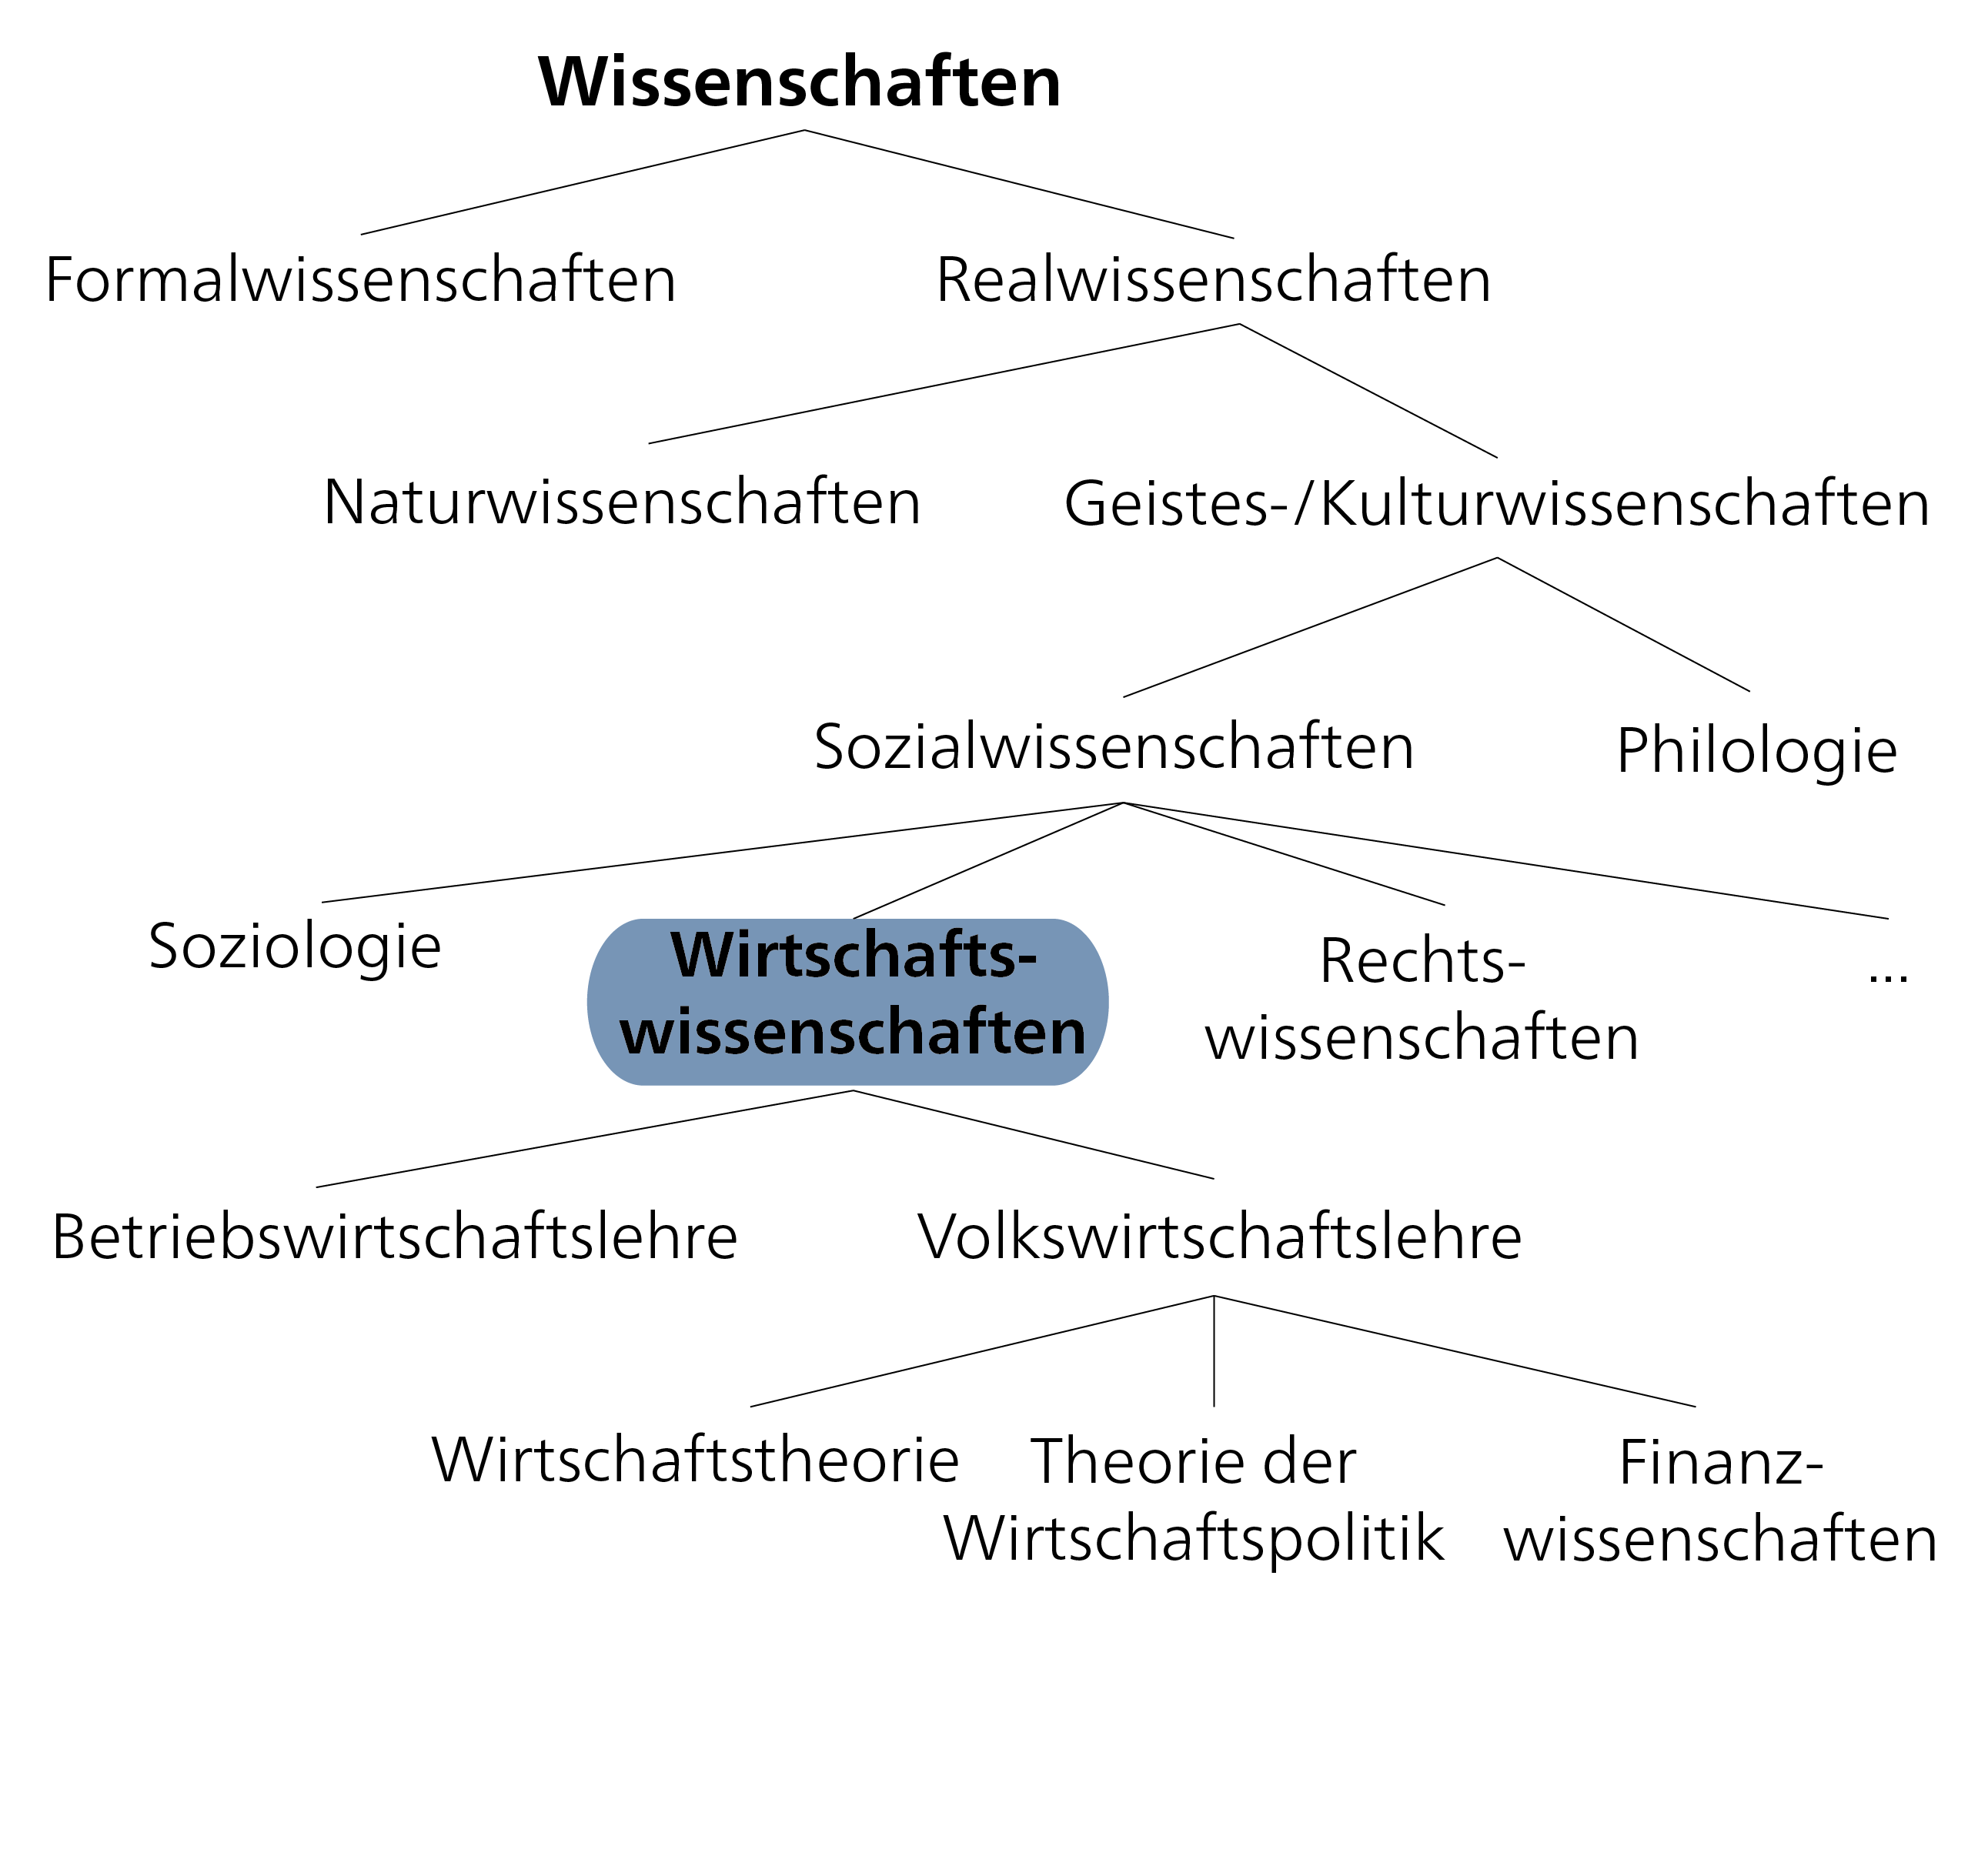
\includegraphics[keepaspectratio]{1_thinking-economics/images/fig1.png}}

}

\caption{Disciplinary location of the economic sciences. Source: Own
illustration after Engelkamp and Sell (2013, 3).}

\end{figure}%

\textbf{Business administration} ``is the study of the economic,
organisational, technical, and financial processes in companies and the
various economic institutions'' (Friedli et al. 2019, 16). Researchers
in this field develop a microeconomic perspective on the respective
object of study.

\textbf{Economics}, by contrast, does not examine what happens within
individual economic actors but the interplay between them -- that is, a
macroeconomic perspective. This course deals with this perspective.

Economics can be divided into \textbf{three larger subfields}:

\textbf{Economic theory}: describes economic theories and their
implications. It is divided into \textbf{microeconomics} (the behaviour
of individual households and firms and their coordination through
markets and prices). Microeconomics makes no statements about aggregate
economic relationships but examines the behaviour of individual firms
and households and their coordination process via the market by means of
price adjustments (Bontrup and Marquardt 2021, 1). In contrast,
\textbf{macroeconomics} deals with economy-wide phenomena and the
relationships between economic sectors and different markets. It
examines, for example, overarching economic indicators such as the
unemployment rate or inflation.

\textbf{Economic policy}: deals with state interventions in the economy
to increase societal welfare (Bontrup and Marquardt 2021, 2), for
instance through interventions such as cartel bans or the introduction
of minimum wages.

\textbf{Public finance} examines the various components of the state
budget, such as taxes or subsidies, and their mutual relationship. In
doing so, it implicitly examines questions about the role of the state
in resource allocation and in the distribution of income and wealth.

\end{tcolorbox}

\subsection[Understandings of economics in
history]{\texorpdfstring{Understandings of economics in
history\footnote{This short overview is based in part on Bäuerle et al.
  (2026).}}{Understandings of economics in history}}\label{understandings-of-economics-in-history1_intro-1}

The term economics first appears in the history of Western thought in
ancient Greece, as the study of household management. The word is
composed of two terms: \emph{oikos} (house) and \emph{nemein} (to manage
or arrange). In this understanding, economics dealt, among other things,
with questions of managing one's own property, planning and assessing
agricultural activities, selecting slaves, and the relationship between
husband and wife. Economics was strongly embedded in politics and ethics
and was meant to contribute to strengthening the \emph{polis}, the
city-state. The ultimate goal was the happy life, \emph{eudaimonia}. In
sharp contrast to economics stood so-called chrematistics, which aimed
at the accumulation of money instead of the happy life and was rejected
in ancient Greece.

In medieval Europe, the understanding of economics initially remained
closely tied to moral and religious ideas. Economic activity was not
understood as an independent area of society but was part of a divine
and moral order. The goal of economic activity was not the greatest
possible accumulation of wealth but securing a livelihood and the common
good. This understanding was strongly shaped by Scholasticism, in
particular by Thomas Aquinas (c.~1225-1274). At the centre were
questions about a just price (\emph{iustum pretium}), a just wage, and
the moral legitimacy of economic activities. Trade was accepted in
principle as long as it served the exchange of necessary goods. By
contrast, making profit purely for its own sake was considered
problematic. The charging of interest was judged particularly
critically, since money itself was regarded as unproductive and was not
supposed to serve the multiplication of money. The economy was thus
strongly embedded in ethical and societal norms.

This began to change only with the emergence of modern capitalism, the
expansion of trade, and industrialization, and an understanding of the
economy as an independent area of society gradually became established.
With the rise of mercantile capitalism and the Industrial Revolution,
classical political economy emerged in the 18th century. Representatives
such as Adam Smith (1723-1790), David Ricardo (1772-1823), or, later,
Karl Marx (1818-1883) were less interested in the management of
individual households than in the creation, distribution, and
development of the societal wealth of entire national economies. The
subject matter of economics thus shifted from household management to
the analysis of the production, distribution, and accumulation of
wealth. Questions such as these were at the centre: How does economic
prosperity arise? How is societal income distributed between labour,
capital, and land? The analyses focused on social classes -- for example
workers, owners of capital, and landowners -- and their relationships to
one another. The economy was understood as a societal process whose
development is shaped by institutions, property relations, and the
distribution of the societal surplus.

Towards the end of the 19th century, the so-called marginalist
revolution fundamentally changed the understanding of certain parts of
economics. The works of representatives of this new current, such as
William Stanley Jevons (1835-1882), Carl Menger (1840-1921), and Léon
Walras (1834-1910), formed the basis for the emergence of neoclassical
economics. At the centre of this new perspective was no longer the
production of societal wealth but the individual endowed with the
capacity for decision-making. The starting point of the analysis was now
households and firms that make rational decisions on markets under
conditions of scarce resources and maximize their utility or profit. The
economy was understood as the result of the decisions of many individual
economic subjects. This change meant a fundamental shift in perspective.
While classical political economy looked at the national economy, that
is, entire economies, and put social classes, production, and
distribution at the centre, neoclassical economics takes individual
markets above all as its frame of reference and focuses on individual
decisions and price mechanisms. With the works of John Maynard Keynes
(1883-1946), economy-wide relationships came into view again in the
mid-20th century, not only in Keynesian schools of thought but also in
neoclassical economics. Macroeconomics emerged on the basis of Keynes's
work.

History was by no means a linear development from one understanding of
economics to the next. Often, different understandings existed at the
same time, influencing, contradicting, and developing one another. The
perspectives outlined above are meant to make clear that the picture of
what the economy is has changed considerably over time and continues to
change. Moreover, present-day understandings build on these
developments, so it is also important to understand where certain
understandings come from and how they developed.

\subsection{Understandings of economics in the
present}\label{understandings-of-economics-in-the-present}

With the development of economic theories, different ideas have
developed about what economics actually studies. Two fundamentally
different ways of understanding economics can be distinguished. Karl
Polanyi already made this distinction in 1957 (Polanyi et al. 1957):

\begin{itemize}
\item
  On the one hand, economics can be understood through its
  \textbf{subject matter}: one determines \emph{which section of
  reality} one studies -- regardless of the analytical perspective.
  Medicine, for example, defines itself through its subject matter: the
  human body and its health. Polanyi calls this understanding the
  substantivist one. It places the economy as an empirical subject area
  at the centre of the investigation.
\item
  On the other hand, economics can be understood through a
  \textbf{specific analytical approach}. In this approach, the
  analytical approach is the starting point -- regardless of which area
  of reality it is used to study, that is, regardless of the subject
  matter. Polanyi calls this a formal understanding of economics. This
  analytical approach results from a logical derivation rather than from
  an empirical investigation.
\end{itemize}

In principle, almost all historical understandings defined themselves
through the study of their subject matter. In ancient Greece, for
example, this was the management of a household (how does one best
manage the land, supplies, and slaves of a household?). In the 17th and
18th centuries, it was the national economy (how does a country as a
whole become prosperous, for example through trade and gold?). In both
cases, it was clearly outlined \emph{what} was being talked about -- a
specific section of reality.

With the marginalist revolution, the current economic mainstream
increasingly departs from this principle, defines itself through its
analytical approach, and develops a formal understanding of economics.
Based on a definition by Lionel Robbins from the 1930s, economics is
described as a science that studies how people choose between
alternatives under conditions of scarcity in order to achieve their
goals. Robbins writes:

\begin{quote}
``Economics is the science which studies human behaviour as a
relationship between ends and scarce means which have alternative uses''
(Robbins 1932, 15).
\end{quote}

Put simply: economics studies how people use scarce means (time, money,
resources) to achieve their goals as well as possible -- no matter
\emph{what} the goals are, although it almost always involves maximizing
individual utility. A simple example: a student has only three hours in
the evening (a scarce resource) and must decide whether to study for the
exam, go jogging, or meet friends (alternative uses). Precisely such a
decision under scarcity is at the centre of the mainstream approach and
forms the analytical starting point of this understanding of economics.
Economics students are not infrequently introduced to ``the foundations
of economic thinking'' in a course. It is precisely about practising
this analytical approach as the basis of economics.

From this analytical starting point, the actions of actors in the
economy are then analysed, with a strong focus on markets, the price
mechanism, and utility-optimizing individuals. Markets form the
framework within which individuals try to optimize their utility through
decisions under scarcity. This means that questions outside this
framework often receive no attention. In this
\href{https://www.youtube.com/watch?v=D-6rQmHpGfE}{video}, the economist
Ha-Joon Chang talks about the neoclassical understanding, which, through
its underlying analytical starting point, already gives a certain
orientation and systematically screens out certain aspects (see also
Chang and Chang 2014). And because this approach is not tied to a
particular subject matter, in practice it is also applied to topics that
one would not intuitively call ``economic'' -- for example, the question
of why people marry or have children (analysed as an ``economic
decision'' under scarcity of, for example, time, money, and affection).
In 1992, the economist Gary Becker received the Nobel Memorial Prize in
Economic Sciences for precisely this extension of the field of
application.

Many other schools of thought, by contrast, continue to define economics
through its subject matter: the economy itself. They thus follow a
substantivist understanding. The subject matter, and above all its
boundaries (what belongs to the economy), can be defined in different
ways. For Polanyi, the substantivist understanding is about examining
how humans, as a society and in relation to their environment, provide
the means of subsistence and distribute material prosperity. Concretely,
this means questions such as ``How is bread produced and distributed?''
or ``Who gets how much of societal wealth?'' -- regardless of the
analytical approach used to examine these questions. As mentioned above,
however, there are also different views on how exactly this subject
matter should be delimited. \emph{Feminist economics}, for example,
emphasizes that activities outside the market, such as unpaid care work,
are a central area of the economy and must be included in the analysis.
\emph{Ecological economics} similarly emphasizes that the economy is
embedded in nature, that nature forms the basis of all economic
activity, and that it must therefore be included in economic analysis.
In line with the different understandings of the subject matter,
different schools of thought also focus on different aspects, such as
power structures, institutions, or economy-wide and societal
relationships and structures. In the section on pluralist economics (see
Chapter 1.5, \emph{Pluralist Economics}), we will look more closely at
what characterizes neoclassical economics (the mainstream) and get to
know some of the other schools of thought.

In this script, we follow a substantivist understanding and define
economics through the subject matter of the economy. In Chapter 2
(\emph{Scope of Economics}), we will then examine this subject matter in
more detail.

\begin{tcolorbox}[enhanced jigsaw, arc=.35mm, bottomrule=.15mm, bottomtitle=1mm, breakable, colback=white, colbacktitle=quarto-callout-caution-color!10!white, colframe=quarto-callout-caution-color-frame, coltitle=black, left=2mm, leftrule=.75mm, opacityback=0, opacitybacktitle=0.6, rightrule=.15mm, title={Further reading}, titlerule=0mm, toprule=.15mm, toptitle=1mm]

Ha-Joon Chang's book \emph{Economics: The User's Guide} offers an easy
introduction to topics in economics and gives a good overview of the
history and current debates. Depending on your interest, individual
chapters can also easily be consulted on their own.

Chang, Ha-Joon. 2014. \emph{Economics: The User's Guide}. First U.S.
edition. Bloomsbury Press.

\end{tcolorbox}

\section{History of Economic Thought}\label{history-of-economic-thought}

We have now looked briefly at different understandings of economics. In
this section, we want to engage a little more with the history of
economic theory and ask how economics itself has developed. The emphasis
is on the emergence of the dominant school of thought, neoclassical
economics.

\begin{selfstudyphase}
In the online version, you will find three video excerpts from Walter Ötsch's lecture on the history of economic theory (in German) at this point. Walter Ötsch describes how economics developed from a moral science under Adam Smith (1723-1790) into a science with a biologically determined image of the human under Thomas Malthus (1766-1834) and David Ricardo (1772-1823). In this process, metaphors from the natural sciences (clock system, balance equilibrium, computer information) come to bear more and more. The development of neoclassical economics was strongly shaped by this process.

Walter Ötsch is a professor at the University of Society Design (Hochschule für Gesellschaftsgestaltung) in Koblenz. As an economist and cultural historian, he researches and publishes on socio-political and economic topics such as populism and the societal role of markets.

You can find the full lecture at: https://www.youtube.com/watch?v=zS3QgFE5ASE
\end{selfstudyphase}

\begin{tcolorbox}[enhanced jigsaw, arc=.35mm, bottomrule=.15mm, bottomtitle=1mm, breakable, colback=white, colbacktitle=quarto-callout-tip-color!10!white, colframe=quarto-callout-tip-color-frame, coltitle=black, left=2mm, leftrule=.75mm, opacityback=0, opacitybacktitle=0.6, rightrule=.15mm, title={Excursus: History of homo oeconomicus}, titlerule=0mm, toprule=.15mm, toptitle=1mm]

The history of homo oeconomicus goes back at least to the mention of the
``economicus'' in Xenophon's work of the same name in the fourth century
BCE (Wilson and Dixon 2014, 11). In the long period until the founding
of modern economics by Adam Smith in the 18th century, various
conceptions of the economic man\footnotemark{} were used -- often
strongly shaped by the respective spirit of the age.

The concept of homo oeconomicus, as a rational utility maximizer, is
commonly located as early as Smith, since he recognizes self-love as a
central human characteristic in behaviour. But as so often when it comes
to Smith's concepts, this common portrayal is idealized. Besides
self-love, Adam Smith identifies further human characteristics that are
central to behaviour. Smith paints a much more complex picture of human
behaviour than the reduced version of the modern homo oeconomicus does
(Hill 2012). Smith's dense description of the economic man makes it
impossible to model him or to work with him mathematically (Morgan 2006,
2012). This was to change over time through a deliberate reduction of
the description of the economic man.

Thomas Robert Malthus and David Ricardo already used somewhat more
reduced versions of the \emph{economic man} at the beginning of the 19th
century, which already show a certain model character (Morgan 1996,
2006, 2012). John Stuart Mill (1806-1873) took this further and reduced
the economic man to the characteristics considered central to the
economic domain: the desire to accumulate wealth, the aversion to work,
and the desire for luxury goods (Robson and Mill 1996). Although the
model of the economic man was reduced in Malthus, Ricardo, and Mill, it
could not yet be used, and was not used, in the way it is today.

A decisive foundation for this development was laid by William Stanley
Jevons (1835-1882) and Francis Edgeworth (1845-1926) towards the end of
the 19th century. Alongside Alfred Marshall (1842-1924), Léon Walras
(1834-1910), and Vilfredo Pareto (1848-1923), they are regarded as
important founders of neoclassical economics and were part of the
marginalist revolution. Like some other economists with a background in
mathematics or physics, the two economists were willing to make
economics a natural science. The neoclassical economists were convinced
that the analytical and deductive method should also be the royal road
for economics. Jevons justified the necessity of mathematics for
economics simply by the fact that economics deals with quantities
(Jevons 1879, 4). This group of economists took their orientation from
physics and physical concepts. Irving Fisher (1867-1947), another of the
first neoclassical economists, explicitly used various mechanical or
hydraulic concepts for his theories and applied them to the economy.

\begin{figure}[H]

{\centering \pandocbounded{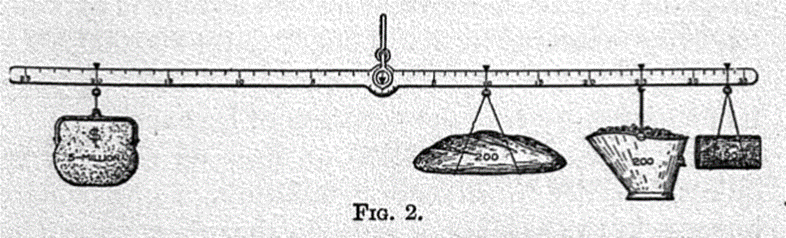
\includegraphics[keepaspectratio]{1_thinking-economics/images/fig2.png}}

}

\caption{Fisher's mechanical balance of exchange, used to represent the
quantity theory of money (Fisher 1922, 21).}

\end{figure}%

\begin{figure}[H]

{\centering \pandocbounded{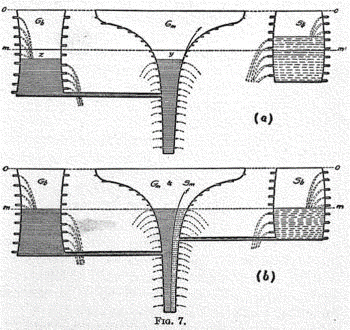
\includegraphics[keepaspectratio]{1_thinking-economics/images/fig3.png}}

}

\caption{Fisher uses a hydraulic model to represent purchasing power in
a bimetallism system (Fisher 1922, 119).}

\end{figure}%

The idea of equilibrium itself is a concept borrowed from physics. This
fixation on physics is also described as \emph{physics envy}, and
Mirowski shows that this orientation towards physics was a fundamental
driver in the development of the history of theory (Mirowski 1989, 396).
The explicit analogy to physics in economics persists well into the 20th
century. A good illustrative example of this, and of economists' basic
toolbox, is the
\href{https://www.youtube.com/watch?v=rAZavOcEnLg}{machine} built by
William Phillips (1914-1975) in the 1940s to represent the British
economy. The development of homo oeconomicus is accordingly also
exemplary of the mechanistic worldview that emerged in neoclassical
economics, as Walter Ötsch describes it in his lecture.

Among other things, the complexity of the \emph{economic man} stood in
the way of applying mathematics to economics. Jevons therefore attempted
to reduce this complexity. Shaped by the utilitarianism of Jeremy
Bentham (1748-1832), Jevons reduced the seven criteria Bentham had
formulated, which are central to calculating utility and thus influence
human action, to just two, on the grounds that only these were
economically relevant (Jevons 1879, 17). In this way, Jevons was able to
work mathematically with the economic man (Reiss 2000). This abstraction
and objectification of economics and of the economic man is most vividly
illustrated by the conceptions of Francis Edgeworth and, later, Frank
Knight. Edgeworth speaks of the economic man as a ``pleasure machine''
and Knight of the ``slot machine'' (Morgan 2006). Pareto's use of his
``homo oeconomicus'' also grounds an analysis of the human from a
mechanical viewpoint. Pareto writes: ``Just as analytical mechanics
treats material points and rigid bodies, mathematical economics
considers an abstract human being, a homo oeconomicus'' (Pareto and
Meyer 1902, 1100).

With the marginalist revolution, homo oeconomicus became the focus of
economics, which stands in strong contrast to the classical economists
(such as Smith, Malthus, Ricardo, and Marx), who focused predominantly
on class analysis. Moreover, the abstraction now enabled modelling and
mathematical applications, which was meant to bring economics closer to
the natural sciences. The rational, utility-maximizing agent became the
foundation of economics. The rational choice theory behind it was
subsequently developed further and adapted (for example through the
concept of bounded rationality) but remains in its fundamentals to this
day.

The history behind this development shows that it was not a natural one
but that a particular orientation of economics was deliberately pushed
forward. The neoclassical orientation, for example, makes it impossible
to recognize and analyse structural problems, since the focus is on
marginal changes in certain indicators (for example inflation or
interest rates). The work of the 2019 winners of the Nobel Memorial
Prize in Economic Sciences, Abhijit Banerjee, Esther Duflo, and Michael
Kremer, seems exemplary of this. In their research on poverty reduction,
they use experiments (so-called \emph{randomized controlled trials}) to
examine the effects of specific individual measures to reduce poverty.
The analysis (and thus also a change) of the structural causes of these
people's poverty falls out of view here.

This development of economics, as outlined here, was strongly criticized
right from its emergence. Criticism of the orientation, the fixation on
analytical models, and the strong abstractions from the real world
continues to this day. In view of the weaknesses of neoclassical
economics that have increasingly been exposed in the years since the
2008 financial crisis, Alfred Marshall's concerns about this development
have become topical again. In 1881, in a commentary on Edgeworth's
``Mathematical Psychics'', Marshall wondered whether Edgeworth would
succeed in preventing mathematics from running away with him and driving
him out of sight of the actual facts of the economy (Vazquez 1995, 251).

\end{tcolorbox}

\footnotetext{In this text, the English term economic man is used when
the concern is, in general, the idea of an economic agent. This is
because the term homo oeconomicus stands for the currently dominant
conception, and economic man is used in this sense in the (predominantly
English-language) literature. The term is problematic in that it implies
the exclusion of an economic woman. If we look at the orientation of
economics today and in history, however, such a portrayal of economics
is unfortunately not that far-fetched, as feminist economics shows us.}

\begin{tcolorbox}[enhanced jigsaw, arc=.35mm, bottomrule=.15mm, bottomtitle=1mm, breakable, colback=white, colbacktitle=quarto-callout-caution-color!10!white, colframe=quarto-callout-caution-color-frame, coltitle=black, left=2mm, leftrule=.75mm, opacityback=0, opacitybacktitle=0.6, rightrule=.15mm, title={Further reading}, titlerule=0mm, toprule=.15mm, toptitle=1mm]

If you are interested, you can also watch the
\href{https://www.youtube.com/watch?v=zS3QgFE5ASE}{entire lecture by
Walter Ötsch} (in German).

Lisa Herzog (2014) in her book \emph{Der Wert des Marktes} {[}The Value
of the Market{]}: \href{https://ilias.unibe.ch/go/file/3803489}{The
defence of the market from the 18th century to the present (pp.~13-27)}
(in German).

\href{https://www.youtube.com/watch?v=kgAKCvhDHIw}{Lecture by Lisa
Herzog} on the history of ideas as an interdisciplinary approach to
economics (in German).

Hans Christoph Binswanger (2006) in his book \emph{Die Wachstumsspirale}
{[}The Growth Spiral{]}:
\href{https://ilias.unibe.ch/go/file/3803487}{From Aristotle to Walras
and back -- Aristotle as a precursor of modern economics (pp.~377-387)}
(in German).

The following further reading is for students who want to dive somewhat
deeper and engage more intensively with the history of theory:

\begin{itemize}
\tightlist
\item
  Ambler, Lucy, Joe Earle, and Nicola Scott. 2022. ``Whitewashes
  History''. In \emph{Reclaiming Economics for Future Generations},
  Manchester Capitalism Ser, Manchester: Manchester University Press,
  118--60.
\item
  McCloskey, Deirdre N. 1998. \emph{The Rhetoric of Economics}. 2nd
  ed.~Rhetoric of the Human Sciences. Madison, Wis: University of
  Wisconsin Press.
\item
  Mirowski, Philip. 1989. \emph{More Heat than Light: Economics as
  Social Physics, Physics as Nature's Economics}. Cambridge: Cambridge
  University Press. https://doi.org/10.1017/CBO9780511559990.
\end{itemize}

\end{tcolorbox}

\section{How Do These Different Understandings of Economics Come
About?}\label{how-do-these-different-understandings-of-economics-come-about}

Philosophy of science distinguishes between two basic questions:
\textbf{Ontology} asks what reality actually is. \textbf{Epistemology}
asks how we can gain knowledge about this reality. These questions seem
abstract but have important consequences for our understanding of the
economy.

Many economists, especially in neoclassical economics and the economic
mainstream, hold, for example, that economic theory must be independent
of images of the human and of society, and thus also independent of
social philosophies and values. According to this view, economic theory
should be neutral and free of values and able to formulate universally
valid laws. This view understands economics as a ``positive'' science.
\textbf{Positivism} results from an ontological and an epistemological
position, even if these are not always made explicit. Ontologically,
positivism assumes that there is a social and physical nature or reality
that exists independently of the historical context and is subject to
universal laws. These laws exist independently of our perception.
Epistemologically, positivism also assumes that laws can be objectively
recognized and described. Scientific methods serve this purpose and can
bring this reality to light. Since positivism is mainly associated with
the natural sciences (although this view is not shared by everyone there
either), a positivist conception of economics often draws strongly on
the natural sciences. It claims to describe the world ``as it is''
without having previously made a value judgement or taken a particular
perspective. Accordingly, this view distinguishes between positive
statements (how the world is) and normative statements (how the world
should be) and argues that these spheres can be clearly separated.
Economics should focus on positive statements. For economics, this
position consequently means that there cannot necessarily be different
schools of thought that reach different conclusions, since there is one
objective reality that we can also describe as such.

Critics argue that such a clear separation between positive and
normative statements, between facts and values, is not possible for
social sciences such as economics and accordingly makes an objective and
value-free analysis impossible (see, for example, DeMartino et al.
2016). Hilary Putnam argues that facts and values are often not clearly
separable but intertwined (Putnam 2002). Here, too, we find ontological
and epistemological basic assumptions that lead to such conclusions. The
term \textbf{``constructivism''} can serve as a collective term for many
epistemological currents. All of these currents assume, in one way or
another, a socially constructed reality. Although some currents assume
an objective reality ontologically, they agree that the way we generate
knowledge and what we recognize as knowledge is historically and
socially specific. Accordingly, constructivism supports the position
that scientific insights are always also shaped by social contexts,
historical developments, and normative presuppositions. Economic
concepts and theories are therefore always already shaped in their
construction by values and worldviews. Which questions are asked and
which answers seem plausible thus also depends on the respective
perspectives of the researchers. For economics, this means that
different theoretical approaches can legitimately arrive at different
interpretations of economic reality or realities.

Our position: We consider a strict separation of the positive and the
normative impossible and orient ourselves towards a constructivist
understanding of science. The different views on how economics can be
defined already show that value judgements are always made implicitly.
One perspective can focus on the efficient allocation of scarce
resources in a society, another on overcoming poverty and meeting the
basic needs of all people in an economy. As soon as we adopt one
perspective at the expense of another, we have made a first value
judgement.

This does not mean, however, that there are no facts or that all
approaches are equally valid, nor that there is no reality independent
of our interpretation -- we can only approach it more or less closely.
Like any other science, economics has to orient itself towards
scientific principles and methods. In addition, assumptions and value
judgements should be made explicit and transparent.

The dispute over whether economics is free of any value judgements or
not has run from the emergence of economics as its own field of science
to the present and has not been conclusively resolved. Two quotes from
two well-known economists of the first half of the 20th century
illustrate this:

\begin{quote}
``Economics deals with ascertainable facts; ethics with valuations and
obligations. The two fields of enquiry are not the same plane of
discourse'' Lionel Robbins in An Essay on the Nature and Significance of
Economic Science (Robbins 1932, 132).
\end{quote}

\begin{quote}
``As against Robbins, Economics is essentially a moral science. That is
to say, it employs introspection and judgement of value'' John M. Keynes
in a letter to Sir Roy Harrod, 4 July 1938, in (Atkinson 2009, 791)
\end{quote}

\begin{tcolorbox}[enhanced jigsaw, arc=.35mm, bottomrule=.15mm, bottomtitle=1mm, breakable, colback=white, colbacktitle=quarto-callout-tip-color!10!white, colframe=quarto-callout-tip-color-frame, coltitle=black, left=2mm, leftrule=.75mm, opacityback=0, opacitybacktitle=0.6, rightrule=.15mm, title={Excursus: Do assumptions have to be realistic?}, titlerule=0mm, toprule=.15mm, toptitle=1mm]

Besides the criticism of the value judgements implied in neoclassical
economics, its explicit framework of assumptions also leads to
controversial discussions, in particular over the extent to which
assumptions must represent reality realistically. Do the initial
assumptions, such as the existence of perfect competition, have to be
realistic in order to gain valuable insights? At first glance, the
finding seems clear: unrealistic or incomplete assumptions would also
have to lead to false conclusions. According to the American Paul
Samuelson (1915-2009), one of the best-known economists of the 20th
century, it is impossible to infer true insights from demonstrably false
assumptions. Proponents of so-called \textbf{instrumentalism}, however,
argue differently. In view of the complexity of human behaviour, they
say, one must positively abstract in the analysis and leave out what is
inessential. The American economist Milton Friedman (1912-2006), also
one of the best-known economists of the 20th century, in search of an
efficient method for discovering far-reaching insights and policy
recommendations, even establishes an extreme anti-realist position.
Analysing within a make-believe world is declared an unproblematic
necessity:

\emph{``Truly important and significant hypothesis will be found to have
assumptions that are widely inaccurate descriptive representations of
reality, and in general the more significant the theory, the more
unrealistic the assumption. {[}\ldots{]} To be important, therefore, a
hypothesis must be descriptively false in its assumptions''} Milton
Friedman (1953) {[}p.~14{]}.

\end{tcolorbox}

\section{Styles of Thought and Thought
Collectives}\label{styles-of-thought-and-thought-collectives}

As discussed in the previous section, economic theories are always
shaped by value judgements and worldviews. There is therefore no clearly
objective economic theory but a multitude of perspectives that make it
possible to analyse and describe economic phenomena. There is no neutral
``view from nowhere'' or purely objective perspective, since our
perception is shaped by numerous influences, such as our education, our
social and cultural environment, our language, our material living
conditions, and our personal experiences. These influences shape our
perspective on looking at the world.

Perspectives can also be regarded as ``glasses'': some glasses allow a
view of the big picture, while others serve to identify details and
subtleties. These different glasses mean that we can see the world in
different colours and shades. Nevertheless, this does not mean that the
world can be interpreted arbitrarily. There are limits to
multiperspectivity, which require economics to orient itself towards
scientific principles and methods.

In the philosophy of science, perspectives are also referred to as
\textbf{paradigms or styles of thought}. Ludwik Fleck (1896-1961), a
Polish physician and philosopher of science, developed the concept of
the style of thought decades before Thomas Kuhn (1922-1996), who created
the better-known concept of the paradigm. In 1944, Fleck was deported to
the Buchenwald concentration camp, where he was made to develop a typhus
vaccine. However, he supplied the SS only with a placebo and distributed
the real medicine to fellow prisoners.

In his scientific work, Fleck emphasized the \textbf{dependence of
thinking on values and contexts}. He objected to the idea that knowledge
is objective, neutral, and universal. He argued that the production and
use of knowledge take place in specific environments, which influences
their meaning and effect. Knowledge is used differently in concentration
camps than in NGOs or corporate research departments. Knowledge is
always embedded in institutions and power structures, and scientists are
influenced by their environment and experiences.

\textbf{Thought collectives} are groups of people who share a common
style of thought and use particular concepts and methods. Thought
collectives thus use a particular pair of glasses to look at the world.
These thought collectives often resist change and resist further
developments of their way of thinking. Since, as Fleck emphasized,
people can think, argue, and understand in fundamentally different ways,
people who belong to different thought collectives often have difficulty
following the trains of thought of other styles of thought.

Fleck's insights show that science and thinking are by no means
independent of social, cultural, and historical contexts. They make
clear the \textbf{diversity of perspectives} from which scientific
problems can be viewed and underline that no single theory or way of
thinking can capture the whole of reality completely. Instead, different
styles of thought and thought collectives are able to provide diverse
insights and enrich the understanding of complex phenomena. This leads
to different economic policy recommendations and offers a broad range of
approaches to solving complex challenges.

\subsection{Thought collectives in
economics}\label{thought-collectives-in-economics}

As already indicated several times, economics too consists of a
multitude of different thought collectives that take particular
perspectives, or styles of thought, based on value judgements and
worldviews. This diversity of styles of thought is described by the term
``pluralist economics''. At present, economics is strongly dominated by
one style of thought, neoclassical economics, which is often described
as the economic mainstream. Nevertheless, or perhaps precisely for this
reason, it is central that students have a rough overview of the
different styles of thought in order to gain a comprehensive
understanding of the economy. Accordingly, the next section briefly
introduces pluralist economics, in which students can then explore the
different styles of thought according to their interests. We believe,
however, that students should not only get to know the style of thought
of the dominant thought collective but also gain insight into how the
styles of thought in economics have developed and which other styles of
thought exist in economics. In the next section, you will get an
overview of the different styles of thought in economics. In what
follows, we will mostly call them schools of thought rather than styles
of thought, since this is what they are usually called.

\begin{tcolorbox}[enhanced jigsaw, arc=.35mm, bottomrule=.15mm, bottomtitle=1mm, breakable, colback=white, colbacktitle=quarto-callout-caution-color!10!white, colframe=quarto-callout-caution-color-frame, coltitle=black, left=2mm, leftrule=.75mm, opacityback=0, opacitybacktitle=0.6, rightrule=.15mm, title={Further reading}, titlerule=0mm, toprule=.15mm, toptitle=1mm]

\href{https://ilias.unibe.ch/go/file/3803488}{Yuval Harari and the
Peugeot legend in his book \emph{Sapiens: A Brief History of Humankind}}
(in German)\\
His thesis: the truly sufficient difference between us and the other
animals is the ability to create cooperative networks in which sometimes
millions of complete strangers work together towards shared goals. We
can cooperate with one another on a large scale because we follow shared
intersubjective fictions. We work successfully with strangers because,
like them, we believe in things such as gods, nations, money, or human
rights. And yet none of these things exists outside the stories that
people invent and tell one another. There are no gods in the universe,
no nations, no money, and no human rights -- except in the shared
imagination of human beings.

\href{https://pitchforkeconomics.com/episode/what-is-the-trick-in-trickle-down/}{Podcast
with Yuval Harari on ``trickle-down economics'': What is the trick in
trickle down?}\\
How do wealthy elites and their neoliberal mouthpieces manage to
convince us that what benefits them -- tax cuts, deregulation, and the
like -- also benefits all of us? And why, of all things, are the minimum
wage, paid overtime, or sick days considered a danger to the economy?
Economics is ultimately a story we tell ourselves to explain who gets
what -- and why. The podcast explores the question: What might a better
story look like?

\end{tcolorbox}

\section{Pluralist Economics}\label{pluralist-economics}

As has been indicated several times, there are different schools of
thought based on different understandings and perspectives. Some of the
differences arise from fundamental philosophical questions, from
methodological approaches, or from differences in content (for example
different foci). Despite its diversity, present-day economics is
dominated by the neoclassical school of thought. The dominance was
particularly strong towards the end of the 20th century and in the
2000s. The great financial crisis of 2008 boosted the rise of theories
that had been marginalized until then, since neoclassical economics was
evidently inadequate to fully explain this crisis. Nevertheless,
neoclassical economics remains dominant in the economic sciences to this
day.

To be able to meet the complexity of present-day challenges, we consider
it essential to be able to draw on this diversity of theories and tools.
The dominance of a single school of thought carries the risk that we
perceive certain phenomena from only one perspective and can accordingly
offer only solutions that follow from that perspective, as the following
quote illustrates:

\begin{quote}
``I suppose it is tempting, if the only tool you have is a hammer, to
treat everything as if it were a nail'' Abraham Maslow in Psychology of
Science (Maslow 1966, 15).
\end{quote}

This short section is therefore meant to give you the opportunity to
engage with the diversity of the economic sciences, that is, pluralist
economics. Engaging with different schools of thought should enable
students to perceive and reflect on economic questions in a more
differentiated way. It will not be possible, however, to cover all
schools of thought in depth. In the self-study phase, you will find
opportunities to familiarize yourself independently with the different
schools of thought if you are interested. We are also happy to provide
further material if you would like to engage more intensively with
pluralist economics or individual schools of thought. In addition, for
students who want to engage more intensively with different schools of
thought, we offer the course ``Introduction to pluralist economics'' in
the spring semester.

Before you set out to explore in the ``scavenger hunt through pluralist
economics'', this
\href{https://www.youtube.com/watch?v=NdbbcO35arw}{video} by Professor
Ha-Joon Chang of SOAS University gives you a rough overview of different
schools of economic thought and how they can (or could) lead to
different economic policy programmes.

\subsection{Scavenger hunt through pluralist
economics}\label{scavenger-hunt-through-pluralist-economics}

Exploring Economics is an open project of the Network for Pluralist
Economics, which cooperates with various international actors in
designing the e-learning platform. The network consists of many local
groups and individuals. There are numerous ways to take part and
contribute. We believe that this open platform offers a great many good
contributions. We have therefore designed a scavenger hunt through the
platform so that you can get to know it in a playful way.

\begin{tcolorbox}[enhanced jigsaw, arc=.35mm, bottomrule=.15mm, bottomtitle=1mm, breakable, colback=white, colbacktitle=quarto-callout-note-color!10!white, colframe=quarto-callout-note-color-frame, coltitle=black, left=2mm, leftrule=.75mm, opacityback=0, opacitybacktitle=0.6, rightrule=.15mm, title={Exercise -- Pluralist economics}, titlerule=0mm, toprule=.15mm, toptitle=1mm]

In this learning section, you solve the crossword puzzle
\href{https://ilias.unibe.ch/go/file/3803483}{``Tour through economic
theories''} (in German) using the
\href{https://www.exploring-economics.org/en/}{Exploring Economics
platform}. Under the heading ``Orientation'' there, you will find
solutions to the terms sought in the puzzle. This gives you an overview
of the different schools of thought in economics and of how these
perspectives influence research and its results. This exercise is
voluntary and is meant to allow you to get to know pluralist economics
in a playful way. The crossword puzzle will not be discussed in the
in-person session. You are welcome, however, to use the office hours to
discuss questions and points of uncertainty.

\end{tcolorbox}

\begin{figure}[H]

{\centering \pandocbounded{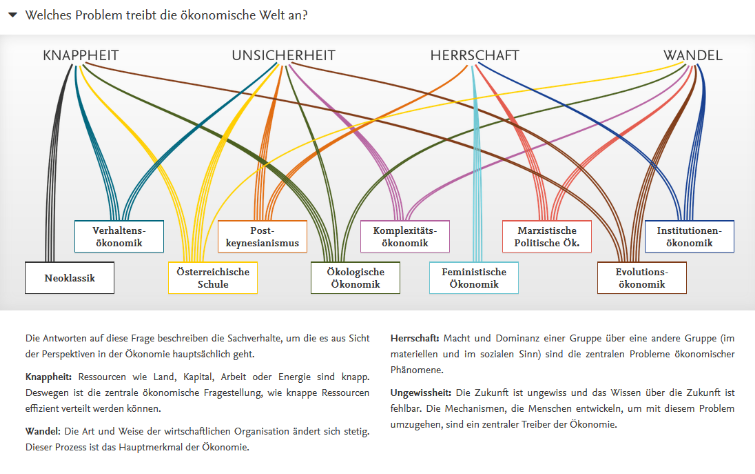
\includegraphics[keepaspectratio]{1_thinking-economics/images/fig4.png}}

}

\caption{Excerpt from the Exploring Economics website, categorizing the
different schools of thought according to the question. Source:
\href{https://www.exploring-economics.org/en/}{Exploring Economics}.}

\end{figure}%

In this course, we explicitly orient ourselves in what follows towards
an understanding that defines economics through its subject matter and
takes no theoretical orientation as the basis of our understanding of
economics. Accordingly, this understanding also leaves room to draw on
many different approaches and schools of thought to understand economic
relationships. In what follows, we therefore first want to approach the
subject matter and get to know some basic terms and concepts.

\section{Sustainable Economics: The Approach of This
Script}\label{sustainable-economics-the-approach-of-this-script}

\emph{↗ Textbook chapter 5}

As we have seen in this chapter, there is no single economics but a
multitude of schools of thought with different basic assumptions,
questions, and perspectives on economic phenomena. We have also
established that scientific perspectives are never entirely neutral but
always already contain value judgements. This script follows the
approach of \textbf{sustainable economics}. The guiding question is how
our economy can be designed sustainably. Sustainable economics thus
explicitly has a normative character. We will see that answering this
question also depends strongly on the specific understanding of
sustainability, but also on fundamental questions about the goals of
economic activity and on the understanding of the subject matter of
economics itself.

A first point of approach is the contrast often drawn in debates about a
more sustainable economy, that between \textbf{green growth} and
\textbf{post-growth}\footnote{The term degrowth is also often used.
  Although the two terms are not entirely identical, they largely
  overlap. For simplicity, we will therefore use the term post-growth
  throughout. In our view, the strength of the term post-growth lies
  above all in the fact that it does not emphasize a possible shrinkage
  of the economy so much as the necessary growth independence.}.

Green growth approaches (e.g. OECD 2011; World Bank 2012) assume that
economic growth and declining environmental pressure can be reconciled
-- the economy is meant to grow but become ``green''. Post-growth
approaches (e.g. D'Alisa et al. 2016; Jackson 2009; Seidl and Zahrnt
2010), by contrast, argue that growth itself -- and the growth
imperative of capitalist economies associated with it (see Chapter
2.1.3, \emph{Economic growth} and Chapter 2.5.4, \emph{What actually
makes an economic system capitalist?}) -- is a central cause of
ecological problems.

This polarization is didactically helpful because it makes a real debate
visible. But it is also misleading if taken too literally: in practice,
it is rarely an either-or between two closed camps but a question of how
to design an economy that respects ecological limits while enabling a
good life for all.

\begin{figure}[H]

{\centering \pandocbounded{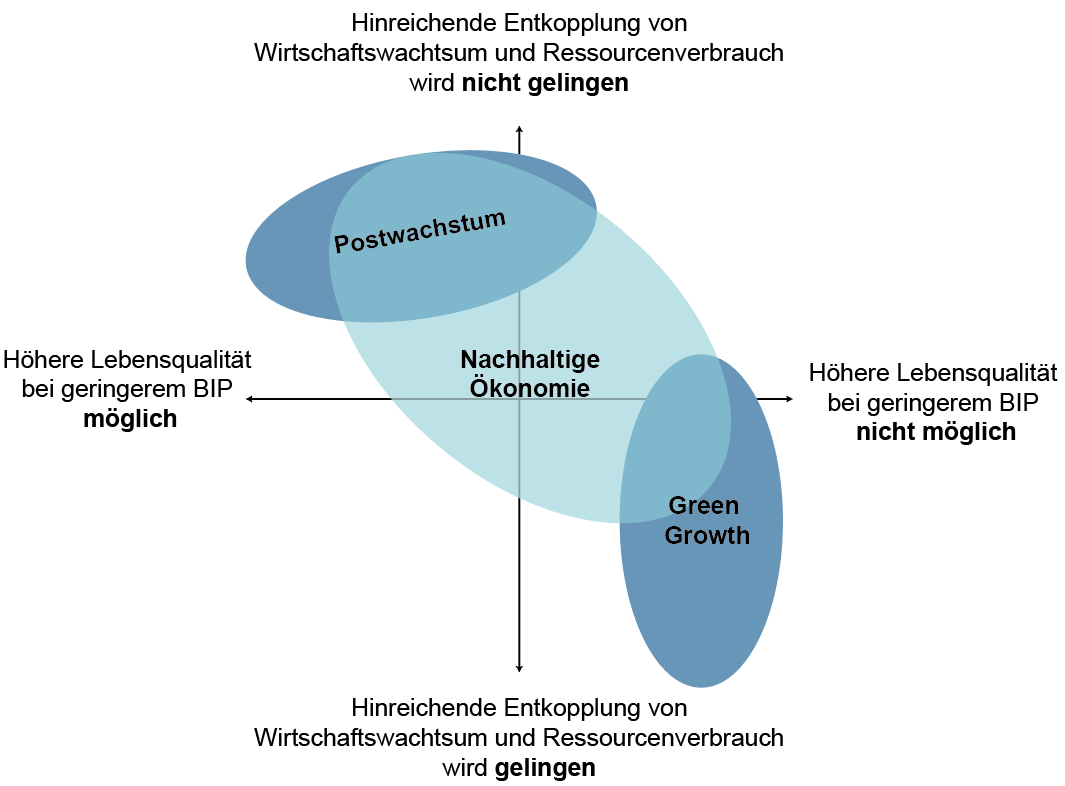
\includegraphics[keepaspectratio]{1_thinking-economics/images/fig5.png}}

}

\caption{Figure 5. Sustainable economics. Source: Own illustration,
adapted from Petschow et al. (2018, 22).}

\end{figure}%

This is precisely where sustainable economics comes in: it does not
position itself at either of the two poles but asks what ecological and
social sustainability require, and only then derives what role growth
can or must play. It thus does not start with a fixed answer (``more
green growth'' or ``shrinkage'') but asks instead about the goals of
economic activity.

We will not yet present a definition of sustainable economics here but
will approach an understanding of it over the next chapters. In the next
chapter, we approach the subject matter of economics and address, among
other things, the question of what the goal of economic activity
actually is and what we understand by prosperity. After that, we look at
the ecological and social limits and challenges of our current economic
system. Sustainable economics aims to develop approaches to overcoming
these challenges. Then, in Chapters 4 and 5, we look at possible
strategies and roles of the state. In the concluding chapter of this
script, we then want to draw a clearer picture of sustainable economics
from all this.

\chapter{Scope of Economics}\label{scope-of-economics}

As we discussed in the previous chapter, economics can be defined in two
ways: through an analytical approach (as the mainstream does) or through
a subject matter -- that is, through \emph{what} economics deals with in
terms of content. In this chapter, we approach the subject matter and
ask concretely: What is actually the object that economics studies?

You will find that even basic questions -- such as ``What is work?'' --
are answered differently. The reason is that, depending on one's
understanding of the economy, one also understands its individual
aspects differently. As introduced above, we therefore distinguish
different schools of thought in economics. Each of these schools of
thought brings its own understanding of the economy and accordingly
looks at economic questions differently.

To approach the scope of economics, we follow a simple means-end logic:
we begin with the \emph{goal} of economic activity -- prosperity -- and
then ask \emph{with what} (resources, production) and \emph{how} (market
or economic system) this goal is achieved. This chapter is accordingly
structured as follows:

\begin{itemize}
\item
  \textbf{Prosperity in a changing world:} What is the goal of economic
  activity -- what do we understand by prosperity?
\item
  \textbf{Forms of provision in the economy:} What is needed for this
  prosperity to arise in the first place?

  \begin{itemize}
  \item
    (Re)production factors: What is needed for goods and services to
    come into being?
  \item
    Land -- Can we replace nature with technology at will?
  \item
    Capital -- Why do some people own capital and others do not -- and
    how does it differ from money?
  \item
    Labour -- Why do I earn as much as I do -- and why is some work,
    such as care work, often not paid at all?
  \item
    Types of goods: Is the sun a public good -- and which properties
    determine how a good is treated economically?
  \item
    External effects: Why does a flight often cost less than a train
    ride -- even though it harms the environment much more?
  \end{itemize}
\item
  \textbf{Abstract markets or capitalist production system:} How is it
  coordinated who uses these resources and how, and who receives the
  result?

  \begin{itemize}
  \item
    The neoclassical perspective: Does anyone need to steer the economy
    at all -- or does it regulate itself?
  \item
    The political-economy perspective: Who actually determines the rules
    of the market -- and in whose interest?
  \item
    What is capitalism? -- What actually makes an economic system
    capitalist?
  \item
    Why do companies (and entire economies) actually have to grow
    constantly?
  \item
    Are financial crises accidents -- or built into the system?
  \end{itemize}
\end{itemize}

\begin{tcolorbox}[enhanced jigsaw, arc=.35mm, bottomrule=.15mm, bottomtitle=1mm, breakable, colback=white, colbacktitle=quarto-callout-note-color!10!white, colframe=quarto-callout-note-color-frame, coltitle=black, left=2mm, leftrule=.75mm, opacityback=0, opacitybacktitle=0.6, rightrule=.15mm, title={Overarching guiding question of this chapter}, titlerule=0mm, toprule=.15mm, toptitle=1mm]

How does a society ensure at all that the needs of its members are met?

\end{tcolorbox}

We are aware that, for students without a background in economics, there
are many new terms. The aim of this chapter is therefore not that you
know all topic areas in detail afterwards but rather that you gain a
solid overview of the scope of economics. For students of economics, the
chapter serves at the same time as a review and as a broader
contextualization of existing knowledge.

\begin{selfstudyphase}
Several in-depth questions are listed for each subsection. On the one hand, these serve to check your own knowledge of the respective area; on the other hand, they are also meant to prompt thought and reflection. If questions remain open on individual contents, or if you need a more in-depth engagement, you can use the forum for questions and discussions on the content. Here, students can support one another during the self-study phase, and the lecturers have the opportunity to answer questions for all course participants together. You are also welcome to use the office hours on 1 October 2026 for questions and a deeper engagement. Please register for them via ILIAS by 30 September at 23:55. Of course, questions and thoughts can also be discussed in the in-person sessions.
\end{selfstudyphase}

\section{Prosperity in a Changing
World}\label{prosperity-in-a-changing-world}

\emph{↗ Textbook chapter 3}

\begin{tcolorbox}[enhanced jigsaw, arc=.35mm, bottomrule=.15mm, bottomtitle=1mm, breakable, colback=white, colbacktitle=quarto-callout-note-color!10!white, colframe=quarto-callout-note-color-frame, coltitle=black, left=2mm, leftrule=.75mm, opacityback=0, opacitybacktitle=0.6, rightrule=.15mm, title={Guiding question}, titlerule=0mm, toprule=.15mm, toptitle=1mm]

What is the goal of economic activity -- what do we understand by
prosperity?

\end{tcolorbox}

When we ask about the scope of economics, we inevitably encounter the
question of its goal: What is the purpose of economic activity in the
first place? An obvious but incomplete answer is: to create prosperity.
But what exactly is meant by ``prosperity''?

At least in Western societies, prosperity is often understood
materially, that is, as how much money we have and what things we can
afford with it. But prosperity could just as well include life
expectancy, education, social relationships, leisure time, an intact
environment, or subjective well-being. Depending on how prosperity is
defined, what counts as ``good'' economic development also changes. This
question is thus anything but neutral: it implicitly determines what a
society should strive for in the first place.

Because prosperity is so multifaceted, its measurement is
correspondingly difficult and contested. The most widespread index for
measuring prosperity to this day is gross domestic product (GDP). It is
omnipresent in everyday life, in politics, and in the media and is
regarded in many places as the most important economic indicator of all.
In what follows, we therefore first look at what GDP actually measures
-- and what it does not.

\subsection{Gross domestic product (GDP) as an indicator of (material)
prosperity}\label{gross-domestic-product-gdp-as-an-indicator-of-material-prosperity}

GDP is regarded as the main indicator of a nation's prosperity. It
measures the total value of all goods and services produced in a country
within a year, after deduction of all intermediate inputs. The concept
of GDP in its current form was developed only in the 1930s -- first
attempts to measure a country's prosperity go back to the work of
William Petty in the 17th century -- to combat the Great Depression and
to plan armaments spending in the Second World War in the USA and
England (Schmelzer and Vetter 2019, 57--59). A precondition for this was
also the invention of the ``economy'' as a separate sphere of social
life that can be statistically recorded and measured (Schmelzer and
Vetter 2019, 57). Despite its present widespread use, GDP is also
constantly criticized. Even economists who advanced the development of
GDP warned against using GDP as a general measure of prosperity. Simon
Kuznets (1901-1985), one of the most prominent economists in this field,
said: \emph{``However one may use them, such figures {[}\ldots{]} seem
very useful; they seem to measure and make comparable something clearly
defined and significant. But on closer inspection, it turns out that the
impression that such estimates are clear and unambiguous is
deceptive.''} (our translation of Lepenies 2013, 90)

This warning can be made concrete through several central points of
criticism -- which ultimately all show how far GDP is from the broader
notion of prosperity we outlined at the outset:

\begin{itemize}
\item
  GDP records only what is traded for money. Unpaid care work or
  undeclared work remains invisible.
\item
  GDP says little about actual well-being, since it is reduced purely to
  material possessions.
\item
  Social and ecological consequences of economic activity are ignored --
  environmental pollution does not appear as a cost in GDP.
  Paradoxically, a natural disaster can even raise GDP if its
  reconstruction has to be financed. Personal accidents, too, raise GDP
  through medical treatment, although they clearly worsen the well-being
  of the person affected.
\item
  The distribution of income remains unaccounted for: a high GDP says
  nothing about whether this prosperity is distributed fairly.
\item
  GDP is based on annual growth rates, which favours short-term thinking
  -- at the expense of long-term sustainability goals.
\end{itemize}

In this excerpt from an
\href{https://www.youtube.com/watch?t=417&v=2Kl69bWbXnY&themeRefresh=1}{Arte
documentary on economic growth (minutes 6:57-11:51)}, the economists
Irmi Seidl and Nils aus dem Moore illustrate the points of criticism of
GDP set out here.

Figure~\ref{fig-GDP-CH} shows how GDP per capita in Switzerland has
developed over the last 150 years. It becomes apparent that GDP in
Switzerland rose sharply above all in the post-war period.
Figure~\ref{fig-GDP-CH-comparison} shows the development of
Switzerland's GDP in comparison with selected other countries over the
last 70 years.

\begin{figure}[H]

\centering{

\pandocbounded{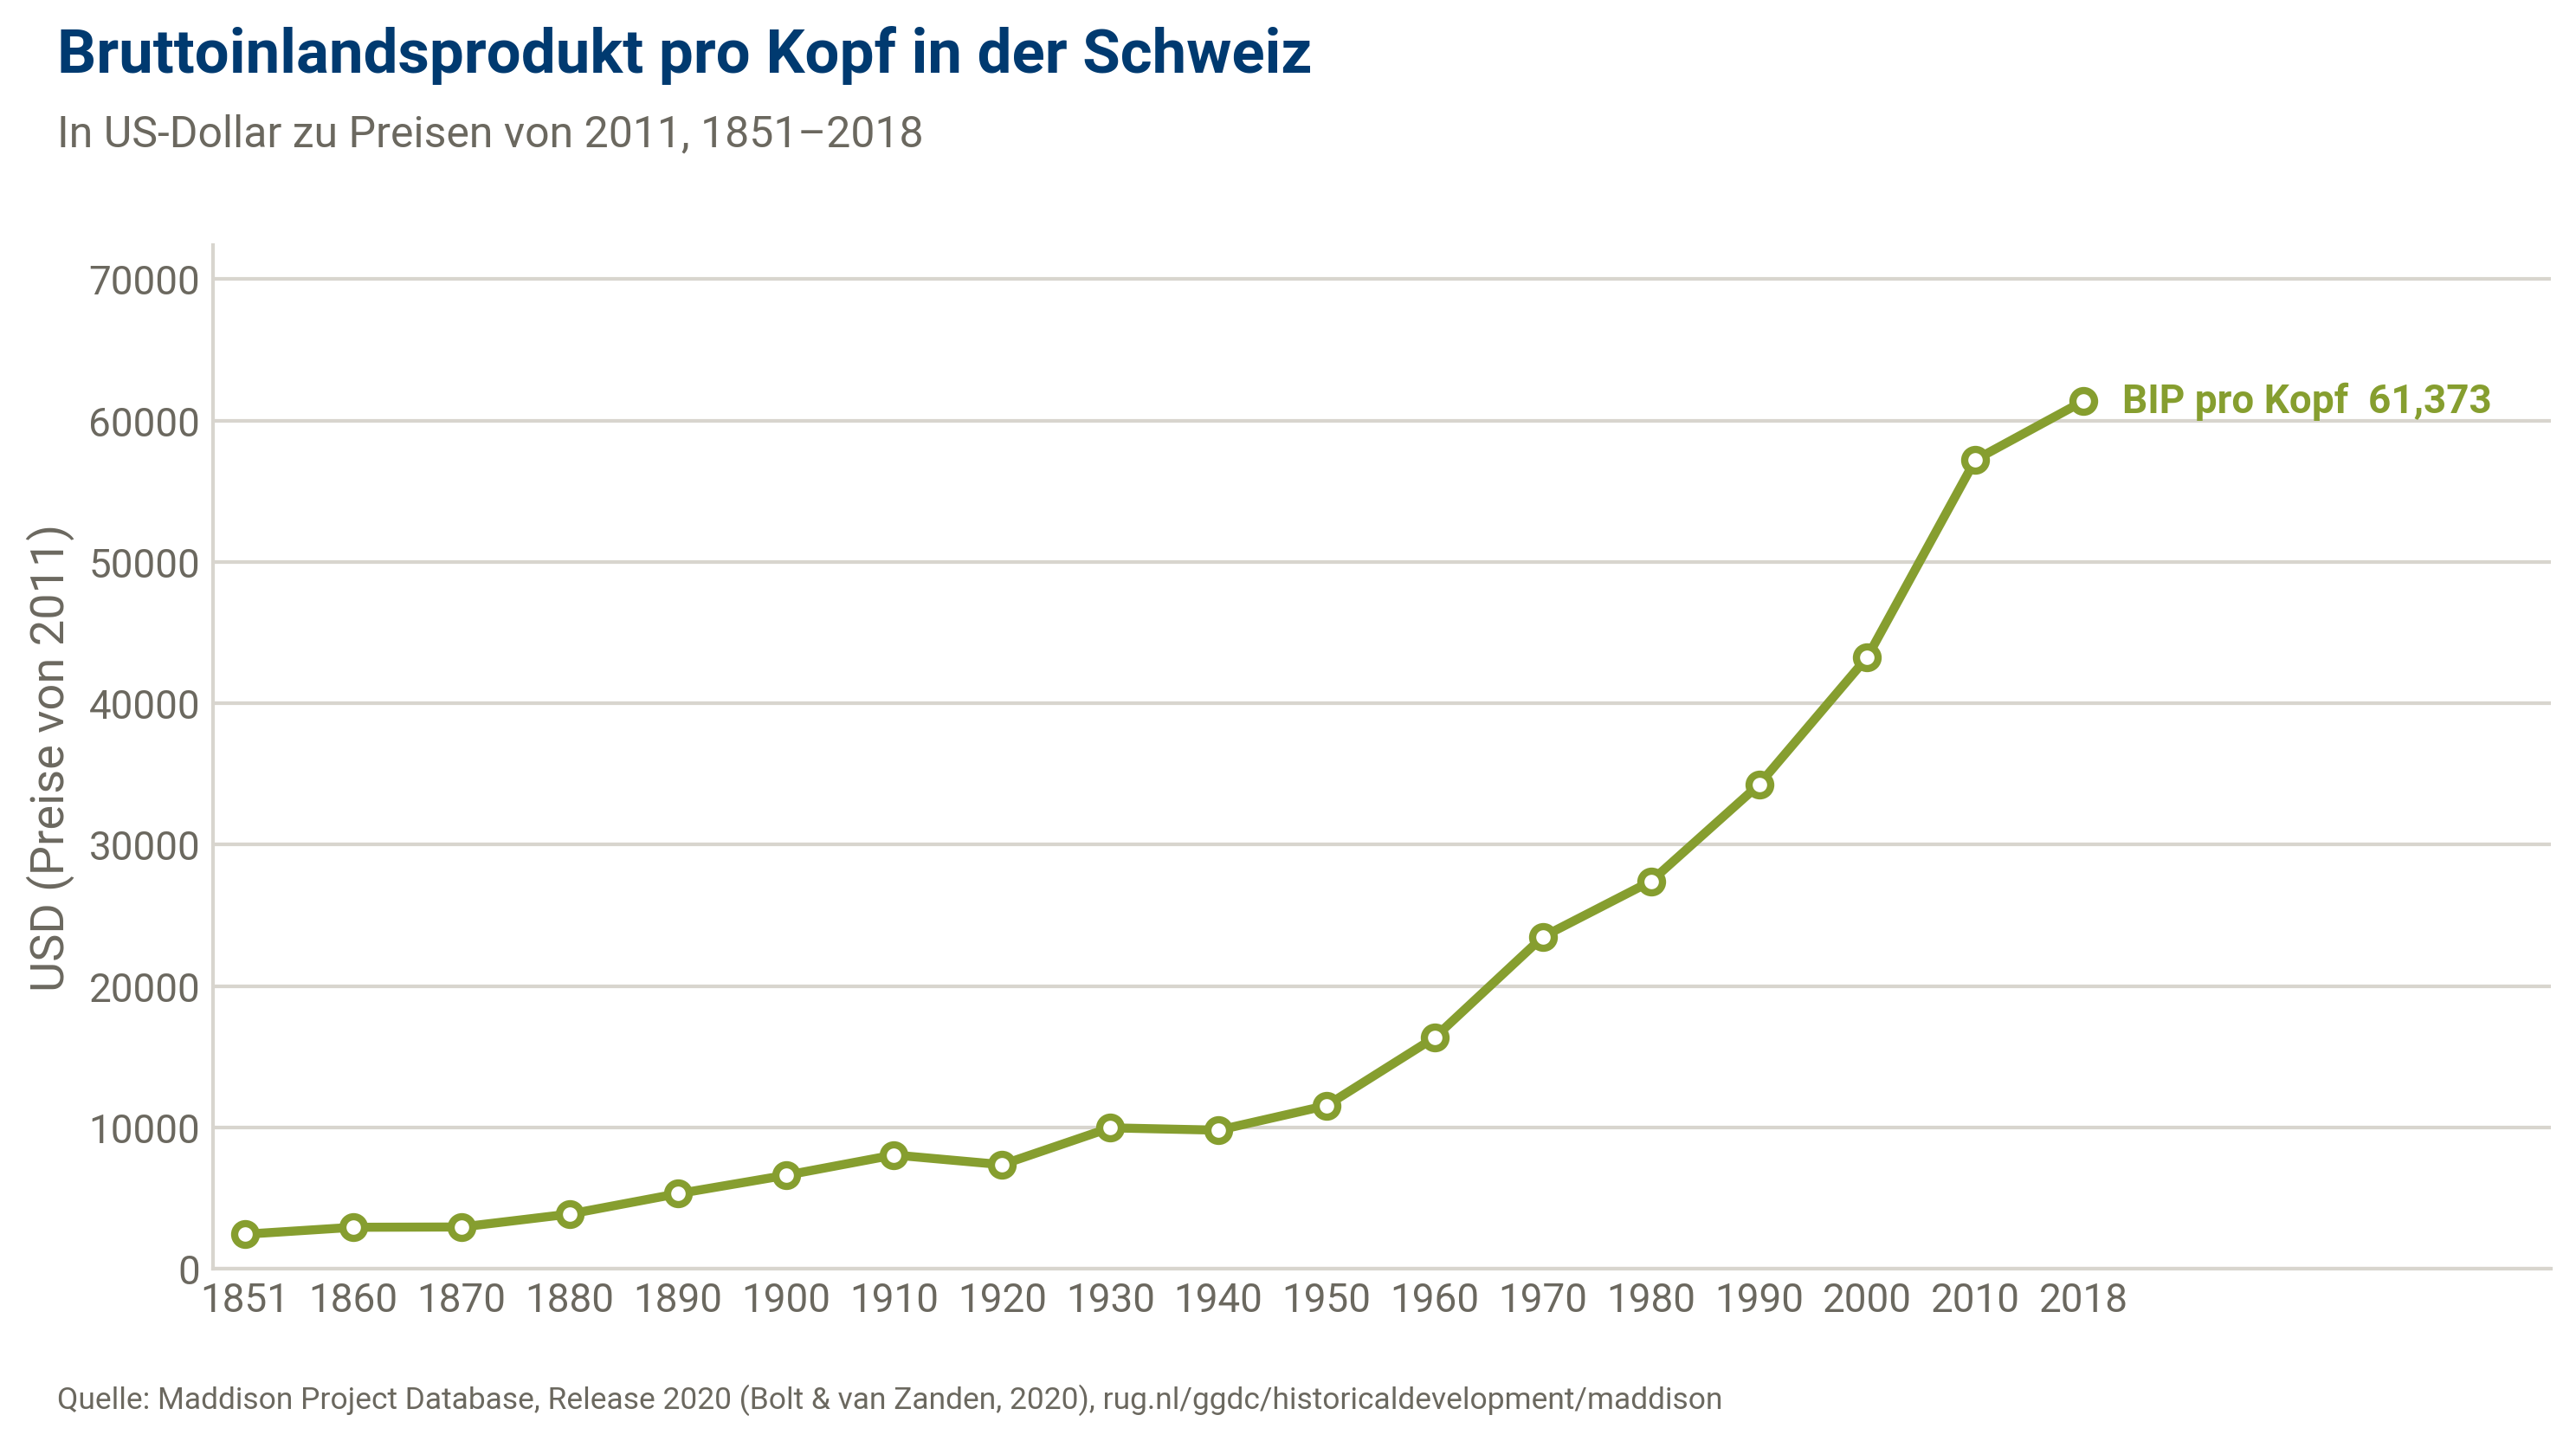
\includegraphics[keepaspectratio]{2_scope-of-economics/images/fig0.png}}

}

\caption{\label{fig-GDP-CH}Development of GDP per capita in Switzerland
at 2011 prices in USD. Source: Own illustration with data from The
Maddison Project (2020).}

\end{figure}%

\begin{figure}[H]

\centering{

\pandocbounded{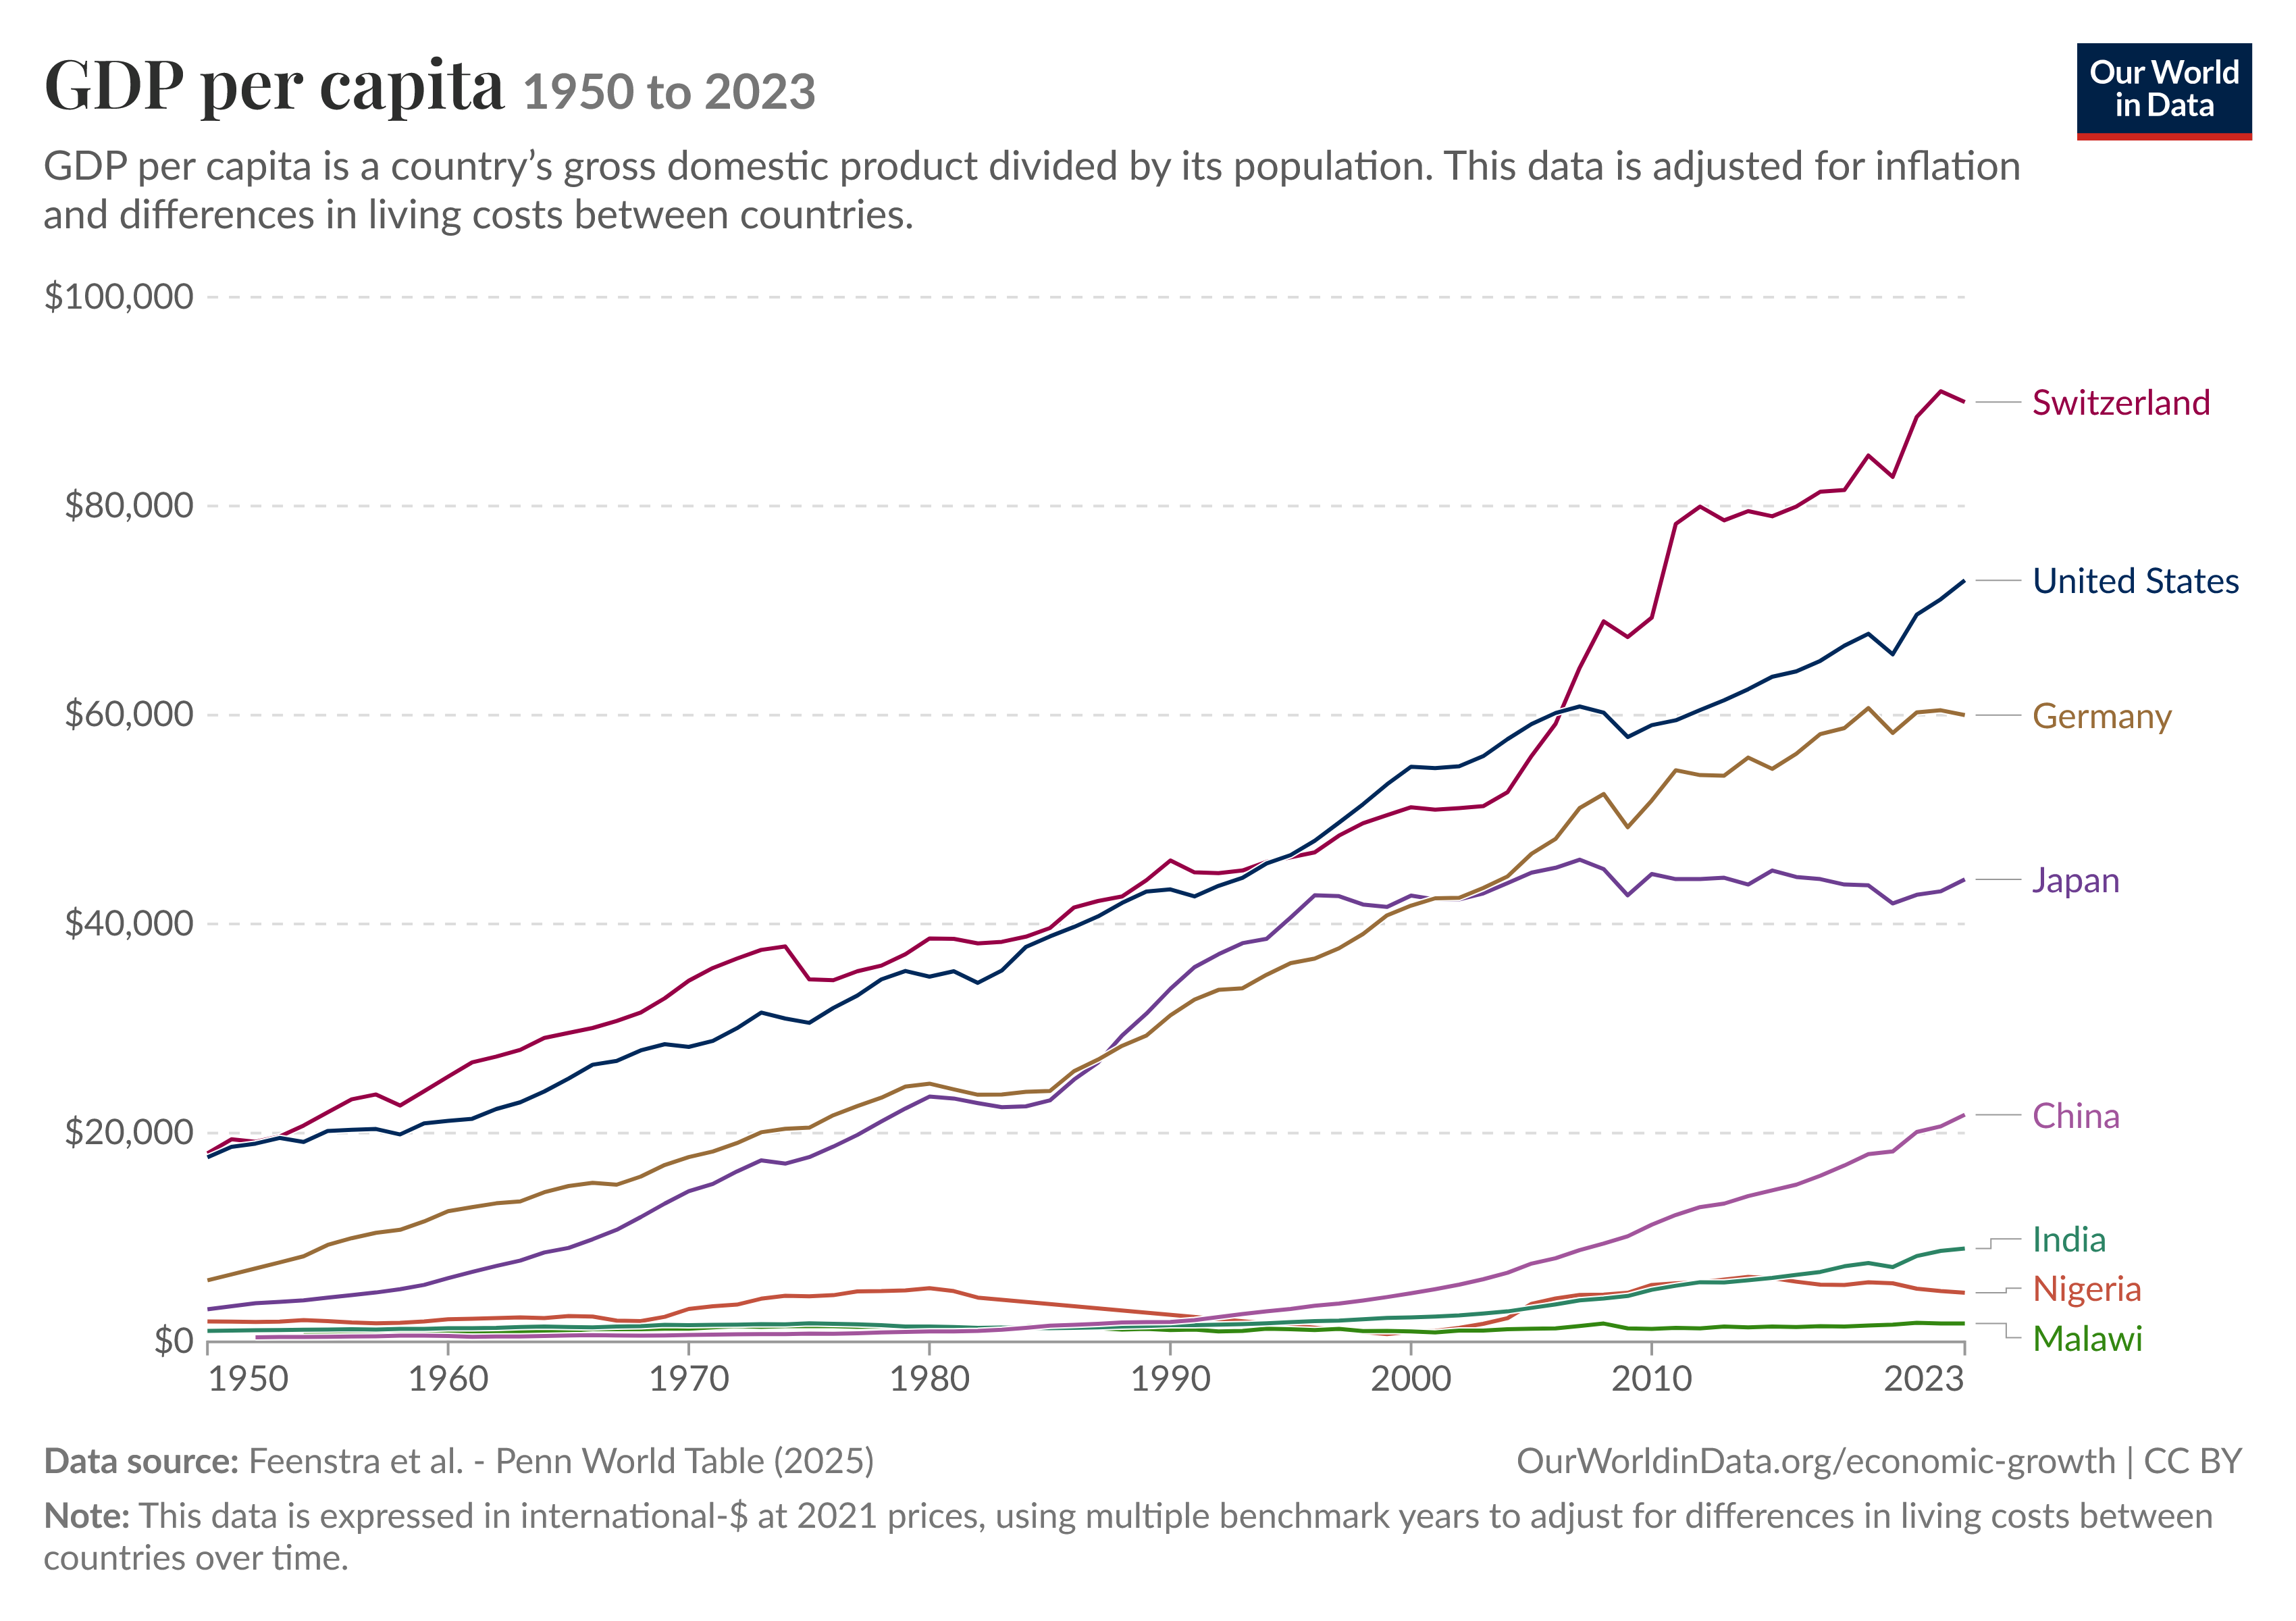
\includegraphics[keepaspectratio]{2_scope-of-economics/images/fig1.png}}

}

\caption{\label{fig-GDP-CH-comparison}GDP per capita of selected
countries, 1950-2023. Source: Feenstra et al.~-- Penn World Table (2025)
-- with extensive data processing by Our World in Data.}

\end{figure}%

\subsection{Alternative indicators of
prosperity}\label{alternative-indicators-of-prosperity}

If GDP screens out so many facets of prosperity -- how could prosperity
be captured instead? In view of the limitations mentioned, several
alternative indicators have been developed that aim to paint a more
comprehensive picture:

The \textbf{Human Development Index (HDI)} supplements GDP with life
expectancy and level of education. The HDI thus follows a concept of
prosperity and human well-being according to which people should be
enabled to lead a life worth living according to their own ideas. In
Chapter 3.2.2 (\emph{Justice and inequality}), we go into this approach
in more detail.

The \textbf{Genuine Progress Indicator (GPI)} goes further: besides
positive factors, it also includes negative ones such as environmental
pollution and social inequality -- in total about 26 indicators from the
economic, social, and ecological dimensions, including the value of
unpaid work.

Since it is fundamentally difficult or even impossible to measure
prosperity, these indicators, too, are criticized for their limitations,
and accordingly many further indicators exist for measuring a country's
prosperity. Besides GDP, however, none has so far been able to establish
itself.

\begin{figure}[H]

{\centering \pandocbounded{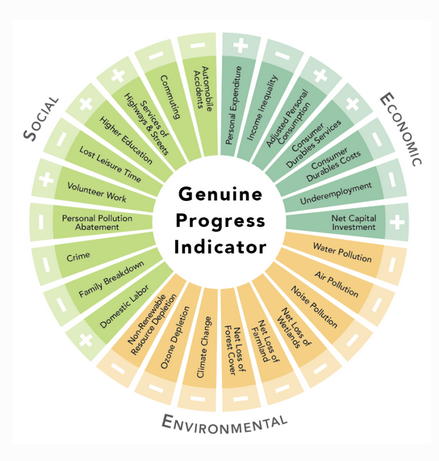
\includegraphics[keepaspectratio]{2_scope-of-economics/images/fig2.png}}

}

\caption{Aspects of the GPI. Source:
\href{https://gnhusa.org/genuine-progress-indicator/}{GNHUSA}.}

\end{figure}%

To illustrate how far different indicators can diverge,
Figure~\ref{fig-gpi-gdp} shows the calculations by Kubiszewski et al.
(2013) for the development of GDP and GPI per capita since the 1950s for
a group of 17 countries.

\begin{figure}[H]

\centering{

\pandocbounded{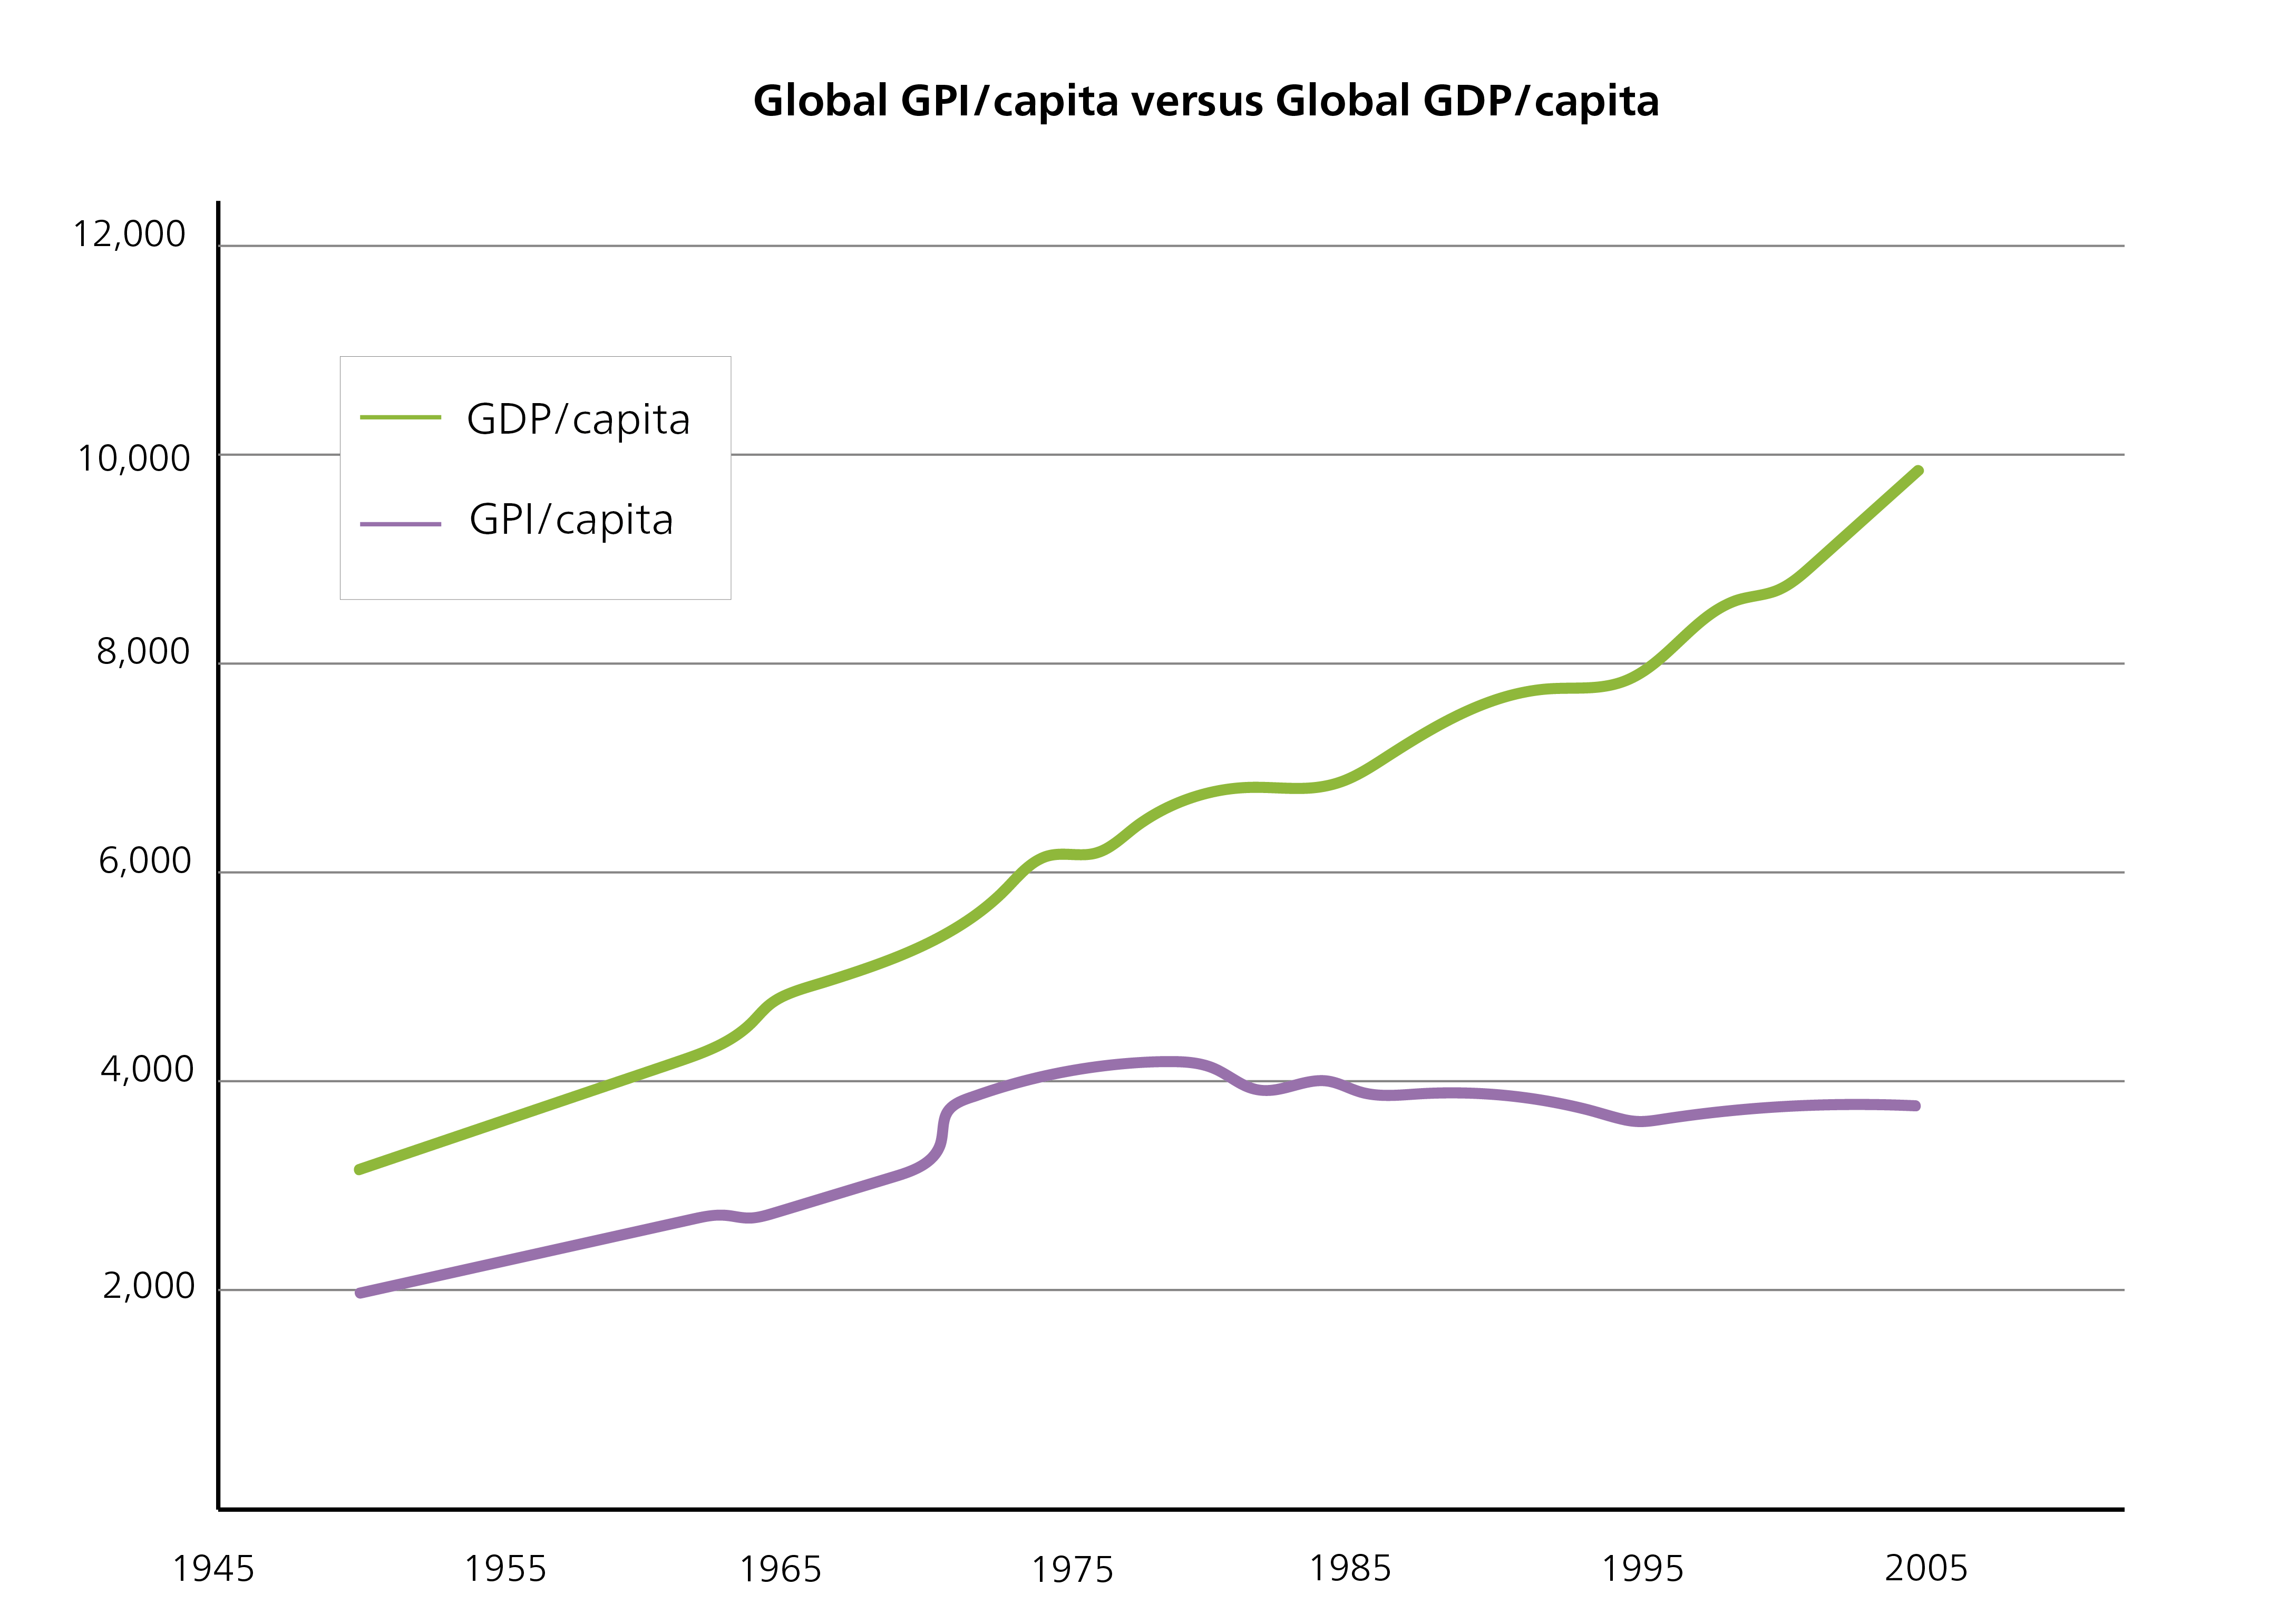
\includegraphics[keepaspectratio]{2_scope-of-economics/images/fig3.png}}

}

\caption{\label{fig-gpi-gdp}GPI vs.~GDP per capita. Source: Own
illustration with data from Kubiszewski et al. (2013, 63).}

\end{figure}%

\subsection{Economic growth}\label{economic-growth}

\emph{↗ Textbook chapter 4}

If prosperity is mostly measured by GDP, then the \emph{increase} in
this prosperity over time -- economic growth -- almost automatically
becomes the central political goal. Economic growth refers to the
increase in a country's economic output over time, usually measured by
the development of GDP. It is the central target variable for politics,
society, and the economy -- so central that Schmelzer and Vetter (2019,
62--68) speak of the \textbf{growth paradigm}.

Given this omnipresence of economic growth, it is astonishing that
economic growth is a very young phenomenon. Only with the Industrial
Revolution in England in the 19th century could sustained economic
growth (measured by GDP) be observed in the world for the first time.
For the longest part of human history, people lived without long-lasting
economic growth. Meanwhile, economic growth is not only a central
cornerstone of our current economic and social system but has developed
into a compulsion (Binswanger 2019). We will go into this systemic
growth imperative and the growth paradigm in more detail later in the
course. The significance of economic growth is intensively discussed
within sustainable economics, with positions that are far apart. While
some want to hold on to economic growth (in an adapted form), others
advocate overcoming economic growth as a compulsion (green growth
vs.~post-growth). At a later point, we will engage with these
discussions in depth.

Figure~\ref{fig-hockeystick} shows the development of GDP per capita for
different countries or regions over the last 1,000 years. The Industrial
Revolution in the 19th century is clearly visible.

\begin{figure}[H]

\centering{

\pandocbounded{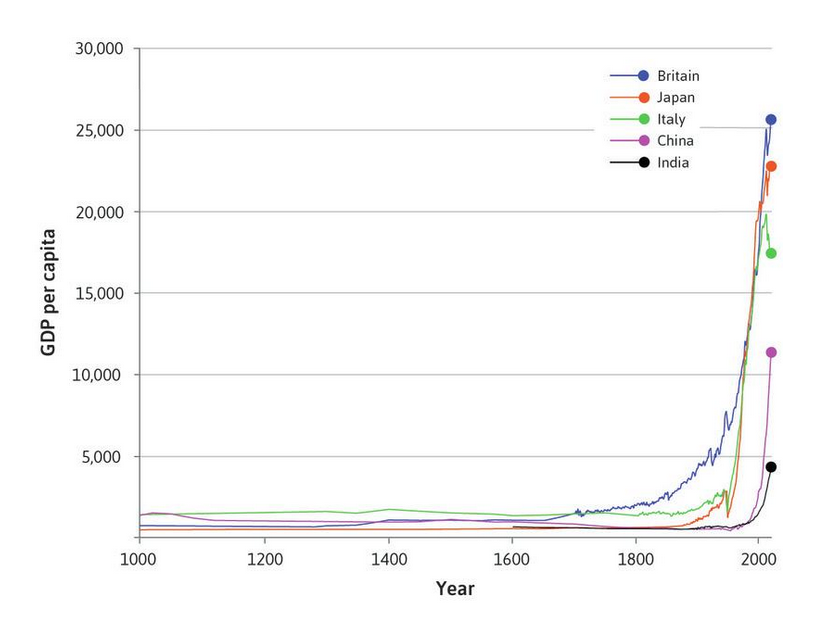
\includegraphics[keepaspectratio]{2_scope-of-economics/images/fig4.png}}

}

\caption{\label{fig-hockeystick}History's hockey stick: Gross domestic
product per capita in five countries (1000-2018). Per capita income
stagnated for centuries. Only with the Industrial Revolution and fossil
capitalism did incomes and production volumes rise exponentially --
albeit very unequally from region to region. Source:
https://books.core-econ.org/the-economy/microeconomics/01-prosperity-inequality-02-historys-hockey-stick.html\#figure-1-1.}

\end{figure}%

\begin{tcolorbox}[enhanced jigsaw, arc=.35mm, bottomrule=.15mm, bottomtitle=1mm, breakable, colback=white, colbacktitle=quarto-callout-note-color!10!white, colframe=quarto-callout-note-color-frame, coltitle=black, left=2mm, leftrule=.75mm, opacityback=0, opacitybacktitle=0.6, rightrule=.15mm, title={In-depth questions}, titlerule=0mm, toprule=.15mm, toptitle=1mm]

\begin{itemize}
\tightlist
\item
  Does GDP seem to you a sensible measure of a nation's prosperity? What
  speaks for it, and what against?
\item
  Think of examples from everyday life in which the growth paradigm can
  be recognized.
\item
  What could be the reasons that GDP and GPI diverge so strongly? And
  what could be the reason that the trends in the figure diverge only
  from the 1970s onwards?
\end{itemize}

\end{tcolorbox}

\begin{tcolorbox}[enhanced jigsaw, arc=.35mm, bottomrule=.15mm, bottomtitle=1mm, breakable, colback=white, colbacktitle=quarto-callout-caution-color!10!white, colframe=quarto-callout-caution-color-frame, coltitle=black, left=2mm, leftrule=.75mm, opacityback=0, opacitybacktitle=0.6, rightrule=.15mm, title={Further reading}, titlerule=0mm, toprule=.15mm, toptitle=1mm]

\begin{itemize}
\tightlist
\item
  Binswanger, Mathias. 2019. \emph{Der Wachstumszwang: warum die
  Volkswirtschaft immer weiterwachsen muss, selbst wenn wir genug haben}
  {[}The growth imperative: why the economy has to keep growing even
  when we have enough{]}. Wiley-VCH Verlag GmbH \& Co.~KGaA.
\item
  Lepenies, Philipp. 2013. \emph{Die Macht der einen Zahl: eine
  politische Geschichte des Bruttoinlandsprodukts} {[}The power of a
  single number: a political history of gross domestic product{]}. Erste
  Auflage, Originalausgabe. Suhrkamp.
\item
  Schmelzer, Matthias. 2016. \emph{The hegemony of growth: the OECD and
  the making of the economic growth paradigm}. Cambridge University
  Press.
\item
  Sen, Amartya. 2011. \emph{Development As Freedom}. Knopf Doubleday
  Publishing Group.
\end{itemize}

\end{tcolorbox}

\section{Forms of Provision in the
Economy}\label{forms-of-provision-in-the-economy}

\begin{tcolorbox}[enhanced jigsaw, arc=.35mm, bottomrule=.15mm, bottomtitle=1mm, breakable, colback=white, colbacktitle=quarto-callout-note-color!10!white, colframe=quarto-callout-note-color-frame, coltitle=black, left=2mm, leftrule=.75mm, opacityback=0, opacitybacktitle=0.6, rightrule=.15mm, title={Guiding question}, titlerule=0mm, toprule=.15mm, toptitle=1mm]

What is needed for prosperity -- as we discussed it in the last section
-- to arise in the first place?

\end{tcolorbox}

For a society to achieve prosperity, it must first ensure that goods and
services are provided at all. Through the division of labour, an
economic system always faces fundamental questions of organization: How
is societal production distributed? Who (re)produces, maintains, and
repairs what? Who consumes what? In other words: How is what is
necessary for prosperity produced in the first place and distributed
among the members of a society?

As became clear from the preceding chapters, the answers to these
questions depend strongly on which understanding of the economy one
takes as a basis. Here, we follow Karl Polanyi's (1957) substantivist
understanding, which defines the scope of the economy beyond the market
and proposes a broad understanding of the economy.

For our starting question -- what is needed for prosperity to arise --
Polanyi's broad substantivist understanding is particularly
illuminating. It shows that real economies consist of very different
institutions and logics. A housing cooperative works with different
business models than plumbers and steel companies, the public hospital
differs from the industrial firm, and unpaid care work is organized
differently from assembly-line work. Karl Polanyi therefore
distinguishes four socioeconomic organizing principles, or forms of
provision, that can be found in actually existing economies and interact
in different ways: householding, reciprocity, redistribution, and market
exchange (Polanyi 2017):

\begin{enumerate}
\def\labelenumi{(\arabic{enumi})}
\item
  \textbf{Householding} refers to forms of self-sufficiency and is
  rooted in families and households. In ancient Greece, the oikos, that
  is, the whole house, was an autarkic, that is, self-supplying,
  economic unit. But even today, a large part of the economy still takes
  place in the household, in particular as unpaid care, nursing, and
  childcare work as well as housework (for example cooking, cleaning,
  gardening).
\item
  \textbf{Reciprocity} is based on the principle of give-and-take and
  defines an exchange of goods and services between persons beyond the
  market and the state. On the one hand, it takes place in local
  communities and between persons who know one another, for example
  among friends, in the neighbourhood, or in associations, and includes,
  among other things, neighbourly help and community work. On the other
  hand, there are also many historical examples of reciprocal exchange
  over long distances, in which peoples exchange goods, with ceremonial
  motives and motives of maintaining relationships often playing a role
  alongside economic ones. To endure, however, this form of provision
  requires that giving and taking do not get too far out of balance or
  are underpinned by a corresponding ideal of justice (see Chapter
  3.2.2, \emph{Justice and inequality}).
\item
  \textbf{Redistribution} defines a systematic flow of resources towards
  an administrative centre and their subsequent redistribution. Examples
  are public education, health, and pension systems financed by taxes or
  levies. Redistribution allocates resources to members of a society
  (who are often unknown to one another). It takes place within
  political territories, in particular the nation-state, and therefore
  goes beyond local communities.
\item
  Finally, \textbf{market exchange} defines the exchange of goods and
  services at market prices. This is the commodified\footnote{Commodification
    means that something becomes a commodity and is traded on markets.
    That is, something is produced and distributed according to a market
    logic that previously did not work according to this logic (for
    example food produced for self-sufficiency). In principle, almost
    anything can be affected by commodification, for example labour,
    goods, natural resources, CO\textsubscript{2}, and so on. With the
    development of capitalism, more and more areas of the economy were
    commodified, which is why this appears self-evident to us in many
    areas.} area of economic activity. Depending on the type of goods
  and services traded and on their reach and structure, these markets
  can differ. The logic of individual profit and ability to pay
  predominates in market relations.
\end{enumerate}

\begin{tcolorbox}[enhanced jigsaw, arc=.35mm, bottomrule=.15mm, bottomtitle=1mm, breakable, colback=white, colbacktitle=quarto-callout-note-color!10!white, colframe=quarto-callout-note-color-frame, coltitle=black, left=2mm, leftrule=.75mm, opacityback=0, opacitybacktitle=0.6, rightrule=.15mm, title={In-depth questions}, titlerule=0mm, toprule=.15mm, toptitle=1mm]

\begin{itemize}
\tightlist
\item
  Find further examples from your everyday life for each form of
  provision.
\item
  Find an example of a good or service that is provided through all four
  forms of provision. How do the four forms of provision change the
  situation and the character of the transaction or provision?
\end{itemize}

\end{tcolorbox}

Back to the guiding question: prosperity thus does not arise through
market exchange alone. Real economies are always \textbf{mixed
economies}. They combine all four forms of provision, even if in
everyday life only market exchange is often perceived as ``the
economy''. Not every aspect of life and economic activity can -- or
should -- be turned into a marketable, commodified good. Which of these
forms of provision contribute how strongly to a society's prosperity
(and which of them become visible in classical prosperity measures such
as GDP) is thus itself a central economic question.

\section{(Re)production Factors}\label{reproduction-factors}

\emph{↗ Textbook chapter 16}

\begin{tcolorbox}[enhanced jigsaw, arc=.35mm, bottomrule=.15mm, bottomtitle=1mm, breakable, colback=white, colbacktitle=quarto-callout-note-color!10!white, colframe=quarto-callout-note-color-frame, coltitle=black, left=2mm, leftrule=.75mm, opacityback=0, opacitybacktitle=0.6, rightrule=.15mm, title={Guiding question}, titlerule=0mm, toprule=.15mm, toptitle=1mm]

What is needed for goods and services to come into being?

\end{tcolorbox}

To answer this question, economics needs a concept for the
``ingredients'' of economic activity: the \textbf{factors of
production}. Factors of production are all the inputs that are necessary
to produce an output -- a good or a service. The aggregated factors of
production of an economy are called \textbf{factor endowment}. The
origins of the factors of production lie in the physiocratic thinking of
the 18th century; as a concept, they became established in classical
economics. According to classical economics, the factors of production
of economic activity can be divided into three categories: \textbf{land,
capital, and labour.} Over time, this trinity has repeatedly been
criticized, extended, and adapted. Further factors such as
entrepreneurship, knowledge and technology, and nature itself, for
example, have been brought into play. Often, however, these aspects are
also subsumed under one of the three existing factors.

But the question ``What is needed for something to come into being?'' is
thereby only half answered. Many schools of thought (such as
neoclassical economics, post-Keynesian economics, and in part also
Marxist economics) focus above all on the \textbf{production} of goods
and services for sale on the market. What is often screened out is
\textbf{reproduction} -- that is, everything that is necessary for
something to continue to be usable. A bicycle, for example, has to be
pumped up regularly and its chain oiled so that it rides reliably. A cup
has to be washed thousands of times so that it can be used again. But
people, and thus workers, also have to be ``reproduced'' (this is often
described as social reproduction). We all need food, care, and so on in
order to live and to show up for work.

Whoever focuses only on production thereby screens out a central part of
what makes goods and services possible in the first place: unpaid
reproductive work such as cooking, cleaning, or childcare is often not
analysed but simply assumed as given. Feminist economics shows, however,
that this work is an integral part of economic life. It forms the basis
on which market-mediated activities can take place in the first place.
The separation into ``productive'' market-mediated work and
``unproductive'' housework, and its gender-specific connotations,
developed only with the emergence of capitalism and is by no means
natural. Questions of production and reproduction are thus also strongly
connected to the capitalist production system (see Chapter 2.5,
\emph{Abstract Markets or Capitalist Production System}).

In what follows, we turn to the three classical factors of production --
land, capital, and labour -- which, depending on the perspective, play a
central role not only for production but also for reproduction.

\subsection{Land -- can we replace nature with technology at
will?}\label{land-can-we-replace-nature-with-technology-at-will}

\emph{↗ Textbook chapter 13}

The factor of production land often covers not only the area or ground
itself but also the natural environment. The question is often how land
and natural resources are handled and how they are used. These questions
affect us very directly in everyday life. The design of living space,
for example, is of central importance for all of us. But how we deal
with agricultural land, forests, lakes, and the living beings within
them also plays a central role in our everyday lives. In addition, land
and natural resources are an elementary factor for the production of
goods and services. Land is indispensable for production, whether for
factories or agriculture. But natural resources such as water and rare
earths are also central as inputs for production.

What is special about land is that, on the one hand, it has unchangeable
natural characteristics (for example land is immobile and cannot be
multiplied), while, on the other hand, how it is handled is very
strongly socially determined (for example rights of ownership, access,
and use). This starting point means that the handling of land has a
great deal of conflict potential, is necessarily linked to questions of
distribution, and can also be an important aspect of inequality.
Accordingly, questions about the handling of land are deeply political.

\subsubsection{Perspective 1: Nature is replaceable in
principle}\label{perspective-1-nature-is-replaceable-in-principle}

Despite their vital importance, land and natural resources receive
little attention in economics. In many schools of thought such as
neoclassical economics or, in part, post-Keynesian theory, land is
either screened out, assumed, or treated as a pure asset (for example
housing) and thus subsumed under capital. In these theories, land very
rarely finds its way into production functions. And when land and
natural resources are explicitly considered, they are often understood
as ``ecological services'' (\emph{ecosystem services}). Through pricing,
they are then conceptualized as an input factor and commodity and
embedded in a market logic. In such understandings, land and natural
resources are thus implicitly or explicitly understood as ``pure input
factors'' and/or assumed as self-evident. A forest, for example, is
reduced to its purely economically exploitable dimension, such as the
sale of timber and game. What is often neglected is that nature is never
available in the form of goods but must always be made usable and
exploitable by humans through labour (Schaupp 2024). In these
understandings, it is also implicitly assumed that, for example, the
loss of biodiversity can be compensated by technological solutions. In a
cost-benefit analysis, all costs and benefits are then summed up, and
all the different aspects are thus equated through monetary valuation.
For sustainable economics, such fundamental questions are of central
importance. In addition, through the reference to market logic,
questions of land are depoliticized, and questions of power and
distribution are implicitly excluded.

\subsubsection{Perspective 2: Nature has limits that technology cannot
lift}\label{perspective-2-nature-has-limits-that-technology-cannot-lift}

In contrast, there is a fundamentally different understanding of land
and natural resources as non-replaceable goods that form the basis of
social life. In this understanding, the loss of biodiversity or the
destruction of fertile soil cannot be compensated. These losses are
final. Such understandings often come from ecological economics, but
some currents of feminist and Marxist economics also build on this
understanding. The natural limitedness and the need for social
organization in dealing with land are taken as the starting point, and
questions of power and distribution are often made explicit.

Whether nature can be replaced by technology at will is thus not a
purely technical question but a theoretically and politically charged
one. In Chapter 3.1, we go deeper into different understandings of
nature and their consequences. What is important to take away here above
all is that land, and its significance for economic life, can be
understood and conceptualized in different ways. In addition, land and
natural resources have some unchangeable, natural characteristics. Who
has access to them, however, is not subject to any natural economic law
but is the result of economic, political, and social structures.

\subsection{Capital -- why do some people own capital and others do
not?}\label{capital-why-do-some-people-own-capital-and-others-do-not}

\emph{↗ Textbook chapter 11}

We encounter capital every day in various forms, yet the term mostly
hides in rather technical vocabulary. With a certain amount of start-up
capital, for example, we can found a company, invest money in a capital
investment (for example buying securities), or invest in our own
education, which is referred to as human capital. Not least, our
economic system -- capitalism -- is named after the (company) capital
that empowers its owners to make the decisions that matter for the
company. Accordingly, it must play an important role. But what exactly
is it? The examples given already show that an important aspect is that
one invests (in) something that is later supposed to yield a return (a
\emph{capital} return): by investing start-up capital, I want to build a
company that later makes profits, the purchase of securities is supposed
to yield regular interest, and the investment in education is supposed
to pay off through a higher wage in working life. But do these examples
all refer to capital to the same extent, or are there differences?
Again, this question is answered differently depending on the
perspective.

\subsubsection{Capital as a thing -- inequality as the result of
different
investments}\label{capital-as-a-thing-inequality-as-the-result-of-different-investments}

Neoclassical economics sees capital first and foremost as a factor of
production, that is, mainly machines, tools, factory buildings, and so
on. With this (physical) capital, goods are then produced with the help
of labour as the second factor of production. On the capital market (or
the market for financial capital), the rate of return is then
determined, which in equilibrium corresponds to the productivity of
physical capital. Capital is understood here primarily as a commodity
that is traded on a market and valued and distributed according to
market mechanisms. The main thought here is of the production of goods,
but in this understanding human capital can very well also be understood
as such. I invest time and forgo wages during my training and then
expect a return in the form of a higher wage, which is regulated through
the market mechanism.

This understanding fits our guiding question as follows: whoever owns
more capital has invested (or inherited) more in the past. Inequality
therefore appears here primarily as the result of different investment
decisions and opportunities, not as a structural problem. To distinguish
it from money: \textbf{money} can also be capital in this understanding,
provided it is invested in order to achieve a return -- money that
merely lies in a drawer would, strictly speaking, not be capital.

\subsubsection{Capital as a social
relation}\label{capital-as-a-social-relation}

Post-Keynesian theory, too, understands the concept of capital primarily
as a factor of production but connects entirely different dynamics with
it (see Chapter 2.5). In particular, a concept of capitalism and the
distinction of classes are connected with it: workers who have no
capital and therefore have to work for their wages, and capitalists who
have capital and can deploy it to make profits. Questions of power and
distribution thus also increasingly come into view.

Post-Keynesian economics took this view of the relationship between
classes from Marxist economics. Marxist economics makes this relational
aspect of capital the central point: capital here is not a thing but a
\textbf{social relation}. The deployment of capital is based on the
separation of the means of production from the workers, who have to work
for a wage -- that is, sell their labour power, since they themselves
have no capital. In this understanding, we do not speak of capital, for
example, in the case of machines used for agricultural self-sufficiency.
But if an entrepreneur buys machines and pays wage workers to till the
land for them, and the harvest is sold on the market to make a profit,
we speak of capital in this understanding. Capital is thus tied to the
use of wage labour to make a profit, and this class relation is the
central aspect of capital. The Marxist concept of capital is accordingly
tied to the specific context of capitalism and cannot be extended at
will to other times or contexts. The concept of human capital, too,
makes little sense in this understanding. The capitalist dynamic that
capital must constantly multiply (accumulation) is likewise already
inherent in this concept as a social relation. In our example, the
entrepreneur would then, for example, invest the profit made in further
machines to expand production. This dynamic would then continue
steadily.

To distinguish it from money: mere money is not yet capital in this
understanding. Only when it is deployed to mobilize wage labour and make
a profit from it does it become capital. Hodgson (2014) therefore also
finds this understanding insufficient and understands capital as
everything that can potentially be used to make a profit. Concretely,
this means that all wealth is understood as capital, provided it can
also serve as collateral for taking out loans. This understanding of
capital also underlies, for example, Piketty's analysis in his major
work \emph{Capital in the Twenty-First Century} and can be connected
with various schools of thought (Piketty and Goldhammer 2014).

Although public debates often act as if it were entirely clear what is
meant by ``capital'', quite different understandings appear here -- and
with them different answers to our guiding question. Whether inequality
in capital ownership is understood as the result of individual
decisions, as a structural power relation, or as a self-reinforcing
wealth advantage depends on which concept of capital we take as a basis.
It is therefore central to be aware of which concept of capital we use
and for what purpose.

\subsection{Labour -- why do I earn as much as I do -- and why is some
work, such as care work, often not paid at
all?}\label{labour-why-do-i-earn-as-much-as-i-do-and-why-is-some-work-such-as-care-work-often-not-paid-at-all}

\emph{↗ Textbook chapter 12}

Labour is the third factor of production and is necessary so that goods
and services can be obtained from raw materials. Coordinating, mental,
and executing activities are necessary for the purposeful use of capital
in order to be able to produce. Labour is thus a central factor for
value creation. In many cases, labour also determines people's everyday
lives and takes a central role in economic policy reporting, for example
through discussions of unemployment, employment figures, and minimum
wages. This often concerns a specific form of labour: \textbf{paid
employment.}\footnote{Paid employment means activities for which people
  receive a direct return in the form of money.}

This is precisely where our guiding question comes in: Why do some
people earn a lot for their work and others little -- and why does some
work count as worthy of payment at all, while other work, such as care
and nursing work, often remains unpaid? As we will see, the answer
depends strongly on which economic understanding of labour one follows.

\subsubsection{Centrality of paid employment -- what counts as work at
all}\label{centrality-of-paid-employment-what-counts-as-work-at-all}

In our everyday lives, too, much revolves around paid employment. But
this centrality of paid employment developed only in the course of
19th-century industrial capitalism and became the central societal
instance of integration and orientation. While in premodern household
economies paid and unpaid activities were closely connected and the
household was the central economic unit, now only market-mediated,
remunerated labour was increasingly recognized as productive, while care
and housework were devalued. With the development of capitalism, more
and more people became dependent on paid employment to make a living.
And the capitalist system, too, depends on paid employment, since
excessively high unemployment can weaken economic development and lead
to a societal crisis (post-Keynesians emphasize that with low
employment, aggregate demand also falls away). In addition, social
security and tax revenues were built strongly on paid employment, and
societal participation and social recognition also orient themselves
towards paid employment. In the second half of the 20th century, this
development was consolidated by the idea of the \emph{standard
employment relationship} and the male breadwinner as a societal guiding
model.\footnote{Following Bernet (2021, 128), the term ``standard
  employment relationship'' is understood as a ``permanent, socially
  insured, and collectively protected full-time position with a secure
  monthly income, clearly regulated working hours, protection against
  dismissal, and certain instruments of co-determination'' {[}our
  translation{]}. Despite its name, this employment relationship was
  never really normal. There were always many people who did not work
  under such conditions, very often migrants and women.}

Since the 1970s, this model has come under increasing pressure, in
Switzerland too, through the flexibilization and precarization of
employment (for example the gig economy). Since the 1970s, unemployment
and underemployment have risen in Switzerland, as have temporary work,
part-time employment, and precarious and informal employment (Benelli
and Streckeisen 2014; Halbeisen et al. 2012; Sheldon 2007; Scherschel et
al. 2012; Baumgartner et al. 2019). Over the last 50 years, women have
also increasingly entered the labour market but mainly work part-time.

In line with the centrality of paid employment, many schools of thought
-- such as neoclassical and post-Keynesian economics -- focus strongly
on paid employment, while unpaid reproductive work is mostly tacitly
assumed. Feminist economics, by contrast, works with a considerably
broader concept of labour that also includes unpaid work. It often draws
on the so-called \textbf{third-person principle}: any activity that
could in principle also be performed by a third, paid person counts as
work. Cooking, cleaning, or childcare, for example, thus fall under
``work'' just as much as factory work, regardless of whether they are
remunerated or not.

Feminist economics also points out that person-related services (for
example nursing, care) follow a different logic than, say, factory work.
Unlike factory work, the productivity or efficiency of person-related
services can hardly be increased, because the quality of the work
depends directly on time and human interaction and can therefore hardly
be standardized or planned. As a result, wage costs in these areas rise
relative to other sectors, since they cannot (for example through new
technologies) show ever higher labour productivity, while wages rise
with societal development. The economist William Baumol described this
under the term \emph{cost disease} and shows how, for example, costs in
technological sectors have fallen massively while they continue to rise
in person-related services. In Switzerland, this is clearly visible, for
example, in the health-care system, where costs rise, calls for
efficiency improvements arise but cannot be implemented, which puts
staff under great pressure.

\subsubsection{But how are working time and wages
determined?}\label{but-how-are-working-time-and-wages-determined}

This brings us to the core of the guiding question: Why do \emph{I} earn
as much as I do? Here, too, the schools of thought diverge. Neoclassical
economics sees the central explanation in the market mechanism of the
labour market: in equilibrium, the wage corresponds to labour
productivity. People maximize their personal utility by deciding,
according to their preferences, on an optimal ratio between leisure and
consumption, which is made possible by selling labour (time). Whoever
wants to work finds work in this model too: in market equilibrium, there
is no (involuntary) unemployment. From this perspective, one thus earns
what corresponds to one's own productivity.

Feminist, post-Keynesian, and Marxist economists contradict this:
because of the societal centrality of paid employment, people are
ultimately compelled to work and cannot freely determine their working
time. Power imbalances in the labour market and institutions such as
trade unions play a central role in this process. In addition, feminist
economics emphasizes that these questions are also often shaped by
societal norms, so that the distribution of work, working time, and
wages is also co-determined by questions of gender.

\subsubsection{Unemployment}\label{unemployment}

In line with the centrality of paid employment, often only figures on
paid work are recorded and included in analyses. The most important
indicator used is usually the \textbf{registered unemployment rate}.
This is mostly calculated as follows:

\[\text{Unemployment rate} = \frac{\text{Number of registered unemployed}}{\text{Labour force}}\]

This indicator is only one of several indicators that are used, however.
The International Labour Organization (ILO), for example, relies on
unemployment in the ILO sense and, accordingly, the ILO unemployment
rate (\emph{Erwerbslosenquote}) as an indicator. All persons of the
permanent resident population in Switzerland who are without work, are
looking for a job, and could start an activity within a short time count
as
\href{http://www.bfs.admin.ch/bfs/de/home/statistiken/arbeit-erwerb/erhebungen/els-ilo.html}{\textbf{unemployed
according to the ILO}}.
\href{https://www.admin.ch/de/newnsb/yFqP7XwYSs3ODBR8ZdR9g}{In 2025, the
registered unemployment rate in Switzerland averaged 2.8\%}, and the
\href{https://www.bfs.admin.ch/bfs/rm/home/statisticas/catalogs-bancas-datas.assetdetail.36326600.html}{seasonally
adjusted ILO unemployment rate in the fourth quarter of 2025 was 5.0\%}.
Unlike the registered unemployment rate, the ILO unemployment rate also
includes, for example, self-employed persons, persons affected by
long-term unemployment such as those whose benefits have run out, and
young people who are not yet in gainful activity directly after their
training. Accordingly, the ILO unemployment rate is higher than the
registered unemployment rate. Such indicators say nothing about the type
of employment and employment relationships, however, so they are not
useful for such an assessment. More fundamental questions about the
meaning and purpose of work and of a high-employment goal also cannot be
discussed with such indicators.

As with questions about working time and wages, the schools of thought
also see different reasons for unemployment. In neoclassical economics,
unemployment is interpreted above all as the result of market
disturbances or market failure, that is, when certain factors disturb
the frictionless functioning of the market mechanism. A classic example
of such ``market disturbances'' is minimum wages above the market
equilibrium, which raise costs for companies and thus lead to
unemployment. If there are no disturbances in the market mechanism,
there is in principle no (involuntary) unemployment. Post-Keynesian
economics emphasizes above all that unemployment does not arise from the
labour market but depends on economic development and aggregate demand.
If the latter falls, no more people are hired or employees are
dismissed, and unemployment rises. It also emphasizes, however, that
full employment is not necessarily desired by employers, since a certain
level of unemployment also strengthens companies' bargaining power
(Kalecki 1943). Marxist economics, too, emphasizes that unemployment is
a structural part of capitalism and strengthens the bargaining power of
capital vis-à-vis employees (Magdoff and Magdoff 2004). Feminist
economics emphasizes that unemployment is not gender-neutral and that
women are more often part of the hidden reserve who would like to do
more paid work, or any paid work at all, but cannot, for example because
of unpaid care work.

The following figure shows the development of the unemployment rate in
Switzerland since 1920. Unemployment was and is very low in Switzerland
in international comparison. Especially during the post-war economic
boom, there was almost no unemployment in Switzerland, which is why
Switzerland brought in many workers from abroad -- who often worked
under precarious conditions (Halbeisen et al. 2012). Only with the
crisis of the 1970s did unemployment return to Switzerland, although
Switzerland prevented a sharp rise by exporting unemployment abroad --
by 1977, almost 250,000 foreign workers had to leave the country
(Halbeisen et al. 2012, 910).

\begin{figure}[H]

{\centering \pandocbounded{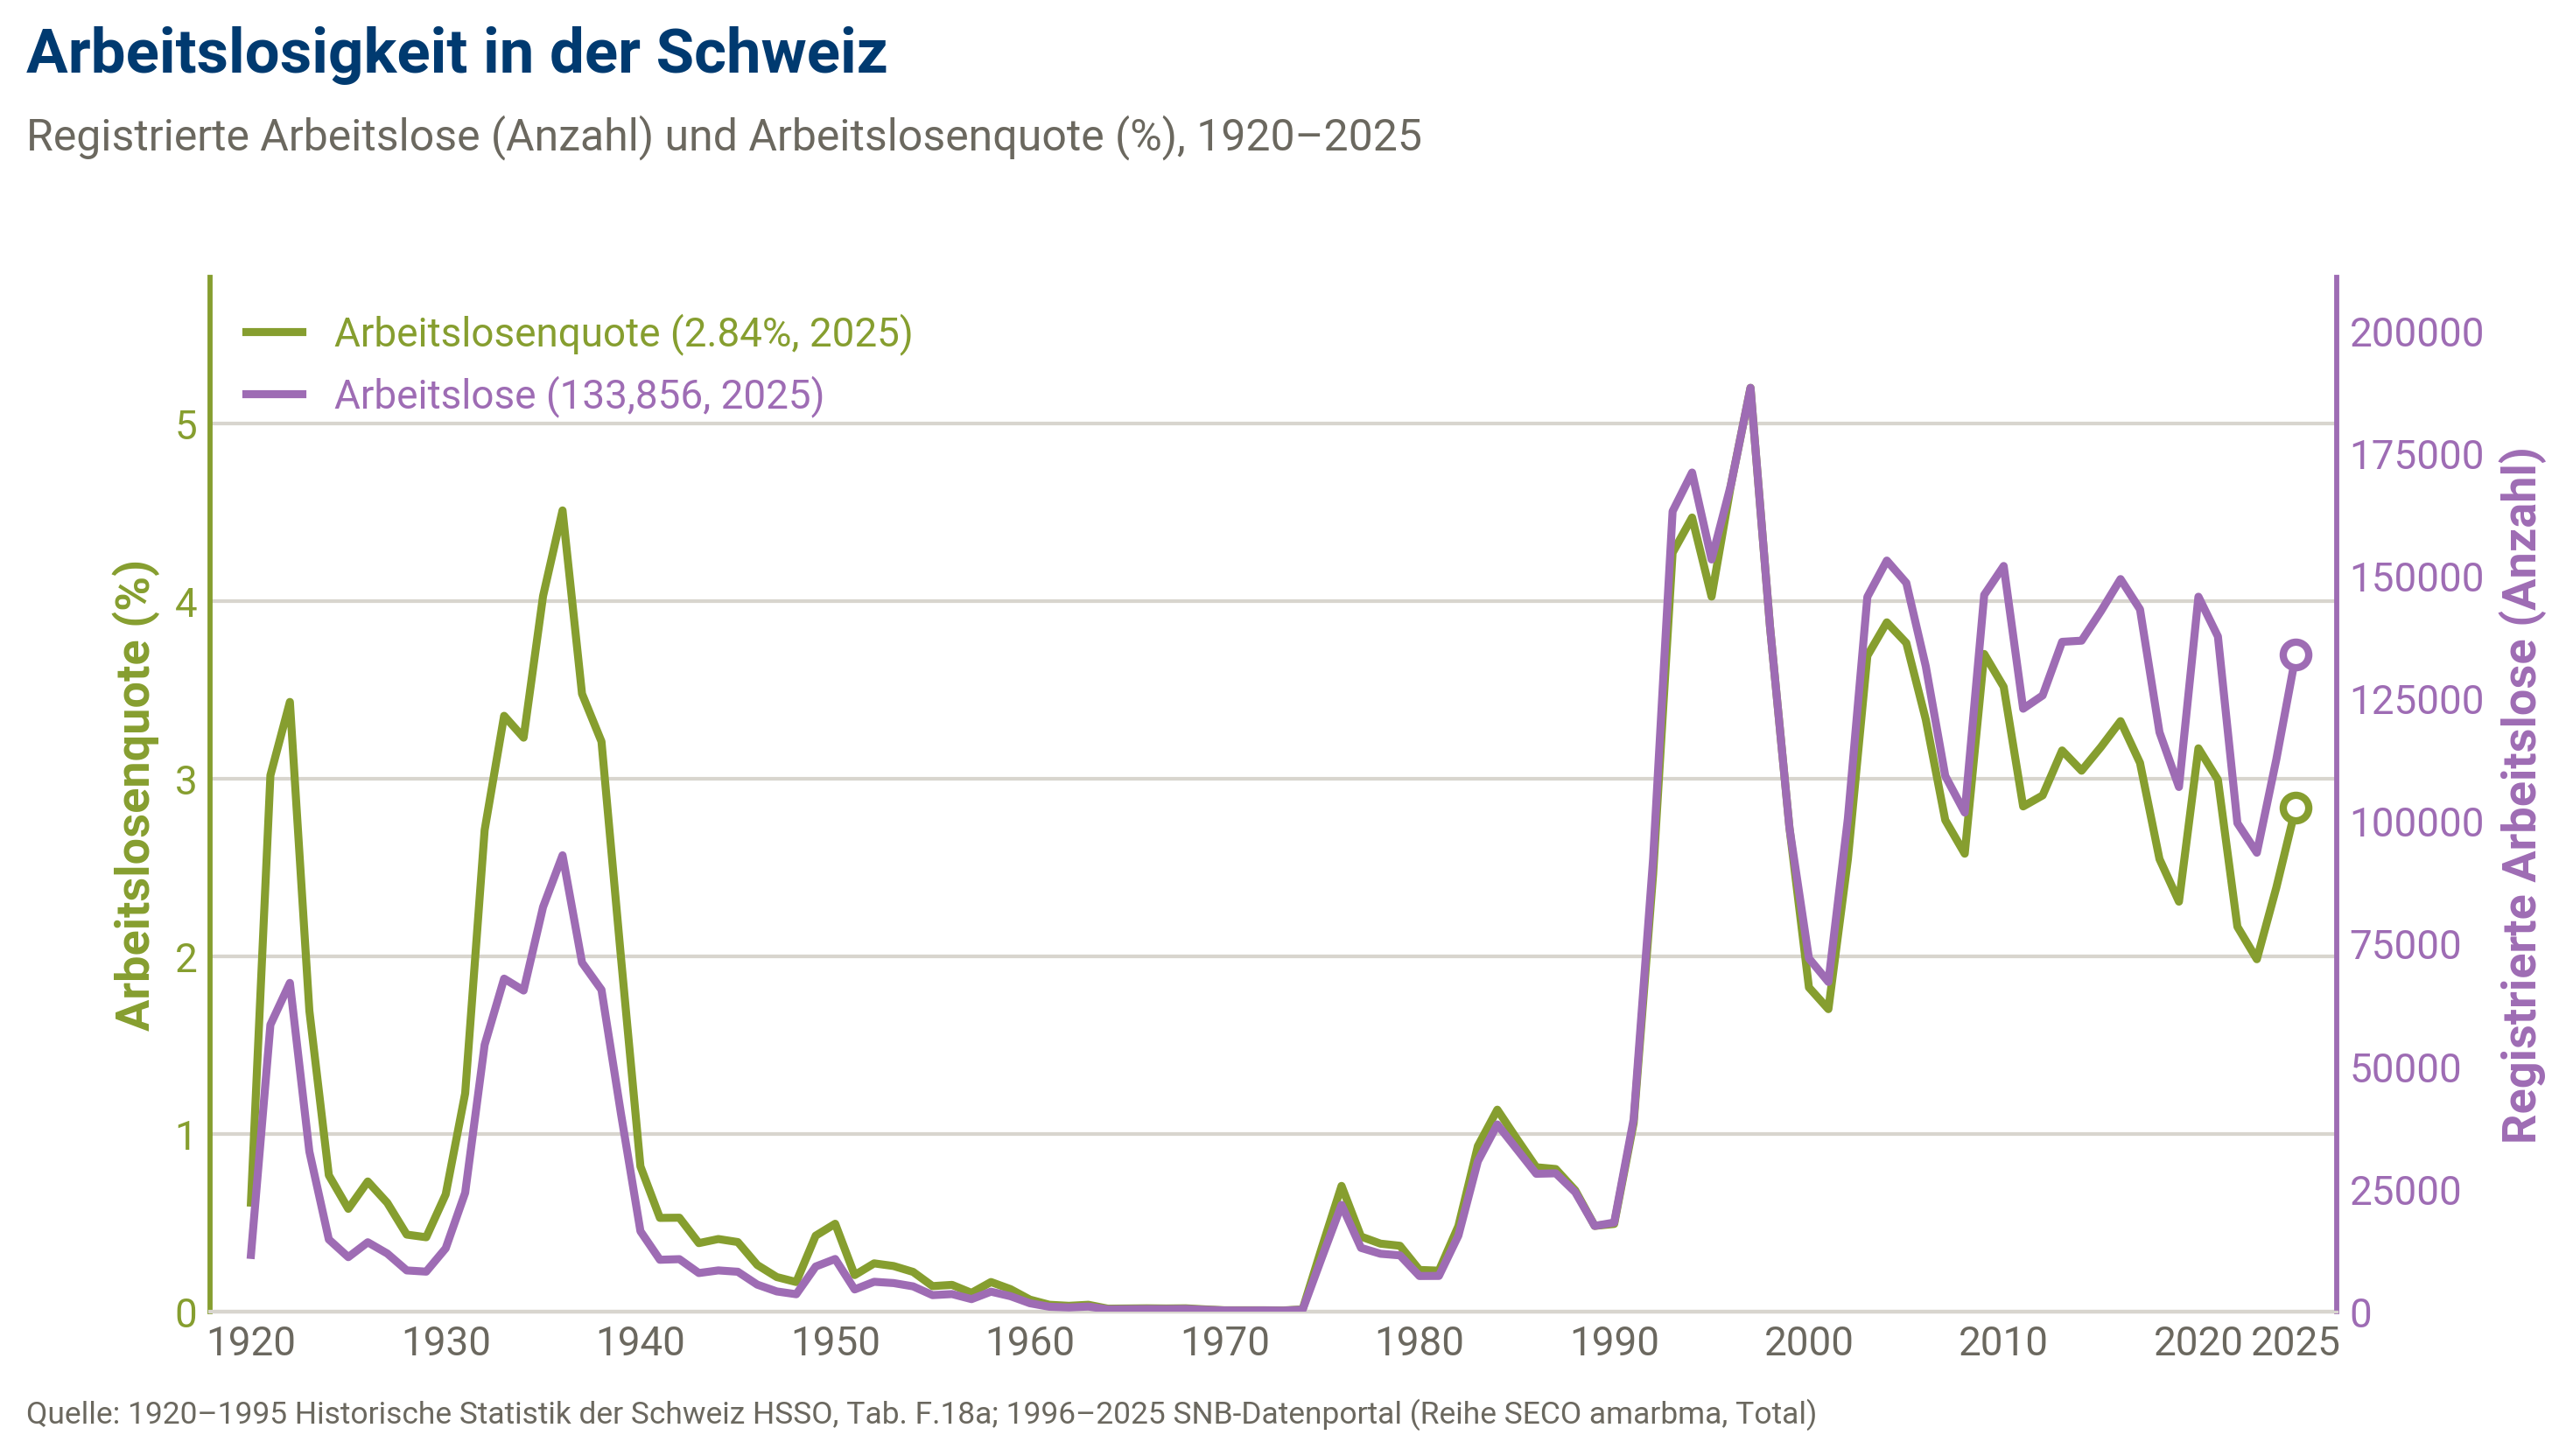
\includegraphics[keepaspectratio]{2_scope-of-economics/charts/figure11-unemployment-rate-switzerland/figure11-unemployment-rate-switzerland.png}}

}

\caption{Unemployment in Switzerland 1920-2025. Source: Own illustration
based on data from the Statistical Yearbook of Switzerland (1920-1996)
and from SECO (1997-2019).}

\end{figure}%

\subsubsection{Unpaid work}\label{unpaid-work}

Since 1997, the Federal Statistical Office (FSO) has recorded the
monetary value and the quantity of unpaid work in Switzerland every four
years with the household production satellite account
(\href{https://www.bfs.admin.ch/bfs/de/home/statistiken/arbeit-erwerb/erwerbstaetigkeit-arbeitszeit/vereinbarkeit-unbezahlte-arbeit/satellitenkonto-haushaltsproduktion.html}{SHHP}).
In Switzerland in 2020, 9.8 billion hours were worked unpaid (mostly by
women), more than were spent on paid work (7.6 billion hours). All
unpaid work in 2020 is estimated at a value of CHF 434 billion. If GDP
is extended by total household production, the latter corresponds to
41.4\% of the value added of the extended total economy.
Figure~\ref{fig-unpaid-paid} shows how paid and unpaid work are
distributed between the genders. Overall, women perform somewhat more
working hours per week than men; the big difference is that the majority
of these are not paid.

\begin{figure}[H]

\centering{

\pandocbounded{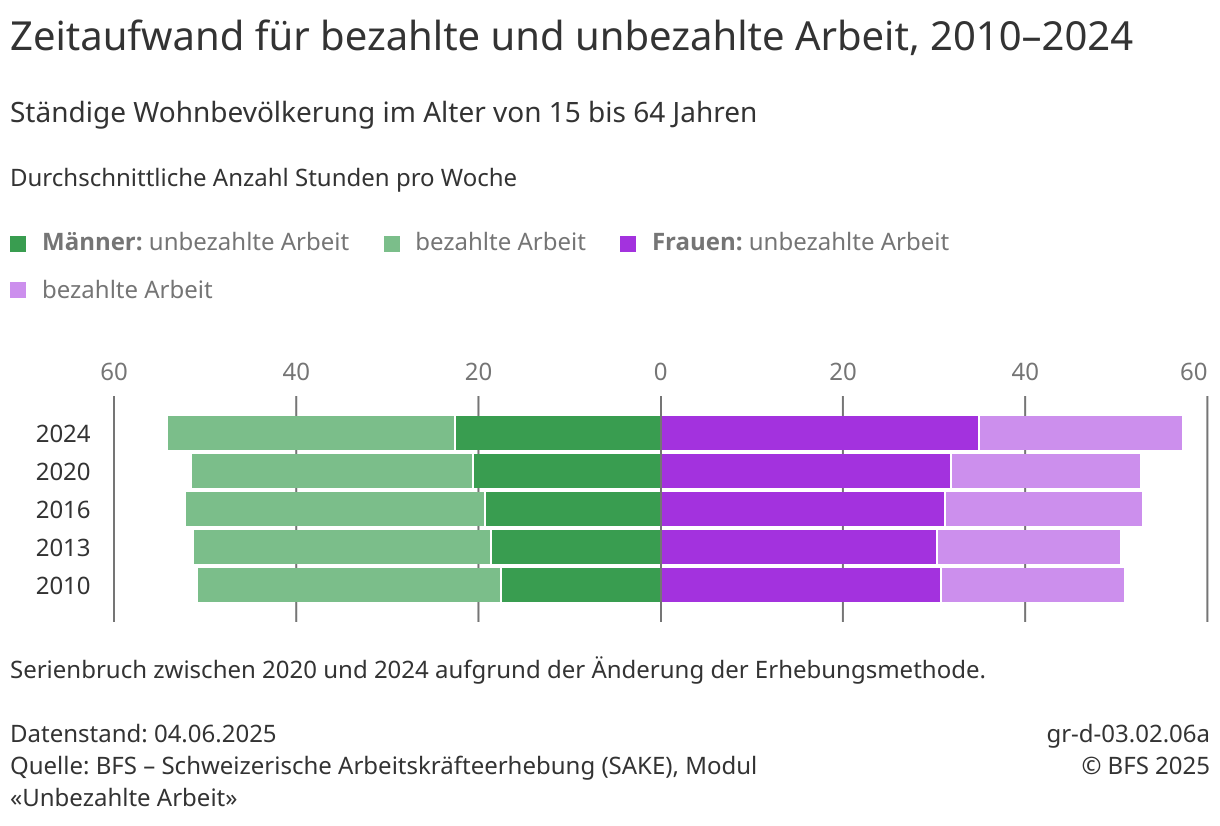
\includegraphics[keepaspectratio]{2_scope-of-economics/images/fig5.png}}

}

\caption{\label{fig-unpaid-paid}Time spent on paid and unpaid work,
2010-2024. Source: FSO
(https://www.bfs.admin.ch/bfs/de/home/statistiken/arbeit-erwerb/erwerbstaetigkeit-arbeitszeit/vereinbarkeit-unbezahlte-arbeit.html).}

\end{figure}%

The question ``Why do I earn as much as I do?'' thus cannot be answered
by individual productivity alone. It depends on which activities count
as ``work'' at all, on how bargaining power and institutions shape the
labour market, and on which historically grown norms determine whose
work is visible and remunerated. Care work often remains unpaid -- not
because it would be less necessary, but because our present notion of
``productive'' work is historically tied to the rise of paid employment
in capitalism.

\begin{tcolorbox}[enhanced jigsaw, arc=.35mm, bottomrule=.15mm, bottomtitle=1mm, breakable, colback=white, colbacktitle=quarto-callout-note-color!10!white, colframe=quarto-callout-note-color-frame, coltitle=black, left=2mm, leftrule=.75mm, opacityback=0, opacitybacktitle=0.6, rightrule=.15mm, title={In-depth questions}, titlerule=0mm, toprule=.15mm, toptitle=1mm]

\begin{itemize}
\tightlist
\item
  Collect two examples for each of the three factors of production.
\item
  Collect examples of (re)production factors that are insufficiently
  captured in the three classical factors of production.
\item
  Think about, using examples, how it affects production if there is
  more labour than capital, if there is more capital than labour, if the
  factor land is not available, or if all factors of production are
  given in balanced proportion.
\end{itemize}

\end{tcolorbox}

\begin{tcolorbox}[enhanced jigsaw, arc=.35mm, bottomrule=.15mm, bottomtitle=1mm, breakable, colback=white, colbacktitle=quarto-callout-caution-color!10!white, colframe=quarto-callout-caution-color-frame, coltitle=black, left=2mm, leftrule=.75mm, opacityback=0, opacitybacktitle=0.6, rightrule=.15mm, title={Further material}, titlerule=0mm, toprule=.15mm, toptitle=1mm]

The short documentary
\href{https://www.youtube.com/watch?v=krP2vuV90FU}{``Did we toil more in
the past?''} (in German) gives a rough overview of the history of work.

\end{tcolorbox}

\section{Types of Goods}\label{types-of-goods}

\begin{tcolorbox}[enhanced jigsaw, arc=.35mm, bottomrule=.15mm, bottomtitle=1mm, breakable, colback=white, colbacktitle=quarto-callout-note-color!10!white, colframe=quarto-callout-note-color-frame, coltitle=black, left=2mm, leftrule=.75mm, opacityback=0, opacitybacktitle=0.6, rightrule=.15mm, title={Guiding question}, titlerule=0mm, toprule=.15mm, toptitle=1mm]

Is the sun a public good -- and which properties determine how a good is
treated economically?

\end{tcolorbox}

Production creates things and services that we humans can use and draw
on. In production, we turn nature into usable things and services that
serve people in satisfying their needs. But how can we describe these
things and services as a category? The things and services produced are
often referred to as goods, and attempts are made to describe them by
their properties. It becomes apparent that these properties are often
not simply inherent in the goods but are strongly shaped by societal
structures. Accordingly, central questions about how goods are handled,
such as access to them, cannot be reduced to the properties of goods but
are always also shaped by societal negotiation.

\subsection{Properties of goods}\label{properties-of-goods}

Many schools of economic thought distinguish goods according to two
central properties. \emph{Rivalry} describes whether a good can be
consumed by different people at the same time without loss of utility.
The \emph{excludability principle} describes whether it is possible to
exclude persons from using a good. On the basis of the two properties,
rivalry and excludability, all goods can be divided into one of four
types of goods. Table~\ref{tbl-types-of-goods} gives an overview of this
distinction:

\begin{table}

\caption{\label{tbl-types-of-goods}Types of goods by excludability and
rivalry in consumption.}

\centering{

\centering
\begin{tabular}[t]{>{\raggedright\arraybackslash}p{2.5cm}>{\raggedright\arraybackslash}p{5.5cm}>{\raggedright\arraybackslash}p{5.5cm}}
\toprule
\multicolumn{1}{c}{ } & \multicolumn{2}{c}{Rivalry in consumption} \\
\cmidrule(l{3pt}r{3pt}){2-3}
\textbf{Excludability} & \textbf{Yes} & \textbf{No}\\
\midrule
\textbf{Yes} & Private goods: bread, flat, clothes & Toll goods: cable television, streaming services, national parks\\
\textbf{No} & Common-pool goods: deep-sea fishing grounds, the Gotthard tunnel on Easter weekend & Public goods: legal order, river corrections, fireworks\\
\bottomrule
\end{tabular}

}

\end{table}%

\textbf{Private goods} are both excludable and rival in consumption.
This means that it is possible to keep persons from consuming through
measures and that the consumption of a good cannot be repeated by any
number of persons. Because of these properties, private goods are
characterized as well suited for trade on markets.

\textbf{Toll goods} (or club goods) are excludable but not rival in
consumption. Cable television or streaming platforms, for example, can
exclude persons from consumption through a subscription fee, but the
consumption of the subscribers does not suffer when the number of users
rises. Apart from digital goods, the separation between private goods
and toll goods is more difficult. Membership in a fitness club and the
use of its premises, for example, is non-rival only until everyone wants
to pursue their New Year's resolutions in January and all the machines
are occupied.

\textbf{Common-pool goods} (also called commons) are not excludable and
yet rival in consumption. These often include natural resources such as
fish stocks or the availability of water for irrigating fields. To
prevent overuse of these goods, coordination between the different
claims to use is indispensable.

\textbf{Public goods} are neither excludable nor rival in consumption.
Because they are not excludable, such goods can hardly be traded on
markets. The use of public goods without paying for them is described as
the free-rider problem. Through state financing, such necessary goods
can nevertheless be provided.

This puts the question from our guiding question in a new light: Is the
sun -- whose light we all enjoy at the same time and without exclusion
-- really necessarily a public good? Some schools of economic thought,
such as ecological economics, and work from social anthropology
emphasize that the classification of these goods is not a natural one.
Excludability in particular is not a property inherent in the good but
depends above all on technical possibilities, societal negotiation, and
societal power relations. Especially in the handling of natural
resources, the question of excludability is primarily a social and/or
technical one. Water resources, for example, can technically be made
easily accessible but also excludable. Even sunlight could theoretically
be made excludable -- as Mr.~Burns plans in the series \emph{The
Simpsons}, for whom
\href{https://www.youtube.com/watch?v=L3LbxDZRgA4}{the sun is literally
the enemy}. In this respect, the question is not so much whether the sun
is a public good but whether the sun is treated as a public good.
Concretely, this means that whether the sun \emph{remains} a public good
is ultimately a question of technology, power, and societal negotiation.

In categorizing goods, it should also be noted that this involves a
reification. Goods are reduced to their purely economic value. This can
be very problematic, especially for resources that are managed as
common-pool goods. What is often screened out is how common-pool goods
structure social relationships and communities, how participation takes
place, and how a relationship to nature and the environment is
maintained. Ugo Mattei therefore argues that it is too narrow to say
that we ``have'' a commons. Rather, the point is to explore to what
extent we ``are'' commons, insofar as we are also part of the
environment (Mattei 2014, 76). For this reason, social anthropology, for
example, often speaks of the verb ``commoning'' instead of the noun
``commons''.

\begin{tcolorbox}[enhanced jigsaw, arc=.35mm, bottomrule=.15mm, bottomtitle=1mm, breakable, colback=white, colbacktitle=quarto-callout-tip-color!10!white, colframe=quarto-callout-tip-color-frame, coltitle=black, left=2mm, leftrule=.75mm, opacityback=0, opacitybacktitle=0.6, rightrule=.15mm, title={The tragedy of the commons and how to overcome it}, titlerule=0mm, toprule=.15mm, toptitle=1mm]

\emph{↗ Textbook chapter 19}

Actors cannot be excluded from the consumption of public and common-pool
goods. This can result in overuse of these goods, which Garrett Hardin
(1968) described as the tragedy of the commons. Privatization of these
goods (so-called \emph{enclosure}) is often put forward as a solution:
through the allocation of clear property rights, actors can be excluded
from use.

Elinor Ostrom researched the same topic and observed how overuse can be
counteracted through self-organized cooperation within clear boundaries
even without the allocation of property rights. Working solutions
against the overuse of non-excludable goods are, however, strongly
context-dependent and thus hard to generalize. For her research on
commons, Ostrom was awarded the Nobel Memorial Prize in Economic
Sciences in 2009 (Ostrom 2010). Commons research, which by now is rich,
knows many studied examples of commons that were not overused and did
not fall victim to the tragedy. There are examples of commons that have
been managed collectively and sustainably for centuries (see, for
example, De Keyzer 2018; De Moor 2015). The commons research of Ostrom
and others accordingly shows that there are solutions beyond
privatization and nationalization for preventing the tragedy of the
commons. This also fundamentally breaks up the dichotomy of market and
state and opens up points of connection beyond these two spheres. In
Chapter 5, we turn in more detail to the relationship between market and
state.

\end{tcolorbox}

\subsection{External effects -- why does a flight often cost less than a
train
ride?}\label{external-effects-why-does-a-flight-often-cost-less-than-a-train-ride}

The price for the use of goods does not always correspond to the true
societal costs. If the good is nevertheless used at this price, the
costs are shifted onto third parties, that is, neither onto producers
nor onto consumers but, for example, onto taxpayers, subsequent
generations, or nature. If this is the case, one speaks of
\textbf{external effects}.

This is exactly what answers our guiding question: a flight ticket is
often cheaper than a train ride because many of the actual costs, such
as climate damage from CO\textsubscript{2} emissions, are not included
in the flight price at all. These costs are borne instead by third
parties. The market price thus does not reflect the full societal costs.
External effects need not be only negative, as in this example, however;
they can also be positive. Table~\ref{tbl-external-effects} gives some
examples of negative and positive external effects.

How problematic such external effects are judged to be differs depending
on the school of thought. In neoclassical economics, external costs are
usually understood as an exception in an otherwise well-functioning
market. In contrast, William Kapp, in the tradition of ecological
economics, pointed out as early as 1950 that the more a system is based
on maximizing private profit, the stronger the incentives to shift costs
onto people, society, and nature (Kapp 1950). Accordingly, the current
capitalist system contains inherent tendencies towards the
externalization of costs. Stephan Lessenich accordingly describes the
affluent societies of the Global North as externalization societies that
outsource costs to the Global South (Lessenich 2020).

\begin{table}

\caption{\label{tbl-external-effects}Examples of positive and negative
external effects.}

\centering{

\centering
\begin{tabular}[t]{>{\raggedright\arraybackslash}p{2.2cm}>{\raggedright\arraybackslash}p{6cm}>{\raggedright\arraybackslash}p{6cm}}
\toprule
\multicolumn{1}{c}{ } & \multicolumn{2}{c}{Effect on} \\
\cmidrule(l{3pt}r{3pt}){2-3}
\textbf{Type of effect} & \textbf{Production possibilities of third parties} & \textbf{Consumption possibilities of third parties}\\
\midrule
\textbf{positive} & Apple growers and beekeepers benefit from each other through pollination and apple blossoms, respectively. & Parents have their children vaccinated; society benefits from a lower infection rate and lower health costs.\\
\textbf{negative} & Industry emits pollutants into waterways; third parties can no longer fish. & Industry emits pollutants into waterways; third parties can no longer swim in the river.\\
\bottomrule
\end{tabular}

}

\end{table}%

\begin{tcolorbox}[enhanced jigsaw, arc=.35mm, bottomrule=.15mm, bottomtitle=1mm, breakable, colback=white, colbacktitle=quarto-callout-note-color!10!white, colframe=quarto-callout-note-color-frame, coltitle=black, left=2mm, leftrule=.75mm, opacityback=0, opacitybacktitle=0.6, rightrule=.15mm, title={In-depth questions}, titlerule=0mm, toprule=.15mm, toptitle=1mm]

\begin{itemize}
\tightlist
\item
  Collect two examples each for the four types of goods that you
  encounter in everyday life.
\item
  What are the advantages and disadvantages of privatizing common-pool
  goods? Think about it using a concrete example.
\item
  Research two examples of external effects and how they were or are
  being addressed politically.
\end{itemize}

\end{tcolorbox}

\section{Abstract Markets or Capitalist Production
System}\label{abstract-markets-or-capitalist-production-system}

\emph{↗ Textbook chapter 18}

\begin{tcolorbox}[enhanced jigsaw, arc=.35mm, bottomrule=.15mm, bottomtitle=1mm, breakable, colback=white, colbacktitle=quarto-callout-note-color!10!white, colframe=quarto-callout-note-color-frame, coltitle=black, left=2mm, leftrule=.75mm, opacityback=0, opacitybacktitle=0.6, rightrule=.15mm, title={Guiding question}, titlerule=0mm, toprule=.15mm, toptitle=1mm]

How is it coordinated who uses resources and how, and who receives the
result?

\end{tcolorbox}

Markets are omnipresent in our everyday lives. We encounter them, for
example, on the weekly shop at the shopping centre, when shopping
online, or when visiting a restaurant. In our imagination, markets often
also form the central area of what we understand by the economy. But as
we saw in Chapter 2.2, markets are only one of four different forms of
provision. Nevertheless, markets take a central role in economics. Some
schools of thought, for example, base their understanding of the economy
almost exclusively on markets (for example neoclassical and
post-Keynesian economics). Accordingly, the economic circuit is usually
reduced to households and firms as market actors. The former make their
labour power available to the latter in return for an income. By means
of labour power and other factors of production, firms produce goods and
services, which households consume.

In a simplified economic circuit, expenditure at the aggregate level is
always matched by equal revenue (see Figure~\ref{fig-econ-cycle}).
Households receive wages (\emph{W\textsubscript{tot}}) and can spend
them again as consumption expenditure (\emph{C\textsubscript{tot}}).
Firms receive profits (\emph{P\textsubscript{tot}}) and spend them again
in the form of investments (\emph{I\textsubscript{tot}}). If this
circuit is extended by further actors (state, banks, foreign countries),
more complex relationships can also be depicted (see
Figure~\ref{fig-ext-cycle}).

\[\text{Revenue} = \text{Expenditure}\]

\[P_{tot} + W_{tot} = I_{tot} + C_{tot}\]

\begin{figure}

\begin{minipage}[t]{0.50\linewidth}

\begin{figure}[H]

\centering{

\pandocbounded{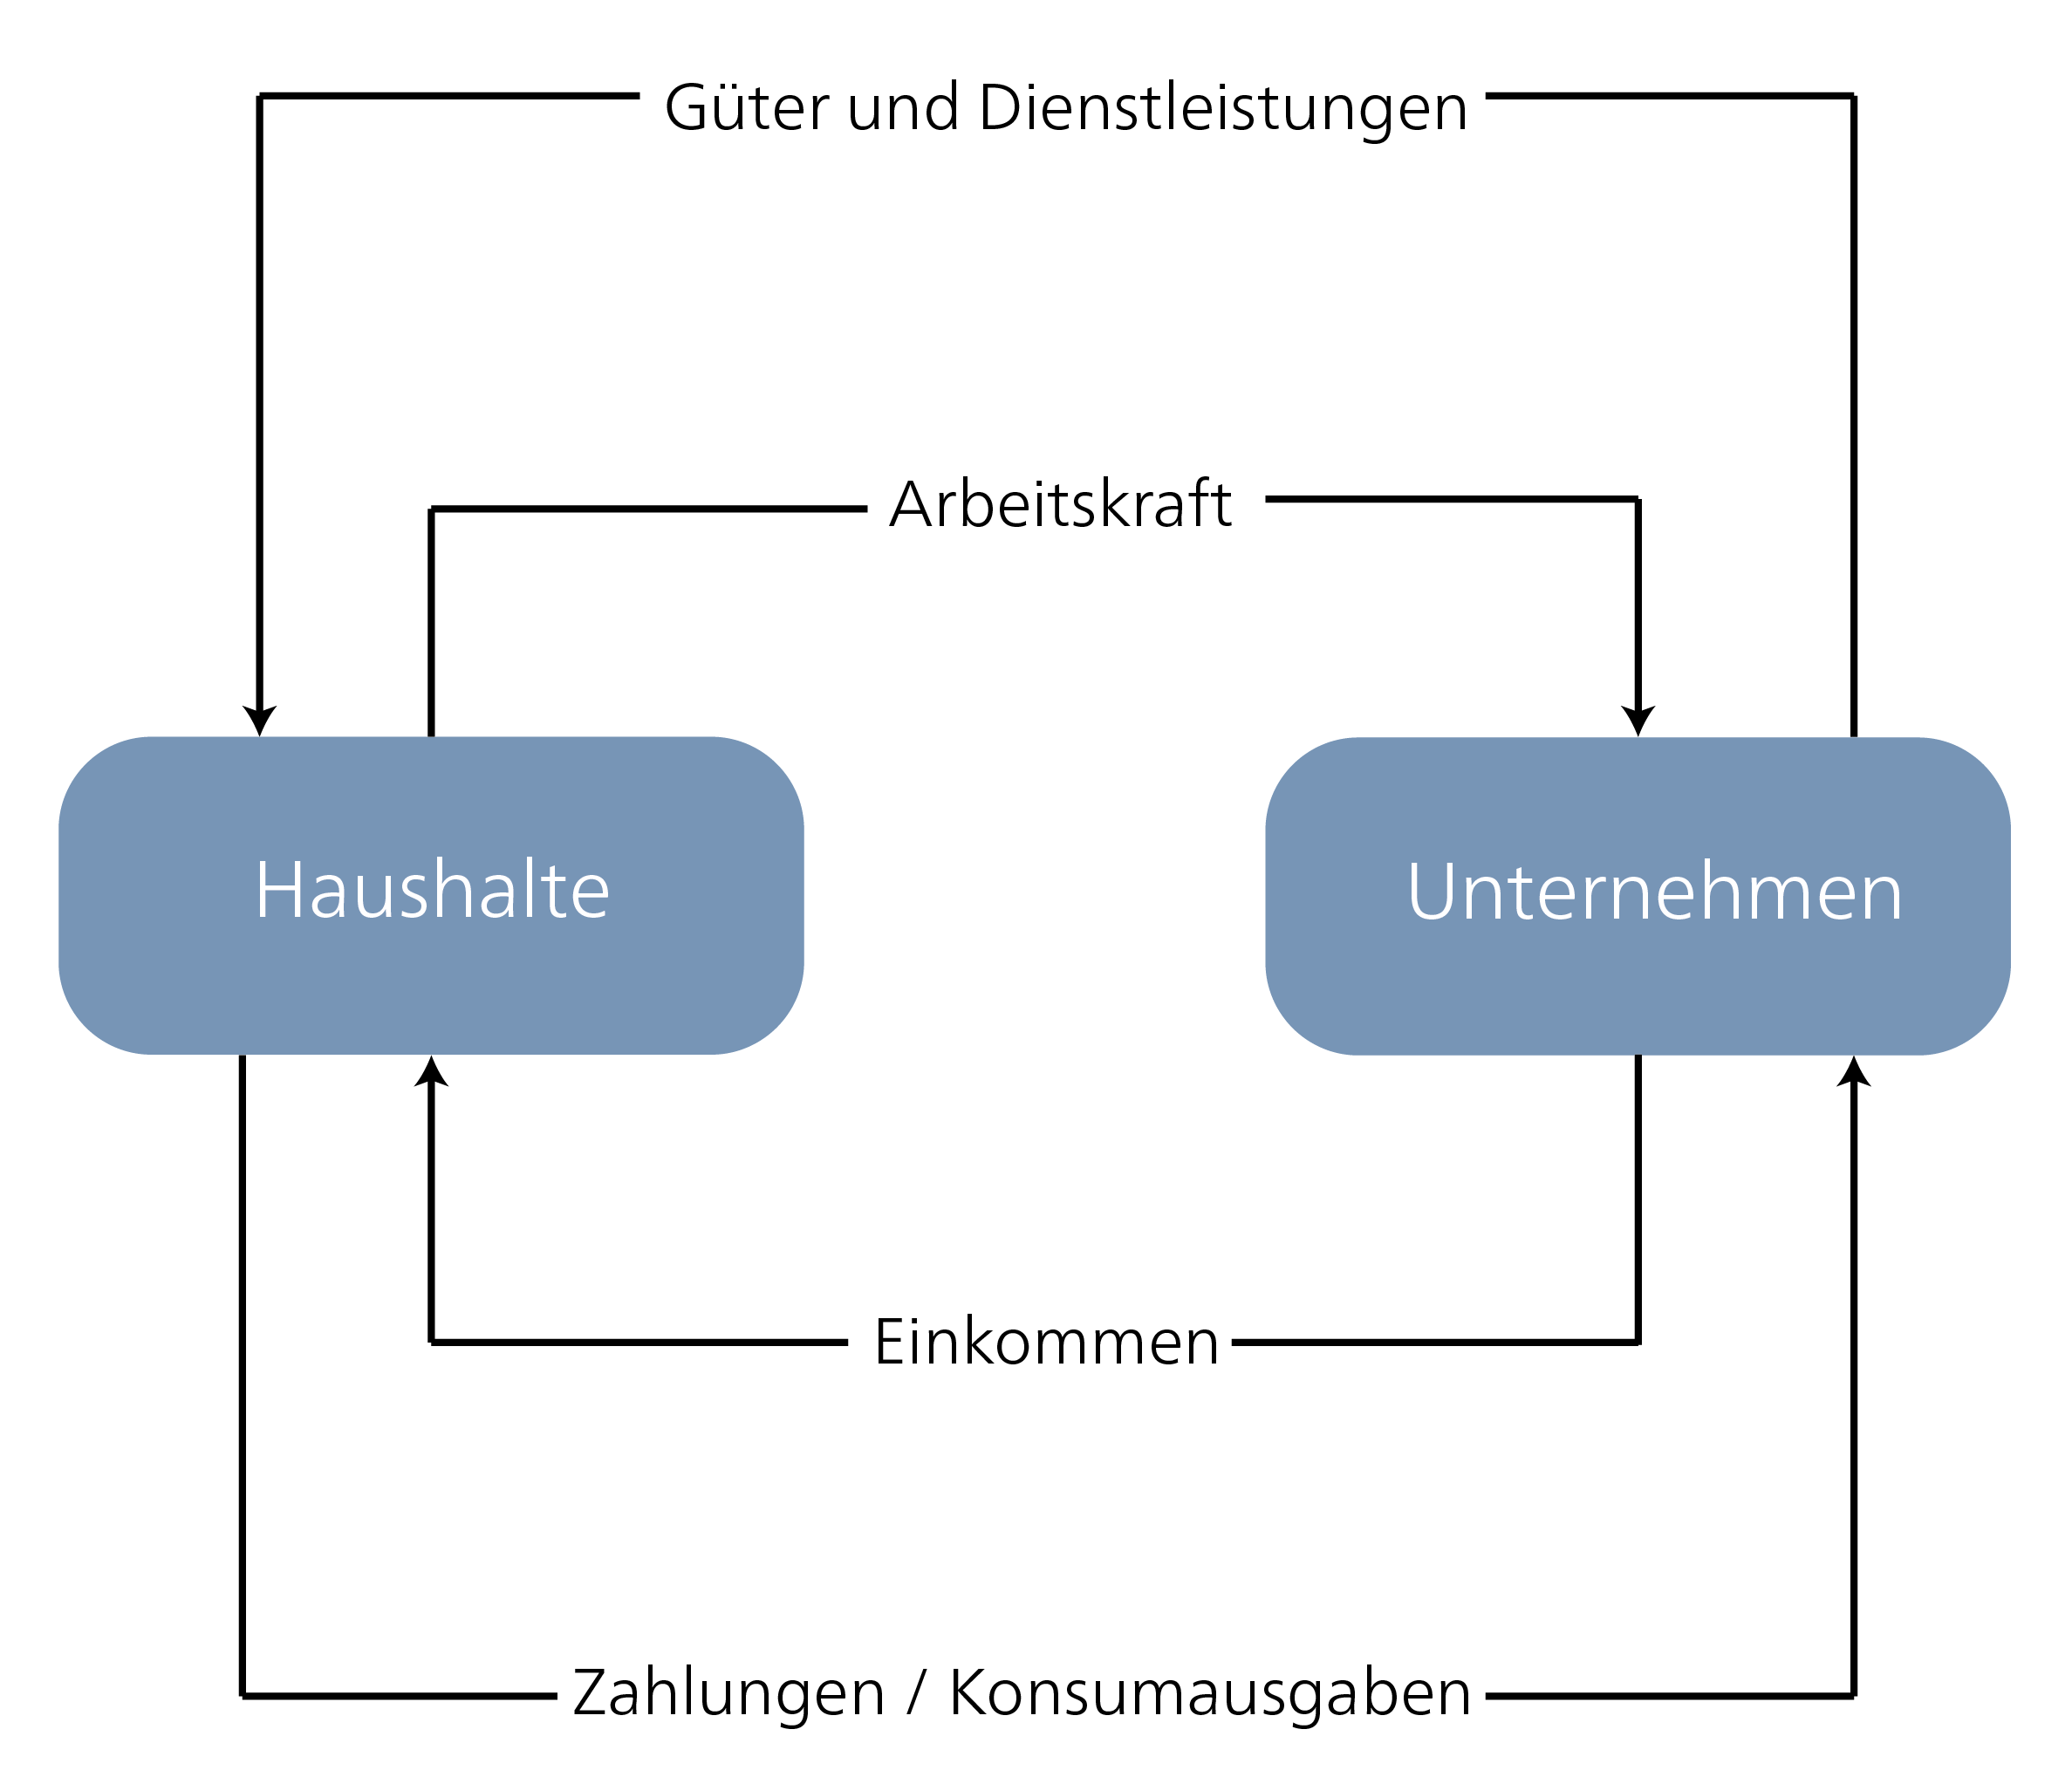
\includegraphics[keepaspectratio]{2_scope-of-economics/images/fig6.png}}

}

\caption{\label{fig-econ-cycle}\textbf{Simple economic circuit} -- Flows
of goods and money between households and firms: labour in exchange for
income, consumption expenditure in exchange for goods.}

\end{figure}%

\end{minipage}%
%
\begin{minipage}[t]{0.50\linewidth}

\begin{figure}[H]

\centering{

\pandocbounded{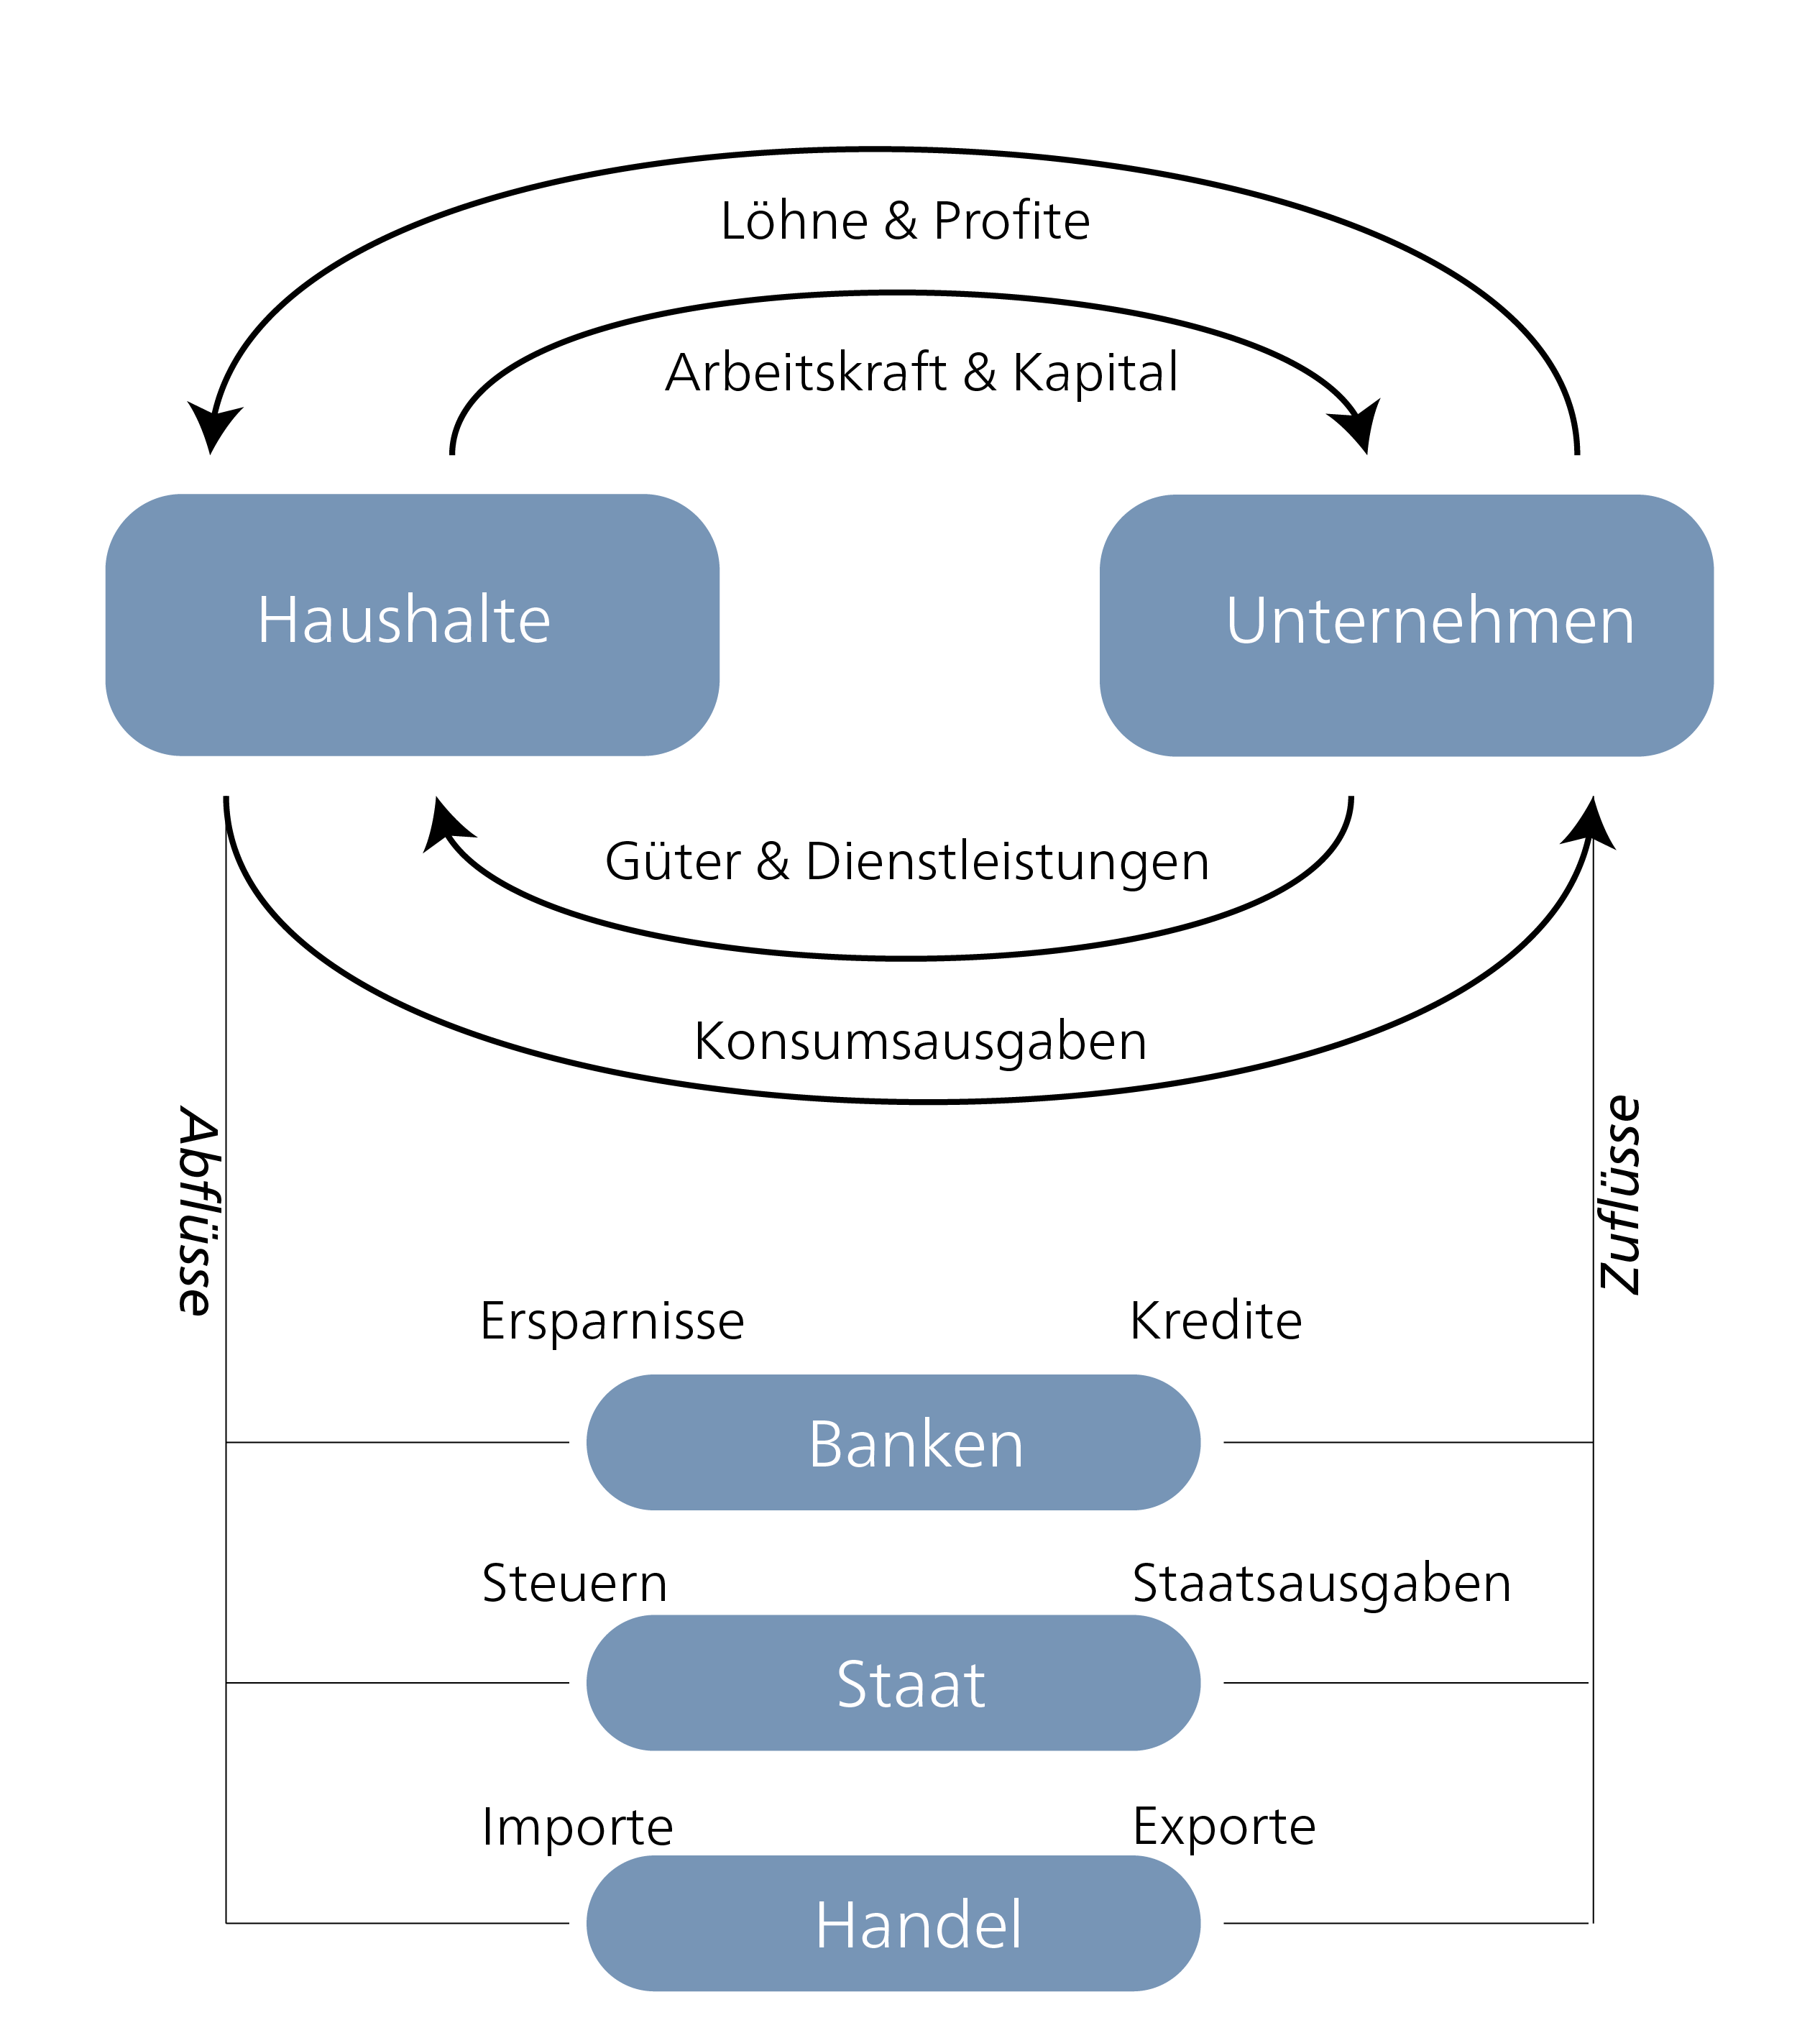
\includegraphics[keepaspectratio]{2_scope-of-economics/images/fig7.png}}

}

\caption{\label{fig-ext-cycle}\textbf{Extended economic circuit} --
Includes banks, the state, and foreign trade and shows how savings,
taxes, and imports act as \emph{outflows}, while credit, government
spending, and exports act as \emph{inflows}.}

\end{figure}%

\end{minipage}%
\newline
\begin{minipage}[t]{0.50\linewidth}
Source: Own illustrations after Rogall (2013) {[}p.~32{]} and Bäuerle et
al. (2026, 29).\end{minipage}%

\end{figure}%

Other schools of thought take other forms of provision into
consideration more explicitly. Feminist economics, for example,
emphasizes the importance of unpaid work as the basis of the paid
economy. Accordingly, it takes an important role in the depiction of
economic activities. For illustration,
Figure~\ref{fig-circular-flow-model} shows the circular flow model by
Diane Elson, which makes unpaid work visible. Ecological economics also
includes nature in such depictions, since nature too provides the basis
for all economic activity. In Chapter 3.1, we will look at this in more
detail.

\begin{figure}[H]

\centering{

\pandocbounded{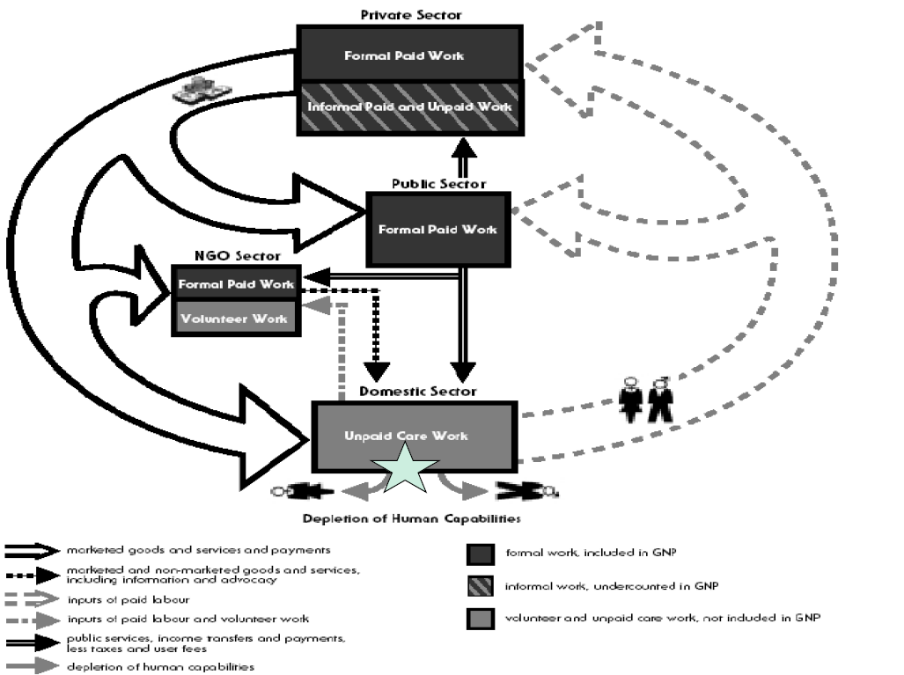
\includegraphics[keepaspectratio]{2_scope-of-economics/images/fig8.png}}

}

\caption{\label{fig-circular-flow-model}Circular flow model. Source:
Elson (2000).}

\end{figure}%

The schools of thought agree on the central importance of markets -- but
not on \emph{what} markets actually are and how they work. In what
follows, we compare two fundamentally different answers to our guiding
question: the abstract understanding of markets in neoclassical
economics and the political-economy understanding of capitalist markets.
A third perspective, institutional economics, which emphasizes the
active shaping of markets, will be taken up again later in the
discussion of the relationship between market and state (Chapter 5,
\emph{The Role of the State and Economic Policy Guiding Models}).

\subsection{How the market works in neoclassical
economics}\label{how-the-market-works-in-neoclassical-economics}

Neoclassical economics regards the \textbf{market as the central,
self-regulating institution} for providing goods and services. What is
central here is that markets are conceptualized abstractly, that is,
they are understood as independent of historical and societal
circumstances. This understanding implies that we are dealing here with
(quasi-)natural mechanisms or laws that apply universally. This is the
central difference from the political-economy perspective, which we
consider afterwards.

\subsection{The market as central coordinating
mechanism}\label{the-market-as-central-coordinating-mechanism}

In the neoclassical understanding, markets coordinate economic activity
through the interplay of supply (willingness to offer something) and
demand (willingness to acquire something). The profit and utility
functions of the actors, which can be calculated on the basis of the
marginal principle (see the excursus further below), form the basis for
supply and demand. Total demand results from the aggregation of the
individual functions. Firms try to maximize their profit, and
individuals try to maximize their utility (according to their
preferences) through consumption. In this starting position, competition
and the price mechanism subsequently determine how scarce resources are
distributed (as presented in Chapter x, this is the central economic
problem in neoclassical economics). If individuals can thus freely
decide what they want to buy and sell, the market mechanism ensures that
goods go where they create the highest utility, that is, to an efficient
or optimal market outcome. Market actors and structures are shaped
merely by these maximizations; there are no other influences, such as
the favouring or discrimination of persons or groups. No political or
moral goals are pursued.

In economics, markets are mostly represented by means of a
price-quantity diagram. The axes show quantity and price (or wage in
labour markets and interest rate in capital markets), and supply and
demand are depicted as curves. The slope of the curves changes with the
elasticity of supply and demand and shows how strongly these change when
quantity or price changes. Neoclassical economics assumes, on the one
hand, that the market tends towards an equilibrium and, on the other,
that this equilibrium represents the most efficient outcome. The
so-called Pareto efficiency (named after the economist Vilfredo Pareto)
serves as the central reference for assessing efficiency. A situation is
understood as Pareto-efficient, or Pareto-optimal, if no person can be
made better off (in terms of subjective utility) without something
having to be taken away from another person. As long as one person can
be made better off without our having to take something away from
another person, the situation counts as inefficient. As discussed in
Chapter 3.2, this also contains specific ideas of justice.

\begin{figure}[H]

{\centering \pandocbounded{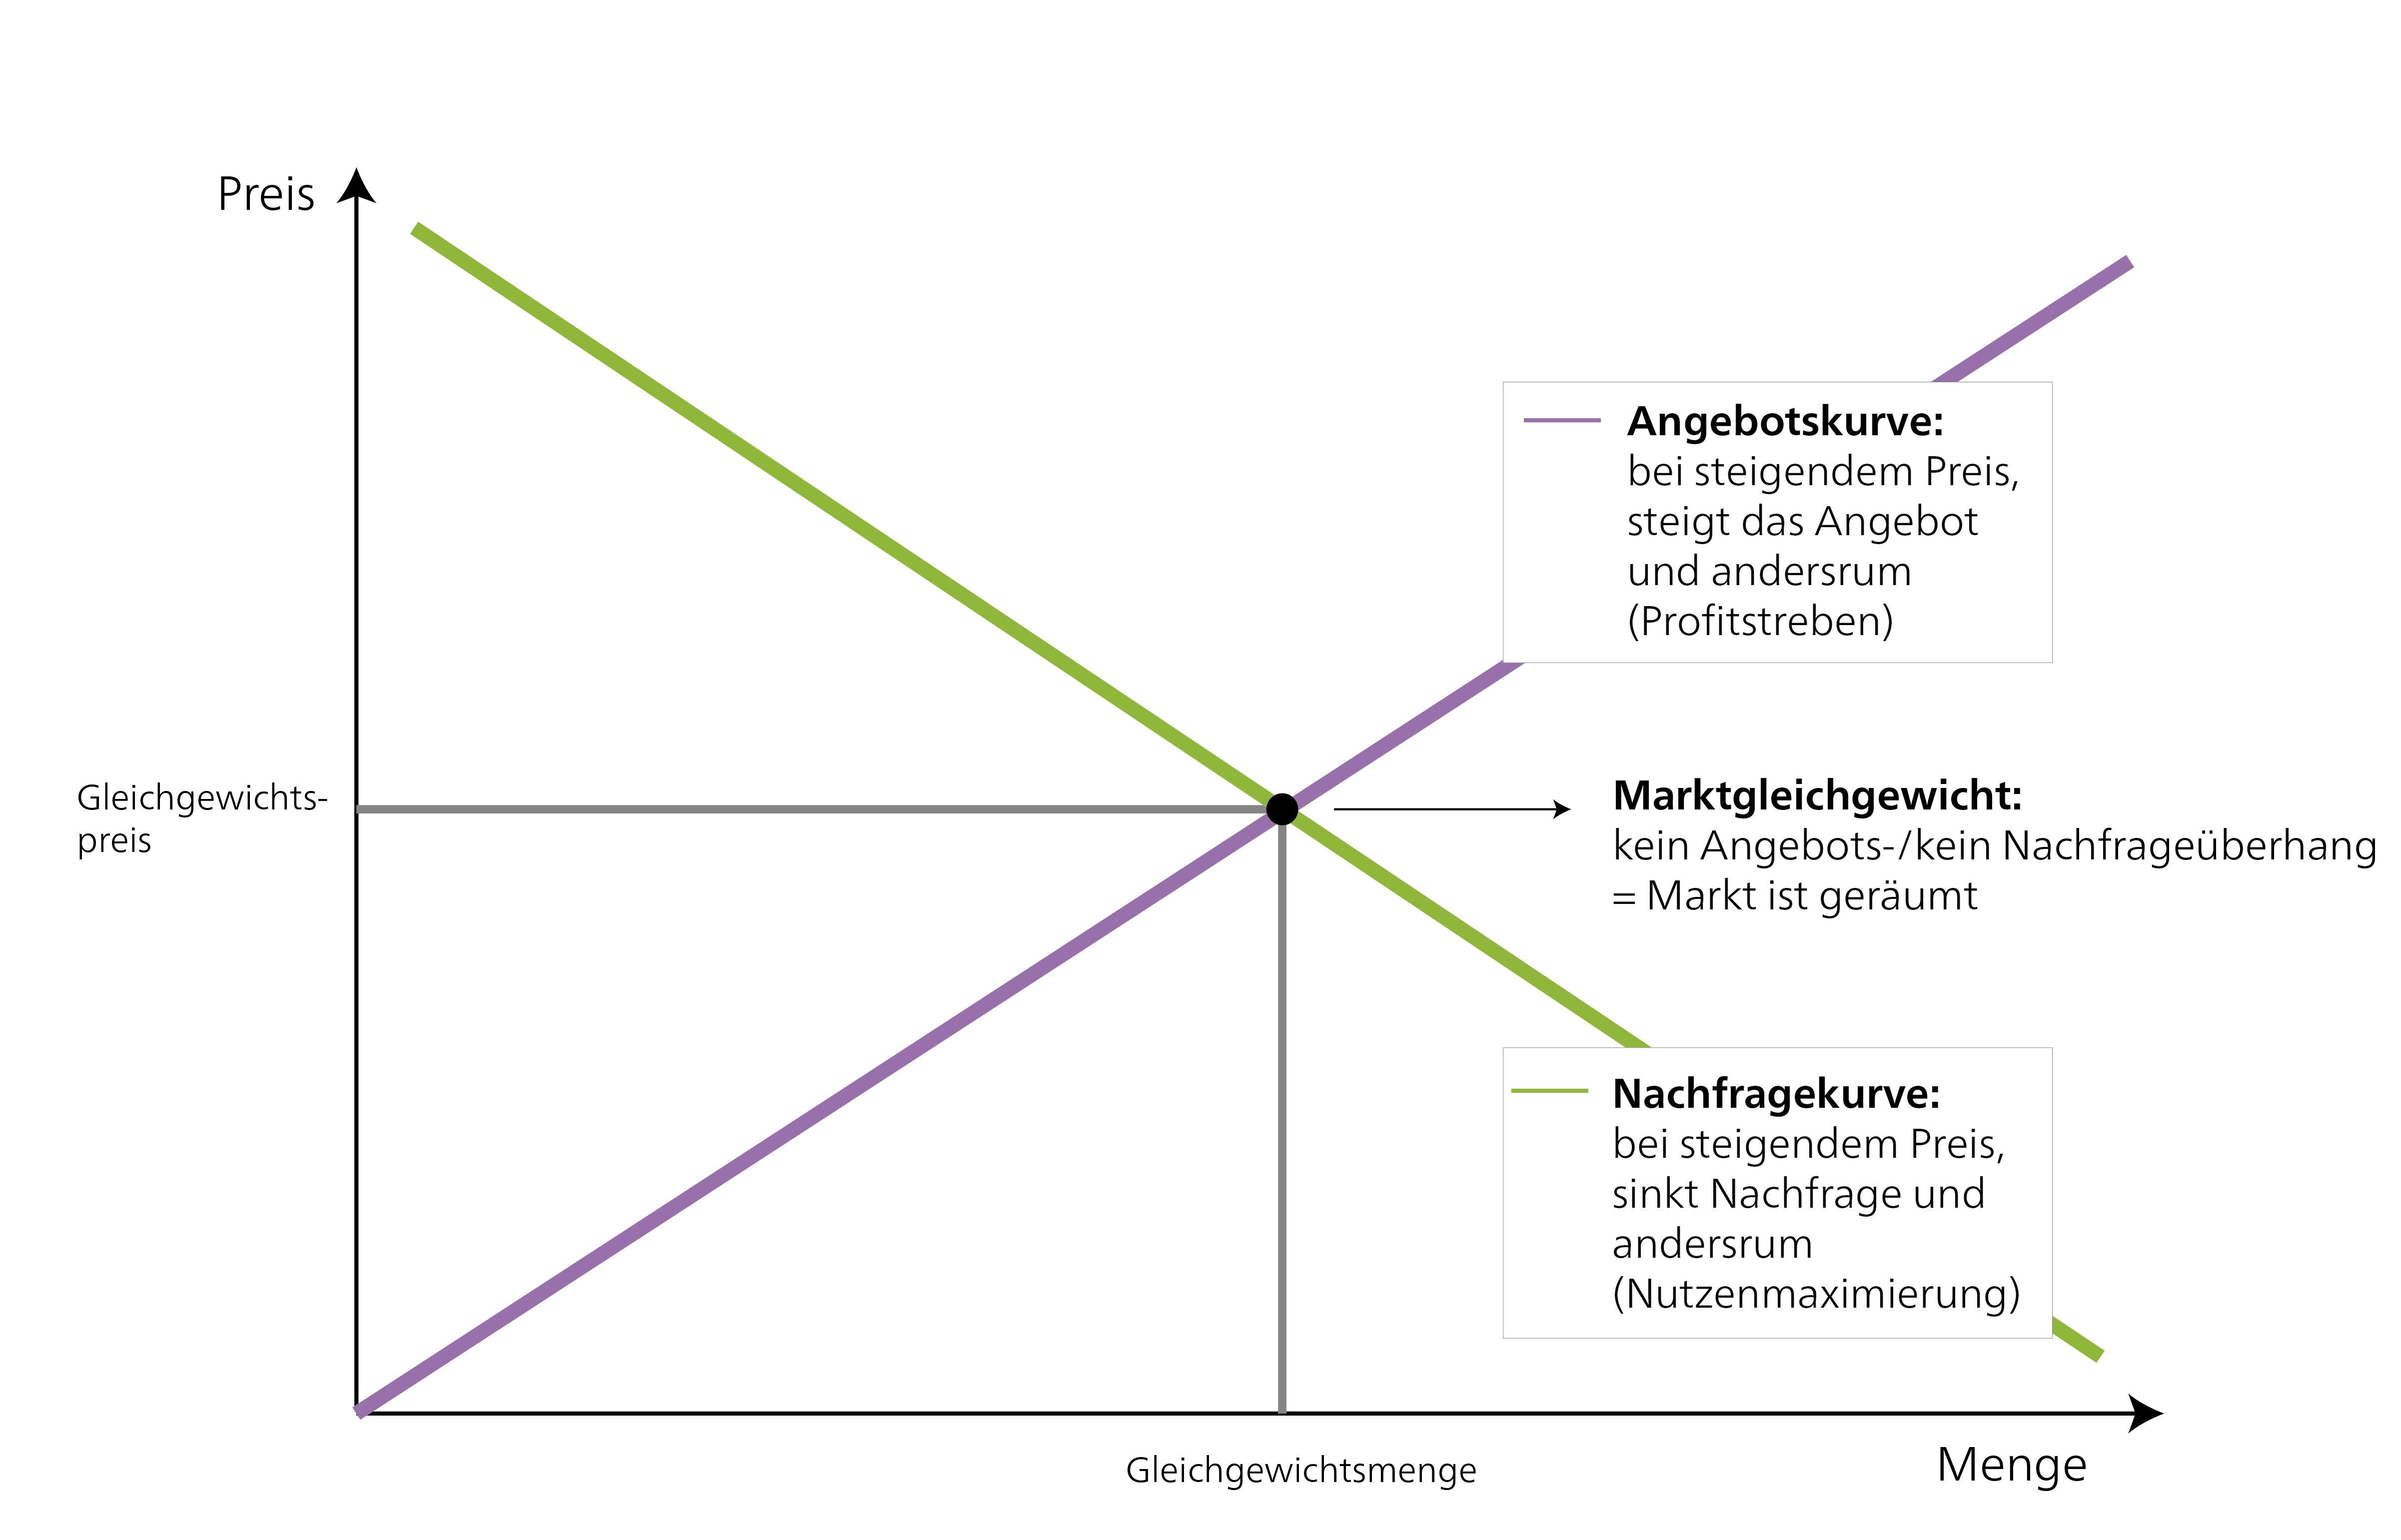
\includegraphics[keepaspectratio]{2_scope-of-economics/images/fig9.png}}

}

\caption{Graphical representation and determination of a market
equilibrium. Source: Own illustration.}

\end{figure}%

If the supply of a good is too high, the price falls -- if demand is too
high, it rises. In market equilibrium, demand equals supply and the
price stabilizes. In this way, the price mechanism decides who produces,
what and how much is produced, and for whom it is produced. The price is
therefore regarded as the central allocation instrument on markets. A
factory that produces with outdated machines, for example, cannot
produce at the same price as another factory with a more modern setup.
Because of its excessive production costs, it drops out of the market
and has to produce other goods or file for bankruptcy. Competition
ensures that this mechanism works and that inefficient firms exit the
market. A central assumption for the supply curve to slope upwards is
that, beyond a certain size, the marginal costs of firms rise again
(even in the long run), for example through increased coordination
effort, so that there is, to a certain extent, a limit to growth for
firms. This assumption is contested, however (see, for example, Keen
2010; Pirgmaier 2017). If this assumption is not met, the supply curve
could also have a different slope, and there would be no guaranteed
market equilibrium with many competitive firms; there could also be a
tendency towards monopoly. Even Alfred Marshall, the founder of this
price-quantity diagram, repeatedly wrestled with the question of whether
there might not also be a tendency towards monopoly (Marshall 1919, 316;
2013, 324).

The central basic assumption for this way markets work is that of
perfect competition. Under \textbf{perfect competition}, individual
suppliers have no influence on the price, since if the price rises,
buyers purchase from other suppliers. Firms have to take the market
price as a given quantity and can decide only on the quantity they
offer. They are accordingly in the role of price takers and quantity
adjusters.

For perfect competition to be possible, several preconditions are
necessary:

\begin{itemize}
\tightlist
\item
  There is a large number of suppliers and buyers in the market. This
  state is called a \textbf{polypoly}. If there are only a few suppliers
  or buyers, one speaks of an oligopoly or oligopsony, respectively. If
  there is even only one supplier or buyer, one speaks of a monopoly or
  monopsony, respectively (for an overview, see
  Table~\ref{tbl-market-forms}).
\item
  All actors have \textbf{complete information}, that is, there are no
  hidden agreements among certain market participants or firms that
  offer inferior goods without disclosing it.
\item
  Consumers have \textbf{no preferences at all for individual
  suppliers}. Markets work fully only if consumers can choose between
  the different suppliers without obstacles. Otherwise, a supplier could
  raise the price above the market price and still have customers.
\end{itemize}

If the above preconditions are not met, market failure can occur, and
the market no longer works optimally. In a neoclassical understanding,
when market failure arises, the state should intervene with regulations.
As long as no market failure occurs, however, the state should keep out
as far as possible and only guarantee the framework conditions. In
Chapter 5, we then look more closely at how the relationship between the
market and the state can be understood.

\begin{table}

\caption{\label{tbl-market-forms}Market forms matrix: market forms by
number of suppliers and buyers. The polypoly is a condition for the
assumption of perfect competition. Source: Own illustration after
\href{https://studyflix.de/wirtschaft/marktformen-1492}{studyflix}.}

\centering{

\centering
\begin{tabular}[t]{>{\raggedright\arraybackslash}p{3cm}>{\raggedright\arraybackslash}p{3.8cm}>{\raggedright\arraybackslash}p{3.8cm}>{\raggedright\arraybackslash}p{3.8cm}}
\toprule
\multicolumn{1}{c}{ } & \multicolumn{3}{c}{Buyers} \\
\cmidrule(l{3pt}r{3pt}){2-4}
\textbf{Suppliers} & \textbf{one buyer} & \textbf{few buyers} & \textbf{many buyers}\\
\midrule
\textbf{one supplier} & Bilateral monopoly & Limited monopoly & Monopoly\\
\textbf{few suppliers} & Limited monopsony & Bilateral oligopoly & Oligopoly\\
\textbf{many suppliers} & Monopsony & Oligopsony & Polypoly\\
\bottomrule
\end{tabular}

}

\end{table}%

\subsubsection{Types of markets}\label{types-of-markets}

\begin{figure}[H]

{\centering \pandocbounded{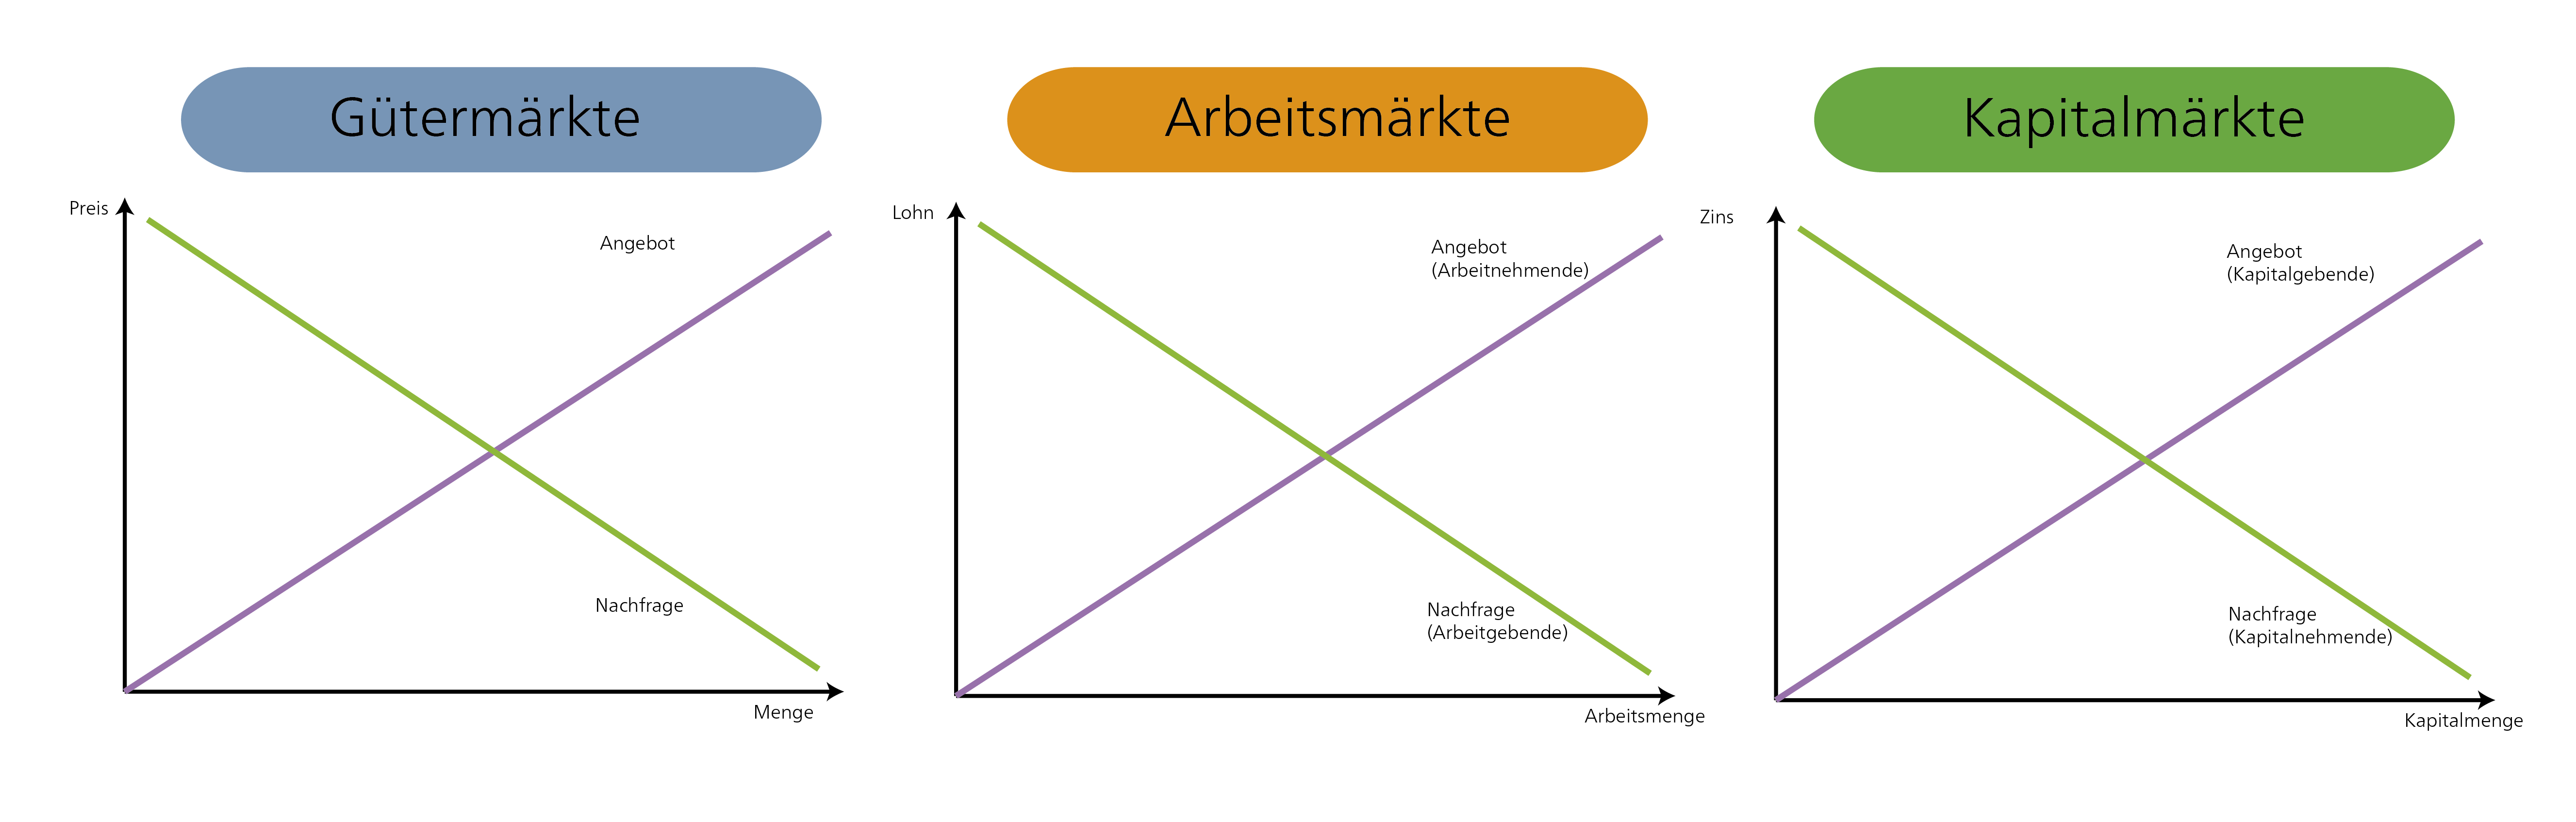
\includegraphics[keepaspectratio]{2_scope-of-economics/images/fig11.png}}

}

\caption{Different types of markets. Source: Own illustration.}

\end{figure}%

This market mechanism of coordinating supply and demand is applied to
various markets. A key distinction is made between goods markets and
factor markets. On \textbf{goods markets}, goods and services are
traded. On \textbf{factor markets}, the factors of production (land,
capital, labour) are offered and demanded. Households, for example,
offer their labour power on the labour market, and instead of a price,
the level of the wage paid arises through the price mechanism from the
demand of firms. In the neoclassical understanding, all these markets
fundamentally work according to the same logic. The labour market works
on the same principle as the market for potatoes. Other schools of
thought, for example post-Keynesian economics, emphasize that labour
markets differ strongly from goods markets.

\begin{tcolorbox}[enhanced jigsaw, arc=.35mm, bottomrule=.15mm, bottomtitle=1mm, breakable, colback=white, colbacktitle=quarto-callout-note-color!10!white, colframe=quarto-callout-note-color-frame, coltitle=black, left=2mm, leftrule=.75mm, opacityback=0, opacitybacktitle=0.6, rightrule=.15mm, title={In-depth questions}, titlerule=0mm, toprule=.15mm, toptitle=1mm]

\begin{itemize}
\tightlist
\item
  For each of the three preconditions of perfect competition, think of
  examples from today's economy where they are met and where they are
  not.
\item
  Are there differences in the demand for different goods? What
  influence does this have on markets for food, cars, and leisure
  activities?
\item
  Think about the advantages and disadvantages of conceptualizing the
  market as an abstract concept, that is, independently of the
  historically specific context.
\end{itemize}

\end{tcolorbox}

\begin{tcolorbox}[enhanced jigsaw, arc=.35mm, bottomrule=.15mm, bottomtitle=1mm, breakable, colback=white, colbacktitle=quarto-callout-tip-color!10!white, colframe=quarto-callout-tip-color-frame, coltitle=black, left=2mm, leftrule=.75mm, opacityback=0, opacitybacktitle=0.6, rightrule=.15mm, title={Excursus: Price level}, titlerule=0mm, toprule=.15mm, toptitle=1mm]

Given the great importance of the price mechanism for the functioning of
markets, the price level in an economy is one of the most important
variables that is observed and analysed. Price-level stability is
measured by the inflation rate of goods and services. With low inflation
of up to 2\%, one speaks of a stable price level. Statistical offices
use a standardized ``basket of goods'' to record how the price index of
the cost of living changes over time. The composition of the basket
differs between countries and mostly covers only goods markets, not
capital markets.

In Switzerland, the Federal Statistical Office (FSO) compiles the
\href{https://www.bfs.admin.ch/bfs/de/home/statistiken/preise/erhebungen/lik/warenkorb.html}{Swiss
Consumer Price Index (CPI)}. The figure below shows which consumer goods
make up this index and in what proportions. The basket contains ``the
most important goods and services consumed by private households''
{[}our translation{]}. The weighting is based on annual household
surveys and is meant to reflect their actual consumption behaviour as
accurately as possible.

\begin{figure}[H]

{\centering \pandocbounded{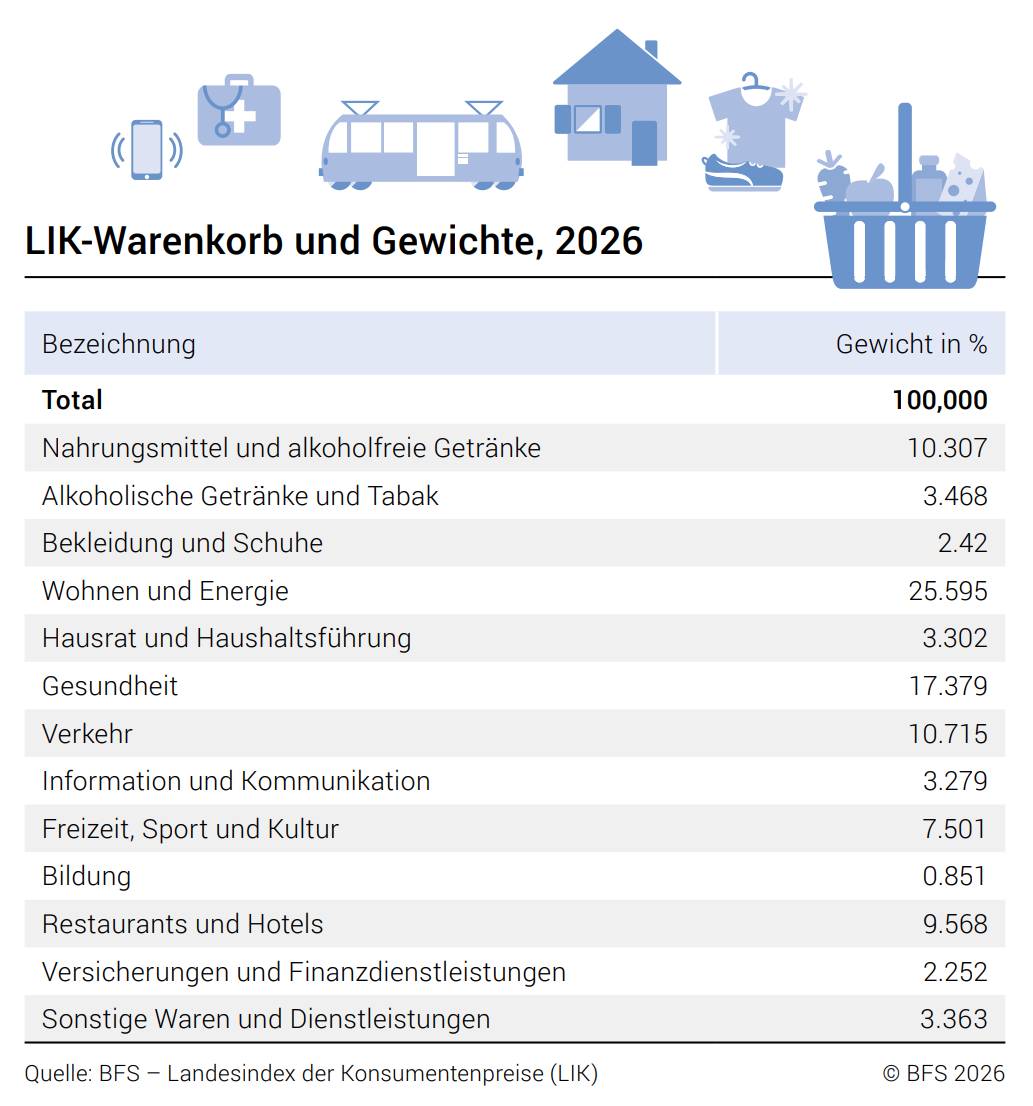
\includegraphics[keepaspectratio]{2_scope-of-economics/images/fig12.png}}

}

\caption{Composition of the basket of goods for the Swiss Consumer Price
Index 2026. Source: BFS (2026).}

\end{figure}%

\end{tcolorbox}

\begin{tcolorbox}[enhanced jigsaw, arc=.35mm, bottomrule=.15mm, bottomtitle=1mm, breakable, colback=white, colbacktitle=quarto-callout-tip-color!10!white, colframe=quarto-callout-tip-color-frame, coltitle=black, left=2mm, leftrule=.75mm, opacityback=0, opacitybacktitle=0.6, rightrule=.15mm, title={Excursus: The invisible hand of the market}, titlerule=0mm, toprule=.15mm, toptitle=1mm]

The term invisible hand is often used to describe the
\textbf{self-regulation of markets}. The term goes back to Adam Smith.
Adam Smith used the term twice in his earlier work \emph{The Theory of
Moral Sentiments} (1759) and once in his work \emph{The Wealth of
Nations} (1776). In \emph{The Wealth of Nations}, Smith uses the term in
the chapter on ``restraints upon the importation from foreign countries
of such goods as can be produced at home''. In this context, Smith
writes that if someone prefers to support domestic rather than foreign
industry, this person is led by an invisible hand. Noam Chomsky
therefore interprets Smith as describing a ``home bias'' in this
passage. Different economists have interpreted the passage in different
ways, however. The most popular interpretation sees in this passage the
justification of the self-regulating forces of the market. Market
activity, it holds, is a regulating force that leads individuals to
satisfy their individual needs as well as possible, which at the same
time serves society by distributing goods as well as possible. Such an
interpretation is contested in view of the surrounding context and is
repeatedly criticized by experts in the history of theory.

\begin{quote}
``He generally, indeed, neither intends to promote the public interest,
nor knows how much he is promoting it. By preferring the support of
domestic to that of foreign industry, he intends only his own security;
and by directing that industry in such a manner as its produce may be of
the greatest value, he intends only his own gain, and he is in this, as
in many other cases, led by an invisible hand to promote an end which
was no part of his intention.'' (Smith and Recktenwald 2013, 371)
\end{quote}

\end{tcolorbox}

\begin{tcolorbox}[enhanced jigsaw, arc=.35mm, bottomrule=.15mm, bottomtitle=1mm, breakable, colback=white, colbacktitle=quarto-callout-tip-color!10!white, colframe=quarto-callout-tip-color-frame, coltitle=black, left=2mm, leftrule=.75mm, opacityback=0, opacitybacktitle=0.6, rightrule=.15mm, title={Excursus: The marginal principle -- marginal utility and marginal cost}, titlerule=0mm, toprule=.15mm, toptitle=1mm]

The marginal principle is central to the conceptualization of the market
from a neoclassical perspective, since it takes on the explanation of
the emergence of value and utility and thus of demand. The marginal
principle has its origins around 1870 in the marginalist revolution and
to this day forms the basis of neoclassical economics. It deals with the
question of the value of commodities, which also influences the
allocation of goods, services, and factors of production. In contrast to
classical economics, the marginal principle of neoclassical economics
detaches itself from the objective theory of value and formulates the
subjective theory of value.

The objective theory of value of classical economics postulates that all
commodities have an objective value. The labour put into the production
of the commodity was commonly used as the basis for determining this
value, which founded the labour theory of value. In the subjective
theory of value, by contrast, no absolute values are considered but the
subjective values that people attribute to commodities and their
marginal changes relative to the starting position. This focus on
marginal changes founds the marginal principle. The marginal principle
made it possible to transfer differential calculus to cost, utility, and
yield functions, as a result of which the use of mathematical models in
economics experienced a lasting boom.

\textbf{Yield function of land and marginal yield}

The marginal principle was originally observed in the yield function of
land. Studies of agriculture in the 18th century revealed the
relationship between factor input and yield. The marginal yield is the
increase in yield through one additional unit of a factor of production.

\begin{quote}
``It lies in the nature of agriculture -- and this is a very noteworthy
circumstance -- that the additional product does not rise in direct
proportion to the number of additional workers employed; rather, each
worker employed later delivers a smaller product than the one before.''
Johann Heinrich von Thünen 1850, secondary quotation after Winfried
Reiss in \emph{Mikroökonomische Theorie: Historisch fundierte
Einführung} (2007, pp.~90f.) {[}our translation{]}.
\end{quote}

What von Thünen observed with the factor labour, A. R. J. Turgot also
found with the use of the factor capital in the form of fertilizer. The
principle of marginal yield can equally be transferred to industrial
production and, for example, to the number of workers in a factory.

\textbf{Gossen's laws}

In 1854, Hermann Heinrich Gossen developed his laws of human intercourse
and the rules for human action flowing from them. In them, he formulated
the lawfulness of individual preferences and their satisfaction, which
is oriented towards the respective utility.

\textbf{Gossen's first law: The law of diminishing marginal utility}

The law of diminishing marginal utility, also called the law of
satiation, reads:

\begin{quote}
``The magnitude of one and the same pleasure decreases continuously if
we continue to prepare that pleasure without interruption, until satiety
finally occurs.'' Hermann Heinrich Gossen in \emph{Entwicklung der
Gesetze des menschlichen Verkehrs, und der daraus fliessenden Regeln für
menschliches Handeln} (1854, p.~4) {[}our translation{]}.
\end{quote}

The utility of the first cup of coffee in the morning is greater than
that of the third or fourth. It is similar with living space, where, for
example, the first bathroom in a flat is of greater use to the residents
than the second. According to the theory, this law can in principle be
transferred to all goods.

\textbf{Gossen's second law: The law of equalization of marginal
utilities}

The law of equalization of marginal utilities, also called the law of
equalization of pleasures, states:

\begin{quote}
``A human being who is free to choose between several pleasures but
whose time is not sufficient to prepare all of them fully must, however
different the absolute magnitude of the individual pleasures may be, in
order to bring the sum of his pleasure to the greatest, before he fully
prepares even the greatest one, prepare them all partially, and in such
a proportion that the magnitude of each pleasure, at the moment when its
preparation is broken off, remains the same for all'' Hermann Heinrich
Gossen in \emph{Entwicklung der Gesetze des menschlichen Verkehrs, und
der daraus fliessenden Regeln für menschliches Handeln} (1854, p.~12)
{[}our translation{]}.
\end{quote}

This law aims at the optimal use of limited means for different goods.
An individual's optimal utility is reached when the marginal utility
(that is, the utility of the next additional unit) is the same for all
goods. Mathematically, this means that the marginal utility functions of
the different goods are set equal. The marginal utility corresponds to
the maximum price that the person concerned is willing to pay. From the
aggregation of the marginal utility (functions) of all individuals, the
total demand (function) can be determined. The marginal principle
accordingly forms the core of neoclassical consumer theory. For
interested students (who are familiar with the basics of neoclassical
economics), the \href{https://ilias.unibe.ch/go/file/3803482}{critical
discussion of neoclassical consumer theory by Ben Fine} (in German) is
recommended.

\textbf{Marginal cost and marginal yield in firms}

As derived above, marginal yield describes the yield of an additional
unit. Analogously, the term \textbf{marginal cost} describes the cost of
an additional unit. Marginal costs can be determined by differentiating
the mathematical cost function. The costs {[}C{]} of a firm result from
the sum of the fixed costs {[}C\textsubscript{f}{]} (for example rent,
machines) and the variable costs {[}C\textsubscript{v}{]} (labour power,
raw materials, intermediate products).

\[C = C_f + C_v\]

According to neoclassical theory, firms orient themselves, besides the
cost function, on the revenue function. This describes how much revenue
{[}R{]} arises from the sale of a good depending on quantity {[}X{]} and
price {[}P{]}.

\[R = P * X\]

Differentiating the revenue function yields marginal revenue, the
revenue of one additional unit sold. A firm produces until marginal cost
exceeds marginal revenue. This can be calculated by setting the
differentiated cost and revenue functions equal. In market equilibrium
(under perfect competition), the price theoretically equals marginal
cost. Although neoclassical theory focuses strongly on price, it has
engaged little with how firms set prices. In his dissertation,
Nubbemeyer (2010) shows that until the middle of the 20th century it was
controversially discussed whether firms actually orient themselves
towards the marginal principle or towards alternative concepts (for
example mark-up pricing, as in some post-Keynesian models) when setting
prices. Although the debate has not been conclusively resolved, the idea
of the marginal principle dominates economics.

\end{tcolorbox}

\subsection{Markets as arenas of power and distribution -- capitalist
production
system}\label{markets-as-arenas-of-power-and-distribution-capitalist-production-system}

While neoclassical economics regards markets as universal institutions,
other schools of thought examine capitalist markets in their historical
and societal specificity. That is, these analyses do not claim universal
validity but want to understand the dynamics on capitalist markets in a
specific context.

From this perspective, markets are not a natural state but are actively
\textbf{shaped and regulated} by actors, institutions, property rights,
and laws. This immediately raises our guiding question: Who determines
the ``rules of the game'', and whose interests do they serve? This
question opens up the view to \textbf{power and distribution}, which
play a central role in political-economy perspectives. A
political-economy perspective means that economic, political, and
societal aspects and structures are understood in relation to one
another, so that power, institutions, and distribution, for example,
receive central attention. Political economy is thus a collective term,
and different schools of thought can take a political-economy
perspective (there is also a strand of political economy in neoclassical
economics). Marxist and post-Keynesian economics, as well as parts of
feminist and ecological economics, understand themselves in principle as
political-economic. In contrast to neoclassical economics, capitalist
markets in this perspective are moreover regarded as inherently
\textbf{unstable}. Class conflicts and power dynamics are thus not an
exception but structurally built in.

To make this perspective more concrete, we ask in the next section: What
exactly makes an economic system \emph{capitalist}?

\subsection{What actually makes an economic system
capitalist?}\label{what-actually-makes-an-economic-system-capitalist}

There are many different definitions of what constitutes the essence of
a capitalist economic system. Some central aspects can nevertheless be
identified (Fraser 2022):

\begin{itemize}
\item
  The means of production are predominantly in private ownership.
\item
  The majority of employees are separated from the means of production.
  They thus do not own the means of production. They therefore have to
  sell their labour power for a wage.
\item
  Economic decisions and the distribution of goods are predominantly
  coordinated through markets.
\item
  Firms produce predominantly with the aim of making profits.
  Competitive pressure means that a large part of these profits is
  reinvested, so that constant capital accumulation becomes a central
  feature of the capitalist economy. This leads to a compulsion for
  constant growth.
\end{itemize}

These conditions may seem very ordinary to us. Many of us do wage work,
we encounter markets everywhere, and competition and the profit motive
seem so self-evident in economic policy news that they need no further
explanation. In fact, however, this way of doing business became
dominant only in the course of the 19th century with the rise of
industrialization in England. Before that, in Western Europe, peasants
were bound to the land and the landlord through the feudal system, and
the economy was largely shaped by agriculture. Production for one's own
needs and local supply dominated in many places. In addition, the
communal use of land and resources, alongside seigneurial and private
ownership, played an important role in supplying the population. Markets
(for example weekly markets, annual fairs, and so on) also played a role
but were of less importance in everyday life and for supplying the
population than they are today. Moreover, markets were strongly embedded
in society and in a moral system -- ideas of a just price, for example,
played a central role.

An influential, predominantly Marxist interpretation sees a decisive
step in the emergence of capitalism in the fact that people were
separated from their access to land and the means of production. Over
centuries, more and more land in common ownership, that is, commons, was
privatized. Through these enclosures and the privatization of communally
used land, many peasant households lost their livelihood and
increasingly became dependent on wage labour (Polanyi 2017). This was in
part a very violent process and illustrates that markets do not arise
independently of societal and political processes. They are actively
created and shaped by various actors, state interventions, property
rights, laws, and so on. It becomes clear that power is also a central
factor.

But how and when exactly capitalism emerged is still contested in
scholarship today. While some authors see its origin above all in
changed class relations and conflicts in England (for example Wood
2015), others emphasize the central role of colonialism, slavery, and
global trade (for example Beckert and Dierlamm 2026). Many current works
try to combine these two perspectives. And while some locate the origin
of capitalism as early as the Middle Ages, others see the decisive steps
of its emergence only in the industrial capitalism of the 19th century.
Here too, it is a question of perspective and of the understanding of
what exactly capitalism is (for example, whether we can already locate
capitalist elements in long-distance trade from the 16th century onwards
or not).

\subsubsection{Why do companies (and entire economies) actually have to
grow
constantly?}\label{why-do-companies-and-entire-economies-actually-have-to-grow-constantly}

A central dynamic of the capitalist economy is the accumulation of
capital. Firms do not produce only to provide goods but to make profits
and to invest these profits again in the production process. Marx
describes this dynamic as a movement from money (M) through the
production of commodities (C) back to more money (M') -- (often
summarized in this notation: M-C-M'): capital is used to produce
commodities whose sale generates a larger sum of money. Capital must
thus multiply continuously. This dynamic is not determined solely by the
individual profit interests of individual firms but also arises from
competitive pressure between firms. Firms that do not invest, bring
forth innovations, or raise their productivity risk losing market share.
Competition thereby creates systemic pressure towards growth, expansion,
and constant productivity increases. Several tensions arise from this
growth dynamic:

\begin{itemize}
\item
  \textbf{Capital vs.~labour:} Since the majority of people do not own
  means of production, they depend on selling their labour power for a
  wage. At the same time, firms strive to make profits by raising labour
  productivity and reducing costs. Profits and wages thus stand in an
  inverse relationship, since higher wages usually mean lower profits
  and vice versa. Marx describes this relationship as the fundamental
  class conflict between capital and labour. In doing so, Marx describes
  a process of exploitation. Firms do not pay employees the full value
  they create through their work and skim off the rest as profit (this
  remainder is also called surplus value). Since workers do not receive
  the full value of their work, Marx calls this process exploitation. In
  Marxist theory, exploitation describes not primarily a moral judgement
  of individual firms but a social relation (see also Chapter 2.3.2,
  \emph{Capital -- why do some people own capital and others do not?}).
\item
  \textbf{Distribution of income and demand:} While firms may have an
  interest in reducing wage costs, wages are at the same time the most
  important source of income for a large part of the population and thus
  a central basis for consumer demand. Strong pressure on wages can
  therefore raise the profitability of individual firms in the short
  term but contribute to weaker aggregate demand in the long term.
  Marxist approaches describe this as a possible tendency towards crises
  of overproduction: firms can produce more than can be sold given the
  available purchasing power. Post-Keynesian approaches also take up
  this problem but emphasize in particular the importance of demand for
  economic development. If demand falls (rises), firms tend to invest
  less (more), which in turn can have a negative (positive) effect on
  economic development.
\item
  \textbf{Competition and concentration:} On the one hand, competition
  is regarded as an important mechanism for innovation and efficiency
  gains. On the other hand, competition can lead in the long term to a
  concentration of capital, since successful firms can gain market share
  and displace smaller firms. As a result, dominant firms and
  monopoly-like structures can emerge.
\item
  \textbf{Societal and ecological limits:} Feminist economists point out
  that the capitalist economy depends on labour that often takes place
  outside markets, in particular unpaid care and reproductive work.
  These activities create the preconditions for the paid economy to be
  possible at all. Ecological economists also emphasize that capitalist
  accumulation is based on the use of natural resources. The continuous
  expansion of production and consumption can thereby come into conflict
  with the limited ecological capacities of the planet.
\end{itemize}

The growth dynamic described and its tensions mean that capitalist
economic systems are particularly dependent on growth. Matthias
Binswanger (2019) even argues that capitalist economic systems are
subject to a \textbf{growth imperative}. Firms must make profits to
finance investments and to survive in the long term. If firms on average
do not earn profits, this can lead to a downward spiral: investment
declines, employment falls, and aggregate demand decreases. Growth thus
stabilizes not only individual firms but the entire economic system.
Schmelzer and Vetter (2019) argue in turn that \textbf{growth
dependency} does not necessarily mean that every single economic
activity must grow. Rather, a longer-term absence of growth can create
considerable economic and societal tensions. A phase of stagnation or
shrinkage can lead to rising unemployment, falling incomes, corporate
crises, and a burden on public budgets (Schmelzer and Vetter 2019). If
growth fails to materialize, the system thus falls into crisis.

This compulsion or dependency is reinforced by institutional factors.
Modern, credit-based financial systems, for example, presuppose future
growth so that loans can be repaid. In addition, in many countries --
including Switzerland -- social insurance systems are closely tied to
paid employment. High employment and rising incomes thereby become
important preconditions of societal stability. Growth is thus not only
an economic goal but deeply embedded in societal institutions. According
to Hartmut Rosa (2003), growth has even become a central cultural
expectation.

From the perspective of ecological economics, this orientation towards
growth is fundamentally problematic, since economic growth has
historically been, and continues to be, closely coupled with rising
energy and resource consumption. Whether growth can be permanently
decoupled from environmental pressure is the central point of contention
between green growth and post-growth approaches -- more on this in
self-study phase 6.

\subsection{Are financial crises accidents -- or built into the
system?}\label{are-financial-crises-accidents-or-built-into-the-system}

Money and credit are an important precondition for capitalist dynamics.
Through loans, firms can make investments, expand production capacities,
and finance innovations. Since the 1980s, there has been increasing
liberalization and deregulation of financial markets in many countries.
In the period after the Great Depression of 1929, banks and financial
markets were still strongly regulated. With the deregulation of the
1980s, the role of the financial sector within capitalist economic
systems also changed. While financial markets originally had above all
the task of enabling productive investment, financial returns and
short-term increases in value gained increasing importance. This
development is called \emph{financialization}. It refers to the growing
importance of financial markets, financial institutions, and financial
motives for firms, households, and states. Firms, for example, orient
themselves more strongly towards short-term return targets and
increasing share value, while financial institutions increasingly make
profits by trading financial assets such as shares, bonds, commodities,
or derivatives. With the importance of the financial market for the
economy as a whole, the power of the financial industry also grows.

Deregulation relied above all on theories from neoclassical economics,
which argued that deregulated financial markets would function
efficiently in principle because of their information processing and the
rationality of individual market participants (Fama 1970). The great
financial crisis of 2008 fundamentally called these assumptions into
question, however. While the financial crisis represents, from a
neoclassical perspective, an exogenous shock, that is, an external shock
that disturbed the equilibrium, other schools of thought, above all
post-Keynesian economics, emphasize that financial crises arise from the
system itself and that the system is thus inherently unstable.
Post-Keynesian economics emphasizes that investment depends primarily on
expectations about future profits. Firms invest when they expect future
revenue to exceed the cost of the investment. These expectations are
fundamentally uncertain, however. As a result, investment and economic
activity can be subject to strong fluctuations. With his financial
instability hypothesis, Hyman Minsky (1992) shows that phases of
economic stability in particular can generate new instabilities. In
times of rising confidence, firms and households increasingly take on
credit, and financial institutions are willing to take on higher risks.
A dynamic can thereby develop in which rising asset prices and
increasing indebtedness initially reinforce economic expansion. At the
same time, however, the system becomes more prone to crises. If
expectations are disappointed, lending, investment, and consumption can
fall abruptly. The great financial crisis of 2008 was an impressive
example of this. From this perspective, financial crises are therefore
not simply external disturbances of an otherwise stable market system
but can arise from the normal dynamics of capitalist financial systems.

The tensions described, as well as the instability of the financial
system, do not mean that capitalist societies inevitably collapse. But
they show that capitalist markets do not find a stable equilibrium on
their own. Instead, they are unstable and prone to crises. Historically,
capitalist societies have developed various mechanisms to limit these
conflicts and to establish stability. These include, for example, state
regulation, social insurance, labour rights, public investment, or the
opening up of new markets. The concrete shape of capitalism therefore
differs strongly between historical periods and also between different
regions. An often-discussed example of stabilization is the Fordist
accumulation regime after the Second World War, when employees largely
accepted the capitalist order of ownership and economy and firms
accepted rising wages and the expansion of the welfare state.
Productivity growth then translated strongly into rising wages. This was
a development that, however, stalled from the 1970s onwards. This then
had strong effects on the lives of many people. In Chapter 3, we discuss
the social limits and will also go into these developments in depth.

\begin{tcolorbox}[enhanced jigsaw, arc=.35mm, bottomrule=.15mm, bottomtitle=1mm, breakable, colback=white, colbacktitle=quarto-callout-note-color!10!white, colframe=quarto-callout-note-color-frame, coltitle=black, left=2mm, leftrule=.75mm, opacityback=0, opacitybacktitle=0.6, rightrule=.15mm, title={In-depth questions}, titlerule=0mm, toprule=.15mm, toptitle=1mm]

\begin{itemize}
\tightlist
\item
  Think about where in your everyday life you encounter tensions of the
  capitalist mode of production and how they affect your everyday life.
\item
  Look for examples of interactions between the economy, politics, and
  society.
\item
  Are you aware of current processes of enclosure? How are they
  connected to the capitalist mode of production?
\end{itemize}

\end{tcolorbox}

\begin{tcolorbox}[enhanced jigsaw, arc=.35mm, bottomrule=.15mm, bottomtitle=1mm, breakable, colback=white, colbacktitle=quarto-callout-caution-color!10!white, colframe=quarto-callout-caution-color-frame, coltitle=black, left=2mm, leftrule=.75mm, opacityback=0, opacitybacktitle=0.6, rightrule=.15mm, title={Further material -- Oeconomia: Economic growth, debt, inequality, and
profits}, titlerule=0mm, toprule=.15mm, toptitle=1mm]

In 2020, Carmen Losmann made a
\href{https://www.3sat.de/film/dokumentarfilm/oeconomia-100.html}{documentary
film} (in German) on the relationship between economic growth, debt,
inequality, and profits. The film deals with these complex relationships
in a very accessible way and stimulates reflection. Even though the film
is in part somewhat imprecise, it is well worth watching as an
introduction.

\end{tcolorbox}

\chapter{Problem Analysis: What Ails Our
Economy?}\label{problem-analysis-what-ails-our-economy}

\begin{tcolorbox}[enhanced jigsaw, arc=.35mm, bottomrule=.15mm, bottomtitle=1mm, breakable, colback=white, colbacktitle=quarto-callout-note-color!10!white, colframe=quarto-callout-note-color-frame, coltitle=black, left=2mm, leftrule=.75mm, opacityback=0, opacitybacktitle=0.6, rightrule=.15mm, title={Guiding question}, titlerule=0mm, toprule=.15mm, toptitle=1mm]

If prosperity for all -- within ecological limits -- is the goal we took
as our starting point in Chapter 2: Why do we not achieve this goal, and
what exactly stands in its way?

\end{tcolorbox}

The current way of doing business leads to major challenges, which
manifest themselves in various crises. The current crises are referred
to as a multiple crisis and, more recently, increasingly as a
\textbf{polycrisis} (see, for example, Lawrence et al. 2024 or this
\href{https://www.weforum.org/videos/experts-explain-adam-tooze-what-is-the-polycrisis/}{explainer
video} by Adam Tooze), because they touch people's working and living
worlds in many ways and are interwoven with one another. Some of the
individual crises are strongly connected and share common causes. Others
appear rather independent of one another and do not necessarily have the
same causes. Taken as a whole, however, all these crises culminate in
this polycrisis, which often seems overwhelming. In this chapter, we
devote ourselves to the \textbf{analysis of these crises} before turning
to solutions for a sustainable economy. In what follows, we address the
ecological and social problems separately. It is important to stress,
however, that these dimensions are closely linked and can reinforce one
another. The separation of these areas is meant to make the introduction
easier.

As became apparent in the preceding chapters, the analysis itself is
also shaped by the perspective a person takes. The problem analysis
would turn out differently depending on the school of thought.
Neoclassical economics, for example, does not necessarily see rising
income and wealth inequality as a problem as long as it comes about
through market mechanisms. A school of thought that includes aspects of
power in its analysis, such as the feminist or the Marxist one, sees
this inequality as a central problem for the economy and society. In
line with the orientation of the course, we will frame the problem
analysis as broadly as possible, across as many schools of thought as
possible. Later in the course, we will also see more precisely which
analyses and conclusions come from which school of thought. In the
self-study phase, we first address the ecological limits of current
economic activity and the relationship between nature and the economy.
Then, in the fourth self-study phase, we look at the social limits of
the current system and at how the economy and society are related.

\section{Ecological Limits -- How Much Earth Do We Actually Have -- and
How Much Do We
Use?}\label{ecological-limits-how-much-earth-do-we-actually-have-and-how-much-do-we-use}

The ecological limits of our economic activity have been concretely
tangible for some time and are not just abstract discussions about
climate models. We can feel them in our everyday lives. While this
script was being written in the summer of 2026, the fourth heatwave
arrived in Switzerland, wildfires raged in France and Spain, and the
consequences of heat and drought were noticeable everywhere in Europe.
In the context of a sustainable economy, the question arises of how we
connect these developments with economic activities or, more generally,
how we can understand the relationship between the economy and nature.
How we understand this relationship influences what we perceive as a
problem and also forms the basis of the range of possibilities within
which we can think about and develop solutions. Here, we will focus
mainly on neoclassical and ecological economics, since they have two
fundamentally different understandings of this relationship. While
ecological economics emphasizes that the economy is embedded in the
natural environment and necessarily depends on nature as its foundation,
neoclassical economics understands nature and the economy as two
separable spheres. Before we go into the basic understandings of this
relationship in more detail (3.1.2) and look at what they mean for the
problem analysis, we briefly look at some basic aspects of the
ecological crises.

\subsection{Planetary boundaries and climate
crisis}\label{planetary-boundaries-and-climate-crisis}

\begin{figure}[H]

\centering{

\pandocbounded{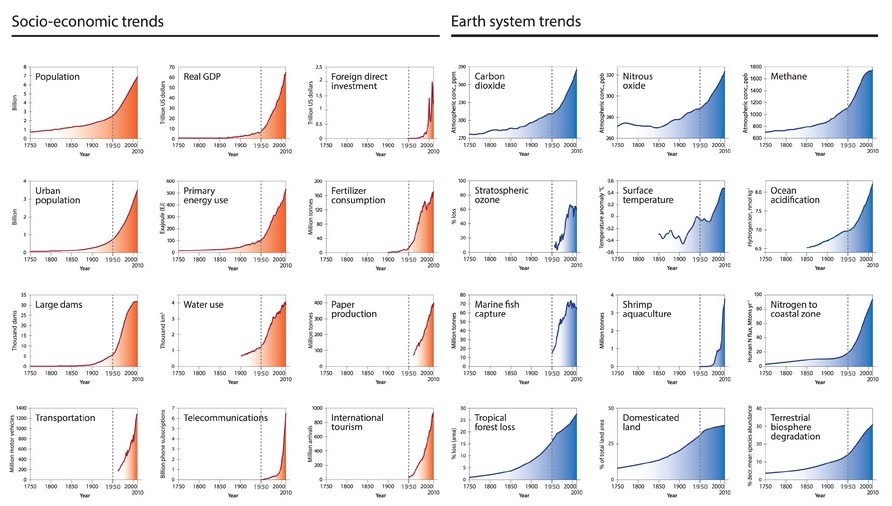
\includegraphics[keepaspectratio]{3_problem-analysis/images/fig1.png}}

}

\caption{\label{fig-acceleration}Trends of various socioeconomic and
Earth system indicators between 1750 and 2010. The rapid increase is
called the ``Great Acceleration'', and its effects are regarded as an
indicator of the new Anthropocene epoch. Source:
https://futureearth.org/the-great-acceleration/.}

\end{figure}%

In the wake of the Industrial Revolution, a uniquely productive mode of
production emerged, which enabled a massive increase in material
prosperity. At the same time, but far less noted, there was also a
massive increase in the consumption of natural resources, environmental
pollution, and emissions (Jarrige et al. 2020). Socioeconomic growth
went hand in hand with the acceleration of biophysical trends. The
description of exponential growth dynamics is called ``the Great
Acceleration'' (Steffen et al. 2015). The graphic above shows, by way of
example, some important biophysical and socioeconomic indicators, all of
which begin to rise with the Industrial Revolution. From the middle of
the 20th century, the tendency towards exponential growth becomes
obvious.

\begin{tcolorbox}[enhanced jigsaw, arc=.35mm, bottomrule=.15mm, bottomtitle=1mm, breakable, colback=white, colbacktitle=quarto-callout-tip-color!10!white, colframe=quarto-callout-tip-color-frame, coltitle=black, left=2mm, leftrule=.75mm, opacityback=0, opacitybacktitle=0.6, rightrule=.15mm, title={Excursus: Exponential growth}, titlerule=0mm, toprule=.15mm, toptitle=1mm]

The exponential function is used to describe the size of things that are
subject to accelerating growth. A decisive step is the realization that
even moderate growth of, for example, five per cent means exponential
growth, so the increase keeps getting larger (this applies, for example,
to economic growth or to case numbers during the COVID-19 pandemic).
Exponential growth is hard for us humans to grasp and is commonly
underestimated, since the slope is quite moderate at the beginning. The
growth rate, however, keeps increasing, because the moderate increase in
the following year refers to the value that rose in the previous year --
and at some point it becomes enormous. A revealing figure that quickly
exposes growth processes is the doubling time, which can easily be
calculated in one's head: 70 divided by the percentage growth per unit
of time. If something grows by seven per cent per year, the doubling
time is ten years; at five per cent, it is fourteen years; and at one
per cent growth, it is seventy years. The number 70 is the result of
multiplying 100 (the percentage value of a doubling) by the natural
logarithm of 2. You do not need to understand how this number is
derived. All that matters is: 70 divided by the percentage growth.

For those who are interested, there is a documentary on exponential
growth:
``\href{https://www.3sat.de/wissen/wissenschaftsdoku/211216-sendung-wido-100.html}{Understanding
exponential growth: The water lily principle}'' (in German). The
following \textbf{thought experiment} also helps with understanding: A
client offers you two different fees for a 64-day assignment. Which fee
do you choose? A: You receive CHF 10,000 every day. B: You receive CHF
0.01 on the first day, and on every following day the amount is doubled.

Table~\ref{tbl-payoff-matrix} shows the payoff matrix for this thought
experiment.

\begingroup\fontsize{8}{10}\selectfont

\begin{longtable}[t]{lll}

\caption{\label{tbl-payoff-matrix}Thought experiment: Payoff matrix
under linear versus exponential growth.}

\tabularnewline

\toprule
\textbf{Number of days} & \textbf{Payout A} & \textbf{Payout B}\\
\midrule
\endfirsthead
\multicolumn{3}{@{}l}{\textit{(continued)}}\\
\toprule
\textbf{Number of days} & \textbf{Payout A} & \textbf{Payout B}\\
\midrule
\endhead

\endfoot
\bottomrule
\endlastfoot
8 days & CHF 80,000 & CHF 1.28\\
21 days & CHF 210,000 & CHF 10,485\\
26 days & CHF 260,000 & CHF 335,544\\
30 days & CHF 300,000 & CHF 5,368,709\\
64 days & CHF 640,000 & CHF 92,233,720,368,547,758\\*

\end{longtable}

\endgroup{}

The payout of B after 64 days is more than 92 quadrillion CHF, which
corresponds to about 95,000 times the wealth of Elon Musk (according to
\href{https://www.forbes.at/artikel/elon-musk-verliert-den-billionaersstatus}{Forbes},
the richest person on Earth as of June 2026).

\end{tcolorbox}

Since the late 18th century, when the Briton Thomas Robert Malthus
(1766-1834) first put forward a theory of overpopulation in his
\emph{Essay on the Principle of Population}, the discourse of a
planetary carrying capacity has persisted in certain scientific
theories. Even though Malthus's ideas have meanwhile turned out to be
outdated -- he calculated the maximum population depending on a fixed
quantity of producible food -- the basic idea returns in the form of
neo-Malthusianism. In the study \emph{The Limits to Growth}, published
by the Club of Rome in 1972, a neo-Malthusian approach calculated a
population limit also by means of available food, but additionally
including available resources, environmental pollution, and industrial
output. Although the predicted developments did not materialize, the
study still carries weight today in an ecological perspective that
problematizes limitless growth.

The latest theoretical development in this regard is the natural-science
concept of \textbf{planetary boundaries}. Unlike before, these do not
refer to a maximum population but to indicators from Earth system
science. As a starting point, the researchers choose the state of the
Earth system in the Holocene (the current and latest epoch of Earth's
history, which began about 11,700 years ago). In this epoch, they argue,
the planet had largely ideal conditions for giving rise to human
civilizations. Deviations from this bring humanity into an uncertain
zone in which tipping points can be reached. Crossing them can either
halt previous developments, change their direction, or accelerate them
strongly. One example is the extinction of many large mammals at the end
of the last ice age following human migration to the American continent.
The concept of planetary boundaries advises applying the precautionary
principle here in order to reduce possible harm to humans and the
environment. The current Planetary Health Check takes the planetary
boundaries as a fundamental framework for evaluating the health of our
planet (Ceasar et al. 2024; Sakschewski et al. 2025). The recently
founded initiative
``\href{https://www.planetaryhealthcheck.org/}{Planetary Health Check}''
offers, besides the report, exciting opportunities on its website to
engage with the planetary boundaries and their development over the last
70 years.

\begin{figure}[H]

{\centering \pandocbounded{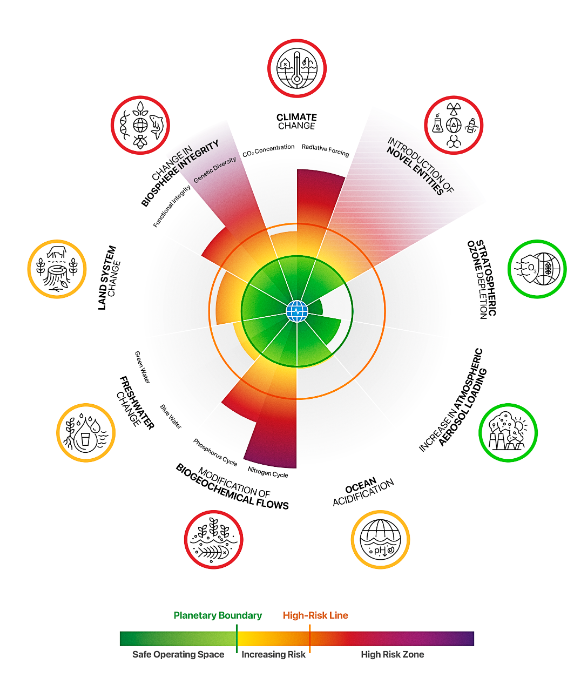
\includegraphics[keepaspectratio]{3_problem-analysis/images/fig2.png}}

}

\caption{Planetary boundaries of the various subsystems and the
respective risk assessment of the current state. Green denotes the safe
operating space, yellow an increased uncertainty. Beyond yellow
indicates that the risk of fatal consequences is assessed as high.
Source: Sakschewski et al. (2025, 29).}

\end{figure}%

The planetary boundaries refer to nine different subsystems, such as
land-use change or ocean acidification. For each of them, an inner
circle (safe operating space) and an outer circle (increased
uncertainty) are defined. Seven of the nine planetary boundaries have
already been crossed (Sakschewski et al. 2025). For ocean acidification,
the boundary has recently been crossed for the first time, while aerosol
loading is declining somewhat again. While the trend for stratospheric
ozone levels does not show a clear direction, the degree of
transgression is increasing for all boundaries previously identified as
crossed (Sakschewski et al. 2025).

Within these nine subsystems, there are two so-called core boundaries:
biosphere integrity and climate change. These two systems combine the
processes of many other subsystems and act at a supraregional level.
Reaching tipping points in these two systems can therefore push the
entire Earth system into a new state. The rapid changes in the climate
in particular pose a major challenge to humanity in the 21st century.
Because the energy system, the transport infrastructure, and industrial
agriculture are based on fossil fuels such as oil and gas, excessive
amounts of greenhouse gases such as carbon dioxide and nitrogen oxides
are continually emitted. These accumulate in the atmosphere and prevent
the heat that reaches the atmosphere through solar radiation from
escaping again (greenhouse effect). As a result, glaciers and ice sheets
have shrunk, the oceans have become warmer, and sea levels have risen
over the last 30 years. Extreme temperature anomalies and precipitation
events are also continually increasing. Today, the concentration of
greenhouse gases in the Earth's atmosphere is the highest in the last
800,000 years, and the global average temperature has risen by more than
one degree Celsius since the Industrial Revolution.

To avoid reaching tipping points in the climate, climate policy set the
two-degree target with the Paris Agreement in 2015. The rise in average
temperature since the Industrial Revolution is to be kept ``well below 2
degrees Celsius''. Even at two degrees of warming, massive biophysical
changes are likely. And to reach this target, energy supply must forgo
fossil fuels entirely from 2050. Such a shift poses major challenges for
society, in particular because fossil energies were a central factor in
the development of the current economic system and strongly structure it
(see, for example, Huber 2013; Kallis and Sager 2017; Malm 2016).

\subsection{Different understandings of the nature-economy
relationship}\label{different-understandings-of-the-nature-economy-relationship}

\emph{↗ Textbook chapter 7}

As already discussed in Chapter 2 on the scope of economics, some
schools of thought understand the economy mainly as a separate sphere in
which actors interact on markets. Others emphasize the embeddedness of
economic activities in society and nature. We already encountered this
distinction in Chapter 2.3.1, where we dealt with land as a factor of
production. Neoclassical economics focuses very strongly in its
understanding on a separate economic sphere. These efforts to study a
separate economic sphere in isolation go back, among other things, to
the marginalist revolution, when attempts were made, among other things,
to separate economic motives from non-economic motives in humans.
Accordingly, in this understanding, the economy stands to some extent
alongside nature, and the two are of equal standing (see
Figure~\ref{fig-econ-nature}).

\begin{figure}[H]

\centering{

\pandocbounded{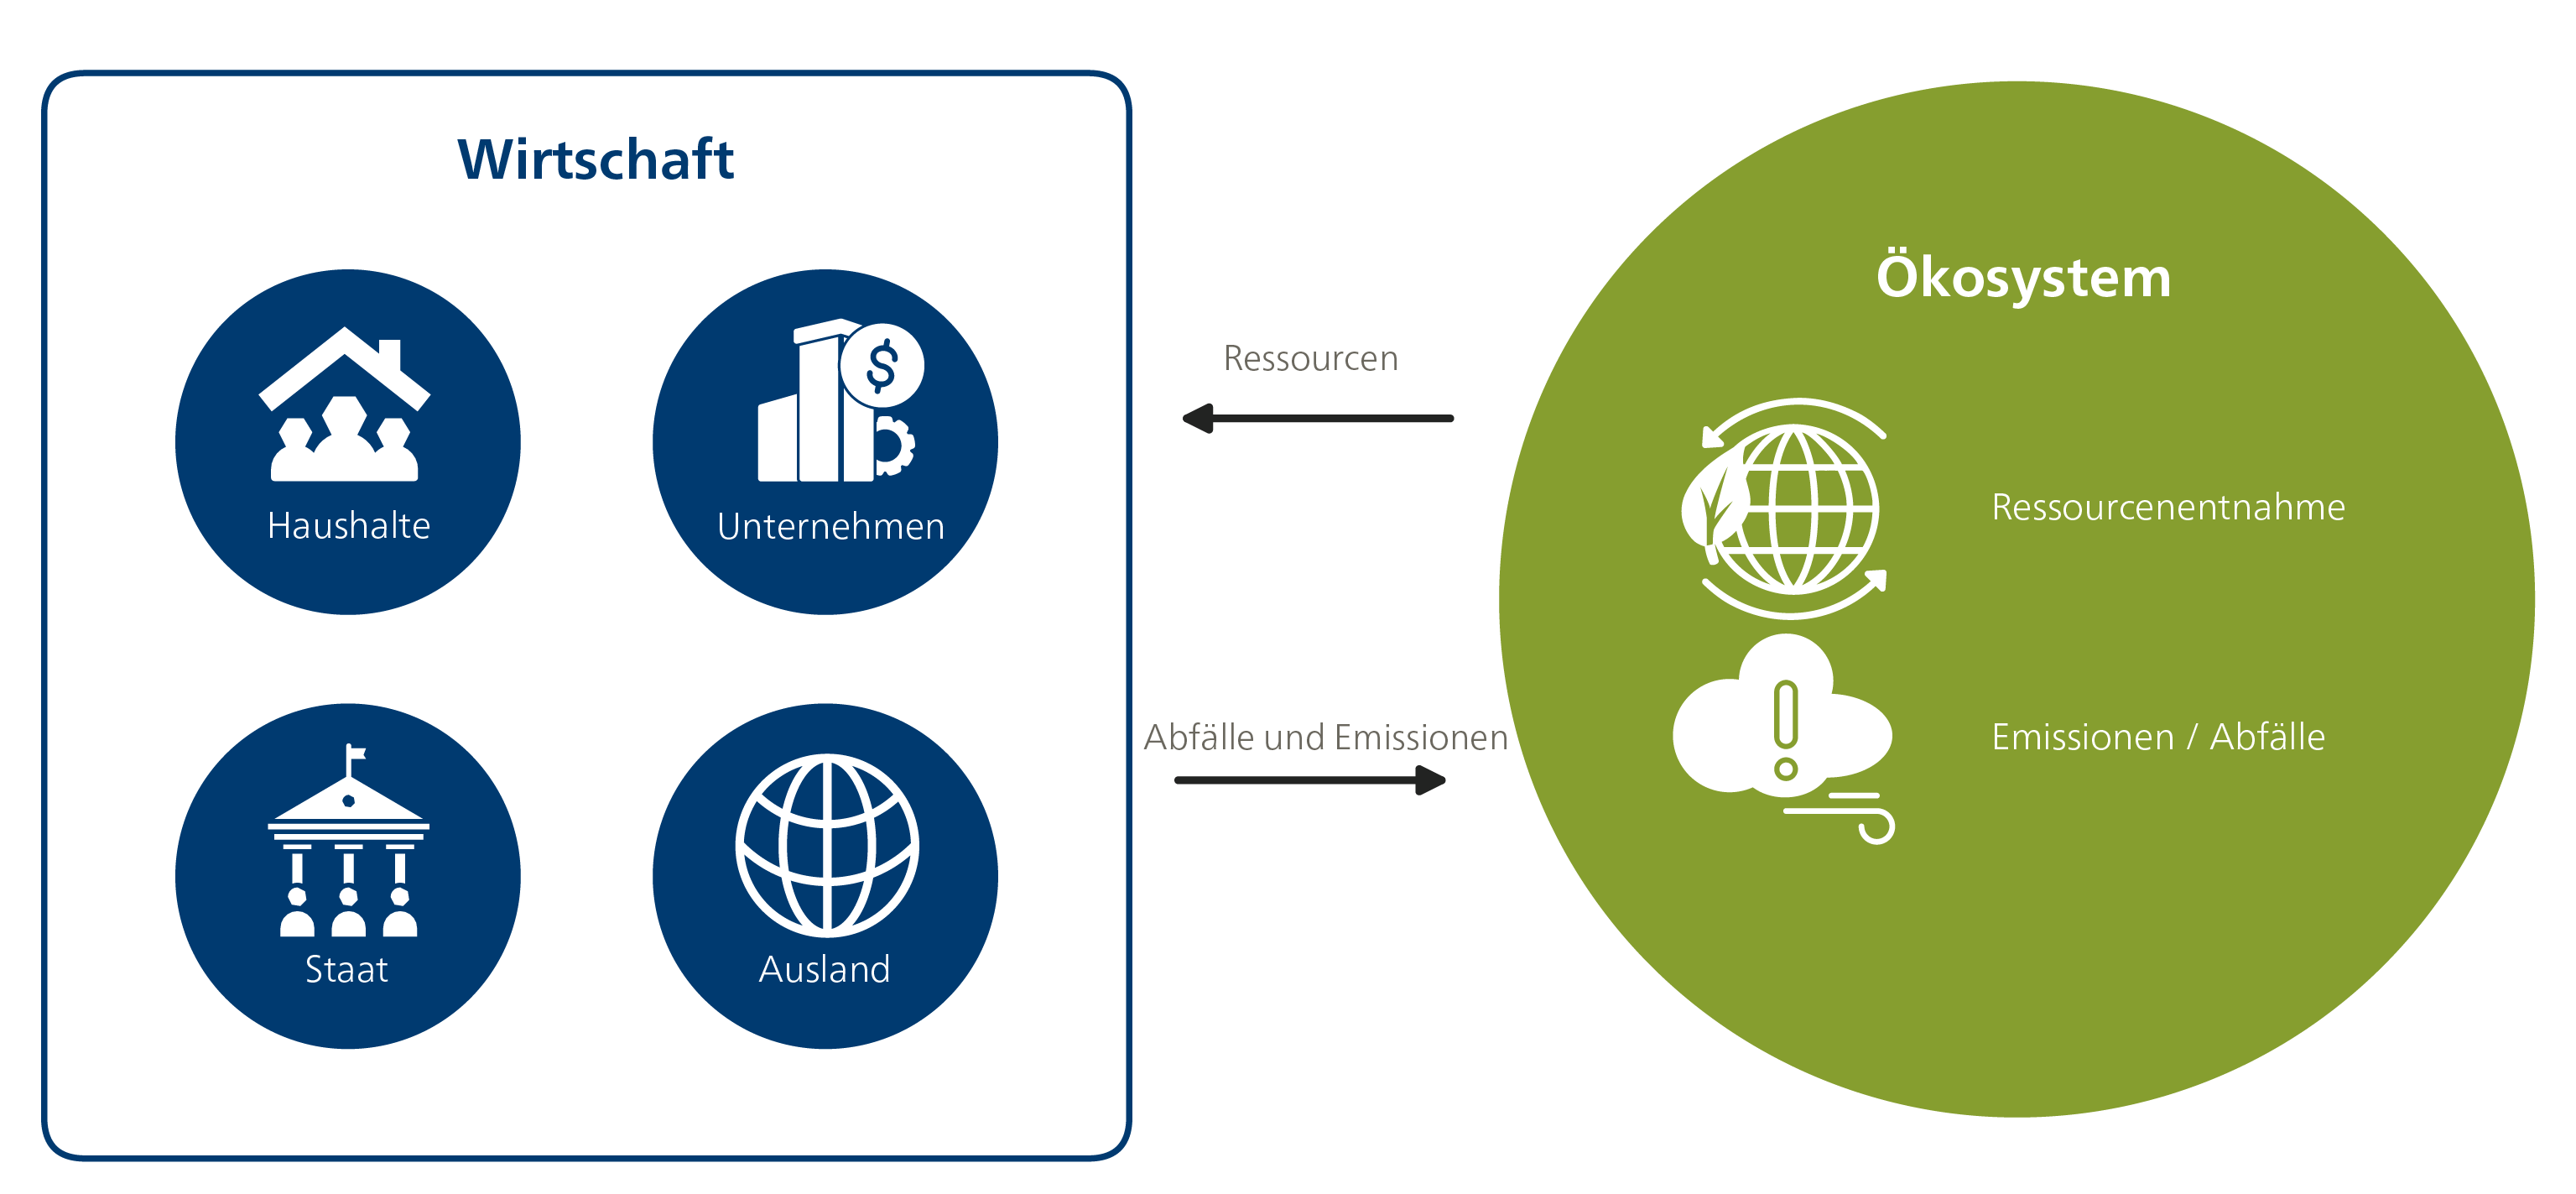
\includegraphics[keepaspectratio]{3_problem-analysis/images/fig3.png}}

}

\caption{\label{fig-econ-nature}Economy and nature as two separate
spheres. Source: Own illustration,
\href{images/fig3_CREDITS_NounProjectIcons.md}{icons from Noun
Project}.}

\end{figure}%

A fundamentally different understanding emerges for ecological
economics. Here, the economy and nature are not conceived side by side,
but the economy is understood as embedded in an ecosystem. The economy
is a subsystem of the global ecosystem and completely dependent on its
functions. All economic activities rely on the extraction of energy and
raw materials from nature and inevitably end in the form of waste and
emissions that are released back into the environment. The economy
therefore cannot be understood independently of the biophysical limits
of the planet. While capital, labour, or knowledge can be increased, the
Earth's resources and its capacity to absorb pollutants are limited.
Figure~\ref{fig-finite-ecosystem} conceptualizes the embedding of the
economic subsystem in a larger finite global ecosystem. The economy is
thus embedded in a finite global ecosystem, draws energy and resources
from it (source function), and also releases matter and energy back into
this ecosystem (sink function). Only solar energy newly enters the
system from outside, while waste heat leaves the Earth at the same time.

\begin{figure}[H]

\centering{

\pandocbounded{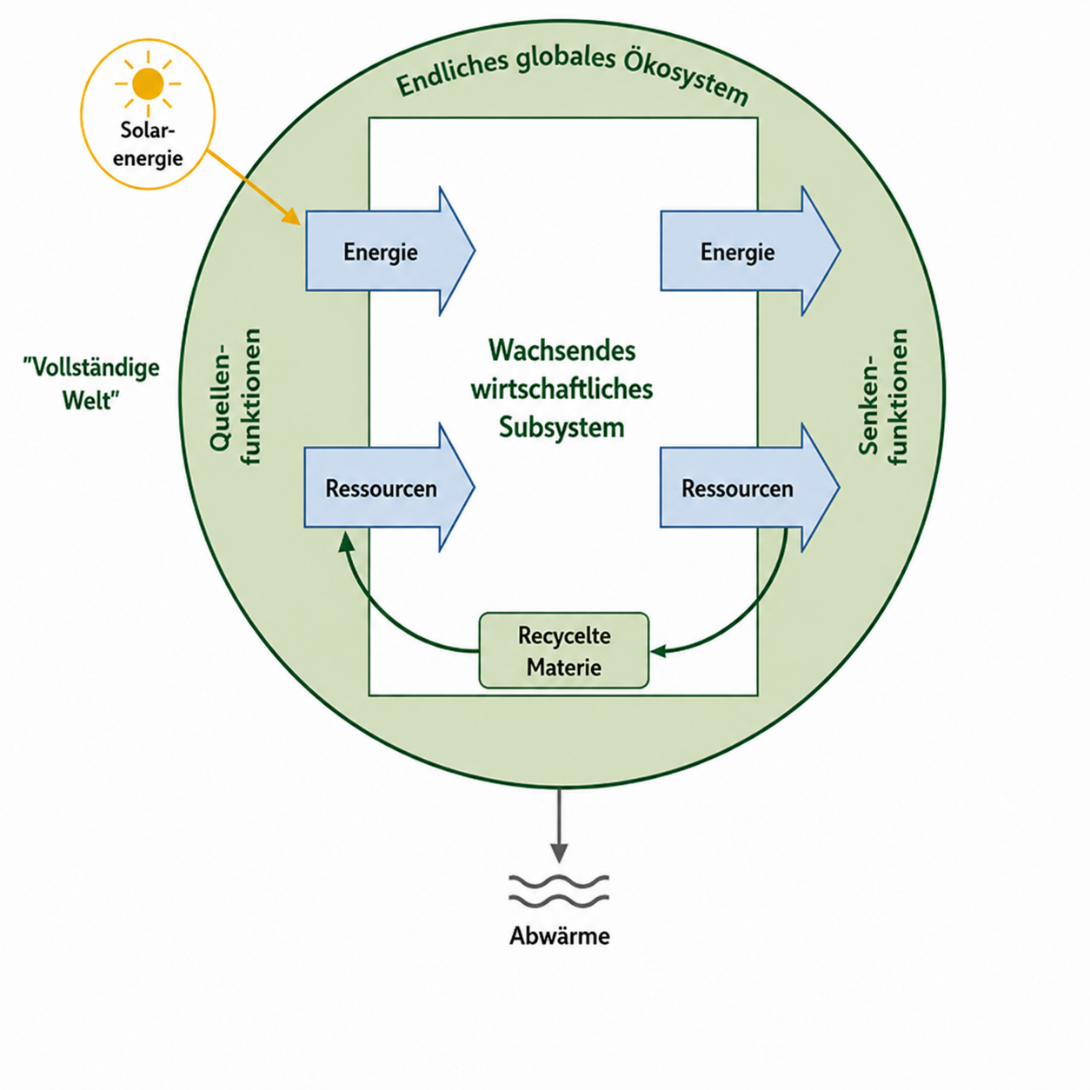
\includegraphics[keepaspectratio]{3_problem-analysis/images/fig4.png}}

}

\caption{\label{fig-finite-ecosystem}Economy embedded in a finite
ecosystem. Source: Own illustration.}

\end{figure}%

These fundamentally different understandings have important consequences
for how we can understand sustainability. The concept of sustainability
can be placed on a continuum from weak to strong (see
Figure~\ref{fig-strong-weak-sustainability}). While the neoclassical
understanding entails a weak understanding of sustainability, ecological
economics has a strong understanding of sustainability. In what follows,
we go into the two understandings.

\begin{figure}[H]

\centering{

\pandocbounded{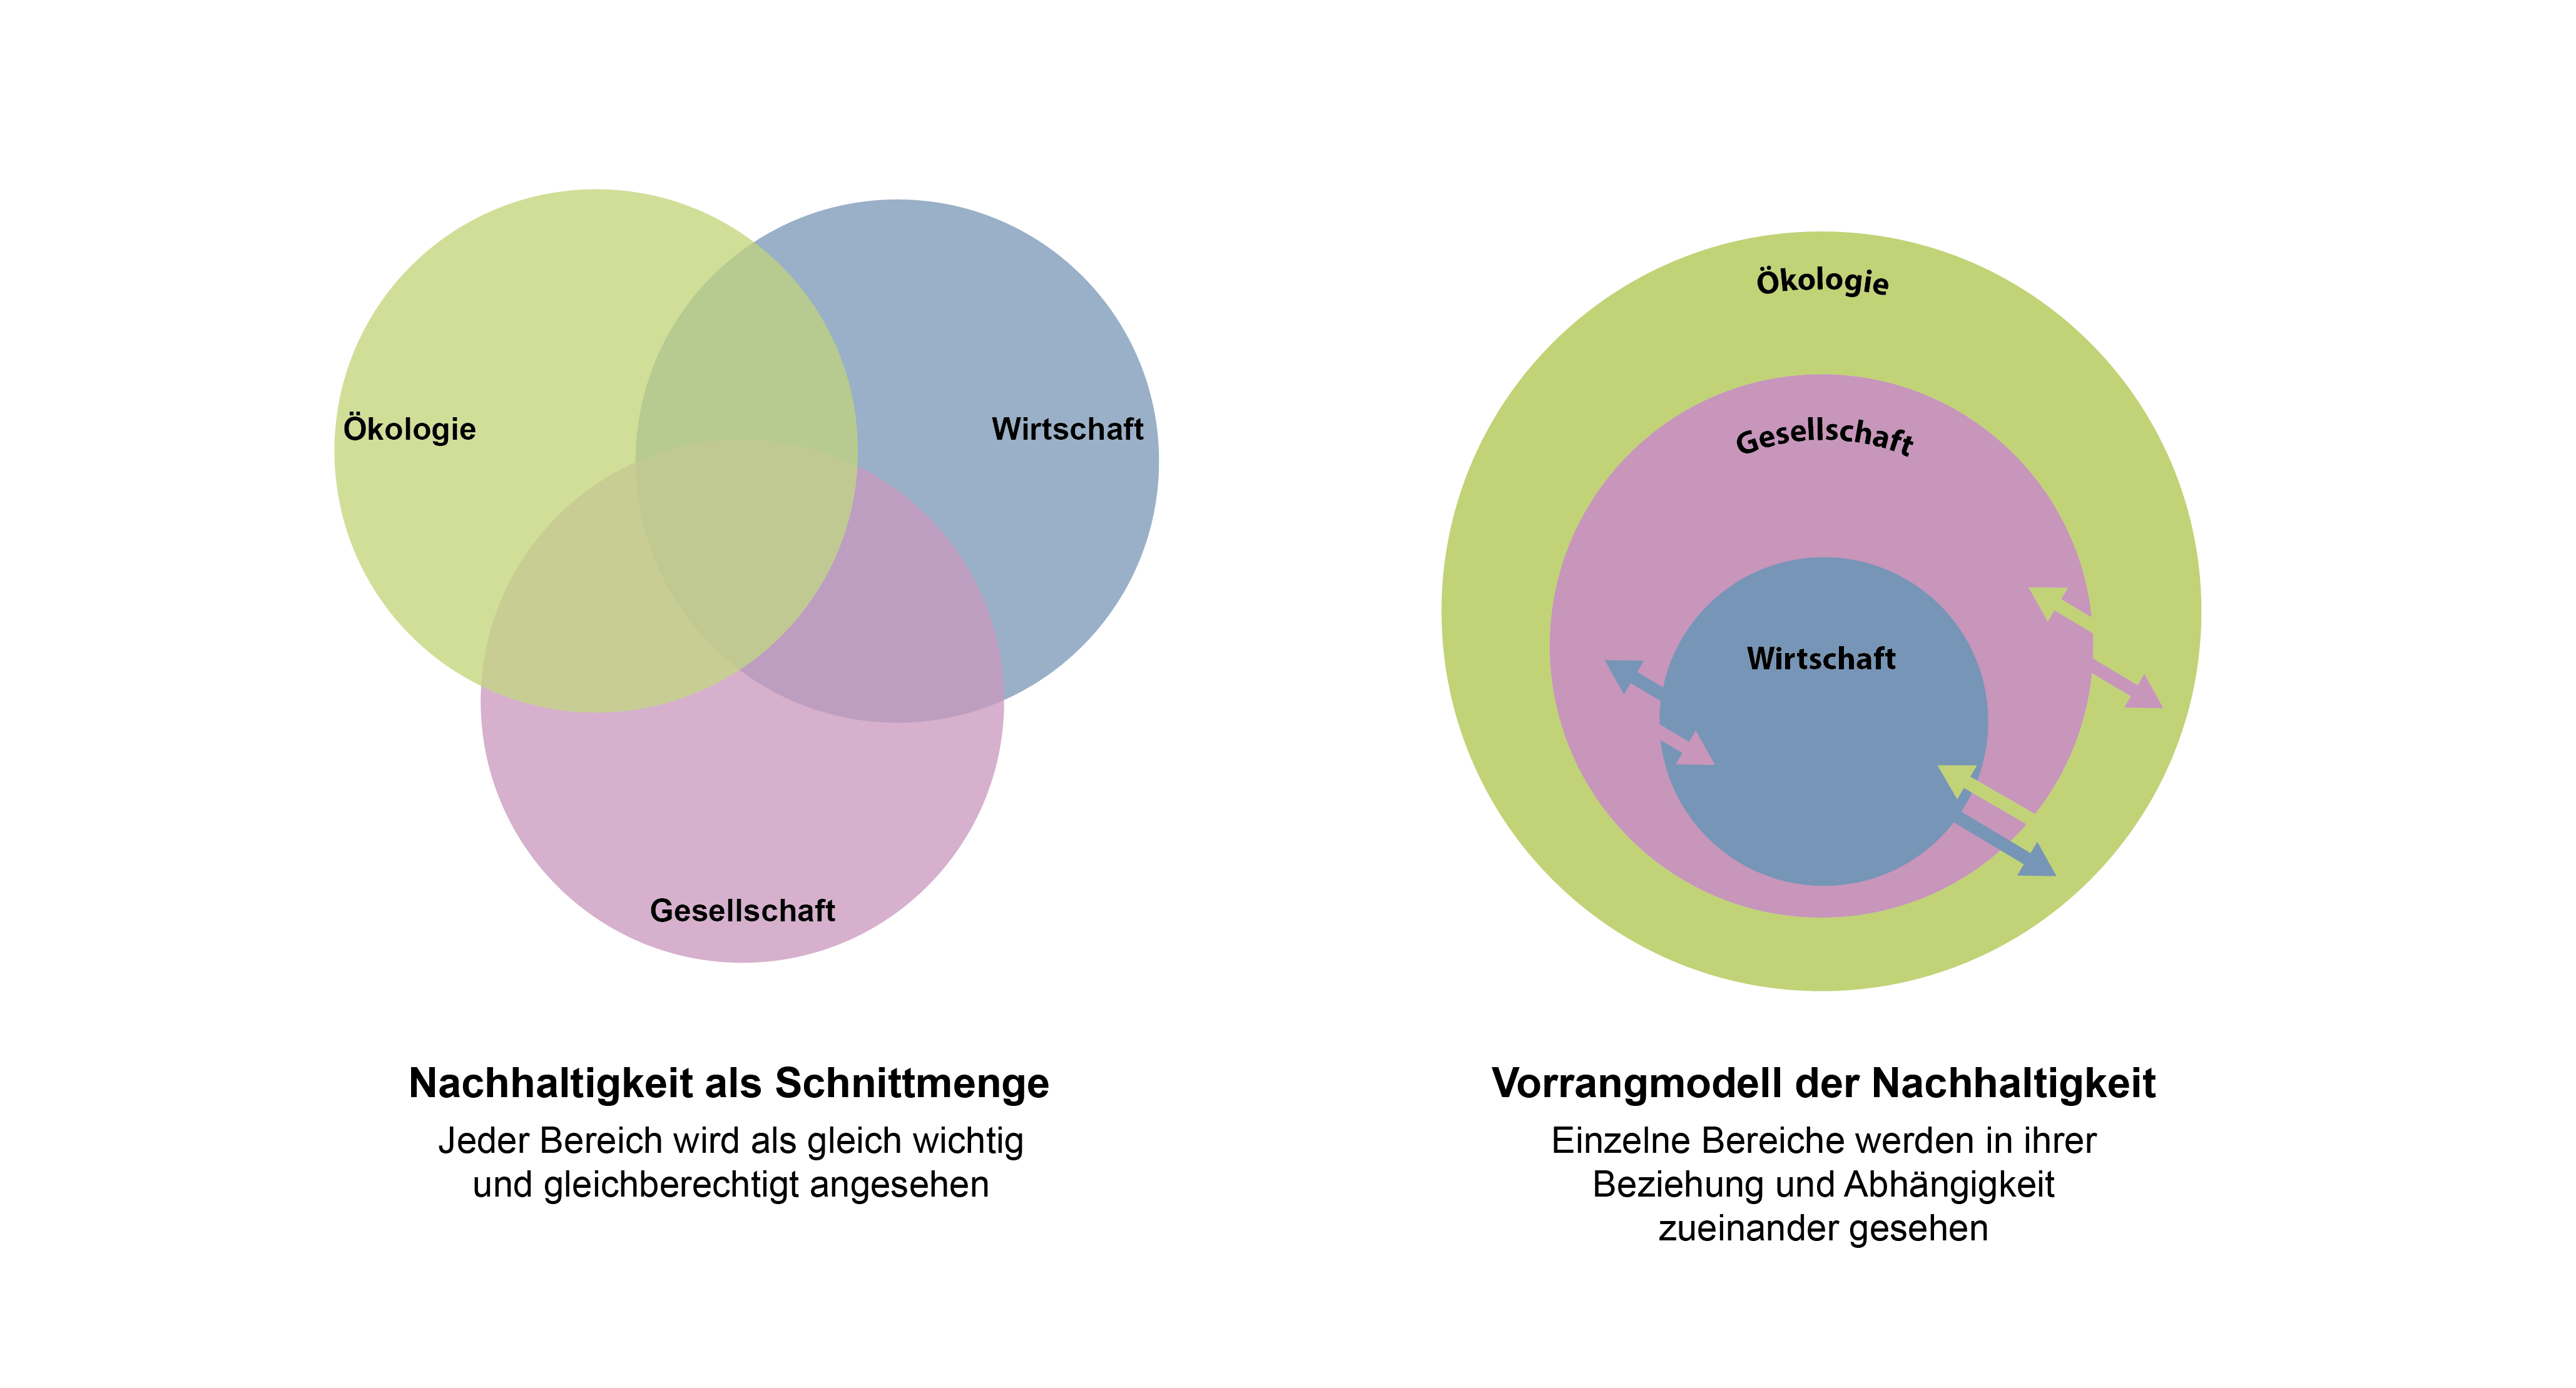
\includegraphics[keepaspectratio]{3_problem-analysis/images/fig5.png}}

}

\caption{\label{fig-strong-weak-sustainability}Weak (left) and strong
(right) sustainability. Source: Own illustration.}

\end{figure}%

\subsubsection[Weak sustainability -- the neoclassical
position]{\texorpdfstring{Weak sustainability -- the neoclassical
position\footnote{Excerpt from Pufé (2017, 105ff.) and
  \url{https://thesustainablepeople.com/starke-und-schwache-nachhaltigkeit/}
  (in German).}}{Weak sustainability -- the neoclassical position}}\label{weak-sustainability-the-neoclassical-position3_intro-1}

Weak sustainability sets a rather ``lenient'' requirement for
sustainability. For the proponents of this view, an action is
sustainable if it offers an advantage to the overall system or at least
does not diminish its quality. Weak sustainability can therefore be
regarded as a kind of basic requirement for sustainability, with the aim
of maintaining a certain level of well-being or quality of life or of
ensuring equality. The concept of weak sustainability ``assumes the
far-reaching and, at least in principle, unlimited {[}\ldots{]}
substitutability of all kinds of capital'' (our translation of Ott and
Döring 2004, 41) and is thus based on the premise of neoclassical
economics, which conceives the different spheres as standing side by
side with equal standing. Natural capital, for example, can be replaced
by other capital; the loss of biodiversity, for instance, could be
replaced by technological capital. It is assumed that it is ultimately
irrelevant in what physical composition the inherited capital stock is
passed on to the next generation -- what matters is only that total
capital and total utility, and thus the overall level of welfare, are
maintained. The concept of weak sustainability builds on neoclassical
utility theory, according to which it is irrelevant how utility is
generated. Environmental economics, which emerged from neoclassical
economics, fundamentally draws on the concept of weak sustainability.

Within the concept of weak sustainability, a measure can nevertheless be
regarded as sustainable even if it comes at the expense of natural
capital. This is the case, for example, if the loss is compensated by an
increase in human or manufactured capital. The extraction of raw
materials such as coal or excessive crude oil production could
accordingly be quite defensible. This understanding tends to recognize
the strong role of technological progress for sustainable development.
Assessing measures on the basis of such a concept is naturally complex,
since it is always tied to many assumptions. Apart from fundamental
questions about sustainability such as ``What is a good life? How is the
level of prosperity measured?'', this approach requires that the value
of the different types of capital be determined. In practice, this means
that a monetary value is attributed to everything. As we saw in Chapter
2.3.1 on land, this is an important prerequisite for substitutability.
It makes the different types of capital comparable and interchangeable.
Even where there is no market price, a monetary value must therefore be
set. Whether such monetary valuation is possible or sensible is
discussed again and again. On the one hand, there is the question of
whether we can give nature a price; on the other, monetary valuation
necessarily implies the substitutability of the natural environment. As
early as 1974, William Kapp doubted whether this monetary valuation
manages to capture the substantial social value that is actually at
stake (Kapp 1974). In addition, fundamental and normative questions
arise in operationalization. Which factors are then taken into account?
What is the value of the beauty of nature? What is the value of a rare
bird or a whale? This short
\href{https://www.youtube.com/watch?v=MSxIBYOMQOU}{video} gives insights
into such questions. Monetary valuation then forms the basis for
cost-benefit analyses, in which, for example, the costs of a climate
measure are weighed against its benefits. In the excursus further below,
you will find, if you are interested, the opportunity to dive somewhat
deeper into this topic.

\subsubsection{Strong sustainability -- the ecological economics
position}\label{strong-sustainability-the-ecological-economics-position}

In contrast to weak sustainability, the strong sustainability position
regards the value of natural capital as irreplaceable. Characteristic of
the proponents of the strong concept of sustainability is that their
optimism regarding the individual possibilities of substitution is
considerably lower. They therefore emphasize the importance of an intact
``natural capital stock''. That the natural capital stock could be
drastically reduced in favour of another type of capital is unthinkable
to them. Human-made capital and natural capital are interchangeable only
to a limited extent. Proponents of strong sustainability thus start from
an ecocentric view, in contrast to the anthropocentric view of weak
sustainability.

In contrast to the confidence of neoclassical economists regarding
substitutability, advocates of strong sustainability do not believe in
solutions based on remediation and reaction but rely on prevention and
anticipation. For example, the growth of the ozone hole can be
compensated only to a limited extent by measures such as sunscreen,
protective clothing, and medical aftercare. Even technological
approaches such as geoengineering are viewed critically, since they
treat the problem superficially instead of addressing its causes.
Geoengineering refers to technical interventions in geochemical or
biogeochemical cycles in order, for example, to slow climate change or
ocean acidification.

So far, the reduction of environmental pressures has mainly concentrated
on end-of-pipe technologies, such as flue-gas cleaning systems on
factory chimneys or catalytic converters in cars. At the same time,
long-term environmental problems were pushed into the background by such
measures as long as their effects were not perceived clearly enough, as
in the case of climate change or the loss of biodiversity. This apparent
protection of the environment is explained by the concept of
\textbf{externalization}, in which environmental and social costs are
shifted outwards, as described, for example, by Lessenich (2018). This
means that pricing takes into account only macroeconomic and
business-economic costs, partly because these are easier to quantify,
while the social and ecological costs of providing goods and services
are left out or shifted outwards. This leads to distortions in market
prices.

\subsection{Climate crisis -- market failure or systemic
problem}\label{climate-crisis-market-failure-or-systemic-problem}

As explained above, climate change concerns one of the central planetary
boundaries and is probably one of the greatest societal challenges of
this century. Although all schools of economic thought recognize the
climate crisis as a central problem, they differ greatly in how they
understand and explain it and in what policy measures can be derived
from it. While neoclassical economics sees the climate crisis above all
as a major market failure, which can be solved by creating a functioning
market, ecological economics, for example, sees the problem more
fundamentally in the capitalist mode of production, that is, in the way
we do business. In what follows, we look at the two understandings using
climate change as an example. Such a juxtaposition could be applied in a
similar way to many ecological crises, for example biodiversity loss,
since the underlying differences lie in the understanding of the
fundamental nature-economy relationship.

\subsubsection{Climate change as market
failure}\label{climate-change-as-market-failure}

From the perspective of neoclassical economics, the climate crisis is
first and foremost a market failure. As explained in Chapter 2.5.2
(\emph{The market as central coordinating mechanism}), markets are
fundamentally regarded as efficient institutions for coordinating
economic activities. Under certain conditions (perfect competition),
they ensure that resources are used where they create the greatest
societal benefit. Since the price mechanism is central to the
functioning of markets, an important prerequisite for this is that all
costs and benefits of an economic action are reflected in market prices.
If this is not the case, the price mechanism cannot function optimally.

And this is exactly the case with the climate crisis. Through the
emission of greenhouse gases, companies and households cause costs that
are borne not by themselves but by society. These costs are not
automatically included in the market price of goods. Such consequences
not included in the market price are called negative externalities (see
Chapter 2.4.2, \emph{External effects -- why does a flight often cost
less than a train ride?}). The costs of climate change -- such as
extreme weather events, crop failures, or biodiversity losses -- are
therefore not fully reflected in the prices of fossil fuels. Fossil
energy appears artificially cheap, which produces more emissions than
would be desirable for society. This is shown in
Figure~\ref{fig-welfare-loss}. The dashed red line would correspond to
the social marginal costs, and the solid red line corresponds to the
private marginal costs. Since only the private costs are reflected in
the price, the price of goods based on fossil fuels is too low, and
accordingly the quantity at market equilibrium A is too high.
Concretely, this means that the quantity of CO\textsubscript{2} emitted
is too high. If all social costs were reflected in the price, the
optimal market equilibrium would be at point B with a quantity y*. The
grey triangle denotes the overall economic welfare loss caused by these
negative externalities.

As hinted in Chapter 2.5.2 (\emph{The market as central coordinating
mechanism}) (and set out in more detail in Chapter 5), market failure
is, in neoclassical economics, a reason for the state to intervene.
According to this analysis, the central economic policy task is now to
internalize these external costs. This means that all costs and benefits
are integrated into the price. The polluter-pays principle (that is,
that the costs are borne by those who cause them) is to be restored by
putting a price on emissions. The most important instruments include
CO\textsubscript{2} taxes or emissions trading systems, in which
CO\textsubscript{2} emissions receive a price and are traded via a
market. Both approaches aim to raise the price of fossil fuels and
thereby create incentives for lower-emission technologies, innovation,
and behavioural change. Companies and households then decide for
themselves how they reduce their emissions at the lowest cost. From a
neoclassical perspective, market-based instruments therefore enable
efficient climate protection at the lowest possible overall economic
cost, since in this way we move to the optimal equilibrium point B. This
approach requires the substitutability from weak sustainability and that
it is possible to put a price on all costs and benefits (for example the
loss of biodiversity), as explained before.

\begin{figure}[H]

\centering{

\pandocbounded{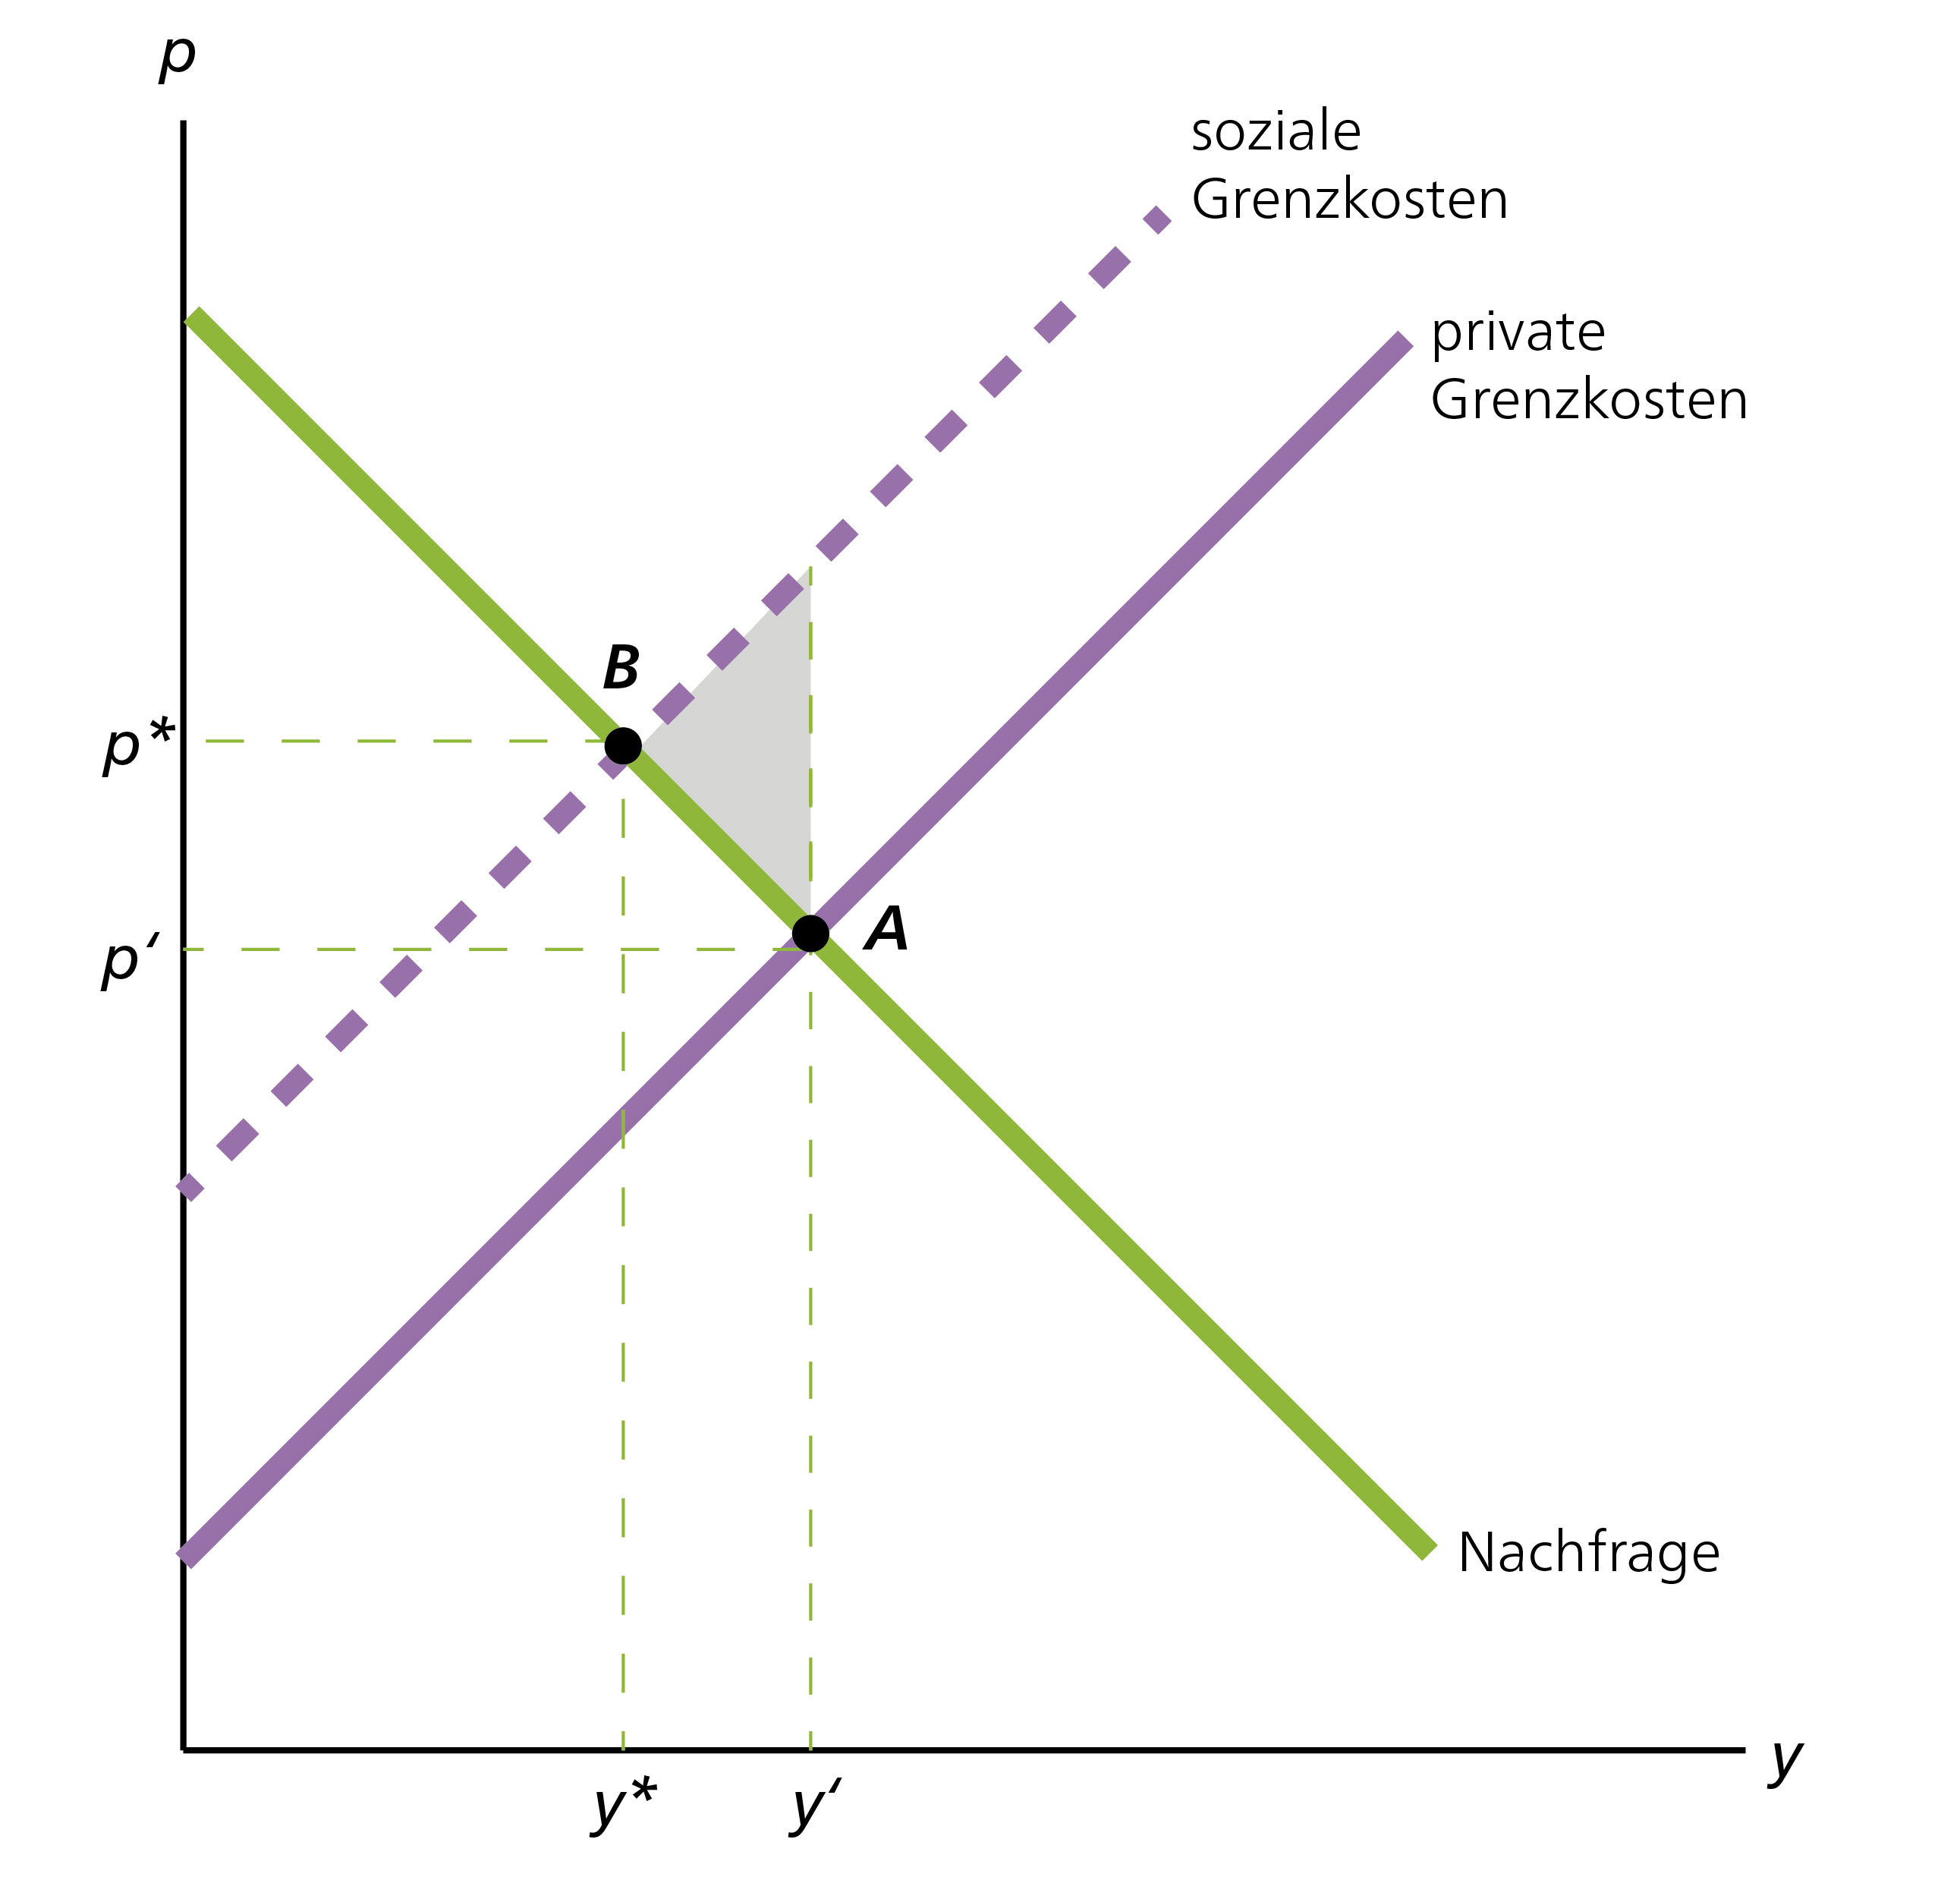
\includegraphics[keepaspectratio]{3_problem-analysis/images/fig6.png}}

}

\caption{\label{fig-welfare-loss}Welfare loss (grey triangle) with
external costs. Source: Own illustration.}

\end{figure}%

In this approach, fundamental structures are taken as given, and
accordingly the fundamental economic order is not called into question.
Markets continue to be regarded as a suitable mechanism for allocating
resources; they merely have to be corrected where market failure occurs.
Economic growth is accordingly not regarded as a problem. Rather, it is
assumed that, with functioning markets, price signals, technological
progress, and innovation can lead in the long term to a decoupling of
economic growth and environmental pressure.

\subsubsection{Climate change as systemic
problem}\label{climate-change-as-systemic-problem}

Ecological economics does share the assessment that environmental costs
are often externalized, but it interprets the climate crisis in a
fundamentally different way. It regards climate change not merely as a
market failure but as a symptom of an economic system that is based on
permanently rising material and energy throughput and thereby exceeds
the planetary boundaries of the Earth.

The starting point here is the understanding, discussed several times,
that the economy is not an independent system. Against this background,
the climate crisis appears not as an isolated environmental problem but
as an expression of fundamental tensions between economic development
and the ecological carrying-capacity limits of the Earth system. Climate
change is thus closely linked to other ecological crises -- such as the
loss of biodiversity, the overuse of natural resources, or the
disruption of biogeochemical cycles. The various environmental problems
are understood as interconnected symptoms of an economic system whose
material and energy throughput is continually growing.

In contrast to neoclassical economics, ecological economics therefore
does not understand environmental problems primarily as the result of
missing market prices. The idea of negative externalities is not
rejected, however. But these are not regarded as an exception in an
otherwise functioning market; they are regarded as a structural feature
of capitalist modes of production. Companies compete with one another
and strive to keep production costs as low as possible. As long as a
system is based on maximizing private profit, there is an incentive to
shift costs onto people, society, and nature, that is, to externalize
them (Kapp 1950; Saave and Jena 2022). The externalization of ecological
costs is therefore not a random market failure but is understood as an
inherent consequence of the growth and competition logic of capitalist
economic systems.

Beyond this, ecological economics emphasizes the particular significance
of economic growth. Historically, the growth of gross domestic product
went hand in hand almost everywhere with rising consumption of energy
and materials. Although the resource and energy intensity of many
production processes has fallen, these efficiency gains were often
overcompensated by the growth of production and consumption. For
ecological economics, what is decisive is therefore not only how
efficiently resources are used but whether absolute resource and energy
consumption stays within the planetary boundaries.

In this context, it distinguishes between relative and absolute
decoupling from economic growth. Relative decoupling is said to occur
when resource consumption or emissions grow more slowly than gross
domestic product. Absolute decoupling, by contrast, occurs only when
environmental pressure actually falls despite continued economic growth
(see Figure~\ref{fig-decoupling}).

\begin{figure}[H]

\centering{

\pandocbounded{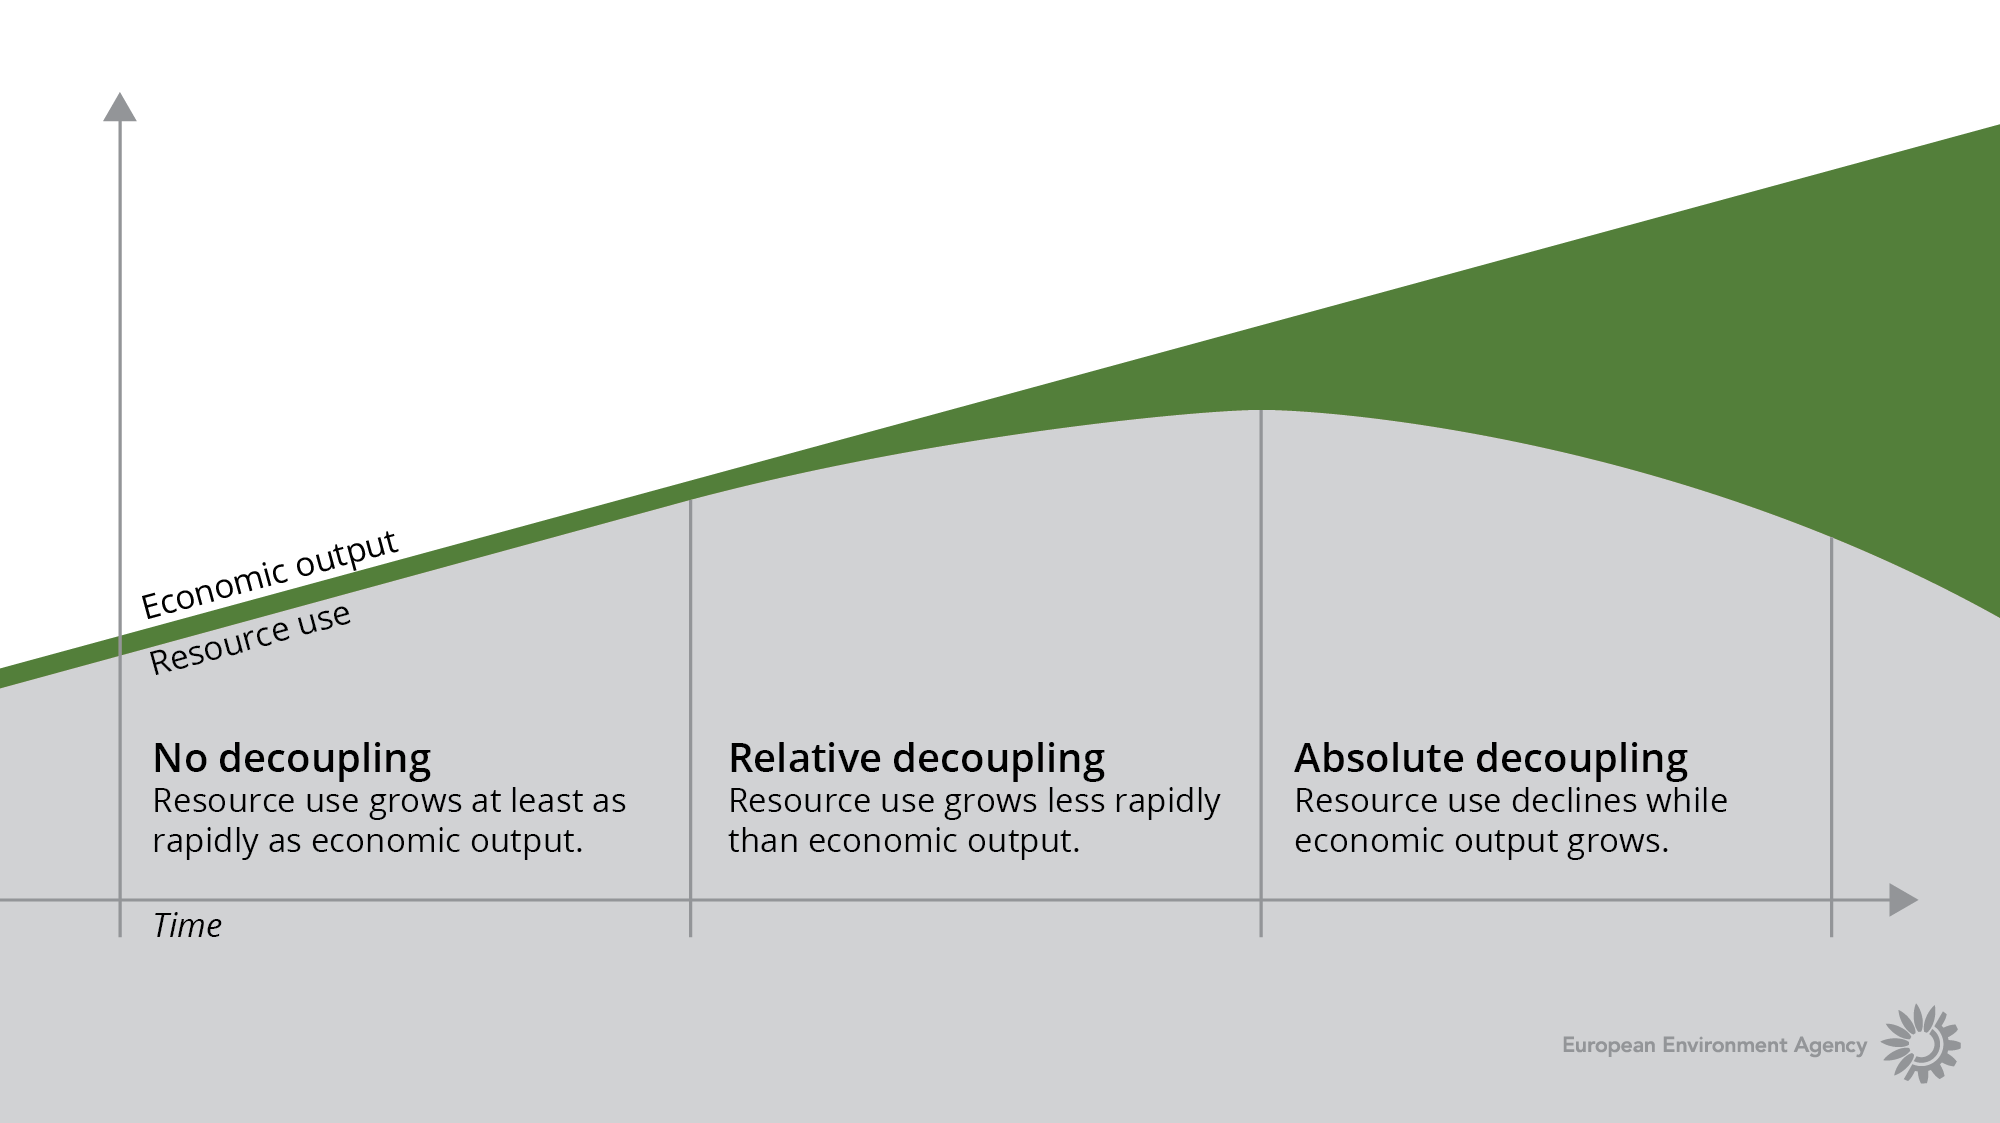
\includegraphics[keepaspectratio]{3_problem-analysis/images/fig7.png}}

}

\caption{\label{fig-decoupling}Relative and absolute decoupling; Source:
EEA (2015).}

\end{figure}%

While relative decoupling can be observed in many countries, proponents
of ecological economics are sceptical about the possibility of lasting
absolute decoupling on the scale required globally. Part of the observed
emission reductions in industrialized countries is also based on the
relocation of resource-intensive production to other regions of the
world rather than on an actual reduction of global material and energy
consumption. As shown in Figure~\ref{fig-absolute-decoupling}, absolute
decoupling can be observed in some countries of the Global North
(although not all emissions are included). This concerns, however, not
resource consumption but only CO\textsubscript{2} emissions, and it
remains questionable whether this is possible at the global level. At
the global level, no absolute decoupling of CO\textsubscript{2}
emissions and economic growth can be observed.

\begin{figure}[H]

\centering{

\pandocbounded{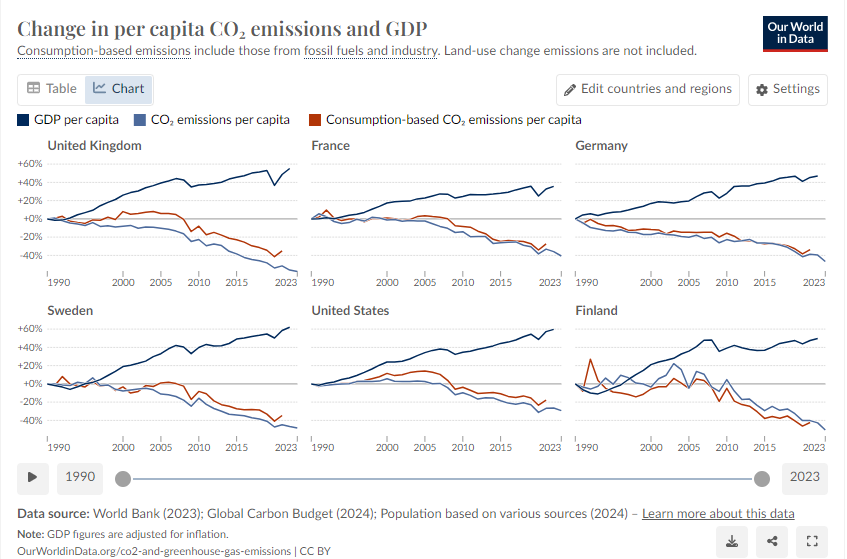
\includegraphics[keepaspectratio]{3_problem-analysis/images/fig8.png}}

}

\caption{\label{fig-absolute-decoupling}Absolute decoupling in selected
industrialized countries. Source: Global Carbon Budget (2025);
population figures based on various sources (2024) -- with extensive
data processing by Our World in Data.}

\end{figure}%

Another important point is the discussion on \emph{rebound effects}.
Technological innovations often increase the efficiency of resource use
but thereby often make products and services cheaper. Falling costs can
in turn lead to greater demand, so that part of the originally expected
environmental relief is lost again. Modern vehicles, for example,
consume less fuel per kilometre than earlier models, but at the same
time the lower costs can lead to larger vehicles being bought or more
distance being travelled, which constitutes direct rebound effects.
Indirect effects would occur here, for example, if the lower costs lead
to more air travel on holidays, which can then also lead to higher
energy consumption (see Figure~\ref{fig-rebound-effect}).
Energy-efficient household appliances or buildings, too, do not
automatically lead to a correspondingly lower energy consumption. From
the perspective of ecological economics, efficiency improvements are
therefore indispensable, but they alone are not sufficient to reduce
absolute resource consumption sufficiently.

\begin{figure}[H]

\centering{

\pandocbounded{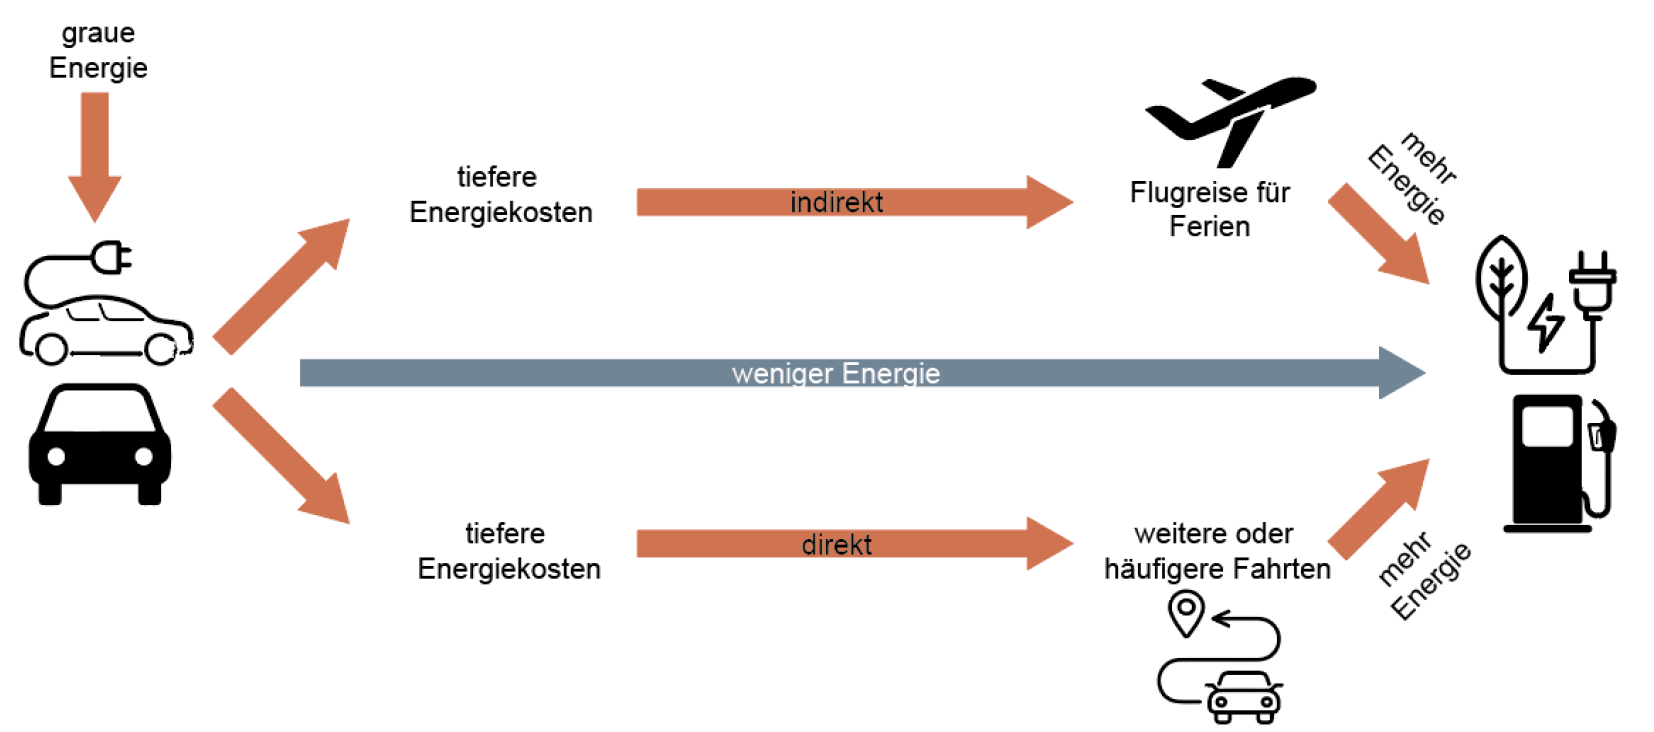
\includegraphics[keepaspectratio]{3_problem-analysis/images/fig9.png}}

}

\caption{\label{fig-rebound-effect}Indirect and direct rebound effects
of energy-saving passenger cars. Source: Own illustration.}

\end{figure}%

The problem analysis of ecological economics leads to different policy
conclusions than in neoclassical economics. It is also important to
emphasize, however, that the internalization of external costs through
CO\textsubscript{2} prices or emissions trading is not rejected in
principle; it is regarded merely as one building block of a more
comprehensive transformation. Contrary to the neoclassical perspective,
the economic system is fundamentally called into question here, and
solutions also include fundamental transformations of the existing
system. In self-study phase 6, we will look more closely at various
possible approaches that follow from an analysis of strong
sustainability, but also at those that are more oriented towards a
neoclassical understanding. In many sustainability debates, the
differences lie at their core in these fundamental differences.

\begin{tcolorbox}[enhanced jigsaw, arc=.35mm, bottomrule=.15mm, bottomtitle=1mm, breakable, colback=white, colbacktitle=quarto-callout-tip-color!10!white, colframe=quarto-callout-tip-color-frame, coltitle=black, left=2mm, leftrule=.75mm, opacityback=0, opacitybacktitle=0.6, rightrule=.15mm, title={Excursus -- Cost-benefit analysis}, titlerule=0mm, toprule=.15mm, toptitle=1mm]

Cost-benefit analysis makes it possible to weigh costs against benefits.
This instrument makes it possible to evaluate the expected consequences
of decisions by weighing the associated costs and benefits. The
important precondition of this analysis is the monetary valuation of all
consequences. Only in this way can an evaluation be made with comparable
quantities. The establishment of cost-benefit analysis goes back to the
discussion of social costs (external costs) in the 1950s and 1960s.
Based on the work of economists such as William Kapp (1950), it was
argued that the social costs that arise should be prevented through
regulation. Ronald Coase (1960), by contrast, argued that regulations,
too, would constitute costs for companies: opportunity costs through
forgone profit. For example, the profit of a chemical company that
pollutes a river through its activity. This profit of the company would
have to be offset against the social costs. According to Coase, such a
total calculation is supposed to provide a basis for arguing against
regulations and for extending property rights (that is, the market).

Cost-benefit analysis has several problems. One difficulty is that the
value of many areas of societal and natural life cannot be clearly
expressed in a price. It is not possible, for example, to put a clear
and objective price on an endangered animal or plant species, the
existence of a forest, clean air, or a human life. To meet this
challenge, researchers have developed various methods intended to make
it possible to quantify monetary values. Two main procedures are
important here: with \textbf{stated preference methods}, actors can be
asked about different future scenarios. Previously unknown circumstances
can thus be weighed against one another. In \textbf{revealed preference
methods}, a utility valuation for the future is derived from decisions
already made. This prevents actors from giving strategic answers when
valuing expected future scenarios. However, conditions that have not
occurred before cannot be valued. Although there are established
procedures for valuing preferences, they are limited in their
possibilities for weighing costs and benefits. As the term
``preference'' already suggests, these are always subjective views. The
monetary valuation derived from them will therefore also always be
subjective, that is, not an objective number.

\textbf{Example:}\\
At the beginning of this millennium, it emerged that the tobacco company
Philip Morris had commissioned a cost-benefit analysis in the Czech
Republic on the effects of smoking on the country. The authors concluded
that smoking made an annual profit of about 5.8 billion crowns (about
USD 150 million) for the Czech state budget. Because of the lower life
expectancy of smokers, the state has to provide for them for a shorter
time and therefore saves money. This report triggered a public outcry,
whereupon the tobacco company apologized. But this example also shows
the subjective nature of cost-benefit analysis. By reducing the value of
human years of life to a number, the company had not only crossed a
moral line. As a scientist later showed, the company had also made false
assumptions and left out wider-reaching costs in the report. Her
cost-benefit analysis of the same scenario concluded that smoking in the
Czech Republic contributed to an annual deficit of about 14 billion
crowns.

A further problem is that a cost-benefit analysis implies that the
different types of capital are substitutable for one another, that is,
that the loss of biodiversity, for example, can be technologically
substituted. We discussed this problem in detail in this chapter.

\textbf{Discounting -- the time factor}

The time factor is included in cost-benefit analysis by means of
\emph{discounting}. This means that costs incurred in the future are
valued as smaller. The discount rate influences how strongly perceived
costs decrease with the passage of time. Various decision bases can be
used to determine the discount rate. Intergenerational justice, the
decision between strong and weak sustainability, the uncertainty of
future events, or the time preference of the decision-makers influence
how strongly future costs are discounted.

\begin{figure}[H]

\centering{

\pandocbounded{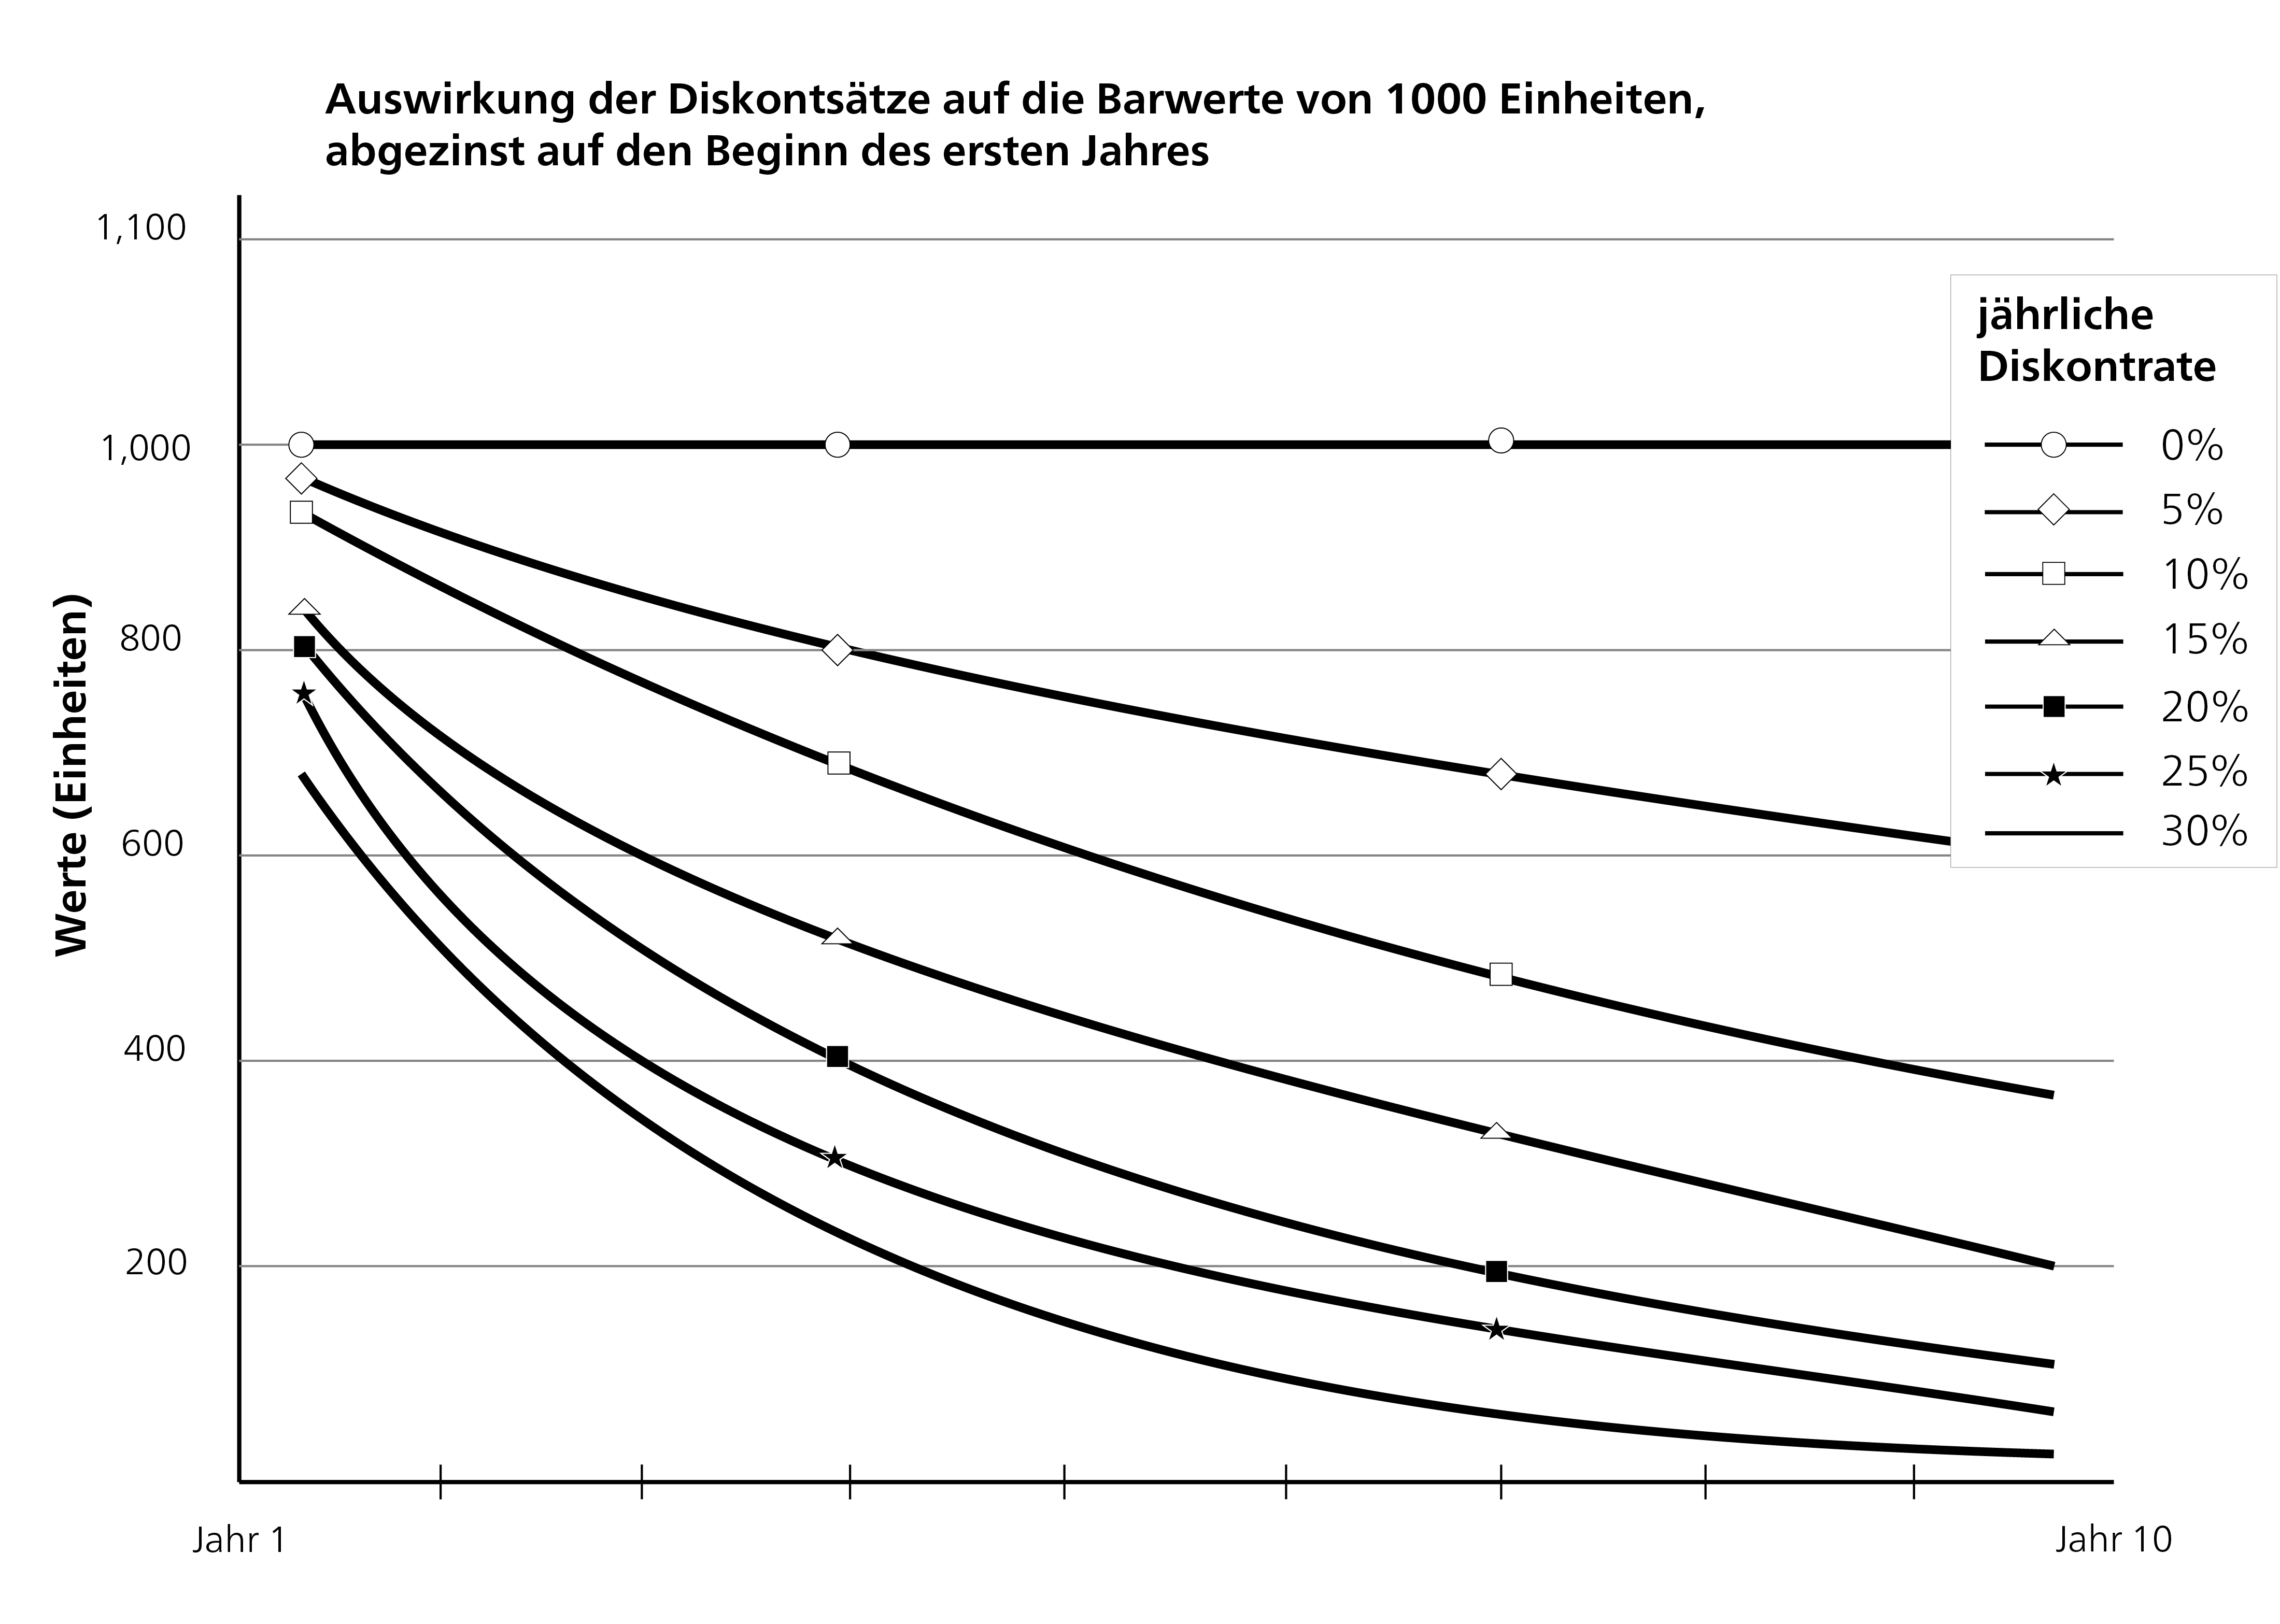
\includegraphics[keepaspectratio]{3_problem-analysis/images/fig10.png}}

}

\caption{\label{fig-discount-rates}Illustration of different discount
rates over time.}

\end{figure}%

Figure~\ref{fig-discount-rates} shows different discount rates over the
same period. The costs of climate damage of CHF 1,000 occurring in 15
years, for example, are valued at about CHF 800 at a discount rate of
1.5\%. At a rate of 5\%, only about CHF 460 are included as perceived
costs in the cost-benefit calculation.

\textbf{Example:}\\
In 2006, the British economist Nicholas Stern published the so-called
\href{https://webarchive.nationalarchives.gov.uk/ukgwa/20100407172811/https:/www.hm-treasury.gov.uk/stern_review_report.htm}{Stern
Report} on behalf of the British government. In this comprehensive
document, he describes climate change as the greatest market failure in
history and argues by means of cost-benefit analysis that one per cent
(later he argued for two per cent) of global GDP must be invested in
emission reduction. Economists reacted to Stern's report in mixed ways.
While some supported it, others argued that he calculated the costs of
global warming incorrectly. The main argument was his low discount rate
of 0.1 per cent, which he used to value future costs. The economist
William Nordhaus took over Stern's calculations and changed only the
discount rate from 0.1\% to 3\%. Accordingly, investments against global
warming are still necessary but considerably lower than Stern demanded.
In the logic of cost-benefit analysis, Nordhaus concludes that global
warming in the optimal scenario rises to more than 3 degrees by 2100
(Nordhaus 2019). In this example, the question of the discount rate
constitutes a clear ethical positioning. Stern chose the rate of 0.1\%.
He argues that future generations should not be given less weight
because of their later point in time. The discount of 0.1 represents the
low risk that humanity is wiped out by a catastrophic event. Nordhaus's
discount rate, by contrast, weights the welfare of coming generations by
3\% less with each year. This is on the assumption that the economy
grows continuously at this rate and future generations will accordingly
be wealthier, and the costs will weigh less in the future.

The calculation of costs and benefits in the future thus depends on many
assumptions and ethical questions. These are meant to be represented
numerically in the discount rate.

\end{tcolorbox}

\begin{tcolorbox}[enhanced jigsaw, arc=.35mm, bottomrule=.15mm, bottomtitle=1mm, breakable, colback=white, colbacktitle=quarto-callout-caution-color!10!white, colframe=quarto-callout-caution-color-frame, coltitle=black, left=2mm, leftrule=.75mm, opacityback=0, opacitybacktitle=0.6, rightrule=.15mm, title={Further reading}, titlerule=0mm, toprule=.15mm, toptitle=1mm]

Buller, Adrienne. 2022. \emph{The Value of a Whale: On the Illusions of
Green Capitalism}. Manchester University Press.

\end{tcolorbox}

\section{Social Limits: Is the Pie Growing for Everyone -- or Only for a
Few?}\label{social-limits-is-the-pie-growing-for-everyone-or-only-for-a-few}

\emph{↗ Textbook chapters 8 and 9}

When industrial production in the cities picked up speed in the early
19th century, industrialists needed workers en masse. They ``found''
them through increasing internal migration from rural areas. Through the
advancing \emph{enclosure} and privatization of the commons, a large
part of the rural population increasingly lost its livelihood and had to
migrate to the cities to earn a living there as industrial workers. Only
in this way could industrial production and the capitalist market
economy establish themselves as a new economic and social system. But
the economic upswing by no means benefited all those involved equally:
while factory owners attained unprecedented wealth, growing destitution
prevailed in the new working-class districts. Countless reports testify
to an unprecedented extent of suffering and inhumane conditions, both in
the factories and in the overcrowded barracks of workers' families.
Shifts of 14 to 16 hours without breaks, child labour, and appalling
health risks were the bleak norm. But anyone who insisted on rights
quickly risked their job and thereby pushing their family to the brink
of survival from misery: there was no shortage of labour, and the
hardship was great enough that any conditions had to be accepted.

But criticism of the new conditions, and in particular of human
destitution, also manifested itself early on. Besides the first
self-help associations such as consumer cooperatives, intellectual
responses to the misery of industrial capitalism also increasingly
formed. Various wings of early socialism named the problem of the
dehumanizing conditions (for example, Robert Owen in England). The
objections to the market system were mostly formulated from the
perspective of the working class. People did not want to simply keep
accepting the miserable situation in which wage workers and their
families found themselves. A central endeavour, for example, was the
organization of the workers in cooperative associations that organized
both the production and the distribution of goods according to
principles of a fair wage and concrete need.

In the middle of the 19th century, Karl Marx, a German living in
industrial England, set about writing the most influential critique of
capitalism to this day. Almost a century later, Karl Polanyi (1886-1964)
finally described, from a historical perspective, human misery as a
necessary consequence of a market society. Polanyi described the
\emph{market} of the time as a capitalist market that had slipped away
from any social control and was in this sense ``disembedded''. He
explained his observation by the inclusion of money, labour power, and
land in the market-mediated process of price formation. In his
conviction, only this gave rise to a system of market exchange detached
from all normative restrictions, which tends to destroy all social
obligations, reliabilities, and notions of honour in the lifeworld. At
the same time, according to Polanyi (2017), the complete
\emph{commodification}, and thus the creation of a pure market society,
could nowhere fully prevail, since societies at a certain point take
countermeasures to counteract, for example, the emerging misery and
societal disembedding and alienation (Polanyi 2017). The trade union and
cooperative movement establishing itself towards the end of the 19th and
the beginning of the 20th century, but above all the emerging welfare
state, can, in this reading, be understood as a counter-reaction
inherent in simultaneously advancing capitalism. It has, to a certain
extent, a double function of \emph{limiting} it: to protect people from
its consequences and, at the same time, to protect capitalism from
itself.

\subsection{Social limits in the 21st
century}\label{social-limits-in-the-21st-century}

As Figure~\ref{fig-acceleration} under the ecological limits shows, in
the 20th century not only Earth system trends but also socioeconomic
ones accelerated strongly. Although social progress (or
counter-movements) has noticeably reduced extreme poverty and misery in
many industrialized countries, various social limits worldwide are at
similar risk of being crossed as ecological ones. \emph{Doughnut
Economics}, a well-known book and framework of the same name by the
economist Kate Raworth, accordingly supplements the nine ``planetary
boundaries'' with twelve ``social foundations'' (Raworth 2017). These
include, for example, food security, health care, and access to
education. In a similar way, the 2030 Agenda, adopted by all UN member
states, reflects in its 17 \emph{Sustainable Development Goals} (SDGs)
the continuing urgency of social questions as part of sustainable
development.

Despite this supposedly broad acceptance of the goals, social limits are
often less clear to draw than planetary boundaries and are accordingly
discussed more controversially. As we will see, social questions are
closely tied to ideas of justice and of a good life. The term
``boundary'' is therefore less obvious at first glance, especially in
comparison with the biophysical limits of planetary ecology. On closer
inspection, however, the notion of a social boundary, or a foundation
that must not be fallen short of, makes perfect sense if we understand
society and humanity as a whole as social systems whose functioning --
similar to ecology -- can be thrown out of balance. This can happen
through social as well as primarily economic changes, which moreover
often complement each other. The misery of workers in early capitalism,
for example, was at first glance characterized by material poverty, but
migration to the cities also meant being torn out of the familiar social
environment with all its contacts and rhythms.

Today, too, scientists emphasize social limits that go along with the
ever-recurring need to adapt to constantly new laws of capitalist
economy and society. The German sociologist Hartmut Rosa describes
modernization as a process of ``social acceleration'' (see, for example,
Rosa and Celikates 2024; Rosa 2003). According to Rosa, alongside
technological progress, \textbf{social change}, for example the change
of social relationship patterns, and the \textbf{pace of life} also
accelerate. These acceleration processes are driven by economic,
cultural, and structural factors and mean that, despite constant
technological progress and the associated efficiency gains, we
increasingly feel short of time and stressed. For example, the enormous
advances in communication technology have made it possible for us to
communicate over long distances much more efficiently (for example
emails instead of sending letters). Where we once wrote at most a few
letters, the number of emails sent has increased massively, so that we
fill the freed-up time, to a certain extent, with sending additional
emails, which in turn brings further obligations and changes
relationship patterns. The possibilities and demands of being reachable
have thus increased, for example. With technological progress, the
possibilities of experiencing parts of the world also accelerate, for
example through advances in transport and communication, but also in
completing more and more tasks with the help of artificial intelligence.
The potentially experienceable world grows faster than the share we can
actually experience. Relatively speaking, the share of the world that we
can experience therefore shrinks. Such acceleration dynamics have
effects on the social well-being of individuals and societies and
therefore cannot be disregarded.

A further social limit that increasingly occupies economists (although
by no means all of them) is the growing inequality of income and wealth
in many places and globally. But why can income and wealth inequality be
described as a social limit? The epidemiologists Kate Pickett and
Richard Wilkinson, for example, have shown that social, health, and
environmental problems are considerably more pronounced in OECD
countries with high inequality than in countries with low income
inequality, as Figure~\ref{fig-unequal-outcomes} shows (Wilkinson and
Pickett 2011; Wilkinson and Pickett 2024). With increasing inequality,
for example, child mortality rises and life expectancy falls. According
to Pickett and Wilkinson, the reason could be, for example, the higher
stress caused by status competition. In addition, post-Keynesian
economics emphasizes that distribution can also have important effects
on the economy and that high inequality can have a negative effect on
aggregate demand: if most people would like to spend more but cannot,
while a few rich people save most of their income as wealth, less is
consumed overall (see, for example, Kalaitzakis and Papatheodorou 2026).
Furthermore, strong inequalities are also closely related to the
ecological limits of the previous section: as many studies show, the
rich have a disproportionately larger ecological footprint than everyone
else (Wilkinson and Pickett 2024) (see also Chapter 17 in the textbook).

Because of these various and interwoven developments, many observers
also see in spatial income inequality the explanation for the rise of
populist political parties and the accompanying socio-political
destabilization. These in turn are linked to one of the fundamental
questions of social coexistence: that of justice. To get to the bottom
of the complexity of inequality, we devote the rest of the chapter to
this topic, by looking in turn at different concepts of justice and
different economic perspectives on the types and causes of inequality.

\begin{figure}[H]

\centering{

\pandocbounded{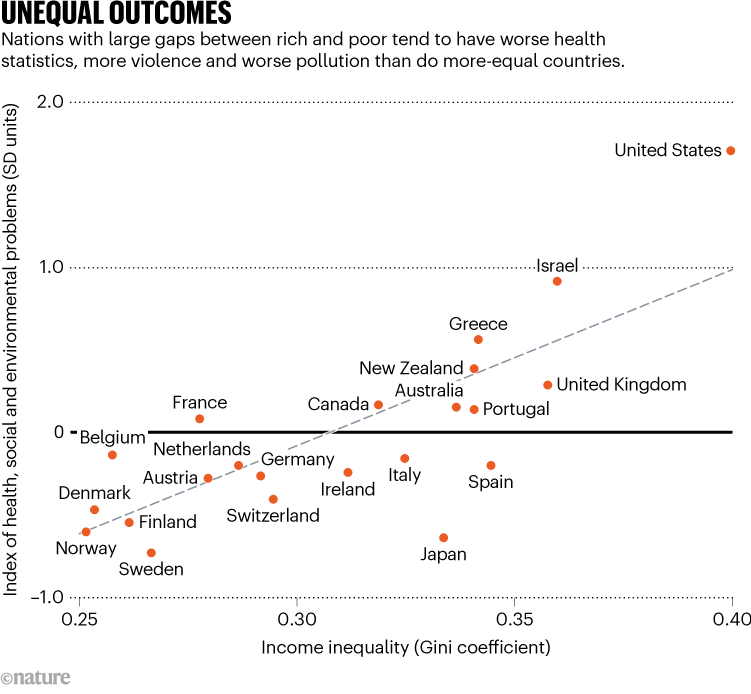
\includegraphics[keepaspectratio]{3_problem-analysis/images/fig11.png}}

}

\caption{\label{fig-unequal-outcomes}Income inequality and an index of
health, social, and environmental problems. Source: Wilkinson and
Pickett (2024).}

\end{figure}%

\subsection{Justice and inequality}\label{justice-and-inequality}

\emph{↗ Textbook chapter 6}

Questions about justice and just distribution concern almost every
social interaction in some way. While a ``sense'' of justice, much like
the capacity for language, is part of the basic mental equipment of
humans (although it can also be observed in non-human life), questions
of justice have been in focus since the beginnings of Western
philosophy. From Plato in ancient Greece to Martha Nussbaum in the 21st
century, very different conceptions of what makes a just society have
emerged. In what follows, we look at some approaches in more detail.

A good entry into the complex question of justice takes our intuitive
sense of justice as its starting point. This is often based on a form of
\textbf{reciprocity}, or mutuality. If I do you a big favour, we often
find it fair or just if you return the favour at some point, even if
possibly subject to our different dispositions. A first differentiation
is already hidden here: if we are on an equal footing or similarly
disposed, one speaks of ``balanced reciprocity'', but if our positions
differ fundamentally (for example rich/poor, king/subject), then justice
requires ``unbalanced reciprocity'', for example: whoever has more gives
more, but, depending on the case, also has more entitlement (Johnston
2011).

Although this reciprocity-based understanding of justice is still of
great importance in social psychology today, it played hardly any role
in the philosophy of justice for a long time -- even though it actually
stood at its very beginning. Plato formulates his definition of justice
as a direct answer to such an intuitive understanding, which is put
forward by Socrates' interlocutors (Plato's philosophy has been handed
down to us largely through so-called ``Socratic dialogues'', that is,
dialogues between Plato's teacher Socrates and other scholars). Plato's
approach, later developed further by his student Aristotle, no longer
defines justice through intuition but through a societal goal: what is
just is what serves the good life, which is why one speaks here of a
\textbf{teleological understanding of justice} (Greek \emph{telos} =
goal).

Although Plato and Aristotle do not clearly address many questions that
are significant today, the step towards a goal-oriented (or
consequentialist) concept of justice had major philosophical
consequences. A more modern variant of teleological justice,
\textbf{utilitarianism}, still represents an important philosophical
current today, one that is widespread among many neoclassical economists
in particular. At the core of utilitarianism is the search for the
greatest possible overall societal benefit (\emph{utility}), which is
achieved by calculating and maximizing the total sum of positive and
negative consequences. In utilitarian logic, it is therefore
permissible, for example, to treat equals unequally, as long as the
improvement (or utility gain) of one person is greater than the
deterioration (or negative utility) of another. What counts is the total
utility and thus also pure efficiency, or the maximum output that can be
achieved with a given quantity of resources -- regardless of its
distribution and even if the poor become poorer and the already rich
richer as a result. In this pure efficiency logic, however, the
radicalism of the utilitarian position is also hidden.

A closely related but weakened variant of utilitarian logic is a
definition of \textbf{justice as Pareto efficiency}. This maxim makes an
important exception: while it retains the goal of maximizing overall
societal utility, actions are accepted only if they make no one worse
off. A state that is more efficient in itself thus counts as
Pareto-superior only if no one is harmed at the same time. This
restriction is also significant because, unlike utilitarianism, it also
brings the well-being of the individual into focus: for us to define an
action as just, we no longer need information only about the total sum
of positive and negative utility but also about its distribution. This
opens the door to theories of justice that are no longer derived from a
societal goal but focus on the well-being of the individual and the
ethics of an action as such (so-called deontological theories). As we
saw in Chapter 2.5 (\emph{Abstract Markets or Capitalist Production
System}), this maxim forms the central reference point in neoclassical
economics for judging whether a (market) outcome is efficient. Since
this criterion can very rarely be met in reality, the Kaldor-Hicks
criterion is also frequently applied, which states that a change is
efficient for the economy as a whole if the winners could hypothetically
compensate the losers for their losses and would still be better off
afterwards. Whether the losers are then actually compensated for their
losses often plays no central role. With this criterion, we are back at
the utilitarian view.

Probably the most influential modern theory of justice was formulated in
1971 by the American philosopher \textbf{John Rawls}, drawing on his
deontological predecessors such as Immanuel Kant. Rawls addressed the
question of which rules the members of a society would agree on
regarding the distribution of resources without knowing their own
position, abilities, and conception of the good (Rawls 1999). Behind
such a ``veil of ignorance'', Rawls argues, people would, on the one
hand, agree on a system of equal basic liberties (such as respect for
human dignity) and, on the other hand, accept inequalities only under
two clear conditions:

\begin{quote}
``first, they are to be attached to offices and positions open to all
under conditions of fair equality of opportunity; and second, they are
to be to the greatest benefit of the least advantaged members of
society.'' (Rawls 1999)
\end{quote}

The first condition is widely known -- everyone should in principle get
the same opportunities. The second condition, the difference principle,
is less intuitive but also places well-founded limits on the equality of
outcomes. Since behind a veil we would not know our abilities either
(for example intelligence) -- and thus whether we would really have
equal opportunities in a world of pure equality of opportunity -- we
would accept inequalities only if they benefited the worst off the most.
If we assume, for example, that inequality boosts economic growth, then
this growth should benefit the poorest more than everyone else. A
well-known phrase in the preamble to the Swiss Federal Constitution
loosely takes up this thought: ``that the strength of the people is
measured by the well-being of its weakest members''. Rawls's \emph{A
Theory of Justice} subsequently became a kind of core reference to which
later theories of justice had to relate in order to distance themselves
from it and develop it further (Rawls 1999). Important contributions to
the debate criticized, on the one hand, the restriction of justice to
questions of distribution. Nancy Fraser and others emphasized in
particular the importance of fair processes, participation, and
recognition as a dimension of justice that precedes and is independent
of distribution (e.g. Fraser 1990).

On the other hand, the question gained in importance of what should
actually be distributed justly -- and, in subtle allusion to the ancient
Greeks, what this has to do with the good life. Especially since the
1980s and 1990s, thinkers have engaged in various ways with the
observation that human development and a life worth living can be
measured only to a limited extent by material prosperity. Two of the
most important voices in this debate are the economist and philosopher
Amartya Sen and the philosopher Martha Nussbaum, whose work underlies
the now widespread Human Development Index (HDI) (see Chapter 2.1.2,
\emph{Alternative indicators of prosperity}). Besides material
prosperity, this index also captures life expectancy and the number of
years of schooling, but it is based on Sen's and Nussbaum's concept of
so-called ``capabilities'' (Nussbaum 2003; Sen 1999). Instead of a
universal measure of development (such as material prosperity or
resources), the capabilities approach puts people's own ideas of
well-being at the centre, or rather each person's capabilities to
realize these ideas. Since the resources required for this can differ
greatly depending on the person and context, the focus on capabilities
embodies a significant departure from concepts of justice and of the
good life that rest exclusively on material prosperity. By moving
non-material dimensions of well-being to the centre, such as the
possibility of maintaining personal relationships or leading a long and
satisfying life, the capabilities approach presents a slightly
relativizing view of the dominance of economic realities and
inequalities for human well-being.

As the
\href{https://hdr.undp.org/content/human-development-report-2025}{Human
Development Report} published by the United Nations regularly shows,
however, the HDI, too, is led by the materially richest countries.
Regardless of which concept of prosperity and justice we use, it is
therefore worth taking a closer look at the origins of economic
inequality.

\subsection{Types and causes of
inequality}\label{types-and-causes-of-inequality}

\emph{↗ Textbook chapter 17}

Inequalities in material prosperity, but also in the form of
capabilities, have, on the one hand, grown historically, with global
inequality in particular still being fundamentally shaped by colonial
and postcolonial relations of domination. At the same time, these
historically grown inequalities can also be observed ``on a small
scale'': those who grow up with rich parents have a significantly higher
chance of themselves being prosperous one day: access to education,
hobbies, resources, networks, and so on explain a large part of
intergenerational income inequality (Corak 2013). With regard to wealth
inequality, the factor of inheritance also comes into play: those who
start life with substantial assets usually not only keep them but can
often count on equally substantial passive income (for example from
renting out residential buildings) or on independent appreciation in
value (for example if the residential buildings were built long ago in a
location that is central today and could be sold for many times the
price).

At the same time, every ``historical'' inequality is also to be
understood as the result of current economic and political conditions.
Whether wages, profits, inheritance, redistribution, or even
expropriation are perceived as just ultimately depends on the prevailing
ideas of justice and how these manifest themselves politically. Besides
taxes and welfare-state questions, this concerns in particular various
areas of economic policy and the underlying economic paradigms. But what
do the questions about distribution and inequality refer to concretely?
In economics, several important distinctions are made in the first
place: between income and wealth, between primary and secondary
distribution, and between national and global inequality:

\begin{itemize}
\item
  \textbf{Income and wealth}: The total product of an economy (as
  measured by GDP) can also be understood as the summed income of the
  factors of production, that is, wages for labour, ground rent or rent
  for land, and profits and interest on capital. The shares that these
  factors of production earn of total income, or how income is
  distributed within these groups, is called income distribution, and
  its unequal distribution is called income inequality. Distribution and
  inequality of wealth, in turn, refer to the already ``distributed''
  ownership of accumulated property, understood as a result rather than
  a process, in the form of money or possession of land (such as a
  single-family house or agricultural land) and capital (such as
  tractors or company shares). Wealth stands in a twofold relationship
  to income: on the one hand, a person's wealth corresponds to the
  accumulation of their personal income, although inheritance,
  especially among very wealthy people, is usually at the origin of
  their riches. On the other hand, wealth opens up new sources of income
  when it is invested in capital or land. The phrase ``letting your
  money work for you'' refers to precisely this connection.
\item
  \textbf{Primary and secondary distribution}: This concerns income
  exclusively: primary distribution refers to the direct distribution of
  total income to the factors of production (or to workers and owners of
  capital and land). Secondary distribution refers to the outcome of
  distribution after state intervention, in particular through
  redistribution via taxes, which is meant to correct an overly unequal
  primary distribution (for example by supporting the unemployed with
  state funds, financed by taxing everyone else). The division into
  primary and secondary distribution is intuitive but contested, since
  it hides the role of the state in primary distribution and presents
  the latter as a quasi natural market outcome. Instead of primary and
  secondary distribution, people therefore also speak of functional and
  personal distribution (see textbook chapter 17).
\item
  \textbf{National and global inequality}: When inequality is talked
  about, it is often either about the unequal distribution of income or
  wealth within a country, but just as often about inequality between
  countries. This distinction is indispensable for a meaningful
  discussion and can lead to a lot of confusion. For example, we
  generally have an approximate understanding of poverty in countries of
  the Global South, but struggle to compare the life of a rich person
  there with that of a poor person living in Switzerland.
\end{itemize}

In what follows, we first turn to income inequality and in particular to
primary distribution in order to explore the causes of inequality from
an economic perspective, but we already do so with an eye to both
national and international distribution.

\subsection{Division of labour and comparative
advantage}\label{division-of-labour-and-comparative-advantage}

Besides the invisible hand, Adam Smith's pin factory is probably the
best-known excerpt from his work. The first chapter deals with the
division of labour in a pin factory and how it raises productivity to a
great extent. Deriving from this, Adam Smith states more generally how
productivity rises through the division of labour. Individuals,
companies, or countries that specialize in an activity can perform it
increasingly well. This creates an absolute advantage in production over
others. Economic subjects increasingly specialize in those areas in
which they are better than others. If a subject is superior to another
in no area, it cannot take part in trade.

David Ricardo later criticizes Smith's theory of absolute advantages. If
one economic subject were superior to another in all respects, then,
according to Smith, it would also produce everything itself. Ricardo, by
contrast, establishes the theory of comparative advantage. It states
that subjects produce those goods for which they have the greatest
\emph{comparative advantage}, or the smallest relative disadvantage,
over others. Here it still makes sense for subjects that are superior to
others in no activity to participate in a shared economy. In doing so,
they take on tasks for which others are better qualified but which those
others do not prioritize because of a lack of resources.

Ricardo worked out his theory using the example of trade (cloth and
wine) between England and Portugal and wanted to show in this way that
free trade would be worthwhile for both sides. It was a plea against the
then omnipresent import restrictions and tariffs between countries,
which were based on mercantilist logic. This short
\href{https://www.srf.ch/play/tv/eco/video/komparativer-kostenvorteil?urn=urn:srf:video:ff4bef24-b498-42cc-8d98-25353e7a1f71}{video}
(in German) illustrates the basic idea behind Ricardo's theory of
comparative cost advantages.

Ricardo is thus often drawn upon to illustrate that free trade is
advantageous for all countries involved. This perspective, which is very
widespread in neoclassical economics, should certainly be viewed
critically, as many other schools of thought emphasize. For one thing,
the notion of ``free'' trade quickly becomes relative in the context of
European imperialism, which was emerging at the time when Ricardo
developed his theory. In this period, the global market was shaped under
the prevailing power relations primarily to the advantage of the Global
North, was based on the exploitation of the Global South, and created
unequal structures that in part persist to this day (see, for example,
Anievas and Nişancıoğlu 2015; Davis 2017; Ghosh 2021; Hickel 2017;
Patnaik and Patnaik 2021). In addition, advantageous participation in
global trade requires a country to have competitive industries. Western
Europe and the USA, too, built up their industries under the protection
of the global market and with state industrial policy (Chang 2002). The
forced further economic opening of many countries in the Global South
from the end of the 1970s onwards by institutions such as the
International Monetary Fund, for example, made it harder to develop
their own competitive manufacturing industries and pushed these
countries back into the production and extraction of raw materials (see,
e.g., Chang and Palma 2003). Dorninger et al. (2021) show how strongly
this unequal exchange manifests and materializes in various aspects (for
example land use and resource consumption) (see
\textbf{?@fig-resourceuse}).

\subsection{Power relations, labour share, and wealth
inequality}\label{power-relations-labour-share-and-wealth-inequality}

The countries that benefited in this way from their industrial head
start, while drawing on everyone else, also had to ensure at the
national level that inequality stayed within (social) limits. In the
middle of the 20th century, the American economist Simon Kuznets even
put forward the hypothesis that in states with increasing economic
growth, income inequality would first increase but would decrease again
beyond a certain level. The so-called ``Kuznets curve'' arose in a time
of flourishing social market economies in the 1950s and 1960s, when in
the growing economies of the Global North \textbf{profits were broadly
distributed to workers and the highest incomes were taxed strongly
progressively}.

\begin{figure}[H]

{\centering \pandocbounded{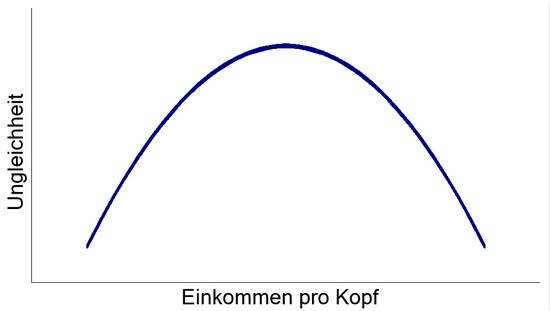
\includegraphics[keepaspectratio]{3_problem-analysis/images/fig12.png}}

}

\caption{Kuznets curve. Source: Own illustration.}

\end{figure}%

\begin{tcolorbox}[enhanced jigsaw, arc=.35mm, bottomrule=.15mm, bottomtitle=1mm, breakable, colback=white, colbacktitle=quarto-callout-tip-color!10!white, colframe=quarto-callout-tip-color-frame, coltitle=black, left=2mm, leftrule=.75mm, opacityback=0, opacitybacktitle=0.6, rightrule=.15mm, title={Excursus: The idea of the Kuznets curve persists stubbornly}, titlerule=0mm, toprule=.15mm, toptitle=1mm]

Inequality in income and wealth -- a question of belief?

In the following \href{https://ilias.unibe.ch/go/xvid/3803471}{podcast}
(in German) by Swiss Radio and Television SRF, Graeme Maxton, economist
and former Secretary General of the Club of Rome, and Samuel Rutz,
economist and head of department at Avenir Suisse, discussed the extent
and causes of inequality.

\end{tcolorbox}

With the emergence of neoliberal reforms from the 1980s onwards, an
increasing polarization of incomes became apparent strongly in the USA,
but to a weaker degree also in Europe. Since then, the share of the
richest 10\% in total income has risen, while that of the bottom 50\%
has increasingly declined (see, for example, the
\href{https://wid.world/}{World Inequality Database}). Rather than a
kind of law of nature, the causes of inequality are ultimately an
interplay of existing economic conditions and political framework
conditions. An important cause of rising income inequality is
\textbf{the changing power relations between labour and capital in an
opening world economy}. While a large part of financial capital can now
travel around the world in fractions of a second at the click of a
mouse, the mobility of employees has risen only comparatively little.
Both institutional factors such as borders and social motives such as
families or friendships slow down the factor of production labour. The
compromise previously established between companies and employees
organized in trade unions came under pressure in many places. As a
consequence, the labour share, that is, the share of earned income in
total economic output, is falling today in many countries, while the
share of capital income is rising. While up to the 1970s clearly more
than half of GDP was earned through labour, this share fell below the
50\% mark in most countries in the 2000s. Besides economic
globalization, this trend is also strongly shaped by technological
development. In view of the rapid acceleration, in particular through
the widespread application of artificial intelligence, no quick reversal
of the trend is in sight (Dao et al. 2017). It is much more likely that
income differences due to the division of labour will, over time,
increasingly be overshadowed by differences between labour and capital
income.

This in turn fuels the equally fast-growing \textbf{wealth inequality}.
For however great the inequality of incomes is, it is overshadowed by
the inequality of wealth -- that is, the total of all goods a person is
entitled to. In 2013, with his work \emph{Capital in the Twenty-First
Century}, the French economist Thomas Piketty showed how wealth
inequality has historically grown again since the middle of the 20th
century (Piketty and Goldhammer 2014). As the main driver behind this,
he sees that capital incomes have grown faster than the real economy.
The consequence is that rich people, who can invest in capital goods,
gain access to wealth growth that remains closed to working people.
Waves of political liberalization after the neoliberal turn of the 1980s
also favour the increase in wealth inequality. Through low inheritance
taxes or the privatization of state-owned companies, for example, wealth
becomes concentrated among a few rich persons. The trend towards
increased wealth inequality is reflected each year in even more extreme
figures: as early as 2016, an Oxfam study (based on Credit Suisse data)
noted that the richest one per cent held as much wealth as the rest of
humanity combined -- and that only 62 people owned as much as the poorer
half of the world's population. In 2025, it took only 12 (Maitland et
al. 2026).

\subsection{National and global
inequality}\label{national-and-global-inequality}

\emph{↗ Textbook chapter 20}

\begin{figure}[H]

\centering{

\pandocbounded{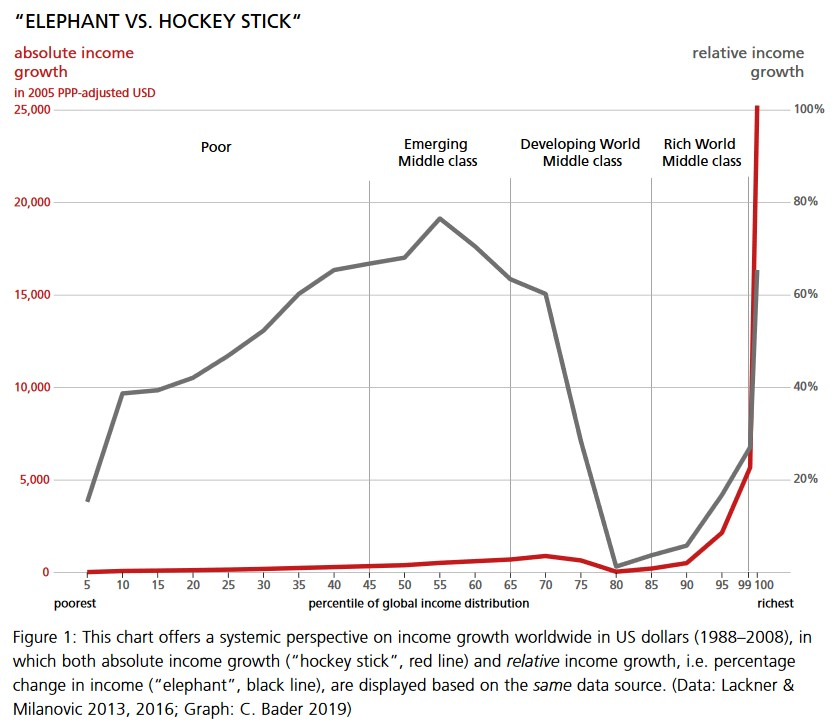
\includegraphics[keepaspectratio]{3_problem-analysis/images/fig13.png}}

}

\caption{\label{fig-elephant-hockey}Elephant or hockey stick? Source:
Lannen et al. (2019).}

\end{figure}%

At the global level, between 1988 and 2008, a picture emerges that is
similar to that in high-income countries. The curve of \textbf{relative
income growth (Figure~\ref{fig-elephant-hockey} in black)} does show
that incomes in the middle percentiles of global incomes have grown
relatively strongly. This represents the rapid emergence of
middle-income groups in countries such as China or Brazil. The lowest
quantiles make clear how incomes in Africa and South Asia are growing
only slowly. The trough between the richest 80 and 95 per cent depicts
large parts of North America and Europe, where middle incomes have
stagnated since the neoliberal reforms mentioned above. This depiction,
known as ``Milanovic's elephant'', thus contains information on several
phenomena at once. When looking at the \textbf{absolute income growth
(Figure~\ref{fig-elephant-hockey} in red)} -- also referred to as the
``hockey stick'' -- it becomes clear, however, how strongly the incomes
of the richest people grew in this period (Green 2016). More than half
of all income gains in this period went to the richest five per cent of
the world's population. The poorer half of the world's population
received only one tenth of the income.

While the globalization of the economy in recent decades (as well as the
first globalization 150 years ago) is thus often portrayed in a positive
light, and it is shown how free international trade leads to global
prosperity, it also reveals new social limits. As the economist Branko
Milanovic described more than 20 years ago, this \textbf{second face of
globalization}, a face of exploitation and destruction (or colonialism),
is overlooked (Milanovic 2003). Globalization is a phenomenon of
enormous size and complexity and can accordingly show both its beautiful
and its cruel face at the same time (depending on to whom the face
reveals itself) (Milanovic 2003). Besides the fact that global
capitalism has led to great growth in material prosperity in many
places, an increase in inequality could also be observed, as explained
above. Moreover, the economic system was based in many places on
colonial and imperial violence. The structures still lead in many places
to exploitation, dependencies, and unequal exchange (see, for example,
Anievas and Nişancıoğlu 2015; Davis 2017; Ghosh 2021; Hickel 2017;
Patnaik and Patnaik 2021).

Dorninger et al. (2021) show that high-income countries claim more
resources, land, energy, and labour than they produce themselves. There
is thus an \textbf{unequal exchange between the different groups of
countries}. In addition, the globalized world economy and the
corresponding institutions push many countries in the Global South into
the production of raw materials (see, for example, Chang and Palma
2003). At the same time, many countries engage in more highly
specialized industry and services, where more value can be captured.
Global value chains are often controlled by companies in the Global
North, which reinforces this unequal exchange and enables these
companies to capture the bulk of the profit and shift the costs to the
Global South (see, for example, Althouse et al. 2023; Durand and Milberg
2020; Ponte 2022). Such constellations increase the pressure on working
conditions and favour exploitative relations in the Global South.

This is only a small and simplified excerpt from the complexity of the
globalized economy. Many aspects are still insufficiently researched and
in part contested. The point here is above all to show that, as
Milanovic (2003) argues, globalization has at least two faces. Which one
it shows has to be examined in each individual case.

\chapter{Strategies for a Sustainable Economy: Efficiency, Consistency,
Sufficiency}\label{strategies-for-a-sustainable-economy-efficiency-consistency-sufficiency}

\begin{tcolorbox}[enhanced jigsaw, arc=.35mm, bottomrule=.15mm, bottomtitle=1mm, breakable, colback=white, colbacktitle=quarto-callout-note-color!10!white, colframe=quarto-callout-note-color-frame, coltitle=black, left=2mm, leftrule=.75mm, opacityback=0, opacitybacktitle=0.6, rightrule=.15mm, title={Guiding question}, titlerule=0mm, toprule=.15mm, toptitle=1mm]

In Chapter 3, we saw why our economy fails to achieve its goal --
prosperity for all, within ecological limits. What fundamental levers
are there to change this?

\end{tcolorbox}

In view of the ecological limits of our planet, most highly
industrialized countries share a broad scientific and political
consensus that ecological limits (planetary boundaries) should be
respected in the long term. The 1.5-degree and 2-degree targets, a
central climate policy goal, have also been enshrined internationally in
the \href{https://www.fedlex.admin.ch/eli/fga/2017/81/en}{Paris
Agreement}, which Switzerland has signed. With regard to economic and
social limits, too, the global community has committed itself through
the \href{https://sdgs.un.org/2030agenda}{2030 Agenda}, and Switzerland
specifically through the goals of the
\href{https://www.are.admin.ch/are/en/home/sustainable-development/strategy/sds.html}{Sustainable
Development Strategy 2030}. These goals require a fundamental
transformation of how we do business within a few decades.

This raises the decisive question: \emph{how} exactly should this
transformation succeed? The sustainability debate discusses three
fundamental strategies: \textbf{efficiency}, \textbf{consistency}, and
\textbf{sufficiency}. Practically all approaches to sustainable
development build on these three strategies, but they differ in how they
weigh their interplay and prioritization. Ultimately, achieving the
sustainability goals probably requires all three working together:

\begin{figure}[H]

{\centering \pandocbounded{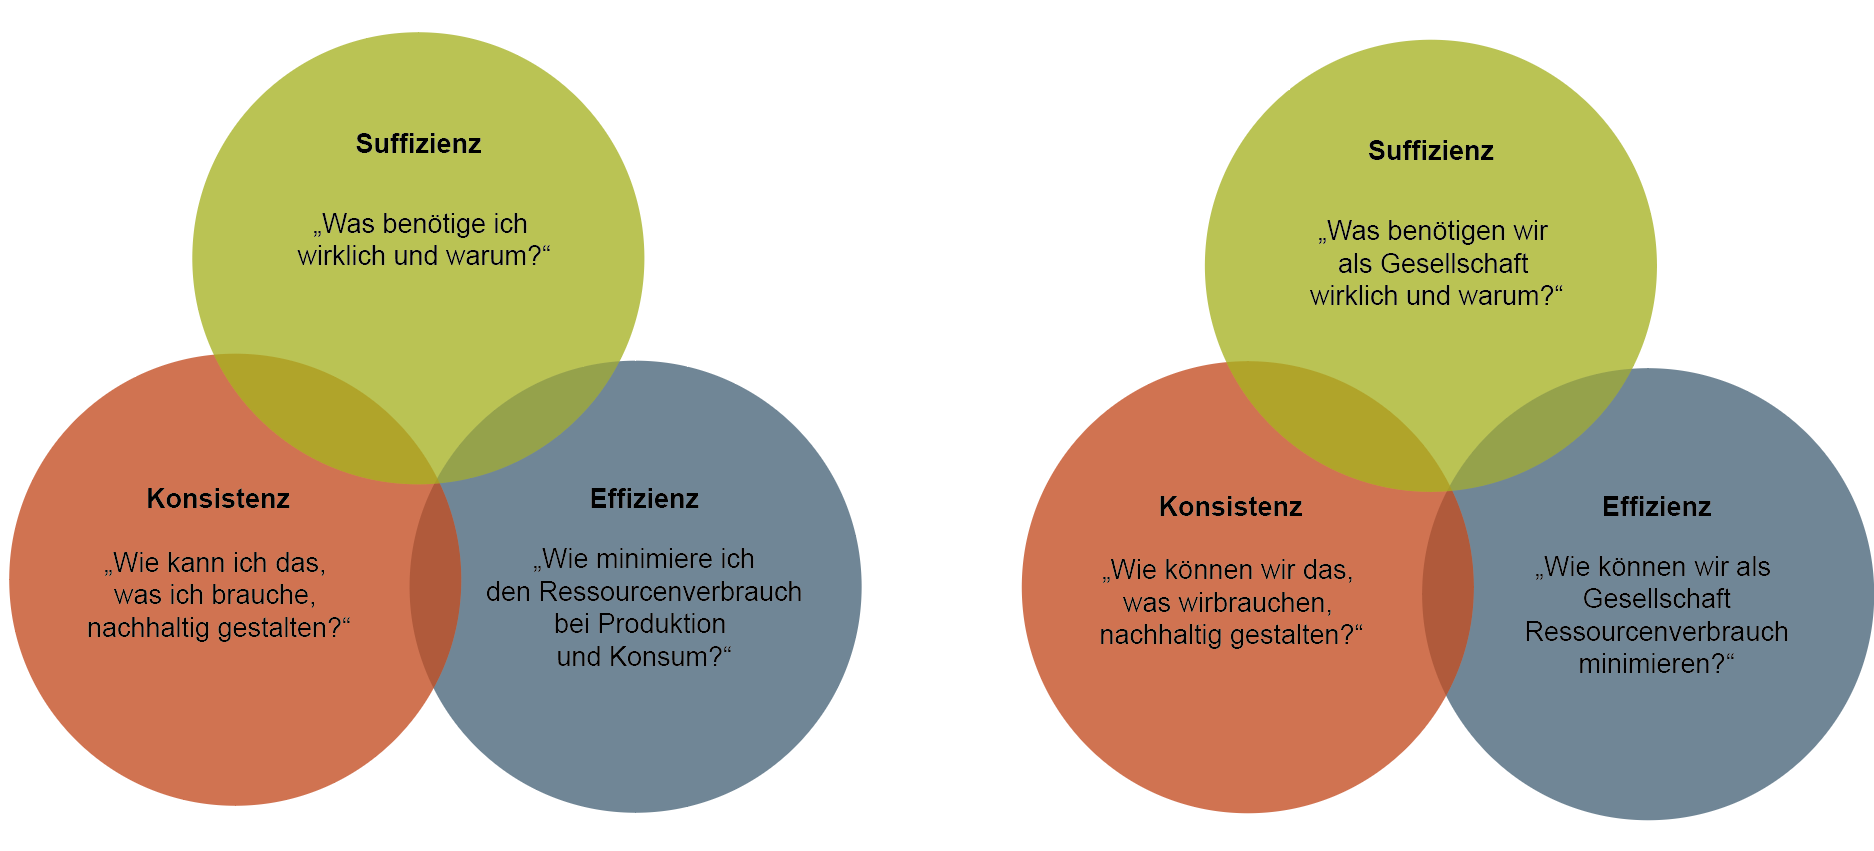
\includegraphics[keepaspectratio]{4_strategies/images/fig1.png}}

}

\caption{The three sustainability strategies. Source: Own illustration.}

\end{figure}%

\section{Efficiency Strategy}\label{efficiency-strategy}

The efficiency strategy aims to use fewer resources (raw materials and
energy) than before when manufacturing products or providing services,
without reducing the quantity produced. This includes minimizing
material consumption (material intensity), energy consumption (energy
intensity), and the emission of harmful substances such as
CO\textsubscript{2}. This concept is often called
\textbf{eco-efficiency}. Business and society regard it as promising
because it can reduce costs, resource consumption, and environmental
impacts. The efficiency strategy starts on the production side, where
change is sought primarily through technological progress. Proponents of
this approach believe it is possible to double prosperity while halving
the use of nature (Weizsäcker et al. 1997). Critics of the efficiency
strategy are less optimistic, however, and warn against overestimating
its effects on sustainable economic activity. They point to so-called
\emph{rebound effects} (see Chapter 3.1.3, \emph{Climate crisis --
market failure or systemic problem}), which can cause the gains from
efficiency improvements to be smaller or even cancelled out (Paech 2012;
Santarius 2014).

\begin{tcolorbox}[enhanced jigsaw, arc=.35mm, bottomrule=.15mm, bottomtitle=1mm, breakable, colback=white, colbacktitle=quarto-callout-tip-color!10!white, colframe=quarto-callout-tip-color-frame, coltitle=black, left=2mm, leftrule=.75mm, opacityback=0, opacitybacktitle=0.6, rightrule=.15mm, title={Examples of the efficiency strategy}, titlerule=0mm, toprule=.15mm, toptitle=1mm]

\begin{itemize}
\tightlist
\item
  \textbf{Energy-efficient lighting}: Replacing conventional
  incandescent bulbs with energy-efficient LED lamps reduces electricity
  consumption and helps to lower energy demand.
\item
  \textbf{Fuel-efficient vehicles}: Developing hybrid or electric
  vehicles with improved fuel consumption reduces fuel demand and
  road-traffic emissions.
\item
  \textbf{Efficient building technology}: Installing smart heating,
  ventilation, and air-conditioning systems in buildings helps to reduce
  the energy used for heating and cooling.
\item
  \textbf{Efficient water use}: Using water-saving fittings and systems
  in households and industrial companies reduces water consumption and
  minimizes waste.
\end{itemize}

\end{tcolorbox}

\section{Consistency Strategy}\label{consistency-strategy}

The efficiency strategy is quantity-oriented -- less resource use for
more output. By contrast, the consistency strategy seeks compatibility
between nature and technology, aiming to use resources repeatedly rather
than consuming them only once. This implies replacing materials,
products, and technologies that often rely on fossil resources with ones
that match natural material cycles and operate in harmony with natural
processes (Pufé 2017). This is often called \textbf{eco-effectiveness}
and follows the ``cradle to cradle'' principle, in which products go
from ``cradle to cradle'' instead of from ``cradle to grave''. The idea
behind it is that in intelligent systems there is no waste, only
products. This can happen in two ways: materials can either be
biodegradable, as with shampoo free of synthetic ingredients, or they
can be designed as ``technical nutrients'' that remain in the technical
cycle. This means that a product at the end of its life does not end up
in the bin but passes into a next cycle of use, for example by being
upcycled. A computer casing, for instance, could be reused again and
again or converted into a shelving system. The consistency strategy,
too, starts on the production side. It is expected to offer great
problem-solving potential, a wider reach, and more profound change than
the efficiency strategy.

\begin{figure}[H]

{\centering \pandocbounded{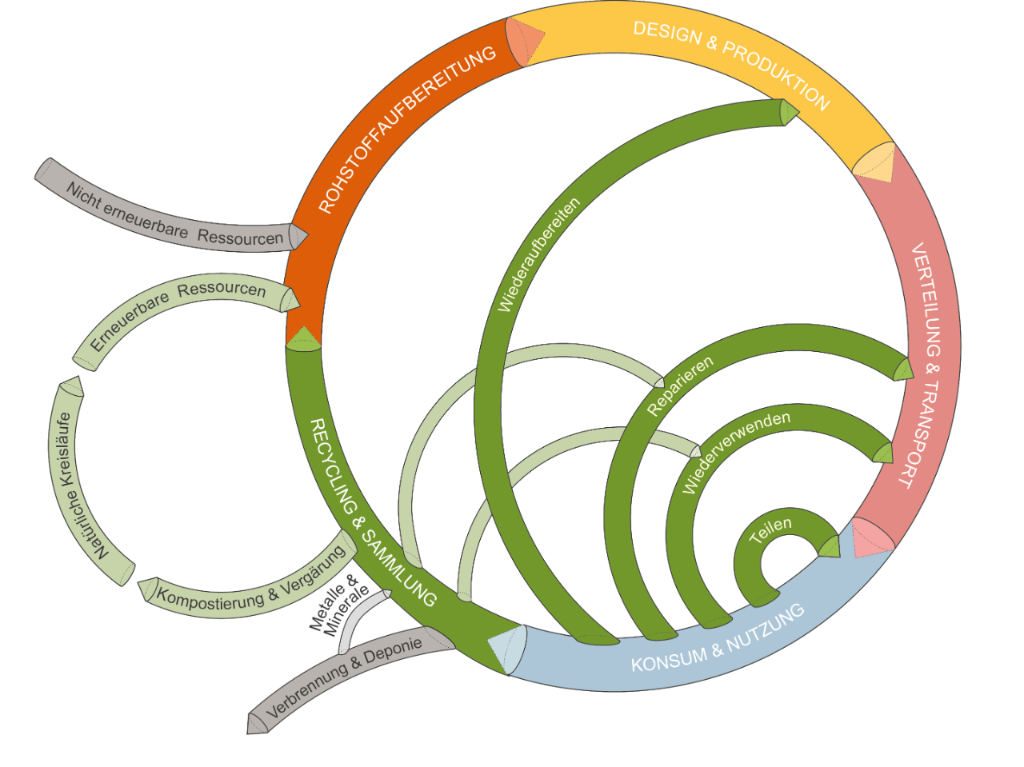
\includegraphics[keepaspectratio]{4_strategies/images/fig2.png}}

}

\caption{Schematic illustration of the circular economy. Source: BAFU
(2019).}

\end{figure}%

Nevertheless, the economy's material cycles cannot be achieved without
losses of mass and energy, so absolute consistency remains an
unattainable ideal. Even products that are 100\% biodegradable consume
energy in their production. Consistency is nonetheless understood as an
impetus for industry to strive for this ideal and to reduce both
resource consumption and emissions as far as possible.

\begin{tcolorbox}[enhanced jigsaw, arc=.35mm, bottomrule=.15mm, bottomtitle=1mm, breakable, colback=white, colbacktitle=quarto-callout-tip-color!10!white, colframe=quarto-callout-tip-color-frame, coltitle=black, left=2mm, leftrule=.75mm, opacityback=0, opacitybacktitle=0.6, rightrule=.15mm, title={Examples of the consistency strategy}, titlerule=0mm, toprule=.15mm, toptitle=1mm]

\begin{itemize}
\tightlist
\item
  \textbf{Renewable energy systems}: The transition from fossil fuels to
  renewable energy sources such as solar, wind, and hydropower ensures
  that energy is produced in harmony with the natural rhythms and cycles
  of the environment.
\item
  \textbf{Electronics designed for circularity}: Electronic devices are
  designed so that they can be easily repaired, upgraded, and recycled,
  in order to minimize resource consumption and environmental impact.
\item
  \textbf{Sustainable construction}: Buildings are constructed using
  sustainable materials that have low environmental impacts and can be
  reused or recycled at the end of their service life.
\end{itemize}

\end{tcolorbox}

\section{Sufficiency Strategy}\label{sufficiency-strategy}

Sufficiency questions the level of need for a good life and aims to
reduce resource and energy consumption through lower demand for
resource-intensive goods and services. It is often also translated as
moderation or appropriateness. Sufficiency takes a critical view of the
new needs created by technology and advertising in relation to limited
natural resources. It fosters an understanding that we need not ``chase
after'' every newly created need, and that needs can be satisfied
without consumption. Unlike efficiency and consistency, sufficiency
focuses on the consumption side, though not exclusively. It can be
practised to different degrees and at different levels, from smaller
changes in behaviour (sharing rather than buying) to substantial changes
in how we live (giving up air travel). Although it begins at the
individual level, sufficiency can be applied at various levels,
including companies (sufficiency-oriented product design) and
governments (sufficiency policy). Sufficiency thus asks what the right
measure is: How much do we need for a good life? And what do we not
need? The sufficiency strategy is the subject of a passionate and
intensive debate (Sedlacek 2012).

Critics consider the sufficiency strategy limited in its savings
potential and its sociocultural resonance. They doubt that it can find
broad acceptance. By contrast, proponents argue that the sufficiency
strategy occupies an essential place in sustainability policy,
especially where the efficiency and consistency strategies reach their
limits.

\begin{tcolorbox}[enhanced jigsaw, arc=.35mm, bottomrule=.15mm, bottomtitle=1mm, breakable, colback=white, colbacktitle=quarto-callout-tip-color!10!white, colframe=quarto-callout-tip-color-frame, coltitle=black, left=2mm, leftrule=.75mm, opacityback=0, opacitybacktitle=0.6, rightrule=.15mm, title={Examples of the sufficiency strategy}, titlerule=0mm, toprule=.15mm, toptitle=1mm]

\begin{itemize}
\tightlist
\item
  \textbf{Sharing and communal use}: Platforms and initiatives for
  sharing objects, tools, or vehicles make it possible to use resources
  more efficiently and to reduce the number of products manufactured.
\item
  \textbf{Plant-based diets}: Switching to a mainly plant-based diet
  reduces the demand for resources such as water and land compared with
  meat production.
\item
  \textbf{Working-time reduction}: Reducing working time can lead to
  lower resource consumption, since less energy and fewer materials are
  needed to produce goods and services.
\item
  \textbf{Local consumption}: Supporting local producers and markets
  helps to reduce transport distances and emissions.
\end{itemize}

\end{tcolorbox}

\begin{tcolorbox}[enhanced jigsaw, arc=.35mm, bottomrule=.15mm, bottomtitle=1mm, breakable, colback=white, colbacktitle=quarto-callout-caution-color!10!white, colframe=quarto-callout-caution-color-frame, coltitle=black, left=2mm, leftrule=.75mm, opacityback=0, opacitybacktitle=0.6, rightrule=.15mm, title={Further reading}, titlerule=0mm, toprule=.15mm, toptitle=1mm]

To explore the sufficiency strategy in more depth, read the Denknetz
article \href{https://ilias.unibe.ch/go/file/3803485}{``The New Debate
on Sufficiency''} (in German).

\end{tcolorbox}

\chapter{The Role of the State and Economic Policy Guiding
Models}\label{the-role-of-the-state-and-economic-policy-guiding-models}

\emph{↗ Textbook chapters 10 and 21}

\begin{tcolorbox}[enhanced jigsaw, arc=.35mm, bottomrule=.15mm, bottomtitle=1mm, breakable, colback=white, colbacktitle=quarto-callout-note-color!10!white, colframe=quarto-callout-note-color-frame, coltitle=black, left=2mm, leftrule=.75mm, opacityback=0, opacitybacktitle=0.6, rightrule=.15mm, title={Guiding question}, titlerule=0mm, toprule=.15mm, toptitle=1mm]

How can a society ensure that its economy actually achieves the goal we
took as our starting point in Chapter 2 -- prosperity for all, within
ecological limits?

\end{tcolorbox}

We have covered a lot of ground in this script. In Chapter 1, we saw
that there is no single economics, but rather different schools of
thought, each with its own basic assumptions. In Chapter 2, we examined
prosperity as the actual goal of economic activity. We asked what is
used to provide this prosperity (factors of production, goods) and how
this provision is coordinated. In Chapter 3, we saw that today's economy
misses this goal in several respects, and in Chapter 4, we encountered
three strategies for addressing these problems: efficiency, consistency,
and sufficiency. This closes the circle with the original question from
Chapter 2: How must an economy be coordinated so that prosperity for
all, within ecological limits, is actually achieved?

This brings us to the question of implementation: Who actually ensures
that we get there? The market alone, or do we need the state? This
question cannot be answered independently of what we have already seen.
Depending on one's understanding of the economy, markets, and
capitalism, the answer on the role of the state differs as well -- from
an intervention limited to market failure to a state that actively
shapes the economy or even sets limits.

These different ideas about the state and the market do not simply stand
side by side in isolation. In practice, they condense into larger,
coherent \textbf{economic policy guiding models} -- that is, overall
pictures of how the state, the market, and society should interact in
order to achieve the shared goal. In this course, following Novy et al.
(2023), we distinguish three basic economic policy guiding models that
can be observed today as the result of the influence of different
schools of thought: \textbf{market liberalism}, \textbf{welfare
capitalism}, and \textbf{post-growth}. Each of them can be traced back
to the styles of thought that accompany us throughout the script.

\section{Why ``Market vs.~State'' Is Historically Not a
Given}\label{why-market-vs.-state-is-historically-not-a-given}

\begin{figure}[H]

{\centering \pandocbounded{
\includegraphics[keepaspectratio]{5_state-and-guiding-models/images/fig1.png}}

}

\caption{SRF report, 15 March 2023. Source:
\url{https://www.srf.ch/news/schweiz/wohnungen-werden-knapper-staatliche-wohnbaufoerderung-oder-mehr-freier-markt}.}

\end{figure}%

That we can speak at all of the state ``intervening in the market'' is
not a universal historical truth. For people who lived before the
emergence of modern capitalism, this formulation would simply have made
no sense. In this chapter, we explore the specific role of the state in
capitalism and how the actions of state institutions in relation to the
economy can be explained.

As we saw in the introductory chapter, it was only with the transition
from feudalism to industrial capitalism that the economy came to be
thought of as a supposedly separate sphere, detached from political
power. Ellen Meiksins Wood (2017) shows that under feudalism, economic
and political rule were inseparably linked: the nobility appropriated
part of the serfs' production through direct political coercion. Wage
labour was a marginal phenomenon at the time, and production was shaped
by craft workshops, agriculture, and subsistence production. In the
transition to industrial capitalism and emerging liberalism, the state
came to be understood as the sphere of power, of its distribution and
limitation, and increasingly of democratic participation. In contrast
stood civil society, which was understood as a part of society separate
from the state, protected by rights, and characterized by the
individual, rational pursuit of economic interests. The economy was thus
conceived, in particular through the right to private property, as a
separate space protected from the state and understood as largely free
of power relations.

When we talk today about the right form of the state, we usually mean
the liberal parliamentary democracy, in which elections take place but
which also protects private property from state interference. The
economy is thus not an area in which democratic procedures have a place.
When we go to the supermarket, we do not face goods that we have agreed
on as a society, but goods that the supermarket chain considers
profitable. When we go to work, we do not expect to have a say in
production goals and the distribution of profits, but accept our
employer's decisions in return for a wage. Democracy thus takes place in
the political sphere through elections, but in everyday life, which is
shaped above all by wage labour and the purchase of goods, the
possibility of exerting democratic influence on our living conditions is
limited (Anderson 2019).

That we can meaningfully speak of ``state interventions in the market''
today is therefore itself the product of a specific historical and
political constellation, and hence not a neutral starting point. This
insight is central to the following sections: if the separation between
market and state is historically made, then the question of \emph{how}
the state and the market should relate to each other is not a purely
technical one but always also a political one.

\section{Market-Liberal Guiding Model: The State as
Night-Watchman}\label{market-liberal-guiding-model-the-state-as-night-watchman}

In the most widely used economics textbook (Mankiw and Taylor 2020), the
role of the state is defined through four concepts: property rights,
market power, market failure, and externalities. The market is
considered fundamentally efficient, and deviations require
justification. This gives rise to a certain circular reasoning, however:
if the market leads to poor outcomes, the market itself is never at
fault, but rather incomplete property rights or incomplete markets.
Accordingly, new markets must be created instead of questioning the
market as an organizing principle. This very circular reasoning is the
starting point for Samuel Bowles's critique (see below).

David Harvey summarizes the prevailing basic idea of the role of the
state from a neoclassical perspective as follows:

\begin{quote}
``State interventions in markets (once they have been created) must be
kept to an absolute minimum, because according to the theory the state
cannot possibly have enough information to anticipate market signals
(prices)'' (translated from Harvey 2005, 3)
\end{quote}

Today, this understanding is often referred to by the term
\emph{night-watchman state}. In contrast, critics such as Michel
Foucault and Quinn Slobodian point out that enforcing, maintaining, and
managing markets by no means results in a weak state but requires a
strong one (Slobodian 2018).

We call the role of the state described here on the basis of a
neoclassical understanding -- limited to guaranteeing private ownership
of the means of production (property rights), preventing monopolies
(market power), and limited interventions to correct market outcomes
(market failure and externalities) -- the \textbf{market-liberal guiding
model}.

\subsection{Critique of the market-liberal guiding model: markets are
not neutral -- they
constitute}\label{critique-of-the-market-liberal-guiding-model-markets-are-not-neutral-they-constitute}

An important critique of the market-liberal guiding model and the role
it assigns to the state arises from the observation that its concept of
market failure is often too narrow. The economist Samuel Bowles, for
instance, argues that markets not only allocate resources and distribute
income but also \textbf{shape culture, preferences, and power
structures}. They are thus ``as much political and cultural institutions
as economic ones'' (Herzog et al. 2014, 471). Four building blocks
support this argument:

\begin{itemize}
\tightlist
\item
  \textbf{Endogenous vs.~exogenous participants.} The abstract textbook
  market, as we discussed it in Chapter 2.5, assumes exogenous,
  unchanging preferences. Once participants are \emph{endogenous} (the
  market itself affects their abilities, values, and wishes), allocation
  in markets no longer works as efficiently as described in the model,
  because the model relies on precisely this exogeneity assumption
  (Herzog et al. 2014, 481).
\item
  \textbf{Contested markets.} Where claims are enforced endogenously (by
  the participants themselves rather than by third parties), a power
  relationship arises between the side facing greater scarcity and the
  other side, ``even if the exchange takes place under full information,
  without coercion, and under fully competitive conditions'' (Herzog et
  al. 2014, 478).
\item
  \textbf{Incomplete contracts as the rule, not the exception.} Because
  contracts can never cover all contingencies, political or social
  mechanisms are needed to fill the gaps. This is precisely why markets
  are political.
\item
  \textbf{Constitutive exchange processes.} ``When friends give each
  other gifts, gifts make friends'' (Herzog et al. 2014, 475) -- how
  work is organized and distributed shapes the development of our
  abilities and norms. This means that markets are constitutive.
\end{itemize}

If we follow Bowles's arguments, market failure is not a rare exception
but is structurally present almost everywhere outside the abstract model
of the (market-liberal) textbook.

\section{Welfare-Capitalist Guiding Model: The State as Stabilizer and
Co-Shaper}\label{welfare-capitalist-guiding-model-the-state-as-stabilizer-and-co-shaper}

Another widely recognized critique of the market-liberal guiding model
comes from the economist John Maynard Keynes, who formulated it in the
aftermath of the Great Depression (from 1929). A central insight of
Keynes is that market economies generate uncertainty and instability out
of their own logics. Markets, and in particular aggregate demand, do not
stabilize themselves but are always prone to crises, since long-term,
rational decisions are hardly possible in an environment marked by
strong uncertainty. In times of crisis, uncertainty about the future can
lead to underinvestment and reduced consumption, and thus to a
suboptimal use of societal resources. According to Keynesian theory, the
state therefore has the role of stabilizing aggregate demand through
countercyclical action (that is, if necessary, also by increasing its
spending in times of crisis through debt financing). In principle, the
state should also stabilize societal investment, for example through
public investment programmes.

\begin{quote}
``The important thing for government is not to do things which
individuals are doing already, and to do them a little better or a
little better; but to do those things which at present are not done at
all.'' Keynes (1978, 291) John Maynard Keynes (1926) in ``The End of
Laissez-Faire'' (\textbf{keynesEndLaissezFaireEconomic2020?})
\end{quote}

The role of the state expands compared with that in neoclassical
economics. Based on Keynes's ideas, the state has the task of securing
and protecting material prosperity, for example by building a welfare
state. In this way, competitive economic measures are to be combined
with social justice and, in green variants, also with environmental
protection. We describe this understanding of the role of the state as
the \textbf{welfare-capitalist guiding model}.

\subsection{Critique of the welfare-capitalist guiding model: from
``correcting'' to
``shaping''}\label{critique-of-the-welfare-capitalist-guiding-model-from-correcting-to-shaping}

Taking up Bowles's observation, the economist Mariana Mazzucato argues
that the corrective function of the state, as Keynes justified it, will
ultimately not be sufficient: if markets have a constitutive effect,
correction is not enough -- the state must proactively help to shape
markets (``market shaping, not fixing''). Mazzucato (2022, 2018) turns
this into a government programme: market failure should be treated not
as an exception but as the rule. Her work rests on the historical
observation that many groundbreaking technologies were, at least
initially, made possible only by (often massive) state investment. The
most famous example is the internet, whose precursor, Arpanet, was
developed as a military technology. She also points to countless
civilian applications of innovations that were originally developed with
large amounts of public money for NASA's space programmes. In other
words, had states not made the first move and made the investments in
core technologies that were far too expensive and risky for private
funders, many later innovations building on them could not have been
developed either. Such public upfront financing could accordingly be
understood as ``anticipatory'' correction of market failure, but it
would be more accurate to speak instead of active shaping and co-design.

Mazzucato and Bowles thus both ascribe a much more active and present
role to the state than a neoclassical (or welfare-capitalist)
perspective does. Bornemann et al.~(2018) describe three different roles
that a state can take on in societal transformation: (1)
\textbf{regulator}, with a focus on limiting and preserving; (2)
innovator and exnovator, with a focus on \textbf{shaping} markets; and
(3) \textbf{enabler}, for example of experiments and social innovations
for more sustainable patterns of production and consumption.

The different state interventions during the COVID-19 pandemic
illustrate the different ideas about the role and function of a state.
While in Switzerland COVID loans were granted almost entirely without
conditions (for example, Swiss International Air Lines was granted a
loan of billions of francs without conditions such as a ban on dividend
payments in the years following the pandemic), other countries attached
conditions to COVID loans: Denmark did not grant rescue loans to
companies in tax havens, and France tied its loans to Air France to
climate conditions (for example, fewer domestic flights, although this
was not legally binding).

\section{Post-Growth Guiding Model: The State as Guardian of Limits --
or Part of the
Problem?}\label{post-growth-guiding-model-the-state-as-guardian-of-limits-or-part-of-the-problem}

The main goal of the post-growth approach is a fulfilling life in a
sustainable society that relates to nature in a harmonious way by
overcoming the compulsion for constant economic growth in the capitalist
system. It aims at an economy that remains in a stable state
(\emph{steady-state economy}) or can function independently of economic
growth and that ensures people's basic provision, in particular through
the principle of sufficiency (the right amount of resource use, not the
maximum).

Ecological economics understands the economy as an embedded subsystem of
the Earth rather than as an isolated circuit between households and
firms. This also shifts the question of the role of the state: the
primary concern is not to correct individual market failures but to keep
the entire economic throughput within the carrying capacity of the
planet (Rockström et al. 2009). Herman Daly (2017), a founding figure of
ecological economics, derives from this an explicitly state-centred
institutional design for a ``steady-state economy''. It involves three
instruments that require a strong, shaping state, because no market can
give them to itself:

\begin{itemize}
\item
  Cap-auction-trade systems: The state sets a physical upper limit for
  resource extraction and pollutant emissions (the ``cap''), auctions
  usage rights, and only within this limit leaves the allocation to the
  market.
\item
  Limits on the distribution of income and wealth (minimum and maximum
  incomes), so that capped resource use does not simply lead to sharper
  distributional competition over a fixed ``slice of the cake''.
\item
  Population policy instruments to stabilize resource demand.
\end{itemize}

The market remains desirable as an allocation mechanism within the
limits, but only the state can legitimately set and enforce the limit
itself. This logic coincides with the functions of a ``shaping state''
discussed above, and also with Gabor and Braun's ((Schmelzer and Vetter
2019)) ``big green state'', who distinguish four models of state-led
ecological transformation. These models range between two poles: (1)
\textbf{carbon shock therapy}: forcing the transformation through a very
high CO\textsubscript{2} price commensurate with the climate crisis, an
example of fully market-based steering; and (2) \textbf{big green
state}: a massively interventionist state with its own stakes in the
economy that engages in ecological planning and forces private investors
to act ecologically.

\subsection{Critique of the post-growth guiding model: the state as
ideal collective
capitalist}\label{critique-of-the-post-growth-guiding-model-the-state-as-ideal-collective-capitalist}

However far-reaching the toolkit of ecological economics may be, it
shares with the welfare-capitalist guiding model a basic assumption
that, from the perspective of Marxist political economy (MPE), is the
real problem: that the state is in principle a neutral body acting in
the common good, which only needs to be equipped with the right
competences and the right mandate. MPE, by contrast, understands the
state decidedly not as neutral but as an instrument of the respective
ruling class: ``The modern state, whatever its form, is {[}\ldots{]} the
ideal collective capitalist'' (Engels 1975, p.~260). The state does not
act in the interest of individual fractions of capital but in the
interest of maintaining capitalism as a whole, which may well include
social policy or co-determination, as long as private ownership of the
means of production is not called into question.

For the role of the state in post-growth, this means, among other
things, that even a ``big green state'' remains structurally tied to the
reproduction of the capital relation. A cap-auction-trade system, for
example, auctions usage rights to the same actors who previously
profited from overuse, and the proceeds flow back to the same state,
which remains structurally bound to this very capitalist production
through growth, employment, and tax revenue. The state can administer
limits -- but, according to MPE, it can hardly dissolve growth
dependencies from within, because it is itself part of them (growth
imperative via the tax system and social insurance, legitimation via
employment).

MPE therefore looks more consistently for the alternative outside the
market and the (capitalist) state: in commons, cooperatives, and
collective self-management.

\section{Beyond Market and State}\label{beyond-market-and-state}

With the commons, cooperatives, and forms of collective self-management
that MPE puts forward as an alternative, a path beyond the alternative
of ``market or state'' is already hinted at. At the same time, a plural
view that places the different perspectives presented side by side makes
clear that what the state does and may do is the result of political and
societal negotiation processes. If -- as we saw in Chapter 5.1
(\emph{Why ``Market vs.~State'' Is Historically Not a Given}) -- even
the separation between market and state is itself historically produced
and by no means a given, then new questions arise all the more urgently:
What does democratic and common-good-oriented control of economic
processes look like in concrete terms? Who decides, and in what way,
what is produced, how much, and how? How can market concentration and
abuse be prevented and a long-term orientation towards the common good
be ensured?

In this chapter, we have become acquainted with three economic policy
guiding models -- market liberalism, welfare capitalism, and post-growth
-- that interpret the role of the state differently. They draw on the
scientific concepts of the different styles of thought but in turn also
shape the scientific debate itself -- after all, as discussed at the
outset, economics too is not free of normative influences.

In the in-depth block, we orient ourselves towards these guiding models
and the styles of thought underlying them, with a focus on the
post-growth guiding model and, to a lesser extent, on green growth
approaches within the welfare-capitalist guiding model. The following
overview shows how the styles of thought feed into the three guiding
models. This assignment is not set in stone, however: it can vary
depending on one's standpoint, and some schools of thought cannot be
clearly assigned to one of the three guiding models.

\begin{figure}[H]

{\centering \pandocbounded{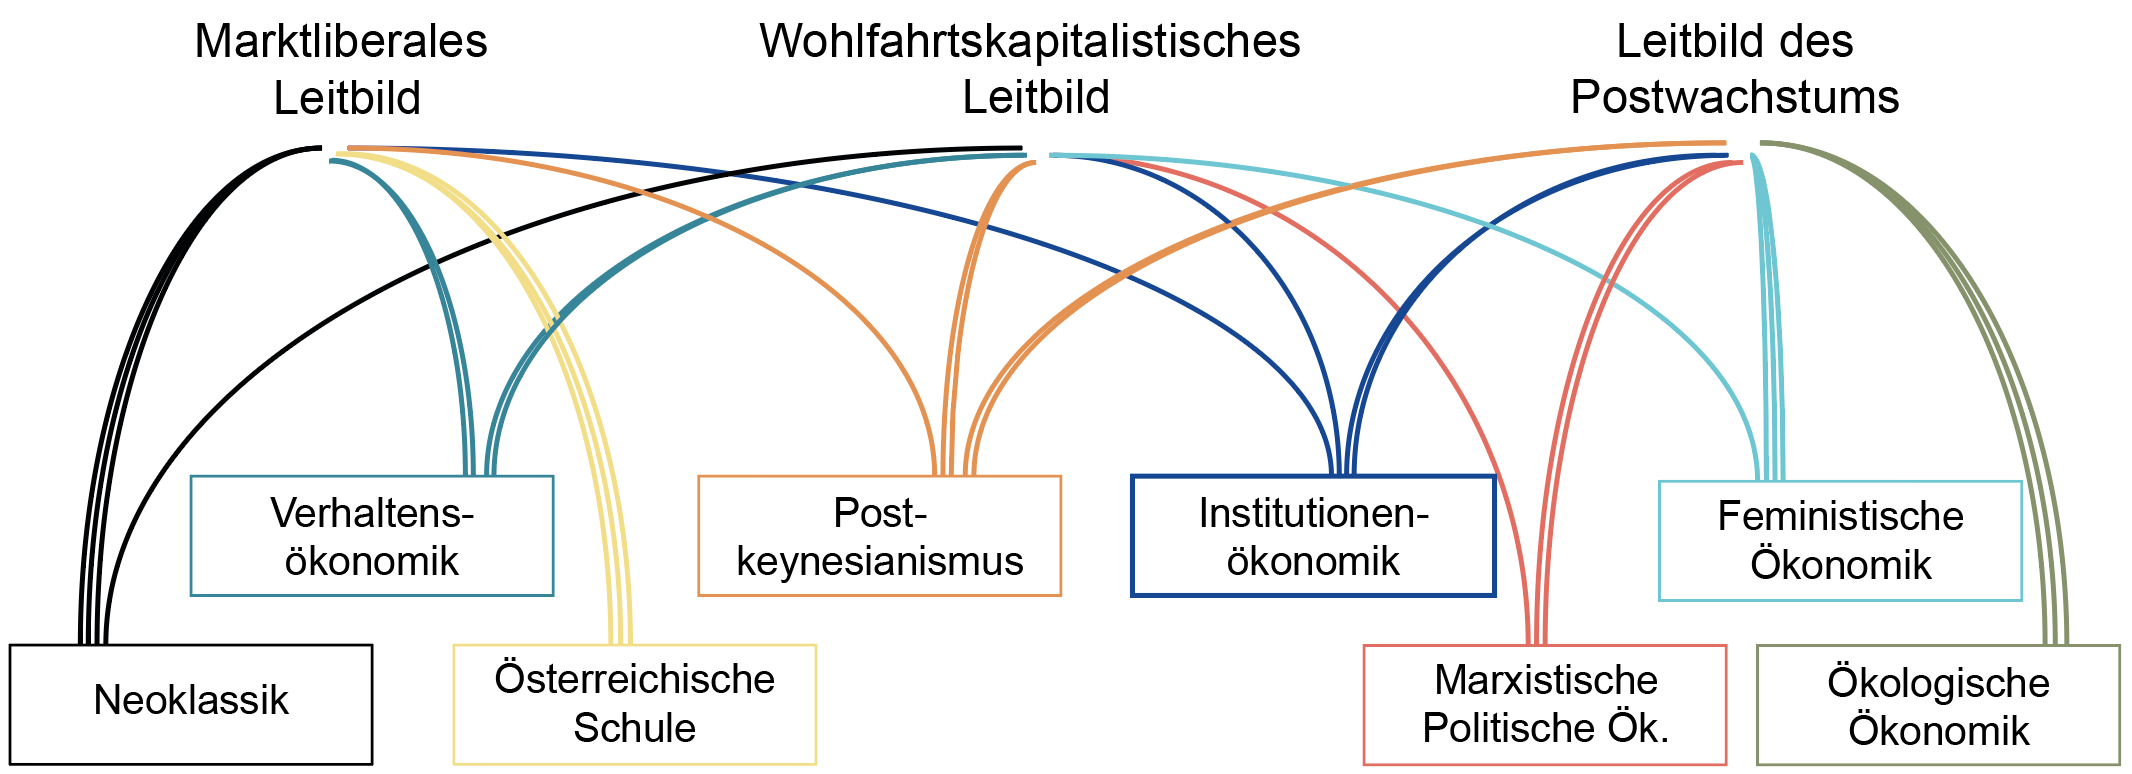
\includegraphics[keepaspectratio]{5_state-and-guiding-models/images/fig2.png}}

}

\caption{Economic policy guiding models and schools of thought. Source:
Own illustration based on the illustrations of
\href{https://www.exploring-economics.org/en/}{Exploring Economics}.}

\end{figure}%

\chapter{Sustainable Economics:
Synthesis}\label{sustainable-economics-synthesis}

\begin{tcolorbox}[enhanced jigsaw, arc=.35mm, bottomrule=.15mm, bottomtitle=1mm, breakable, colback=white, colbacktitle=quarto-callout-note-color!10!white, colframe=quarto-callout-note-color-frame, coltitle=black, left=2mm, leftrule=.75mm, opacityback=0, opacitybacktitle=0.6, rightrule=.15mm, title={Guiding question}, titlerule=0mm, toprule=.15mm, toptitle=1mm]

How can we build a coherent answer to our initial question from
everything we have learned so far -- how can we, as a society, achieve
prosperity within ecological limits?

\end{tcolorbox}

At the end of Chapter 1, we announced that this script follows the
\textbf{sustainable economics} approach -- and deliberately left open
what that means in concrete terms. We noted at the time that sustainable
economics does not start with a fixed answer (``more green growth'' or
``shrinkage'') but with the \textbf{goals} of economic activity itself.
Ever since, we have pursued precisely this question -- what the goal of
economic activity actually is -- throughout the script.

In this final chapter, we bring these threads together. Sustainable
economics is not a further, fourth guiding model alongside market
liberalism, welfare capitalism, and post-growth. Rather, it is a
framework that derives what is needed from the goals themselves, and it
therefore cuts across the guiding models discussed so far. We now make
this approach concrete along three goals -- global ecological justice, a
good life for all, and growth independence -- and six core elements.
Together, they allow us to give a coherent answer to the initial
question of this script: how must an economy be designed so that it
actually achieves its real purpose?

Drawing on Schmelzer and Vetter (2019) and Rogall (2012), sustainable
economics can be captured through three goals:

\begin{itemize}
\item
  \textbf{Global ecological justice}: This includes environmental and
  climate justice, as well as debates on post-extractivism, that is, the
  critique of resource-intensive logics of extraction and export (Acosta
  2017), and post-development approaches that question the Western
  development model as Eurocentric and normative (Klapeer et al. 2023).
\item
  \textbf{A good life for all}: not growth as an end in itself, but an
  economy that meets real needs.
\item
  \textbf{Growth independence}: The ability of an economy to fulfil its
  core functions (employment, social security, public finances) without
  structurally depending on continuous GDP growth.
\end{itemize}

These three goals are deliberately not built on a logic of growth or
shrinkage. They leave open whether and where growth takes place, as long
as the three goals are achieved. This is precisely where their bridging
function lies: sustainable economics does not ask ``growth: yes or no?''
but \emph{``what is needed to make ecological justice and a good life
for all possible, regardless of whether the economy grows, stagnates, or
shrinks in the process?''}

\section{Six Core Elements}\label{six-core-elements}

Following Rogall (2012) and Novy et al. (2020; 2023), the approach can
be made concrete in six core elements:

\begin{enumerate}
\def\labelenumi{\arabic{enumi}.}
\item
  \textbf{Strong rather than weak sustainability}: Natural capital can
  be substituted by manufactured or human capital only to a limited
  extent.
\item
  \textbf{Pluralist approach}: Sustainable economics does not draw on a
  single economic theory. Instead, it integrates ecological,
  institutional, feminist, and post-Keynesian perspectives.
\item
  \textbf{Sustainability paradigm rather than growth paradigm}: This is
  the real controversy in the growth debate: How can the growth paradigm
  be replaced by a sustainability paradigm? The answer is ``selective
  growth'': sectors that contribute to sustainability goals (such as
  renewable energy, care, and education) can grow, while others (such as
  fossil fuels and armaments) must shrink. Growth thus turns from a goal
  into a dependent variable.
\item
  \textbf{Ethical principles}: Precaution rather than remediation, and
  intra- and intergenerational justice rather than pure Pareto
  efficiency. The concern is not only efficiency goals but explicitly
  also questions of distribution. Responsibility is understood in two
  ways here: as consumer sovereignty (responsibility for oneself) and as
  responsibility for the environment and the more-than-human world.
\item
  \textbf{Changing the framework conditions}: political and legal
  instruments such as standard-price approaches or cap-and-trade, merit
  goods, and a sustainable economic policy, for example financing work
  rather than unemployment, reducing working time, and promoting the
  regional economy.
\item
  \textbf{Inter- and transdisciplinary collaboration}: The complexity of
  the challenges requires collaboration across disciplinary boundaries,
  between science, politics, and society.
\end{enumerate}

\section{Outlook: Approaches in the Self-Study
Phase}\label{outlook-approaches-in-the-self-study-phase}

In the following self-study phases, we want to look more closely at
possible approaches to sustainable economics and explore how we can
achieve its goals. We will see that the possible approaches differ
depending on which political guiding model we take as our basis. We will
focus on approaches within the welfare-capitalist guiding model and the
post-growth guiding model, since, in our view, the market-liberal
guiding model lies largely outside sustainable economics. In the next
self-study phase, we will address the following approaches:

Welfare-capitalist guiding model:

\begin{itemize}
\item
  Green growth
\item
  Circular economy
\end{itemize}

Post-growth guiding model:

\begin{itemize}
\item
  Growth-independent institutions
\item
  Sufficient lifestyles
\item
  Collective action
\item
  Caring economy
\item
  Overcoming the imperial mode of living
\end{itemize}

\begin{tcolorbox}[enhanced jigsaw, arc=.35mm, bottomrule=.15mm, bottomtitle=1mm, breakable, colback=white, colbacktitle=quarto-callout-caution-color!10!white, colframe=quarto-callout-caution-color-frame, coltitle=black, left=2mm, leftrule=.75mm, opacityback=0, opacitybacktitle=0.6, rightrule=.15mm, title={Further reading}, titlerule=0mm, toprule=.15mm, toptitle=1mm]

If you are interested, you can watch
\href{https://www.youtube.com/watch?v=2rYNewZEazA&t=1129s}{the statement
by Paolo Gentiloni} (European Commissioner for Economy) at the Beyond
Growth conference to illustrate the green growth position.

The post-growth position is well illustrated in
\href{https://www.youtube.com/watch?v=vij3Q6bE6X4}{a talk by Timothée
Parrique} at the same conference.

\end{tcolorbox}

\bookmarksetup{startatroot}

\chapter*{References}\label{references}
\addcontentsline{toc}{chapter}{References}

\markboth{References}{References}

\protect\phantomsection\label{refs}
\begin{CSLReferences}{1}{1}
\bibitem[\citeproctext]{ref-acostaPostExtractivismDiscoursePractice2017}
Acosta, Alberto. 2017. {`Post-Extractivism: From Discourse to
Practice---Reflections for Action'}. \emph{International Development
Policy \textbar{} Revue Internationale de Politique de Développement},
no. 9: 77--101. \url{https://doi.org/10/ggh26b}.

\bibitem[\citeproctext]{ref-althouseEcologicallyUnequalExchange2023}
Althouse, Jeffrey, Louison Cahen-Fourot, Bruno Carballa-Smichowski,
Cédric Durand, and Steven Knauss. 2023. {`Ecologically Unequal Exchange
and Uneven Development Patterns Along Global Value Chains'}. \emph{World
Development} 170: 106308.
\url{https://doi.org/10.1016/j.worlddev.2023.106308}.

\bibitem[\citeproctext]{ref-anievasHowWestCame2015a}
Anievas, Alexander, and Kerem Nişancıoğlu. 2015. \emph{How the West came
to rule: the geopolitical origins of capitalism}. Pluto Press.

\bibitem[\citeproctext]{ref-atkinsonEconomicsMoralScience2009}
Atkinson, Anthony B. 2009. {`Economics as a Moral Science'}.
\emph{Economica} 76: 791--804.
\url{https://doi.org/10.1111/j.1468-0335.2009.00788.x}.

\bibitem[\citeproctext]{ref-bafuKreislaufwirtschaft2019}
BAFU. 2019. {`Kreislaufwirtschaft'}. In \emph{Bundesamt Für Umwelt
(BAFU)}. \url{https://www.bafu.admin.ch/de/kreislaufwirtschaft}.

\bibitem[\citeproctext]{ref-bauerleGrundfragenOkonomie2026}
Bäuerle, Lukas, Anna Katharina Keil, Rouven Reinke, and Stella Wasenitz,
eds. 2026. \emph{Grundfragen Der {Ökonomie}}. 1. Auflage.
Schäffer-Poeschel Verlag.

\bibitem[\citeproctext]{ref-streckeisenUnsichtbarenPrekaritaetZur2019}
Baumgartner, A. Doris, Beat Fux, and Peter Streckeisen. 2019. {`Von der
unsichtbaren Prekarität zur Beschäftigung ohne Qualität. Politische
Programmatik und das Streben nach kognitiver Hegemonie'}. In
\emph{Sozialstaat unter Zugzwang?: Zwischen Reform und radikaler
Neuorientierung}. Springer Fachmedien Wiesbaden.
\url{http://link.springer.com/10.1007/978-3-658-22444-8}.

\bibitem[\citeproctext]{ref-beckertKapitalismusGeschichteWeltrevolution2026}
Beckert, Sven, and Helmut Dierlamm. 2026. \emph{Kapitalismus: Geschichte
einer Weltrevolution}. 3. Auflage, deutsche Erstausgabe. Rowohlt.

\bibitem[\citeproctext]{ref-benelliWenigerWertTemporar2014}
Benelli, Natalie, and Peter Streckeisen. 2014. {`Weniger Wert? Temporär
Beschäftigte in Der Schweiz'}.

\bibitem[\citeproctext]{ref-bernetArbeitAndersDenken2021}
Bernet, Brigitta. 2021. {`Arbeit Anders Denken'}. In
\emph{Sozialalmanach 2021: Armut Grenzt Aus}. Caritas.

\bibitem[\citeproctext]{ref-bfsLIK2026}
BFS. 2026. \emph{Landesindex Der {Konsumentenpreise} ({LIK})}. Bundesamt
für Statistik (BFS).
\href{https://www.LIK.bfs.admin.ch}{www.LIK.bfs.admin.ch}.

\bibitem[\citeproctext]{ref-binswangerWachstumszwangWarumVolkswirtschaft2019}
Binswanger, Mathias. 2019. \emph{Der Wachstumszwang: warum die
Volkswirtschaft immer weiterwachsen muss, selbst wenn wir genug haben}.
Wiley-VCH Verlag GmbH \& Co. KGaA.

\bibitem[\citeproctext]{ref-bontrupVolkswirtschaftslehreAusOrthodoxer2021a}
Bontrup, Heinz-J., and Ralf-M. Marquardt. 2021.
\emph{Volkswirtschaftslehre Aus Orthodoxer Und Heterodoxer Sicht}. De
Gruyter Oldenbourg.

\bibitem[\citeproctext]{ref-ceasarPlanetaryHealthCheck2024}
Ceasar, L., B. Sakschweski, L. S. Andersen, et al. 2024. \emph{Planetary
Health Check Report 2024}. Potsdam Institute for Climate Impact
Research.

\bibitem[\citeproctext]{ref-changKickingAwayLadder2002}
Chang, Ha-Joon. 2002. \emph{Kicking Away the Ladder: Development
Strategy in Historical Perspective}. 1st ed. Anthem Press.

\bibitem[\citeproctext]{ref-changLifeUniverseEverything2014}
Chang, Ha-Joon, and Ha-Joon Chang. 2014. {`Life, the Universe and
Everything. What Is Economics?'} In \emph{Economics: The User's Guide}.
Bloomsbury Press.

\bibitem[\citeproctext]{ref-palmaLatinAmericanEconomies2003}
Chang, Ha-Joon, and Jose Gabriel Palma. 2003. {`The Latin American
Economies During the Second Half of the Twentieth Century - from the Age
Og 'ISI' to the Age of 'the End of History''}. In \emph{Rethinking
Development Economics}. Anthem Press.

\bibitem[\citeproctext]{ref-coaseProblemSocialCost1960}
Coase, Ronald H. 1960. {`The Problem of Social Cost'}. \emph{The Journal
of Law \& Economics} 3: 1--44.

\bibitem[\citeproctext]{ref-corakIncomeInequalityEquality2013}
Corak, Miles. 2013. {`Income {Inequality}, {Equality} of {Opportunity},
and {Intergenerational Mobility}'}. \emph{Journal of Economic
Perspectives} 27 (3): 79--102.
\url{https://doi.org/10.1257/jep.27.3.79}.

\bibitem[\citeproctext]{ref-dalisaNachwortAusteritaetZur2016}
D'Alisa, Giacoma, Giorgos Kallis, and Federico Demaria. 2016.
{`Nachwort: {Von} Der {Austerität} Zur {Dépense}'}. In \emph{Degrowth:
{Handbuch} Für Eine Neue Ära}, edited by Giacoma D'Alisa, Federico
Demaria, and Giorgios Kallis. Oekom Verlag.

\bibitem[\citeproctext]{ref-dalyNewEconomicsOur2017}
Daly, Herman. 2017. {`A New Economics for Our Full World'}.
\emph{Victor, P., Dolter, B., Handbook of Growth and Sustainability.
Cheltenham: Edward Elgar}, 85--106.

\bibitem[\citeproctext]{ref-daoWhyLaborReceiving2017}
Dao, Mai, Mitali Das, Zsoka Koczan, and Weicheng Lian. 2017. {`Why {Is}
{Labor} {Receiving} a {Smaller} {Share} of {Global} {Income}? {Theory}
and {Empirical} {Evidence}'}. \emph{IMF Working Papers} 2017 (169).
\url{https://doi.org/10.5089/9781484311042.001}.

\bibitem[\citeproctext]{ref-davisLateVictorianHolocausts2017a}
Davis, Mike. 2017. \emph{Late Victorian holocausts: El Niño famines and
the making of the Third World}. Paperback edition. Verso.

\bibitem[\citeproctext]{ref-dekeyzerInclusiveCommonsSustainability2018}
De Keyzer, Maïka. 2018. \emph{Inclusive Commons and the Sustainability
of Peasant Communities in the Medieval Low Countries}. Routledge.

\bibitem[\citeproctext]{ref-demoorDilemmaCommonersUnderstanding2015}
De Moor, Tine. 2015. \emph{The Dilemma of the Commoners: Understanding
the Use of Common-Pool Resources in Long-Term Perspective}. Cambridge
University Press.
\url{https://www.cambridge.org/core/books/dilemma-of-the-commoners/BA497A670AD2F573178D89947EC38F7D}.

\bibitem[\citeproctext]{ref-davisEconomistsOddStand2016}
DeMartino, George F., Deirdre McCloskey, John B. Davis, and John B.
Davis. 2016. {`Economists' Odd Stand on the Positive--Normative
Distinction: A Behavioral Economics View'}. In \emph{The Oxford Handbook
of Professional Economic Ethics}. Oxford University Press.
\url{https://academic.oup.com/edited-volume/28011/chapter/211790248}.

\bibitem[\citeproctext]{ref-dorningerGlobalPatternsEcologically2021a}
Dorninger, Christian, Alf Hornborg, David J. Abson, et al. 2021.
{`Global Patterns of Ecologically Unequal Exchange: Implications for
Sustainability in the 21st Century'}. \emph{Ecological Economics} 179:
106824. \url{https://doi.org/10.1016/j.ecolecon.2020.106824}.

\bibitem[\citeproctext]{ref-durandIntellectualMonopolyGlobal2020a}
Durand, Cédric, and Wiliiam Milberg. 2020. {`Intellectual Monopoly in
Global Value Chains'}. \emph{Review of International Political Economy}
27 (2): 404--29. \url{https://doi.org/10.1080/09692290.2019.1660703}.

\bibitem[\citeproctext]{ref-eeaEuropeanEnvironmentState2015}
EEA. 2015. \emph{The {European} Environment --- State and Outlook 2015:
Synthesis Report}. European Environment Agency (EEA).
\url{https://doi.org/10.2800/944899}.

\bibitem[\citeproctext]{ref-elsonProgressWomenEmpowerment2000}
Elson, Diane. 2000. {`The {Progress} of {Women}: {Empowerment} and
{Economics}'}. In \emph{Progress of the {World}'s {Women} 2000: {UNIFEM}
{Biennial} {Report}}, edited by Karen Judd. United Nations Development
Fund for Women (UNIFEM).

\bibitem[\citeproctext]{ref-engelkampEinfuehrungVolkswirtschaftslehre2013}
Engelkamp, Paul, and Friedrich L. Sell. 2013. \emph{Einführung in die
Volkswirtschaftslehre}. 6., überarbeitete und erweiterte Aufl age.
Springer Berlin Heidelberg.
\url{https://link.springer.com/10.1007/978-3-642-36522-5}.

\bibitem[\citeproctext]{ref-famaEfficientCapitalMarkets1970}
Fama, Eugene F. 1970. {`Efficient {Capital} {Markets}: {A} {Review} of
{Theory} and {Empirical} {Work}'}. \emph{The Journal of Finance} 25 (2):
383. \url{https://doi.org/10.2307/2325486}.

\bibitem[\citeproctext]{ref-fisherPurchasingPowerMoney1922a}
Fisher, Irving. 1922. \emph{The Purchasing Power of Money, Its
Determination and Relation to Credit, Interest and Crises}. Macmillan.

\bibitem[\citeproctext]{ref-fraserRethinkingPublicSphere1990}
Fraser, Nancy. 1990. {`Rethinking the {Public} {Sphere}: {A}
{Contribution} to the {Critique} of {Actually} {Existing} {Democracy}'}.
\emph{Social Text}, no. 25/26: 56--80.
\url{https://doi.org/10.2307/466240}.

\bibitem[\citeproctext]{ref-fraserCannibalCapitalismHow2022}
Fraser, Nancy. 2022. \emph{Cannibal {Capitalism}: {How} {Our} {System}
{Is} {Devouring} {Democracy}, {Care}, and the {Planet} - and {What} {We}
{Can} {Do} about {It}}. Verso.

\bibitem[\citeproctext]{ref-friedliBetriebswirtschaftslehreZusammenhangeVerstehen2019}
Friedli, Vera, Renato Müller Vasquez Callo, and Rahel Balmer-Zahnd.
2019. \emph{Betriebswirtschaftslehre: Zusammenhänge Verstehen}. 4.
Auflage. Hep Verlag AG.

\bibitem[\citeproctext]{ref-friedmanMethodologyPositiveEconomics1953a}
Friedman, Milton. 1953. \emph{The Methodology of Positive Economics}.
University of Chicago.
\url{https://www.marxists.org/reference/subject/philosophy/works/us/friedman.htm}.

\bibitem[\citeproctext]{ref-ghoshNutmegsCurseParables2021}
Ghosh, Amitav. 2021. \emph{The Nutmeg's Curse: Parables for a Planet in
Crisis}. University of Chicago Press.

\bibitem[\citeproctext]{ref-greenWhatsHappeningGlobal2016}
Green, Duncan. 2016. {`What's Happening on {Global} {Inequality}?
{Putting} the {``Elephant Graph''} to Sleep with a {``Hockey Stick''}'}.
In \emph{From Poverty to Power}.
\url{https://frompoverty.oxfam.org.uk/whats-happening-on-global-inequality-putting-the-elephant-graph-to-sleep-with-a-hockey-stick/}.

\bibitem[\citeproctext]{ref-degenArbeitUndKapital2012}
Halbeisen, Patrick, Margrit Müller, Béatrice Veyrassat, and Bernard
Degen. 2012. {`Arbeit Und Kapital'}. In \emph{Wirtschaftsgeschichte Der
Schweiz Im 20. Jahrhundert}. Schwabe Verlag.

\bibitem[\citeproctext]{ref-hardinTragedyCommons1968}
Hardin, Garrett. 1968. {`The Tragedy of the Commons'}. \emph{Science}
162 (3859): 1243--48.
\url{https://doi.org/10.1126/science.162.3859.1243}.

\bibitem[\citeproctext]{ref-harveyBriefHistoryNeoliberalism2005}
Harvey, David. 2005. \emph{A {Brief} {History} of {Neoliberalism}}.
Oxford Scholarship Online. Oxford University Press.
\url{https://doi.org/10.1093/oso/9780199283262.001.0001}.

\bibitem[\citeproctext]{ref-bowlesWelcheGueterSollen2014}
Herzog, Lisa, Samuel Bowles, and Axel Honneth. 2014. {`Welche Güter
sollen in Märkten gehandlet werden? Was Märkte können - und was nicht'}.
In \emph{Der Wert des Marktes: ein ökonomisch-philosophischer Diskurs
vom 18. Jahrhundert bis zur Gegenwart}. Suhrkamp.

\bibitem[\citeproctext]{ref-hickelDivideBriefGuide2017}
Hickel, Jason. 2017. \emph{The Divide - a Brief Guide to Global
Inequality and Its Solutions}. William Heinemann.

\bibitem[\citeproctext]{ref-hillAdamSmithThumos2012a}
Hill, Lisa. 2012. {`Adam Smith on 'Thumos' and Irrational Economic
{``Man''}'}. \emph{The European Journal of the History of Economic
Thought} 19 (1): 1--22. \url{https://doi.org/10.1080/09672561003632550}.

\bibitem[\citeproctext]{ref-hodgsonWhatCapital2014}
Hodgson, Geoffrey M. 2014. {`What Is Capital? {Economists} and
Sociologists Have Changed Its Meaning: Should It Be Changed Back?'}
\emph{Cambridge Journal of Economics} 38 (5): 1063--86.
\url{https://doi.org/10.1093/cje/beu013}.

\bibitem[\citeproctext]{ref-huberFuelingCapitalismOil2013}
Huber, Matt. 2013. {`Fueling Capitalism: Oil, the Regulation Approach,
and the Ecology of Capital'}. \emph{Economic Geography} 89 (2): 171--94.
\url{https://doi.org/10.1111/ecge.12006}.

\bibitem[\citeproctext]{ref-jacksonProsperityGrowthTransition2009}
Jackson, Tim. 2009. \emph{Prosperity Without Growth? {The} Transition to
a Sustainable Economy}. Sustainable Development Commission.

\bibitem[\citeproctext]{ref-jarrigeContaminationEarthHistory2020}
Jarrige, François, Thomas Le Roux, Janice Egan, and Michael Egan. 2020.
\emph{The Contamination of the Earth: A History of Pollutions in the
Industrial Age}. The MIT Press.

\bibitem[\citeproctext]{ref-jevonsTheoryPoliticalEconomy1879}
Jevons, William Stanley. 1879. \emph{The Theory of Political Economy}.
2nd edn. Macmillan.

\bibitem[\citeproctext]{ref-johnstonBriefHistoryJustice2011}
Johnston, David. 2011. \emph{A {Brief} {History} of {Justice}}. Brief
{Histories} of {Philosophy}. Wiley-Blackwell.
\url{https://doi.org/10.1002/9781444397550}.

\bibitem[\citeproctext]{ref-kalaitzakisFunctionalPersonalIncome2026}
Kalaitzakis, Alexandros, and Christos Papatheodorou. 2026. {`Functional
and Personal Income Distribution and Their Effect on Demand: An
Empirical Assessment on the {EU}-15 Countries'}. \emph{Journal of Post
Keynesian Economics} 49 (3): 560--604.
\url{https://doi.org/10.1080/01603477.2026.2626368}.

\bibitem[\citeproctext]{ref-kaleckiPoliticalAspectsFull1943}
Kalecki, Michal. 1943. {`The {Political} {Aspects} of {Full}
{Employment}'}. \emph{The Political Quarterly} 14 (4): 322--30.
\url{https://doi.org/10.1111/j.1467-923X.1943.tb01016.x}.

\bibitem[\citeproctext]{ref-kallisOilEconomySystematic2017}
Kallis, Giorgos, and Jalel Sager. 2017. {`Oil and the Economy: A
Systematic Review of the Literature for Ecological Economists'}.
\emph{Ecological Economics} 131: 561--71.
\url{https://doi.org/10.1016/j.ecolecon.2016.08.011}.

\bibitem[\citeproctext]{ref-kappEnvironmentalPoliciesDevelopment1974}
Kapp, K. William. 1974. \emph{Environmental Policies and Development
Planning in Contemporary China and Other Essays}. De Gruyter.
\url{https://www.degruyter.com/document/doi/10.1515/9783112317273/html}.

\bibitem[\citeproctext]{ref-kappSocialCostsPrivate1950}
Kapp, William. 1950. \emph{The Social Costs of Private Enterprise}.
Harvard University Press.

\bibitem[\citeproctext]{ref-keenDebunkingEconomicsNaked2010}
Keen, Steve. 2010. \emph{Debunking economics: the naked emperor of the
social sciences}. 5. impression. Zed Books.

\bibitem[\citeproctext]{ref-keynesENDLAISSEZFAIRE19261978}
Keynes, John Maynard. 1978. {`{THE} {END} {OF} {LAISSEZ}-{FAIRE}
(1926)'}. In \emph{The {Collected} {Writings} of {John} {Maynard}
{Keynes}}, edited by Donald Moggridge and Elizabeth Johnson, Volume 9:
Essays in Persuasion. Royal Economic Society.
\url{https://doi.org/10.1017/UPO9781139524162.027}.

\bibitem[\citeproctext]{ref-klapeerPostDevelopment2023}
Klapeer, Christine M., Karin Fischer, Gerhard Hauck, and Manuela Boatcă.
2023. {`Post-Development'}. In \emph{Handbuch Entwicklungsforschung}.
Springer Fachmedien. \url{https://doi.org/10.1007/978-3-658-32946-4_12}.

\bibitem[\citeproctext]{ref-kubiszewskiGDPMeasuringAchieving2013}
Kubiszewski, Ida, Robert Costanza, Carol Franco, et al. 2013. {`Beyond
GDP: Measuring and Achieving Global Genuine Progress'}. \emph{Ecological
Economics} 93: 57--68.
\url{https://doi.org/10.1016/j.ecolecon.2013.04.019}.

\bibitem[\citeproctext]{ref-lannenInequalityWhatsWord2019}
Lannen, Anu, Sabin Bieri, and Christoph Bader. 2019. \emph{Inequality:
What?s in a Word?} Centre for Development; Environment (CDE), University
of Bern. \url{https://boris.unibe.ch/130698/}.

\bibitem[\citeproctext]{ref-lawrenceGlobalPolycrisisCausal2024a}
Lawrence, Michael, Thomas Homer-Dixon, Scott Janzwood, Johan Rockstöm,
Ortwin Renn, and Jonathan F. Donges. 2024. {`Global Polycrisis: The
Causal Mechanisms of Crisis Entanglement'}. \emph{Global Sustainability}
7: e6. \url{https://doi.org/10.1017/sus.2024.1}.

\bibitem[\citeproctext]{ref-lepeniesMachtZahlPolitische2013}
Lepenies, Philipp. 2013. \emph{Die Macht Der Einen Zahl: Eine Politische
Geschichte Des Bruttoinlandsprodukts}. Erste Auflage, Originalausgabe.
Suhrkamp.

\bibitem[\citeproctext]{ref-lessenichNebenUnsSintflut2018}
Lessenich, Stephan. 2018. \emph{Neben Uns Die Sintflut: Wie Wir Auf
Kosten Anderer Leben}.

\bibitem[\citeproctext]{ref-lessenichNebenUnsSintflut2020}
Lessenich, Stephan. 2020. \emph{Neben uns die Sintflut: die
Externalisierungsgesellschaft und ihr Preis}. 6. Auflage. Hanser Berlin.

\bibitem[\citeproctext]{ref-magdoffDisposableWorkersTodays2004}
Magdoff, Fred, and Harry Magdoff. 2004. {`Disposable Workers: Today's
Reserve Army of Labor'}. \emph{Monthly Review} 55 (11): 18.
\url{https://doi.org/10.14452/MR-055-11-2004-04_2}.

\bibitem[\citeproctext]{ref-maitlandResistingRuleRich2026}
Maitland, Alex, Anjela Taneja, Anthony Kamande, et al. 2026.
\emph{Resisting the {Rule} of the {Rich}}. Oxfam International.
\url{https://doi.org/10.21201/2025.000113}.

\bibitem[\citeproctext]{ref-malmFossilCapitalRise2016}
Malm, Andreas. 2016. \emph{Fossil capital: the rise of steam-power and
the roots of global warming}. Verso.

\bibitem[\citeproctext]{ref-mankiwEconomics2020}
Mankiw, Nicholas Gregory, and Mark P. Taylor. 2020. \emph{Economics}.
Fifth edition. Cengage.

\bibitem[\citeproctext]{ref-marshallIndustryTradeStudy1919}
Marshall, Alfred. 1919. \emph{Industry and Trade: A Study of Industrial
Technique and Business Organization; and of Their Influences on the
Conditions of Various Classes and Nations}. Macmillan.

\bibitem[\citeproctext]{ref-marshallPrinciplesEconomics2013}
Marshall, Alfred. 2013. \emph{Principles of Economics}. 8th edn.
Palgrave Macmillan UK.

\bibitem[\citeproctext]{ref-maslowPsychologyScience1966}
Maslow, Abraham H. 1966. \emph{The Psychology of Science: A
Reconnaissance}. Harper \& Row.

\bibitem[\citeproctext]{ref-matteiKurzePhanomenologieCommons2014}
Mattei, Ugo. 2014. {`Eine Kurze {Phänomenologie} Der {Commons}'}. In
\emph{Commons}, edited by Silke Helfrich and Heinrich-Böll-Stiftung.
Transcript Verlag. \url{https://doi.org/10.14361/9783839428351-010}.

\bibitem[\citeproctext]{ref-mazzucatoValueEverythingMaking2018}
Mazzucato, Mariana. 2018. \emph{The Value of Everything: Making and
Taking in the Global Economy}. Hachette UK.

\bibitem[\citeproctext]{ref-mazzucatoMissionEconomyMoonshot2022}
Mazzucato, Mariana. 2022. \emph{Mission economy: a moonshot guide to
changing capitalism}. Penguin Books.

\bibitem[\citeproctext]{ref-milanovicTwoFacesGlobalization2003}
Milanovic, Branko. 2003. {`The Two Faces of Globalization: Against
Globalization as We Know It'}. \emph{World Development} 31 (4): 667--83.
\url{https://doi.org/10.1016/S0305-750X(03)00002-0}.

\bibitem[\citeproctext]{ref-minskyFinancialInstabilityHypothesis1992}
Minsky, Hyman. 1992. \emph{The Financial Instability Hypothesis}. No.
74. The Jerome Levy Economics Institute of Bard College.

\bibitem[\citeproctext]{ref-mirowskiMoreHeatLight1989a}
Mirowski, Philip. 1989. \emph{More Heat Than Light: Economics as Social
Physics, Physics as Nature's Economics}. Cambridge University Press.
\url{https://www.cambridge.org/core/books/more-heat-than-light/4CD2ADE8D5DE8665E43E2922D7E360B3}.

\bibitem[\citeproctext]{ref-morganEconomicManModel2006a}
Morgan, Mary S. 2006. {`Economic Man as Model Man: Ideal Types,
Idealization and Caricatures'}. \emph{Journal of the History of Economic
Thought} 28 (1): 1--27. \url{https://doi.org/10.1080/10427710500509763}.

\bibitem[\citeproctext]{ref-morganWorldModelHow2012b}
Morgan, Mary S. 2012. \emph{The World in the Model: How Economists Work
and Think}. Cambridge University Press.
\url{https://www.cambridge.org/core/books/world-in-the-model/6FD82E4D498F94CBE5F56078FD007729}.

\bibitem[\citeproctext]{ref-nordhausClimateChangeUltimate2019}
Nordhaus, William. 2019. {`Climate Change: The Ultimate Challenge for
Economics'}. \emph{American Economic Review} 109 (6): 1991--2014.
\url{https://doi.org/10.1257/aer.109.6.1991}.

\bibitem[\citeproctext]{ref-novyZukunftfahigesWirtscchaften2020}
Novy, Andreas, Richard Bärnthaler, and Veronika Heimerl. 2020.
\emph{Zukunftfähiges Wirtscchaften}. Beltz Juventa.

\bibitem[\citeproctext]{ref-novyZukunftsfaehigesWirtschaften2023}
Novy, Andreas, Richard Bärnthaler, and Magdalena Prieler. 2023.
\emph{Zukunftsfähiges Wirtschaften: Herausforderungen der
sozialökologischen Transformation}. 2. Auflage. Juventa Verlag.

\bibitem[\citeproctext]{ref-nubbemeyerReconsiderationFullCostPricing2010}
Nubbemeyer, Elmar. 2010. {`A Reconsideration of Full-Cost Pricing -
Methodological Aspects of Marginalism and Theoretical Explanations of
Pricing Behaviour'}. PhD thesis, Ludwig-Maximilians-Universität.

\bibitem[\citeproctext]{ref-nussbaumCapabilitiesFundamentalEntitlements2003}
Nussbaum, Martha. 2003. {`Capabilites as Fundamental Entitlements: Sen
and Social Justice'}. \emph{Feminist Economics} 9 (2/3): 33--59.

\bibitem[\citeproctext]{ref-oecdGreenGrowth2011}
OECD. 2011. \emph{Towards {Green} {Growth}}. OECD Publishing.
\url{https://doi.org/10.1787/9789264111318-en}.

\bibitem[\citeproctext]{ref-ostromMarketsStatesPolycentric2010}
Ostrom, Elinor. 2010. {`Beyond {Markets} and {States}: {Polycentric}
{Governance} of {Complex} {Economic} {Systems}'}. \emph{American
Economic Review} 100 (3): 1--33.

\bibitem[\citeproctext]{ref-ottTheorieUndPraxis2004}
Ott, Konrad, and Ralf Döring. 2004. \emph{Theorie Und Praxis Starker
Nachhaltigkeit}. Metropolis.

\bibitem[\citeproctext]{ref-paechBefreiungVomUberfluss2012}
Paech, Niko. 2012. \emph{Befreiung Vom Überfluss. Auf Dem Weg in Die
Postwachstumsökonomie}. München.

\bibitem[\citeproctext]{ref-paretoAnwendungenMathematikAuf1902}
Pareto, Vilfredo, and Wilhelm Franz Meyer. 1902. {`Anwendungen Der
Mathematik Auf Nationalokonomie'}. In \emph{Encyklopädie Der
Mathematischen Wissenschaften Mit Einschluss Ihrer Anwendungen}. B.G.
Teubner.

\bibitem[\citeproctext]{ref-patnaikCapitalImperialismTheory2021}
Patnaik, Utsa, and Prabhat Patnaik. 2021. \emph{Capital and Imperialism:
Theory, History, and the Present}. Monthly Review Press.

\bibitem[\citeproctext]{ref-petschowGesellschaftlichesWohlergehenInnerhalb2018}
Petschow, Ulrich, Eugen Pissarskoi, Nils aus dem Moore, Hermann Ott, and
Umweltbundesamt. 2018. \emph{Gesellschaftliches Wohlergehen innerhalb
planetarer Grenzen: Der Ansatz einer vorsorgeorientierten
Postwachstumsposition}. No. 89. Umweltbundesamt.

\bibitem[\citeproctext]{ref-pikettyCapitalTwentyFirstCentury2014}
Piketty, Thomas, and Arthur Goldhammer. 2014. \emph{Capital in the
twenty-first century}. The Belknap Press of Harvard University Press.

\bibitem[\citeproctext]{ref-pirgmaierNeoclassicalTrojanHorse2017}
Pirgmaier, Elke. 2017. {`The Neoclassical Trojan Horse of Steady-State
Economics'}. \emph{Ecological Economics} 133: 52--61.
\url{https://doi.org/10.1016/j.ecolecon.2016.11.010}.

\bibitem[\citeproctext]{ref-polanyiGreatTransformation2017}
Polanyi, Karl. 2017. \emph{The Great Transformation}. 13. Auflage.
Suhrkamp Taschenbuch Verlag.

\bibitem[\citeproctext]{ref-polanyiEconomyInstitutedProcess1957a}
Polanyi, Karl, Karl Polanyi, Conrad M. Arensberg, and Harry W. Pearson.
1957. {`The Economy as Instituted Process'}. In \emph{Trade and Market
in the Early empires}. The Free Press \& The Falcon's Wing Press.

\bibitem[\citeproctext]{ref-ponteHiddenCostsEnvironmental2022}
Ponte, Stefano. 2022. {`The Hidden Costs of Environmental Upgrading in
Global Value Chains'}. \emph{Review of International Political Economy}
29 (3): 818--43. \url{https://doi.org/10.1080/09692290.2020.1816199}.

\bibitem[\citeproctext]{ref-pufeNachhaltigkeit2017}
Pufé, Iris. 2017. \emph{Nachhaltigkeit}. 3., überarbeitete und
erweiterte Auflage. UVK Verlagsgesellschaft mbH.

\bibitem[\citeproctext]{ref-putnamCollapseFactValue2002}
Putnam, Hilary. 2002. \emph{The Collapse of the Fact-Value Dichotomy and
Other Essays}. Harvard University Press.

\bibitem[\citeproctext]{ref-rawlsTheoryJustice1999}
Rawls, John. 1999. \emph{A {Theory} of {Justice}: {Revised} {Edition}}.
Harvard University Press. \url{https://doi.org/10.2307/j.ctvkjb25m}.

\bibitem[\citeproctext]{ref-raworthDoughnutAnthropoceneHumanitys2017}
Raworth, Kate. 2017. {`A Doughnut for the Anthropocene: Humanity's
Compass in the 21st Century'}. \emph{The Lancet Planetary Health} 1 (2):
e48--49. \url{https://doi.org/10.1016/S2542-5196(17)30028-1}.

\bibitem[\citeproctext]{ref-reissMathematicsEconomicsSchmoller2000a}
Reiss, Julian. 2000. {`Mathematics in Economics: Schmoller, Menger and
Jevons'}. \emph{Journal of Economic Studies} 27 (4/5): 477--91.
\url{https://doi.org/10.1108/01443580010342393}.

\bibitem[\citeproctext]{ref-robbinsEssayNatureSignificance1932}
Robbins, Lionel. 1932. \emph{An Essay on the Nature and Significance of
Economic Science}. Macmillan \& Co. Limited.

\bibitem[\citeproctext]{ref-millEssaysEconomicsSociety1996}
Robson, John M., and John Stuart Mill. 1996. \emph{Essays on Economics
and Society}. University of Toronto Press.

\bibitem[\citeproctext]{ref-rockstromSafeOperatingSpace2009}
Rockström, Johan, Will Steffen, Kevin Noone, et al. 2009. {`A Safe
Operating Space for Humanity'}. \emph{Nature} 461 (7263): 472--75.
\url{https://doi.org/10.1038/461472a}.

\bibitem[\citeproctext]{ref-rogallNachhaltigeOkonomieOkonomische2012}
Rogall, Holger. 2012. \emph{Nachhaltige Ökonomie. Ökonomische Theorie
Und Praxis Einer Nachhaltigen Entwicklung}. 2., überarbeitete und stark
erweiterte Auflage. Metropolis.

\bibitem[\citeproctext]{ref-rogallVolkswirtschaftslehreFuerSozialwissenschaftler2013}
Rogall, Holger. 2013. \emph{Volkswirtschaftslehre Für
{Sozialwissenschaftler}: {Einführung} in Eine Zukunftsfähige
{Wirtschaftslehre}}. 2. Aufl. Lehrbuch. Springer VS.
\url{https://doi.org/10.1007/978-3-658-01980-8}.

\bibitem[\citeproctext]{ref-rosaSocialAccelerationEthical2003a}
Rosa, Hartmut. 2003. {`Social Acceleration: Ethical and Political
Consequences of a Desynchronized High--Speed Society'}.
\emph{Constellations} 10 (1): 3--33.
\url{https://doi.org/10.1111/1467-8675.00309}.

\bibitem[\citeproctext]{ref-rosaBeschleunigungUndEntfremdung2024}
Rosa, Hartmut, and Robin Celikates. 2024. \emph{Beschleunigung und
Entfremdung: Entwurf einer kritischen Theorie spätmoderner
Zeitlichkeit}. 10. Auflage. Suhrkamp.

\bibitem[\citeproctext]{ref-saaveEinverleibenUndExternalisieren2022a}
Saave, Anna, and Friedrich-Schiller-Universität Jena. 2022.
\emph{Einverleiben und Externalisieren: zur Innen-Außen-Beziehung der
kapitalistischen Produktionsweise}. Transcript.

\bibitem[\citeproctext]{ref-sakschewskiPlanetaryHealthCheck2025a}
Sakschewski, Boris, Levke Caesar, Lauren Andersen, et al. 2025.
\emph{Planetary Health Check 2025: A Scientific Assessment of the State
of the Planet}. Potsdam Institute for Climate Impact Research (PIK).
\url{https://publications.pik-potsdam.de/pubman/item/item_32589}.

\bibitem[\citeproctext]{ref-santariusReboundEffektUberUnerwunschten2014}
Santarius, Tilman. 2014. \emph{Der Rebound-Effekt: Über Die
Unerwünschten Folgen Der Erwünschten Energieeffizienz}. Wuppertal
Institut für Klima, Umwelt und Energie.

\bibitem[\citeproctext]{ref-schauppStoffwechselpolitikArbeitNatur2024}
Schaupp, Simon. 2024. \emph{Stoffwechselpolitik: Arbeit, Natur und die
Zukunft des Planeten}. Erste Auflage, Sonderdruck, Originalausgabe.
Suhrkamp.

\bibitem[\citeproctext]{ref-streckeisenSteigendeErwerbslosigkeitUnd2012}
Scherschel, Karin, Peter Streckeisen, Manfred Krenn, and Peter
Streckeisen. 2012. {`Steigende Erwerbslosigkeit Und Prekarität in Der
Schweiz: Das Ende Eines "Sonderfalls"'}. In \emph{Neue Prekarität: Die
Folgen Aktivierender Arbeitsmarktpolitik: Europäische Länder Im
Vergleich}. Campus.

\bibitem[\citeproctext]{ref-schmelzerDegrowthPostwachstum2019}
Schmelzer, Matthias, and Andrea Vetter. 2019.
\emph{Degrowth/Postwachstum}. Junius.

\bibitem[\citeproctext]{ref-sedlacekOekonomieGutUnd2012}
Sedlacek, Tomas. 2012. \emph{Die Ökonomie von Gut Und Böse}. Hanser.

\bibitem[\citeproctext]{ref-seidlPostwachstumsgesellschaftKonzepteFur2010}
Seidl, Irmi, and Angelika Zahrnt, eds. 2010.
\emph{Postwachstumsgesellschaft. {Konzepte} Für Die {Zukunft}}. Ökologie
Und {Wirtschaftsforschung}. Marbug.

\bibitem[\citeproctext]{ref-senCommoditiesCapabilities1999}
Sen, Amartya. 1999. \emph{Commodities and {Capabilities}}. Oxford
University Press.

\bibitem[\citeproctext]{ref-sheldonMigrationIntegrationUnd2007}
Sheldon, George. 2007. \emph{Migration, Integration und Wachstum: Die
Performance und wirtschaftliche Auswirkung der Ausländer in der
Schweiz}. 01/07. Center of Business; Economics (WWZ) / Universität
Basel.

\bibitem[\citeproctext]{ref-slobodianGlobalistsEndEmpire2018}
Slobodian, Quinn. 2018. \emph{Globalists: The End of Empire and the
Birth of Neoliberalism}. Harvard University Press,.
\url{https://slsp-ube.primo.exlibrisgroup.com/view/action/uresolver.do?operation=resolveService&package_service_id=28697326480005511&institutionId=5511&customerId=5500&VE=true}.

\bibitem[\citeproctext]{ref-smithWohlstandNationenUntersuchung2013}
Smith, Adam, and Horst Claus Recktenwald. 2013. \emph{Der Wohlstand der
Nationen: eine Untersuchung seiner Natur und seiner Ursachen
{[}1789{]}}. 13. Auflage. Deutscher Taschenbuch Verlag.

\bibitem[\citeproctext]{ref-steffenTrajectoryAnthropoceneGreat2015b}
Steffen, Will, Wendy Broadgate, Lisa Deutsch, Owen Gaffney, and Cornelia
Ludwig. 2015. {`The Trajectory of the Anthropocene: The Great
Acceleration'}. \emph{The Anthropocene Review} 2 (1): 81--98.
\url{https://doi.org/10.1177/2053019614564785}.

\bibitem[\citeproctext]{ref-vazquezMarshallMathematizationEconomics1995a}
Vazquez, Andres. 1995. {`Marshall and the Mathematization of
Economics'}. \emph{Journal of the History of Economic Thought} 17 (2):
247--65. \url{https://doi.org/10.1017/S1053837200002625}.

\bibitem[\citeproctext]{ref-weizsaeckerFaktorVierDoppelter1997}
Weizsäcker, Ernst Ulrich von, Amory Lovins, and L. Hunter Lovins. 1997.
\emph{Faktor Vier - doppelter Wohlstand - halbierter Naturverbrauch. Der
neue Bericht an den Club of Rome.} 10. Aufl. Droemer Knaur.

\bibitem[\citeproctext]{ref-wilkinsonSpiritLevelWhy2011}
Wilkinson, Richard G., and Kate Pickett. 2011. \emph{The Spirit Level:
Why Greater Equality Makes Societies Stronger}. Bloomsbury.

\bibitem[\citeproctext]{ref-wilkinsonWhyWorldCannot2024}
Wilkinson, Richard G., and Kate E. Pickett. 2024. {`Why the World Cannot
Afford the Rich'}. \emph{Nature} 627 (8003): 268--70.
\url{https://doi.org/10.1038/d41586-024-00723-3}.

\bibitem[\citeproctext]{ref-wilsonHistoryHomoEconomicus2014}
Wilson, David, and William Dixon. 2014. \emph{A History of Homo
Economicus - the Nature of the Moral in Economic Theory}. Paperback
Edition. Routledge.

\bibitem[\citeproctext]{ref-woodUrsprungKapitalismusSpurensuche2015}
Wood, Ellen. 2015. \emph{Der Ursprung Des Kapitalismus - Eine
Spurensuche}. 1. Auflage. LAIKA-Verlag.

\bibitem[\citeproctext]{ref-woodOriginCapitalismLonger2017}
Wood, Ellen Meiksins, and Verso (Firm : London, England). 2017.
\emph{The Origin of Capitalism: A Longer View}. New, revised and
expanded edition. Verso.

\bibitem[\citeproctext]{ref-worldbankInclusiveGreenGrowth2012}
World Bank. 2012. \emph{Inclusive {Green} {Growth}: {The} {Pathway} to
{Sustainable} {Development}}. \url{https://hdl.handle.net/10986/6058}.

\end{CSLReferences}




\end{document}
